%%
%% Copyright 2019-2021 Elsevier Ltd
%%
%% This file is part of the 'CAS Bundle'.
%% --------------------------------------
%%
%% It may be distributed under the conditions of the LaTeX Project Public
%% License, either version 1.2 of this license or (at your option) any
%% later version.  The latest version of this license is in
%%    http://www.latex-project.org/lppl.txt
%% and version 1.2 or later is part of all distributions of LaTeX
%% version 1999/12/01 or later.
%%
%% The list of all files belonging to the 'CAS Bundle' is
%% given in the file `manifest.txt'.
%%
%% Template article for cas-sc documentclass for
%% single column output.

\documentclass[a4paper,fleqn,draft]{cas-sc}

% If the frontmatter runs over more than one page
% use the longmktitle option.

%\documentclass[a4paper,fleqn,longmktitle]{cas-sc}

\usepackage[numbers]{natbib}
\usepackage{makecell}
\usepackage{color}
\usepackage{xcolor}
\usepackage[most]{tcolorbox}
\usepackage{soul}
%\usepackage[authoryear]{natbib}
%\usepackage[authoryear,longnamesfirst]{natbib}
%%%Author macros
\def\tsc#1{\csdef{#1}{\textsc{\lowercase{#1}}\xspace}}
\tsc{WGM}
\tsc{QE}
%%%

% Uncomment and use as if needed
%\newtheorem{theorem}{Theorem}
%\newtheorem{lemma}[theorem]{Lemma}
%\newdefinition{rmk}{Remark}
%\newproof{pf}{Proof}
%\newproof{pot}{Proof of Theorem \ref{thm}}

\begin{document}
\let\WriteBookmarks\relax
\def\floatpagepagefraction{1}
\def\textpagefraction{.001}

\tcbset{highlight style/.style={
  colback=yellow, colframe=yellow, boxrule=0pt, sharp corners, enhanced,
  left=0mm, right=0mm, top=0mm, bottom=0mm
}}

\sethlcolor{yellow}

% Short title
\shorttitle{Iron quantification in silicon solar cell by machine learning}

% Short author
\shortauthors{O.Olikh, O.Zavhorodnii}

% Main title of the paper
\title [mode = title]{\colorbox{yellow}{\textcolor[rgb]{1.00,0.07,0.00}{Determination}} the iron concentration in silicon solar cells
using photovoltaic parameters and machine learning}



% Title footnote mark
% eg: \tnotemark[1]
%\tnotemark[<tnote number>]

% Title footnote 1.
% eg: \tnotetext[1]{Title footnote text}
%\tnotetext[<tnote number>]{<tnote text>}

% First author
%
% Options: Use if required
% eg: \author[1,3]{Author Name}[type=editor,
%       style=chinese,
%       auid=000,
%       bioid=1,
%       prefix=Sir,
%       orcid=0000-0000-0000-0000,
%       facebook=<facebook id>,
%       twitter=<twitter id>,
%       linkedin=<linkedin id>,
%       gplus=<gplus id>]

%\author[1,3]{Oleg Olikh}[type=Co-ordinator,
%       style=chinese,
%       auid=000,
%       bioid=1,
%       prefix=Dr.,
%       orcid=0000-0003-0633-5429,
%%       facebook=<facebook id>,
%%       twitter=<twitter id>,
%%       linkedin=<linkedin id>,
%       gplus=<gplus id>]
\author{Oleg Olikh}[
%       type=Co-ordinator,
%       style=chinese,
%       auid=000,
%       bioid=1,
%       prefix=Dr.,
       orcid=0000-0003-0633-5429
       % ,
%       facebook=<facebook id>,
%       twitter=<twitter id>,
%       linkedin=<linkedin id>,
%       gplus=<gplus id>
       ]

% Corresponding author indication
\cormark[1]

% Footnote of the first author
%\fnmark[1]

% Email id of the first author
\ead{olegolikh@knu.ua}

% URL of the first author
%\ead[url]{https://gen.phys.knu.ua/280-olikh/}

% Credit authorship
% eg: \credit{Conceptualization of this study, Methodology, Software}
%\credit{<Credit authorship details>}

% Address/affiliation
\affiliation{organization={Taras Shevchenko National University of Kyiv},
            addressline={64/13, Volodymyrska Street},
            city={Kyiv},
%          citysep={}, % Uncomment if no comma needed between city and postcode
            postcode={01601},
 %           state={},
            country={Ukraine}}

%\affiliation[<aff no>]{organization={Taras Shevchenko National University of Kyiv, Faculty of Physics},
%            addressline={ave Glushkov 2},
%            city={Kyiv},
%%          citysep={}, % Uncomment if no comma needed between city and postcode
%            postcode={03022},
%            state={},
%            country={Ukraine}}

%\author[1,3]{Zavhorodnii Oleksii}[type=editor,
%       style=chinese,
%       auid=000,
%       bioid=1,
%%       prefix=Mr,
%       orcid=0000-0001-8080-7661,
%%       facebook=<facebook id>,
%%       twitter=<twitter id>,
%%       linkedin=<linkedin id>,
%       gplus=<gplus id>]

\author{Oleksii Zavhorodnii}[
       orcid=0000-0001-8080-7661]

% Footnote of the second author
%\fnmark[2]

% Email id of the second author
\ead{nevermor464@gmail.com}

% URL of the second author
%\ead[url]{https://gen.phys.univ.kiev.ua/}

% Credit authorship
%\credit{}

% Address/affiliation
%\affiliation[<aff no>]{organization={Taras Shevchenko National University of Kyiv, Faculty of Physics},
%            addressline={ave Glushkov 2},
%            city={Kyiv},
%%          citysep={}, % Uncomment if no comma needed between city and postcode
%            postcode={03022},
%            state={},
%            country={Ukraine}}

% Corresponding author text
%\cortext[1]{Corresponding author}

% Footnote text
%\fntext[1]{}

% For a title note without a number/mark
%\nonumnote{}

% Here goes the abstract
\begin{abstract}
This study introduces a pioneering machine learning (ML)--based methodology for quantifying iron impurities in silicon solar cells.
A comprehensive analysis was done on 80 models, utilizing algorithms such as Random Forest (RF), Gradient Boosting (GB),
eXtreme Gradient Boosting (XGB), Support Vector Regression (SVR), and Deep Neural Networks (DNN)
to predict iron concentration based on variations in photovoltaic parameters caused by FeB pair dissociation.
The conditions the training dataset must meet to minimize forecasting errors were identified,
along with the feature combinations that yield the most accurate predictions.
Furthermore, the effectiveness of using Principal Component Analysis for data pre-processing was assessed.
The results demonstrate that XGB and DNN outperform other models, achieving MSE, MAPE, and R$^2$ values
of up to 0.003, 3\%, and 0.997 for synthetic data and 0.004, 9\%, and 0.987 for experimental data.
\end{abstract}


% Use if graphical abstract is present
%\begin{graphicalabstract}
%\includegraphics{}
%\end{graphicalabstract}

% Research highlights
\begin{highlights}
\item 80 ML models for iron quantification in silicon solar were tested
\item XGB and DNN  models outperform RF, GB, and SVR models
\item MSE, MAPE, and R$^2$ reach up to 0.003, 3\%, and 0.997 for synthetic data and 0.004, 9\%, and 0.987 for experimental data
\item Photovoltaic parameter variations due to FeB dissociation used as ML model inputs.
\end{highlights}



% Keywords
% Each keyword is seperated by \sep
\begin{keywords}
photovoltaic defect quantification\sep silicon \sep solar cells \sep iron contamination \sep machine learning \sep current-voltage curves \sep feature selection
\end{keywords}


\maketitle

% Main text
\section{Introduction}%\label{}
\par
The urgent challenges of global warming and fossil fuel depletion have spurred the search
for renewable energy sources, accelerating the rapid advancement of photovoltaic (PV) energy and the widespread deployment of solar panels \cite{Pata2024, Holechek2022}.
However, PV energy faces several significant challenges:
the need to optimize solar cell manufacturing processes,
improve the efficiency and stability of PV devices
(either by discovering new materials or by enhancing existing structures),
develop energy management systems designed to regulate the energy flow in real-time and
establish methods for monitoring the condition of photoelectric converters, specifically through defect characterization.
Simultaneously, the application of machine learning (ML) methods,
which can identify patterns and correlations that are not readily apparent through traditional analysis \cite{Park2022},
opens new avenues for addressing the issues above in photovoltaics.
For instance, ML methods optimize individual production stages ---
such as crystal growth \cite{Qi2020} and plasma-enhanced vapor deposition \cite{Rachdi2021} ---
and streamline entire solar cell production lines, which may involve up to ten processing steps and forty-seven process parameter inputs \cite{Buratti2020}.
Moreover, ML techniques enhance PV devices by identifying key photovoltaic materials,
analyzing references to various structural configurations in the literature \cite{Zhang2022} or
optimizing perovskite solar cells \cite{Liu2023},
designing renewable energy-based demand-side management systems \cite{Asghar2023},
and extracting additional information from internal quantum efficiency measurements \cite{AbdullahVetter2025}.
Numerous reviews provide further insights into ML applications in PV systems \cite{DiSabatino2024, Datta2023, Jaiswal2023, Buratti2024, Bhatti2023}.

We will now explore the application of artificial intelligence in greater depth for defect analysis.
Most relevant studies focus on image analysis of solar cells, including electroluminescence, photoluminescence,
and infrared thermography \cite{AlOtum2024, Pratt2021, Li2024a, Lin2021, Tang2020, Bu2022, Turek2023, Huang2022}.
These methods facilitate detecting and classifying defects such as cracks, finger failures, hot spots, scratches,
and horizontal dislocations and are predominantly implemented using convolutional neural networks.
Another widely adopted approach involves applying ML models to current-voltage ($I$-$V$) curves,
enabling the identification of permanent and temporal faults in PV arrays \cite{Liu2021, Chen2019, Hopwood2020, Mellit2021}.
A key advantage of this defect characterization method is its reliance on $I$–$V$ measurements,
a standard procedure for PV device assessment.
Additionally, ML techniques specifically designed for analyzing point defects warrant particular attention.
For instance, researchers have developed methods for determining
the electronic structure of intrinsic defects \cite{Ma2025, Choudhary2023},
detecting radiation-induced defects via Raman spectroscopy \cite{Chia2024, Park2022},
and extracting recombination-active center parameters from temperature- and injection-dependent
lifetime measurements \cite{Wang2024a, Buratti2022, Buratti2020a}.
Although such defects represent one of the main limitations of PV devices \cite{Le2024, Yamaguchi2018}, studies in this area remain scarce.
Moreover, existing research primarily focuses on characterizing defects in PV materials rather than solar cells and relies on data obtained through specialized equipment.

This study proposes an ML-based approach to extract impurity concentrations from $I$–$V$ curves.
Specifically, we focus on quantifying iron in boron-doped crystalline silicon solar cells.
This constraint is not overly restrictive, given that
(i)~Si-based solar cells dominate the current PV market \cite{Bosnjakovic2024, Zhang2021},
with most being manufactured from boron-doped crystalline silicon (c-Si:B);
and (ii)~iron is one of the most prevalent, ubiquitous, and efficiency-limiting metallic impurities \cite{Buonassisi2006, IronSC}.

%\colorbox{yellow}{
\begin{tcolorbox}[highlight style]
\textcolor[rgb]{1.00,0.07,0.00}{
It is well known that ferrous (Fe$^{2+}$) and ferric (Fe$^{3+}$) are the most common and stable charge states of iron in most materials.
But the majority of iron impurity atoms in silicon occupy interstitial positions,
where they can exist in either a neutral (Fe$_i^0$) or positively charged (Fe$_i^+$) state,
depending on the position of the Fermi level \cite{Macdonald2004,Istratov1999}.
In $n$-type silicon,Fe$_i$ is more likely to exist in a neutral state,
whereas in $p$-type silicon, it is more likely to be positively charged.
Even when interstitial iron forms complex point defects no valence bonds are formed.
In silicon, iron can also exist in a trivalent (ferric) state when it substitutes for a silicon atom at a lattice site.
However, under normal conditions, the concentration of substitutional iron is extremely low, less than 1\% of the total iron impurity atoms \cite{Wright2016}.
The ferrous form is virtually absent in silicon.
Consequently, in silicon solar cells, the role of iron valence is negligible,
in contrast to other photovoltaic technologies, such as perovskite-based devices \cite{Poindexter2017}.}%}
\end{tcolorbox}

It is well established that in $p$-type material,
iron tends to bind with dopant atoms such as boron, forming iron–boron pairs under equilibrium conditions
or existing as interstitial species only in the presence of sufficiently high free electron densities \cite{Kimerling1983, FeBAssJAP2014}.
The deliberate transition between these states can be readily induced
through intense illumination, electron injection, or heating up to 200~$^\circ$C and
is commonly employed in various methods for assessing iron concentration
\cite{Zoth1990, Rein2, Schmidt2005, Goodarzi2017, Olikh2021JAP, FeMethod2012, Herguth2022, Macdonald2004}.
\textcolor[rgb]{1.00,0.07,0.00}{
\hl{
It is worth noting that the charge-state transitions of iron-related defects ---
whether during recombination activity or FeB pair dissociation --- formally resemble redox reactions.
However, these processes involve the exchange of charge carriers between defect levels and the conduction or valence band,
are governed by Shockley–Read–Hall theory, and are not described by classical redox chemistry.
}}

The approach proposed in this study leverages changes in photovoltaic parameters (PVPs)
(short-circuit current, open-circuit voltage, efficiency, and fill factor) resulting from FeB dissociation as input features for ML algorithms.
The specified PVPs can be easily extracted from $I$-$V$ characteristics, making this method advantageous compared to existing approaches:

\noindent
(1)~Unlike glow discharge mass spectrometry or secondary ion mass spectrometry \cite{DiSabatino2014}, it is non-destructive;

\noindent
(2)~It does not require specialized equipment or specially prepared samples, in contrast
to Fourier-transform infrared spectroscopy, electron paramagnetic resonance, deep-level transient spectroscopy (DLTS),
Laplace DLTS, carrier lifetime measurements, photoluminescence, or photoconductance
\cite{Schroder2006, HowMuchPhysics, LaplDLTS, Rein2, Schmidt2005, FeMethod2012, Goodarzi2017};

\noindent
(3)~It is relatively simple and fast compared to other methods that also rely on measuring PV parameters,
such as the kinetics of short-circuit current \cite{Olikh2021JAP} and open-circuit voltage \cite{Herguth2022},
but require lengthy experimental procedures or multiple illumination levels.

In our previous work \cite{Olikh2022PPV},
we employed a deep learning approach to estimate iron concentration based on the ideality factor,
which was also derived from $I$-$V$ characteristics.
However, the method proposed in this study imposes fewer constraints on the accuracy of $I$–$V$ measurements across the entire voltage range
and the model used to describe the $I$-$V$ characteristics of actual structures.
Thus, our approach allows for the simultaneous determination of iron impurity concentration along with key electrical parameters.
These inline characterization techniques are crucial for ensuring efficient production lines and optimizing processes to produce reliable solar cells.
Notably, luminescence imaging is increasingly used for solar cell characterization.
However, ML methods have been proposed to extract $I$-$V$ characteristic data from such images \cite{Kunze2023, Battaglia2023}.
Integrating these methods with our approach into a unified pipeline would enable the extraction of iron concentration data from luminescence measurements.

\section{Methodology}
The workflow of the ML pipeline for extracting iron contamination from IV data is shown in Fig.~\ref{fig1}.
 A more detailed description follows.

\begin{figure}
	\centering
		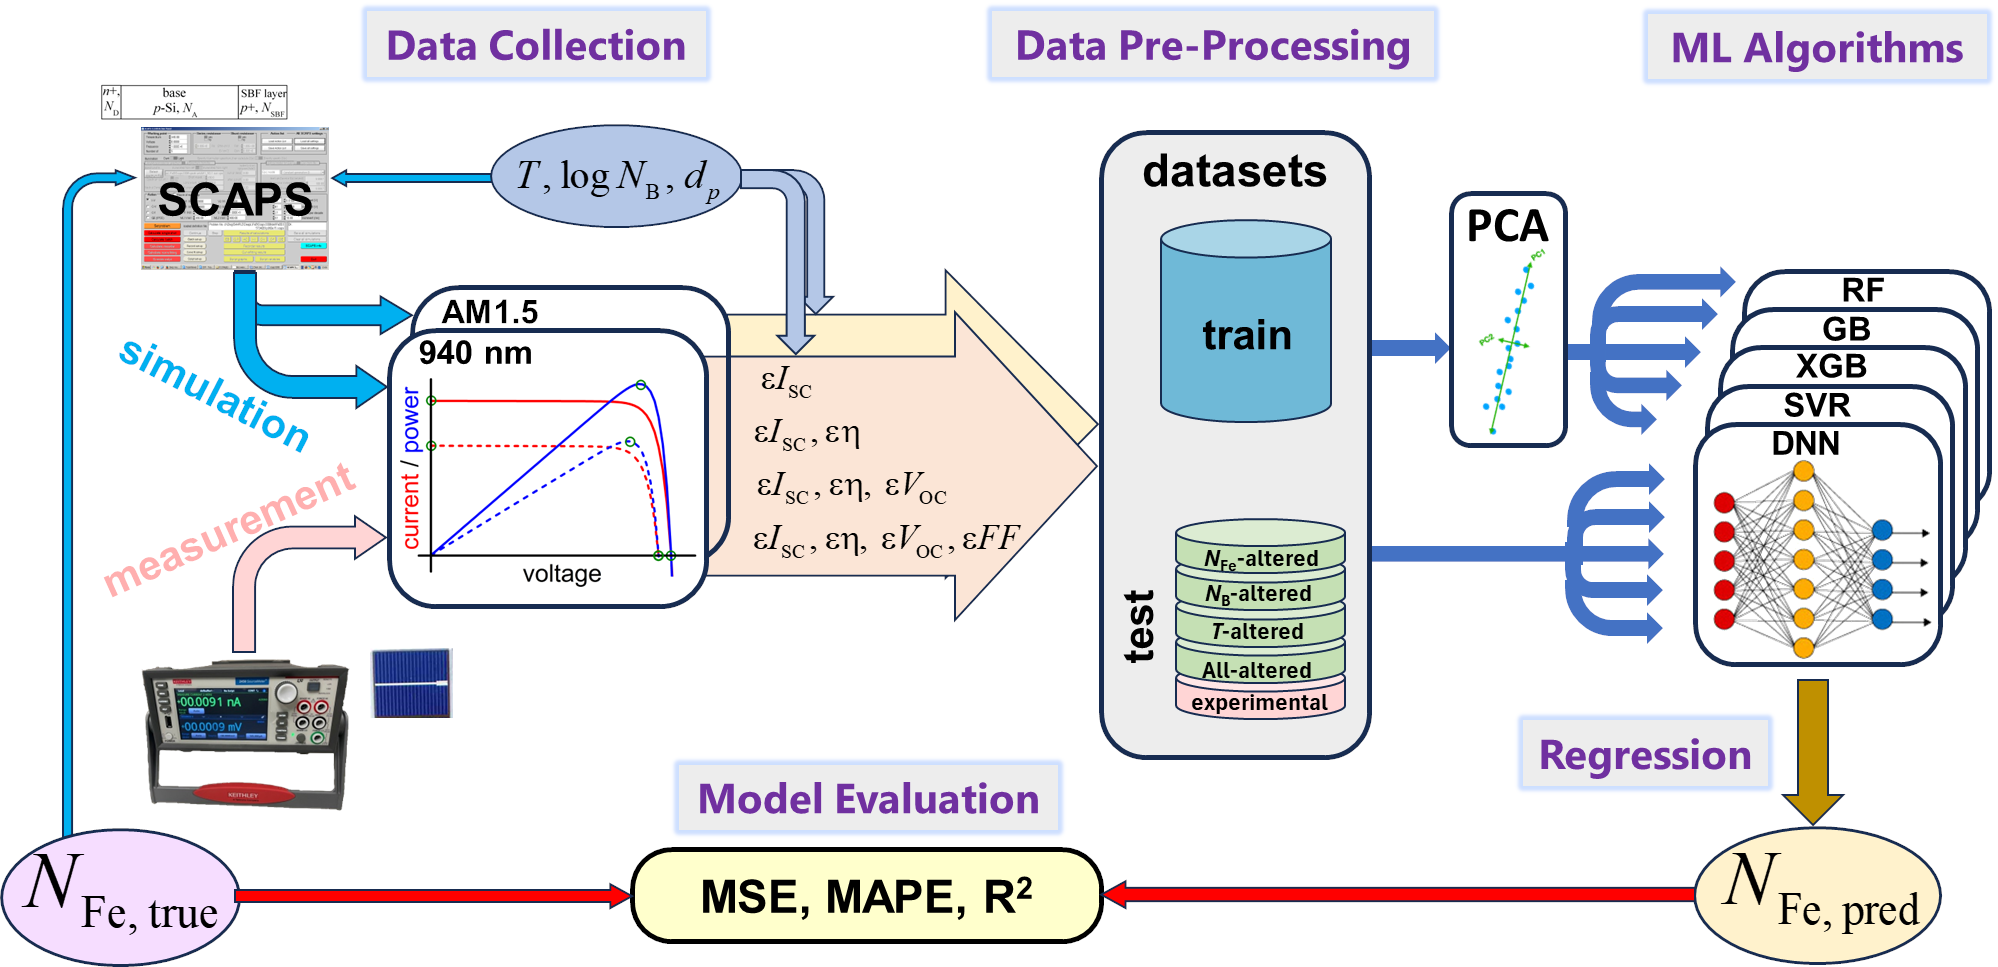
\includegraphics[width=0.9\linewidth]{Fig1.png}
	  \caption{The workflow of the ML pipeline.}\label{fig1}
\end{figure}


\subsection{Data Collection}\label{SecDataCol}

Our research aimed to develop ML models for estimating iron concentration in silicon solar cells.
Selecting relevant descriptors is a critical first step in building robust and effective predictive models.
It is well established that the presence of iron induces the formation of recombination centers, which, in turn, affect the photoelectric conversion process and key PV parameters,
including short-circuit current ($I_\mathrm{SC}$), open-circuit voltage ($V_\mathrm{OC}$), efficiency ($\eta$), and fill factor
(\textcolor[rgb]{1.00,0.07,0.00}{\hl{$F\!F$}}).
Both theoretical and experimental studies \cite{FeB:Schmidt,IronSC,Olikh2025MSEB} have demonstrated that the restructuring of iron-related defects (the dissociation of FeB pairs)
leads to
\textcolor[rgb]{1.00,0.07,0.00}{
\hl{
reversible
}}
variations in PVPs that depend on iron concentration ($N_\mathrm{Fe}$).
As a result, this investigation focused on using iron presence as a descriptor of the relative changes in PVPs caused by the
Fe$_i$B$_\mathrm{Si}$ $\rightleftarrows$ Fe$_i$ + B$_\mathrm{Si}$ reconstruction.
Specifically, the relative changes in short-circuit current, $\varepsilon I_\mathrm{SC}$, were calculated as
\begin{equation}
\label{eq1}
    \varepsilon I_\mathrm{SC} = \frac{I_\mathrm{SC}^\mathrm{FeB} - I_\mathrm{SC}^\mathrm{Fe}}{I_\mathrm{SC}^\mathrm{FeB}} \times 100 \%\,,
\end{equation}
where $I_\mathrm{SC}^\mathrm{FeB}$ and $I_\mathrm{SC}^\mathrm{Fe}$ represent the short--circuit current values before and after pair dissociation, respectively.
The relative changes in the other parameters ($\varepsilon V_\mathrm{OC}$, $\varepsilon \eta$ and $\varepsilon F\!F$) were determined similarly.
Using relative rather than absolute changes helped, to some extent,
isolate iron-related defect contributions from those of other recombination centers
and mitigate potential fluctuations in external conditions, such as illumination intensity.

At the same time, changes in PVPs are shown \cite{FeB:Schmidt,Olikh2025MSEB} to be influenced not only by iron concentration
but also by specific characteristics of the solar cell structure, such as doping level and base thickness,
as well as external factors, including temperature and illumination spectrum.
Therefore, these effects must be considered when selecting an appropriate set of descriptors.
In our study, we incorporated features such as boron concentration in the base ($N_\mathrm{B}$), base thickness ($d_p$), and temperature ($T$)
and developed separate models for different illumination conditions.

For this research, datasets were obtained from both simulations and experiments.
Specifically, $I$-$V$ curve simulations were performed for a silicon $n^+$-$p$-$p^+$ structure using SCAPS~3.3.11.
The SCAPS-1D software \cite{SCAPS1} is a widely used tool
\cite{MasumMia2025, Joshi2024, Ravidas2024, Liu2024, You2023, SCAPSDefect3}
that enables modeling of barrier structure $I$-$V$ characteristics while accounting for defect states.
PVPs were extracted from pairs of $I$-$V$ curves simulated for a solar cell with a known structure
and a specified iron concentration under defined external conditions, both before and after FeB pair dissociation.
This approach allowed us to determine the values of $\varepsilon I_\mathrm{SC}$, $\varepsilon V_\mathrm{OC}$, $\varepsilon \eta$, and
\textcolor[rgb]{1.00,0.07,0.00}{\hl{$\varepsilon F\!F$}}.
A detailed description of the modeling approach, including the used temperature dependencies of silicon and defect parameters,
is provided elsewhere \cite{Olikh2019SM, Olikh2025MSEB}.


To generate the training dataset, we performed simulations over a temperature range of $(290-340)$~K
for solar cells with a base thickness of $(180-380)$~$\mu$m,
a boron concentration of $(10^{15} - 10^{17})$~cm$^{-3}$, and an iron concentration of $(10^{10}-10^{14})$~cm$^{-3}$.
The simulations covered all parameter combinations within a four-dimensional grid, consisting of 11 values along the $T$ axis,
5 along the $d_p$ axis,
9 along the $N_\mathrm{B}$ axis, and 25 along the $N_\mathrm{Fe}$ axis.
The values were evenly distributed within the specified ranges, with $N_\mathrm{B}$ and $N_\mathrm{Fe}$ spaced logarithmically.
Each train dataset consisted of 12,375 samples obtained from simulations of 24,750 $I$-$V$ characteristics.
\textcolor[rgb]{1.00,0.07,0.00}{
\hl{
We emphasize that the parameter values used in our study closely reflect those of real solar cells
and their operating (testing) conditions.
For instance, the selected temperature range corresponds both to the typical operating conditions of most silicon solar cells
and to the (15--75)~$^\circ$C range recommended by the IEC~61215-2:2021 standard for determining the temperature coefficients of PVPs.
}}

We also generated four test datasets through simulation,
each representing different scenarios that may arise in the practical application of ML models.
In one test dataset, the iron concentration values used in the simulation were absent from the training set,
while the other parameters ($T$, $d_p$, $N_\mathrm{B}$) matched the grid node values from the training simulations.
This dataset was designated as ``\textit{$N_\mathrm{Fe}$--altered}'' and contained 1,034 samples.
Similarly, we created the ``\textit{$N_\mathrm{B}$--altered}'' (1,100 samples) and ``\textit{$T$--altered}'' (1,200 samples)
test datasets using boron concentration and temperature values that were not present in the training dataset.
In the ``\textit{All-altered}'' dataset (1,190 samples), all four simulation parameters differed from those used in the training dataset.


The specified simulations for both the training and test datasets were performed under two lighting scenarios:
AM1.5, which corresponds to standard characterization conditions for PV devices,
and monochromatic light with a wavelength of 940~nm and an intensity of 5~W/m$^{2}$,
reflecting the remarkable sensitivity of PVPs to iron \cite{Olikh2025MSEB}.
\textcolor[rgb]{1.00,0.07,0.00}{
\hl{
The obtained parameter limits are as follows:
$\varepsilon I_\mathrm{SC}$ ranges from $-40.88$\% to 6.11\% under AM1.5 illumination and
from $-170.58$\% to 24.66\% under monochromatic light;
$\varepsilon \eta$ ranges from $-50.37$\% to 9.90\% (AM1.5)
and from $-210.32$\% to 31.53\% (monochromatic);
$\varepsilon V_\mathrm{OC}$ ranges from $-12.95$\% to 1.92\%  (AM1.5) and
from $-16.33$\% to 8.15\% (monochromatic);
and $\varepsilon F\!F$ ranges from $-1.42$\% to 11.88\% (AM1.5) and
from $-4.39$\% to 2.98\% (monochromatic).
}}
A total of 67,596 $I$-$V$ curves were simulated.

For experimental validation of the proposed models, we used data obtained from measurements of real solar cells.
We used a set of $n^+$-$p$-$p^+$-Si samples in the experiment.
The structure was fabricated from a 380~$\mu$m thick $p$-type boron-doped Czochralski silicon (100) wafer
with a doping level of $N_\mathrm{B}=1.36\times10^{15}$~cm$^{-3}$.
Iron concentration, determined using the methodology described in \cite{Olikh2022:JMatSci, Olikh2021JAP},
ranged from $2\times10^{11}$ to $4\times10^{13}$~cm$^{-3}$ across different samples.
To create the experimental test dataset,
we measured the $I$-$V$ characteristics under monochromatic illumination from a light-emitting diode (SN–HPIR940nm–1W)
with a wavelength of 940~nm and an intensity of approximately 5~W/m$^{2}$, within a temperature range of $(305-340)$~K.
The decay of FeB pairs was induced using intensive halogen lamp illumination (7000~W/m$^{2}$).
\textcolor[rgb]{1.00,0.07,0.00}{
\hl{
In general, the dissociation rate of FeB pairs depends on the illumination intensity, $N_\mathrm{Fe}$ }
\cite{FeBLight2,FeBAssJAP2014,FeMethod2012},
temperature \cite{lauer2016},
the spectral composition of illumination \cite{OlikhPSSA},
and the presence of recombination channels other than those associated with iron-related defects \cite{FeBLight2,FeBAssJAP2014}.
The selected illumination duration required to achieve near-complete dissociation depended on the iron concentration
and reached up to 400~s for the solar cells with the highest $N_\mathrm{Fe}$ values.
The illumination intervals were determined based on the results of a previous study \cite{OlikhPSSA},
\hl{which showed that under similar conditions, complete dissociation at $N_\mathrm{Fe}=9\times10^{12}$~cm$^{-3}$ occurred within 20~s.
}}
The number of samples in experimental dataset varied from 34 to 12, depending on the feature dimensionality.


\subsection{Data Pre-Processing}

Feature selection is a crucial pre-processing step in developing a forecasting model.
Selecting the appropriate number of features requires balancing two competing factors.
On one hand, fewer features simplify data collection and reduce computational costs.
On the other hand, incorporating more features may enhance prediction accuracy by providing additional information.
In this study, various feature combinations were explored.
As shown in \cite{Olikh2025MSEB}, $\varepsilon I_\mathrm{SC}$ is a key metric for quantifying iron impurities
due to its monotonic dependence on iron concentration and relatively large absolute values during the
Fe$_i$B$_\mathrm{Si}$ $\rightleftarrows$ Fe$_i$ + B$_\mathrm{Si}$
transformation.
The following most suitable parameters for estimating $N_\mathrm{Fe}$ are
$\varepsilon \eta$, $\varepsilon V_\mathrm{OC}$, and $\varepsilon F\!F$ \cite{Olikh2025MSEB}.

Moreover, $N_\mathrm{B}$ (one of the selected descriptors) and
$N_\mathrm{Fe}$ (target output) span several orders of magnitude.
To achieve high prediction accuracy, we transformed the doping level and iron concentration into
$\log N_\mathrm{B}$ and $\log N_\mathrm{Fe}$.
This approach is standard for quantities that vary over a wide range \cite{Srivastava2023, Minagawa2024}.

Thus, we used the following sets to predict $y = \log N_\mathrm{Fe}$:
($T$, $d_p$, $N_\mathrm{B}$, $\varepsilon I_\mathrm{SC}$);
($T$, $d_p$, $N_\mathrm{B}$, $\varepsilon I_\mathrm{SC}$, $\varepsilon \eta$);
($T$, $d_p$, $N_\mathrm{B}$, $\varepsilon I_\mathrm{SC}$, $\varepsilon \eta$, $\varepsilon V_\mathrm{OC}$);
($T$, $d_p$, $N_\mathrm{B}$, $\varepsilon I_\mathrm{SC}$, $\varepsilon \eta$, $\varepsilon V_\mathrm{OC}$, $\varepsilon F\!F$).
For simplicity, we will refer to the number of features as ``dimension'' from here on.
That is, features with dimensions 4, 5, 6, and 7 were used in various models.
\textcolor[rgb]{1.00,0.07,0.00}{
\hl{
When selecting sets of descriptors, we were guided by the degree of correlation between variations in individual PVPs and iron concentration
(see Fig.~S1 in the Supplementary Material).
Specifically, the 4-dimensional feature set included the measurement conditions ($T$),
solar cell characteristics ($d_p$ and $N_\mathrm{B}$), and the PVP most strongly correlated with $\log N_\mathrm{Fe}$, $\varepsilon I_\mathrm{SC}$.
In extending the set to five dimensions, we added the parameter most strongly correlated with $N_\mathrm{Fe}$
among the remaining unused ones --- namely,  $\varepsilon \eta$  --- to the existing features.
Subsequent steps followed a similar procedure.
}}

Data normalization transforms a dataset's values to a standard scale, which can improve model accuracy.
To standardize our features, we normalized them to have a mean of zero and a standard deviation of one.

Increasing the number of features does not always enhance informativeness if the descriptors are not independent.
This study used the Pearson correlation coefficient to assess the relationships between input features.
We found that changes in PV parameters are not entirely independent, particularly under monochromatic illumination
(see Fig.~S1).
This is not surprising, since each of the PV parameters is linked to the diffusion and recombination of photo-induced charge carriers.
Besides,
$\varepsilon I_\mathrm{SC}$, $\varepsilon V_\mathrm{OC}$, $\varepsilon \eta$, and $\varepsilon F\!F$
exhibit a strong correlation with boron concentration.
$N_\mathrm{B}$ determines the position of the Fermi level, which, in turn, significantly influences
the intensity of recombination processes within the Shockley–Read–Hall approximation.
This provides the physical basis for the observed correlation.

To ensure that ML algorithms are trained on independent input features while reducing data redundancy and memory usage,
we applied Principal Component Analysis (PCA).
PCA constructs new, uncorrelated features (principal components, PCs) and allows us to evaluate each PC's contribution to the total variance.
Fig.\ref{fig2} shows that increasing the feature dimension does not always enhance overall information variance.
To assess the impact of redundant data, we trained ML models using features selected as follows:
we computed PCs for the original dataset and then reduced the total dimension
by discarding PCs whose contribution to the total variance was below 1.5\%.
The final dimensions of the different feature sets are provided in Table~\ref{tbl1}.
\textcolor[rgb]{1.00,0.07,0.00}{
\hl{
In general, PCA is a widely used and effective tool in machine learning,
particularly for addressing problems in photovoltaics.
For example, it has been successfully applied to fault detection and classification based on $I$-$V$ curves} \cite{Fadhel2019, Gao2020},
performance prediction of organic \cite{David2021} and perovskite \cite{Liu2022} solar cells,
as well as measurement of the internal quantum efficiency in GaAs solar cells \cite{AbdullahVetter2025}.
}

\begin{figure}
	\centering
     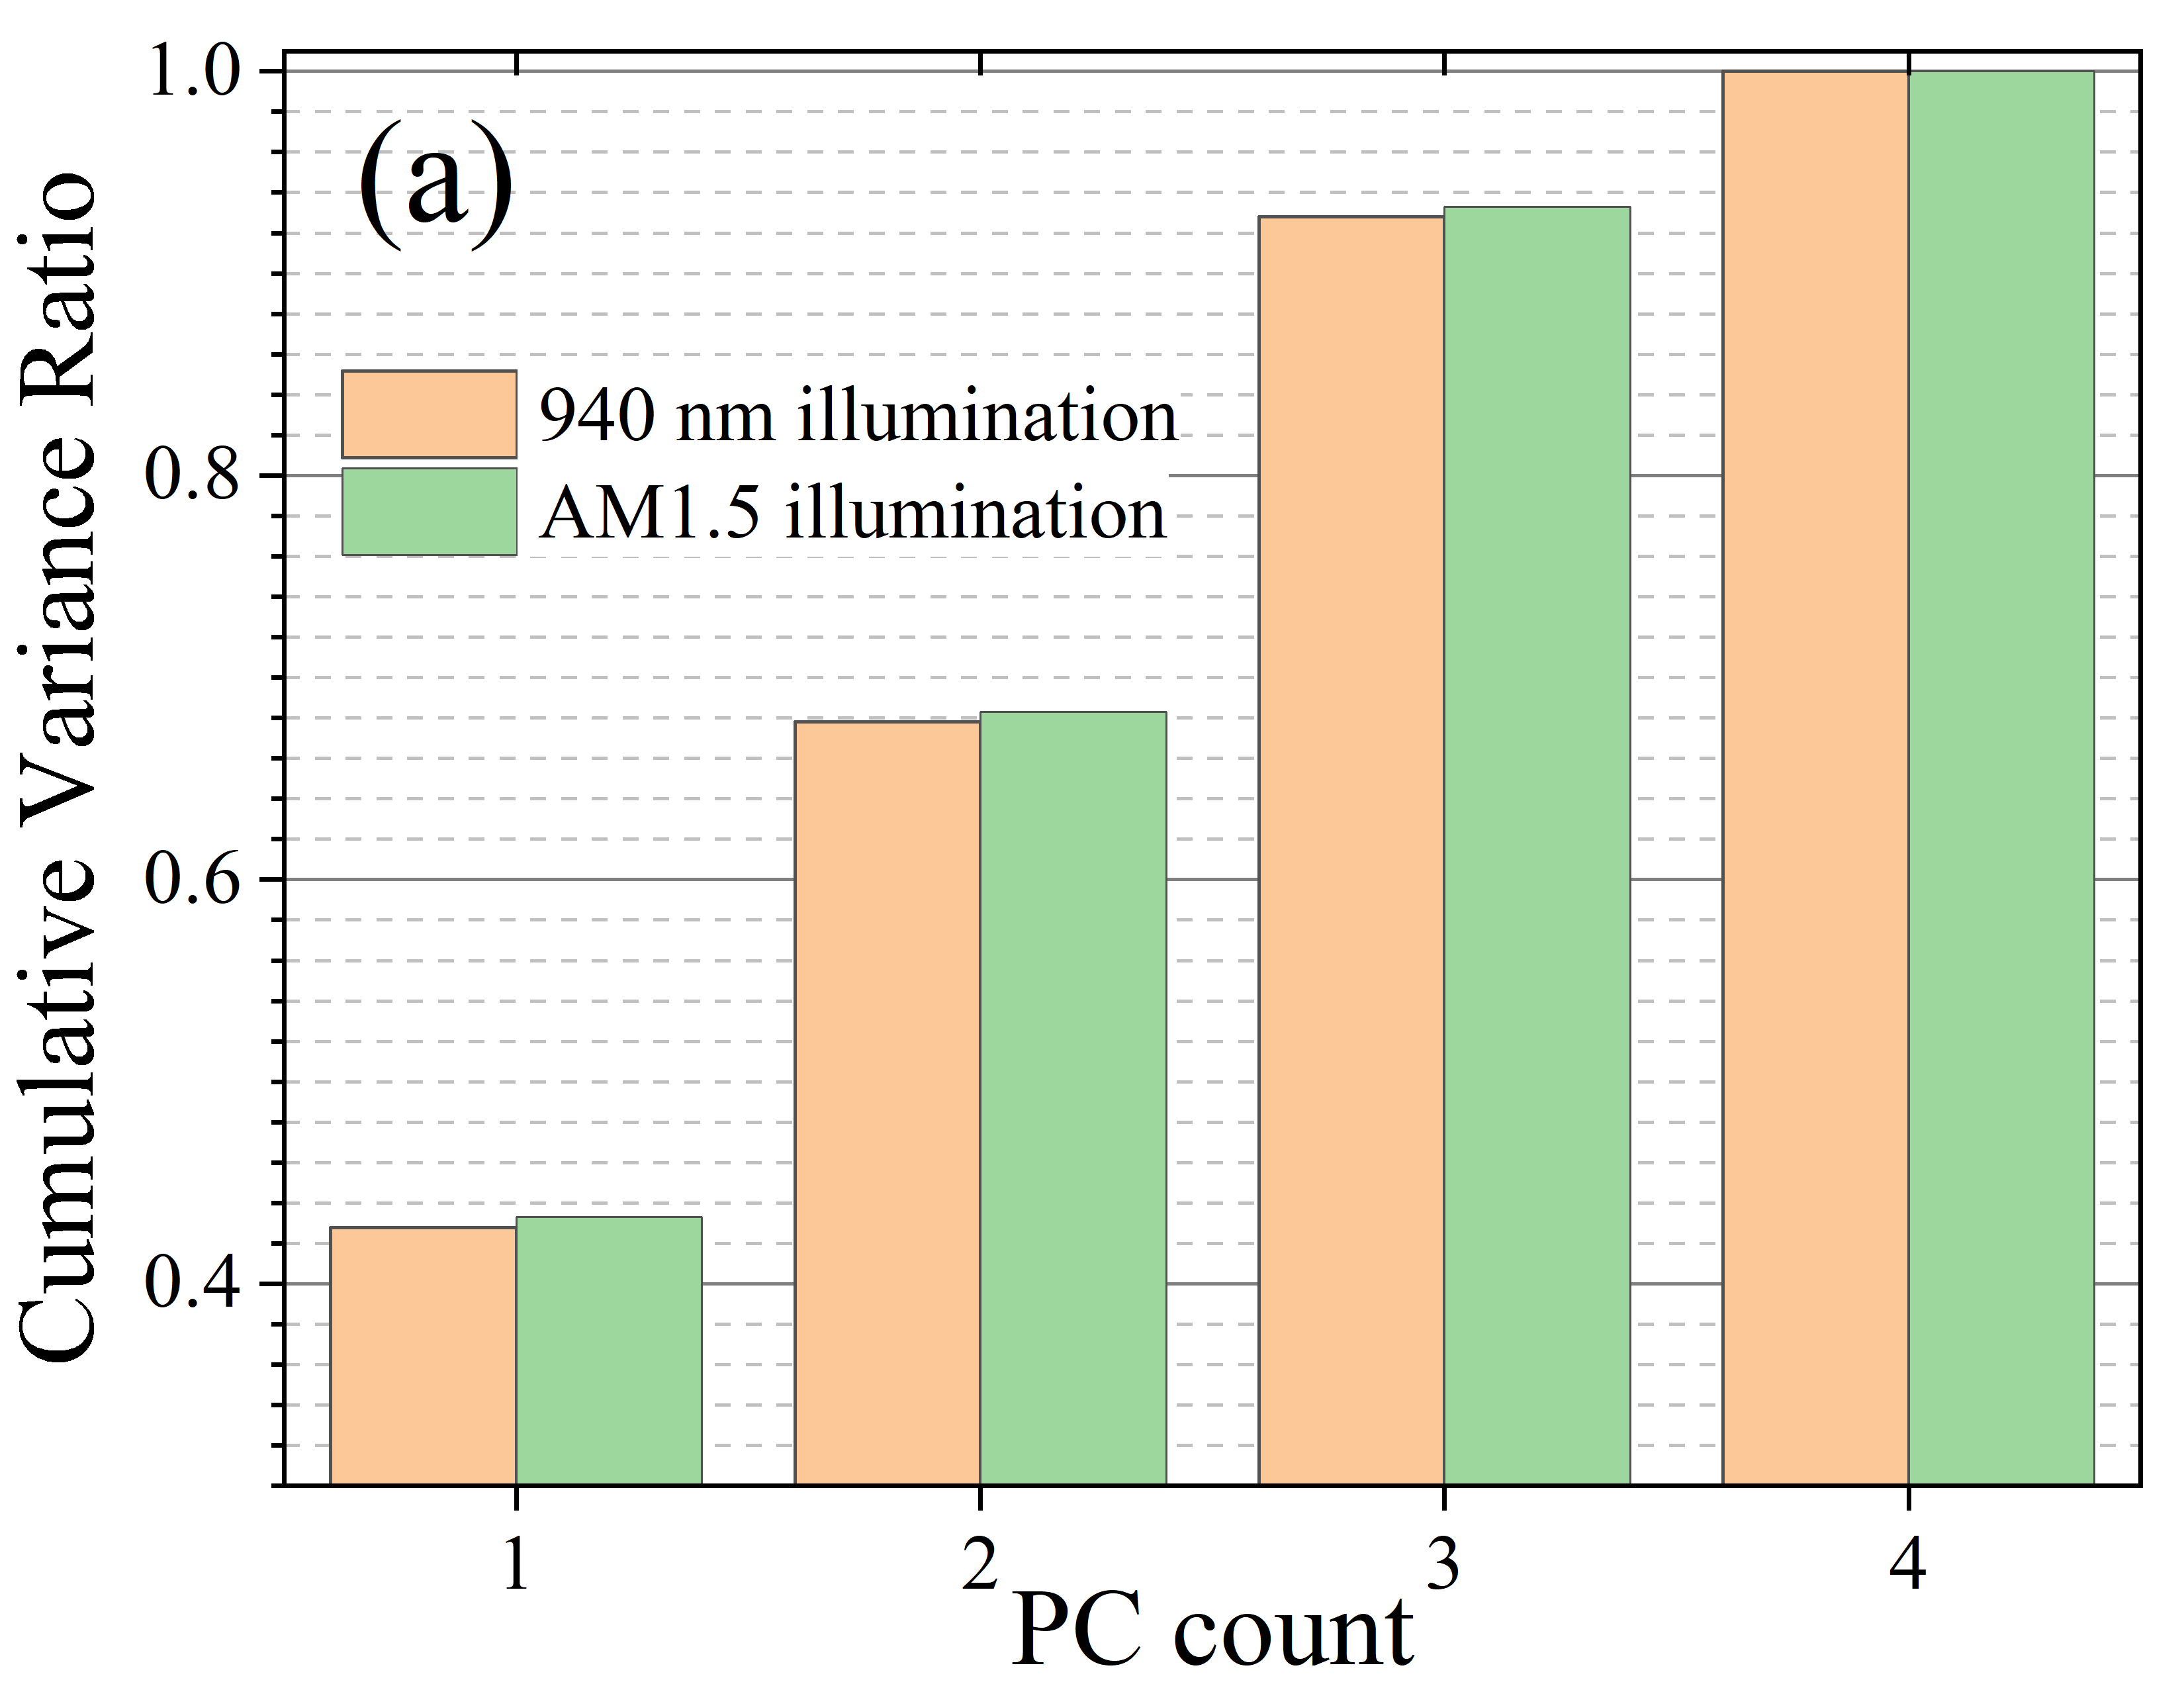
\includegraphics[width=0.24\linewidth]{Fig2a.png}
     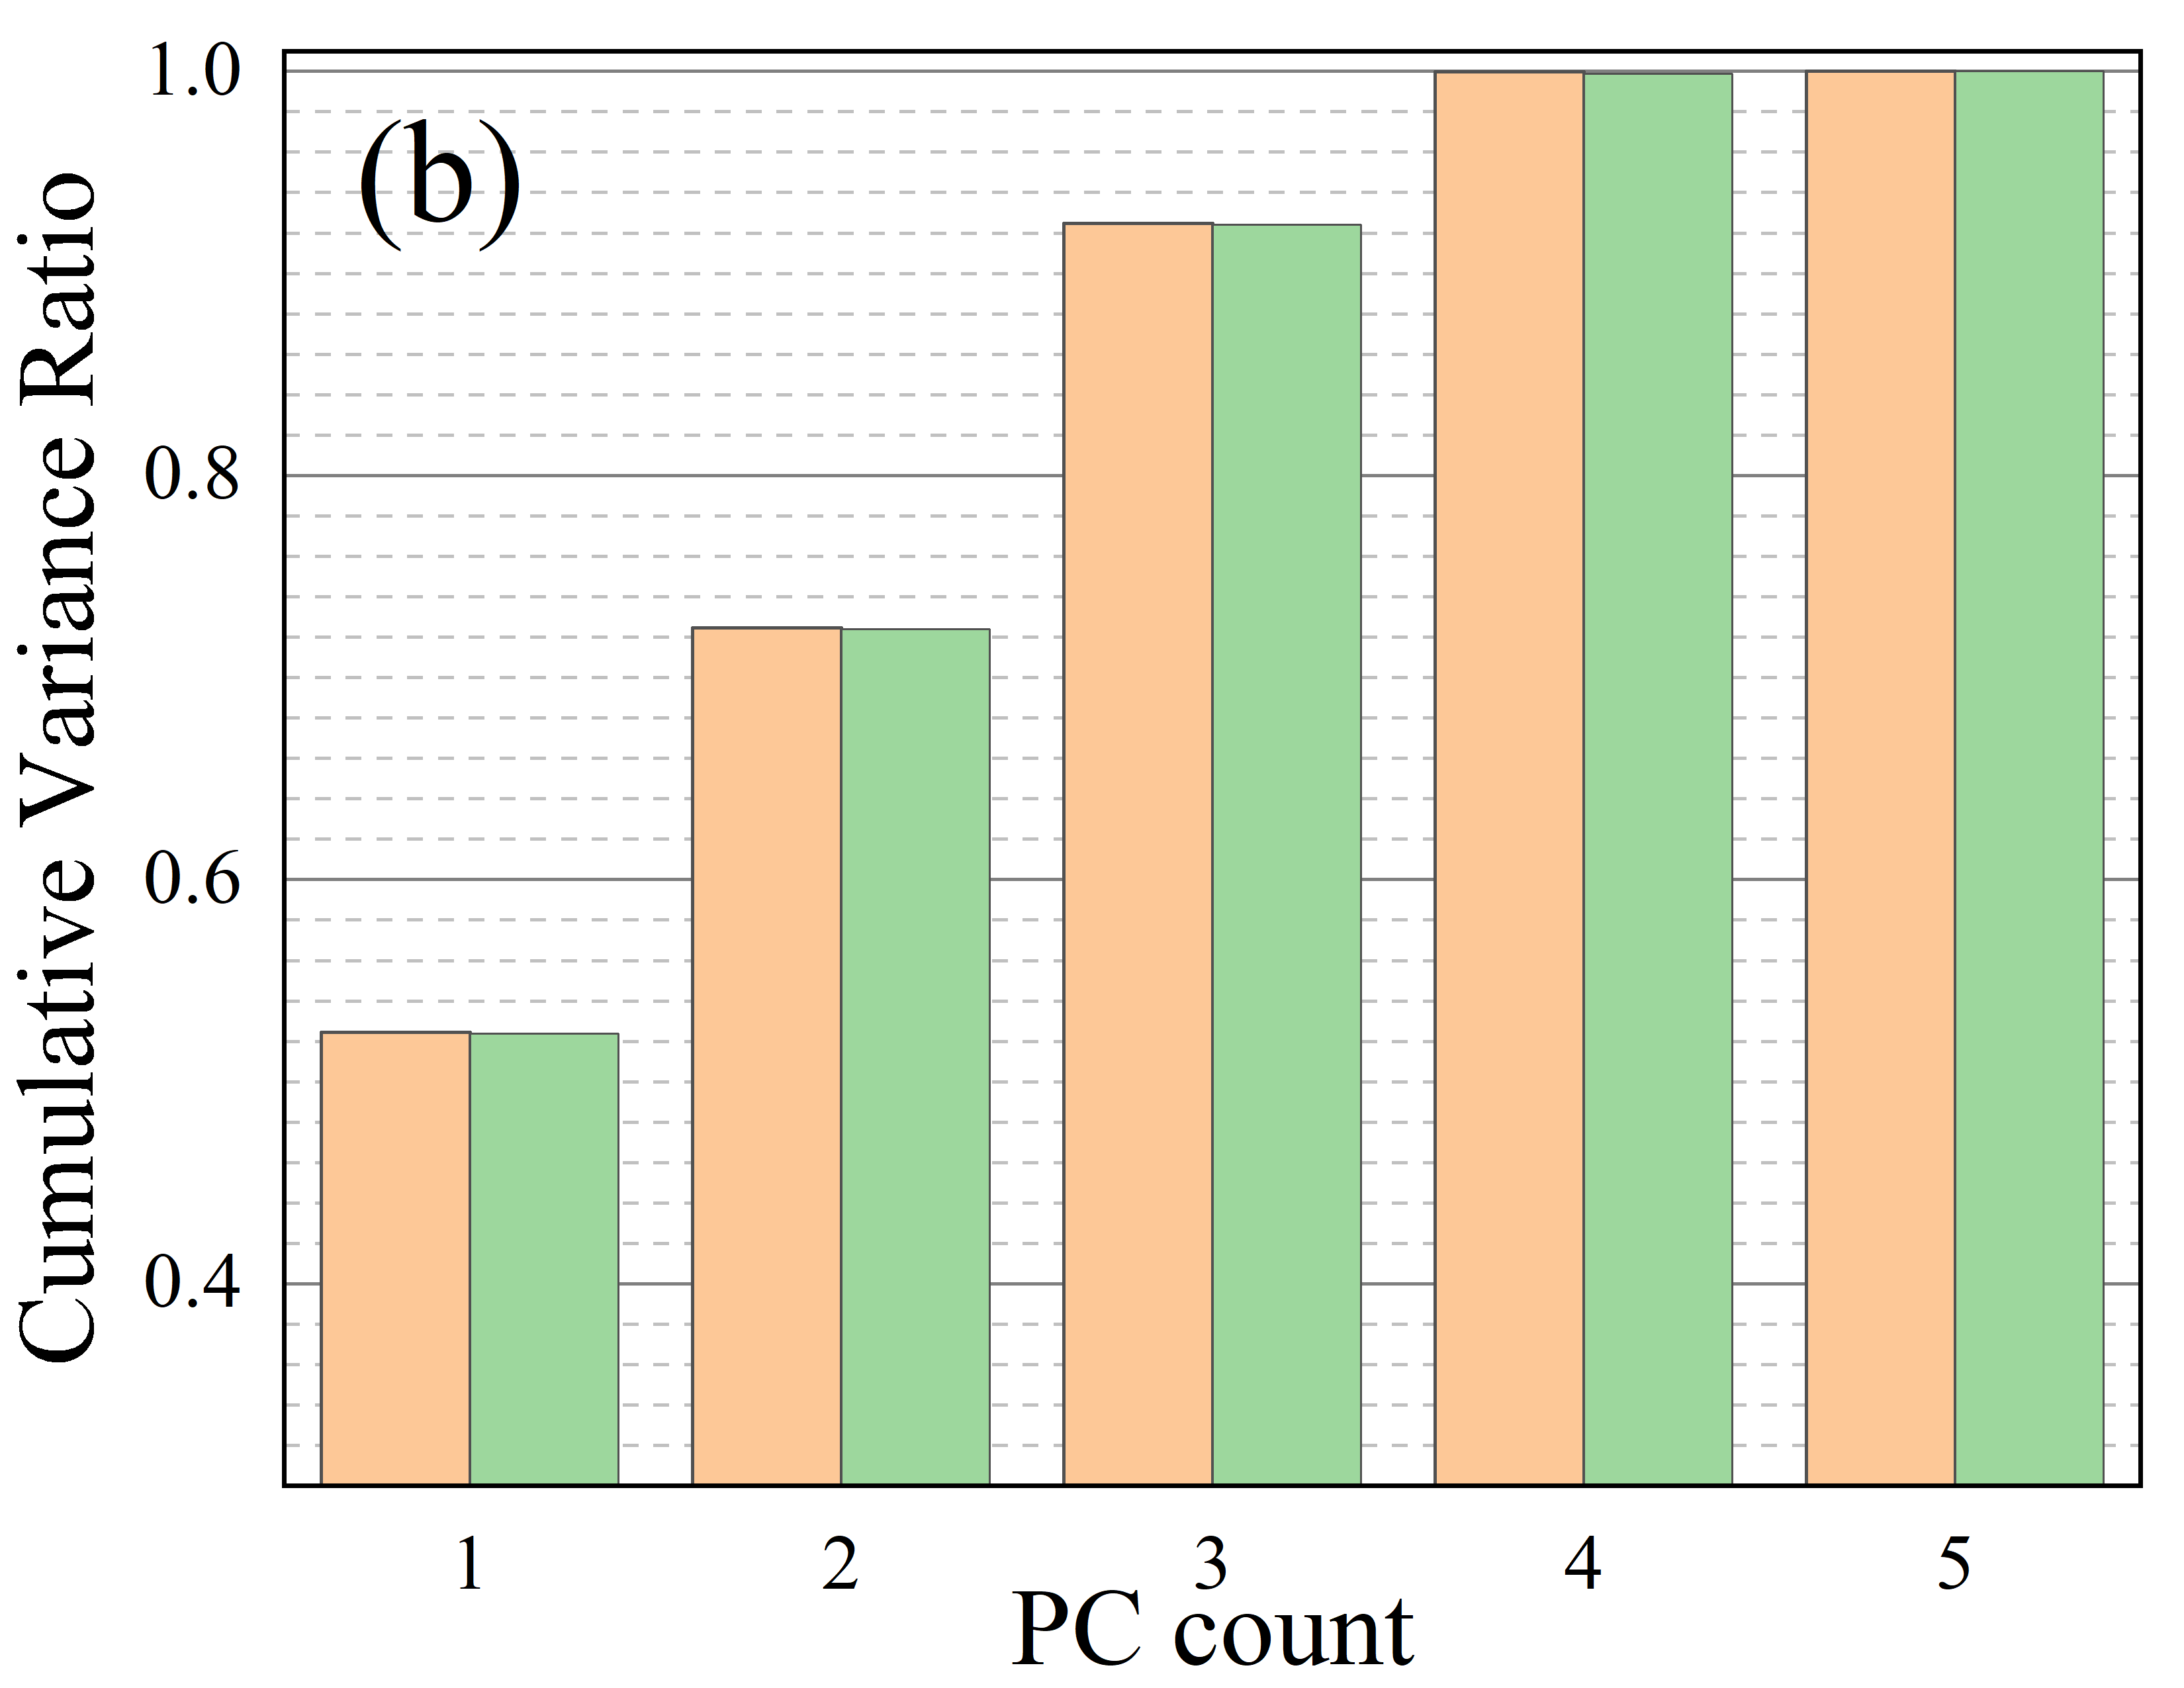
\includegraphics[width=0.24\linewidth]{Fig2b.png}
     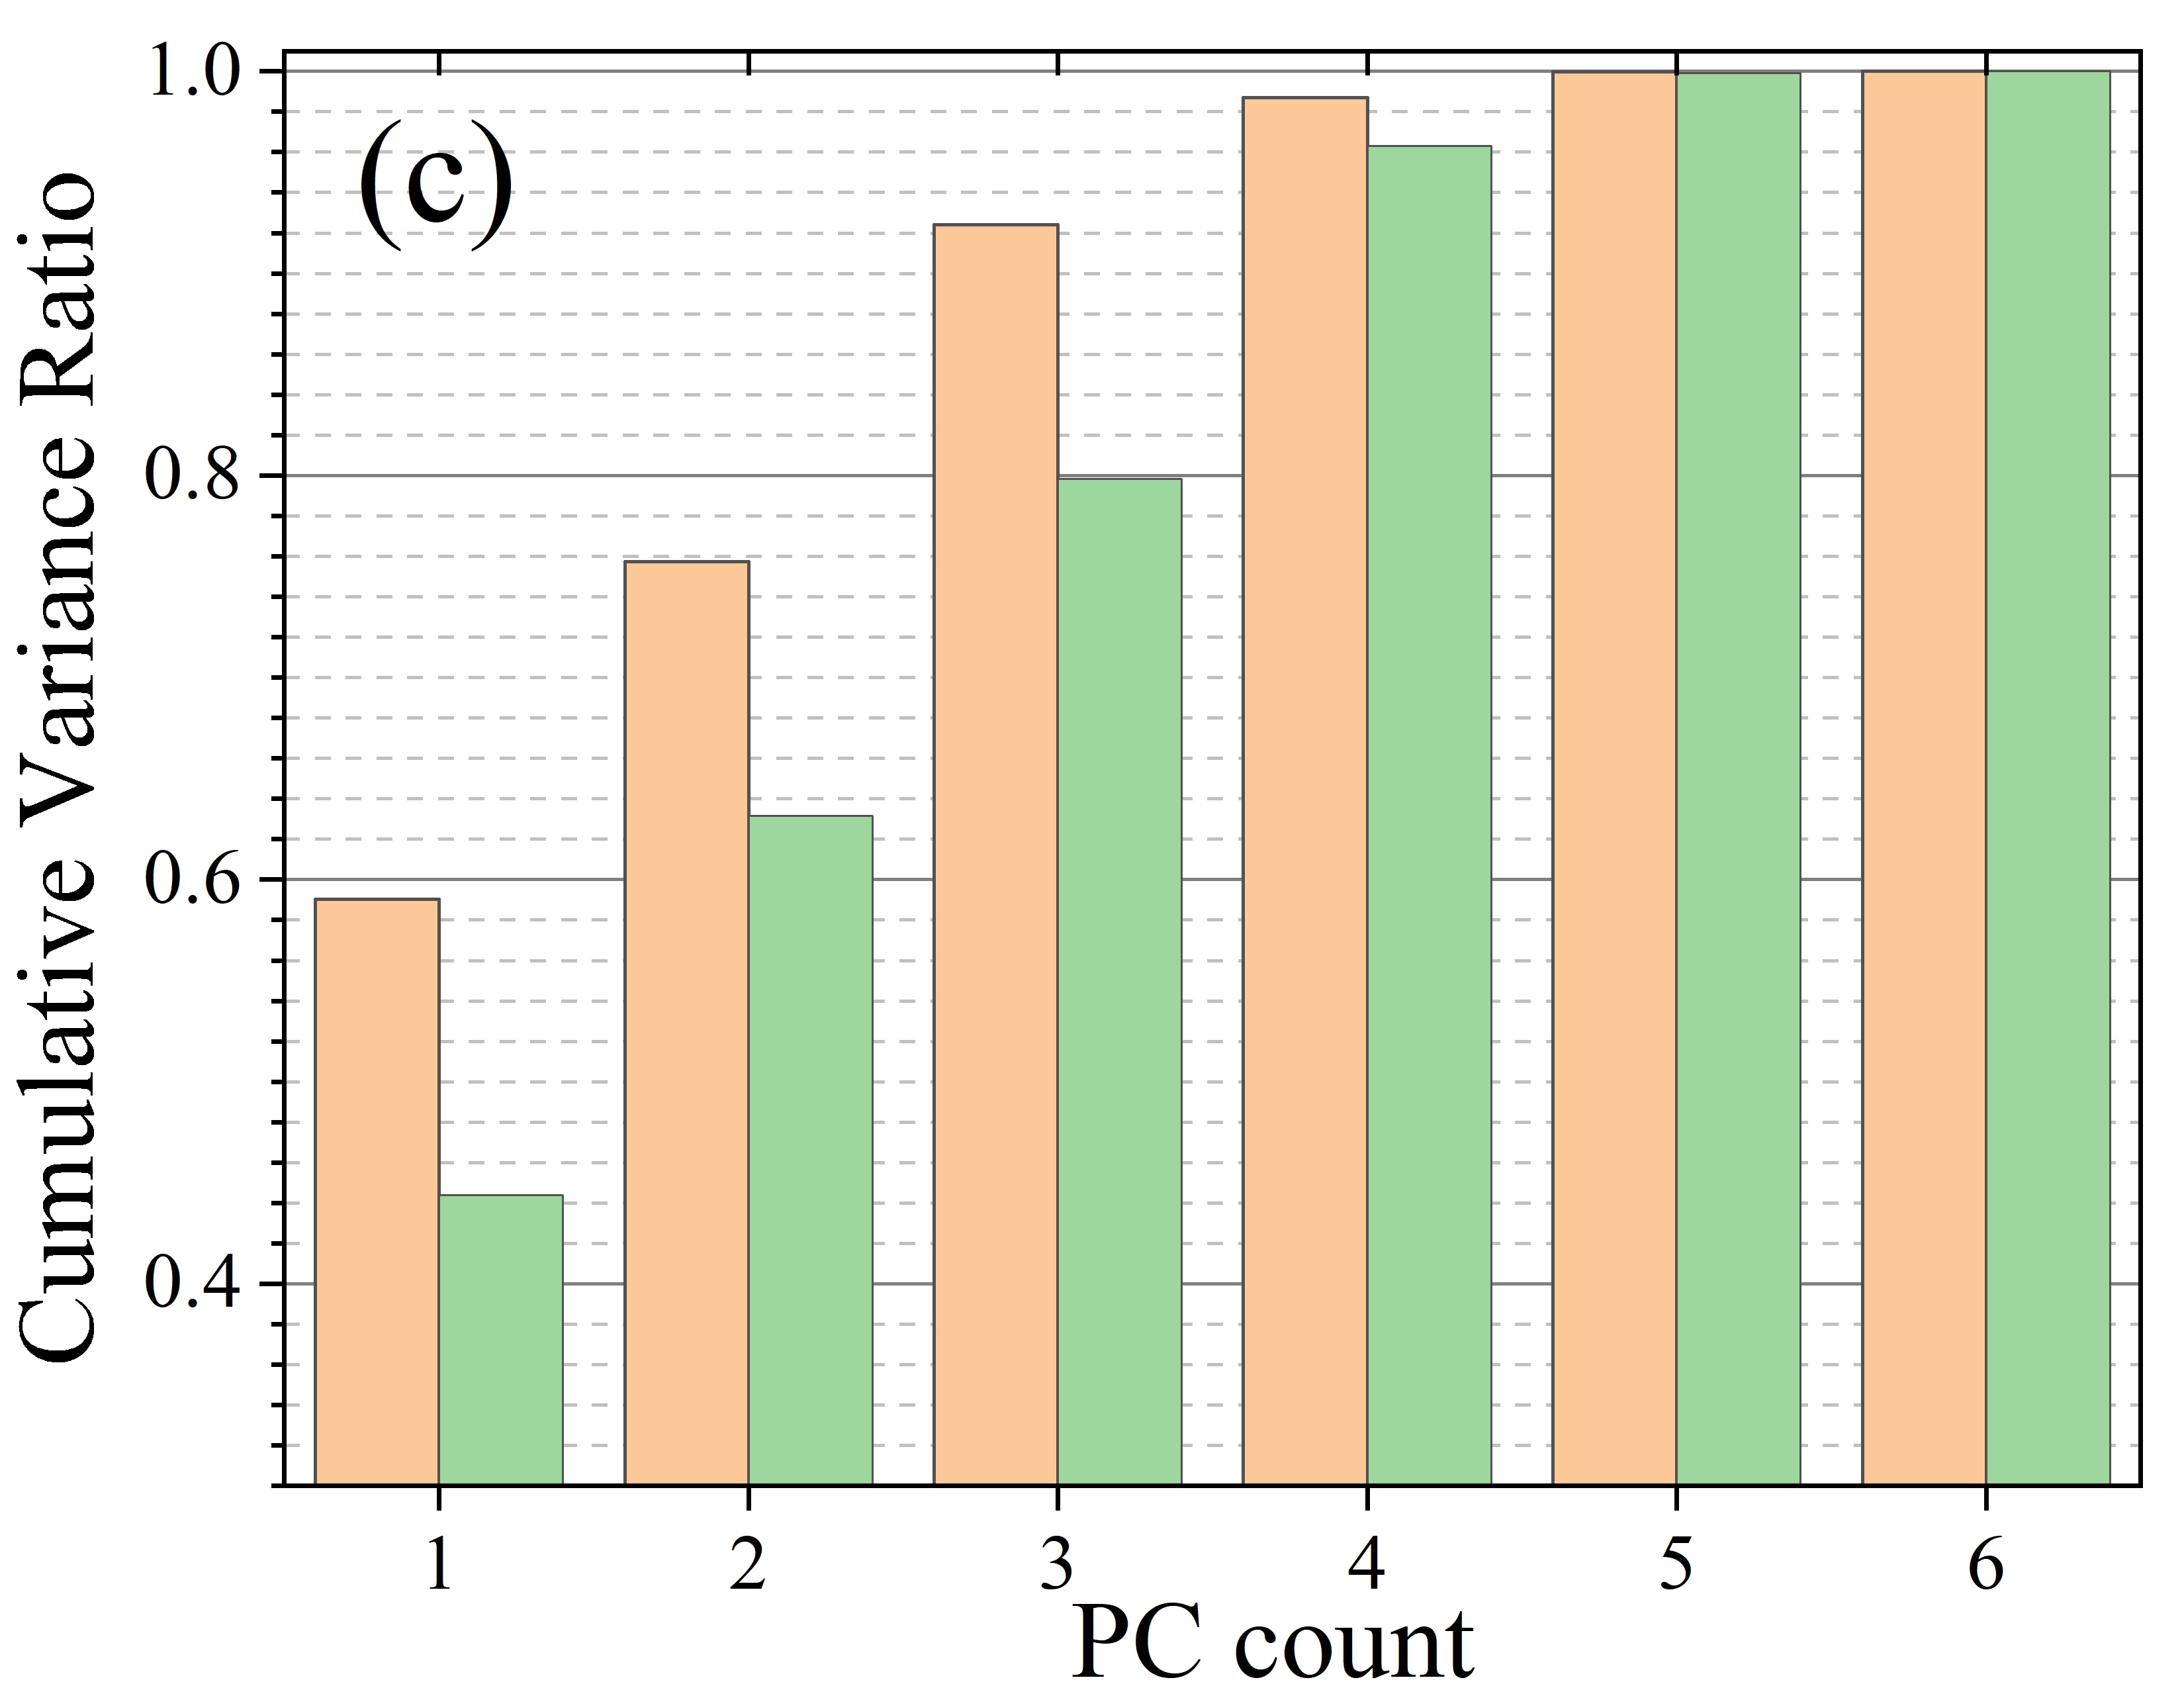
\includegraphics[width=0.24\linewidth]{Fig2c.png}
     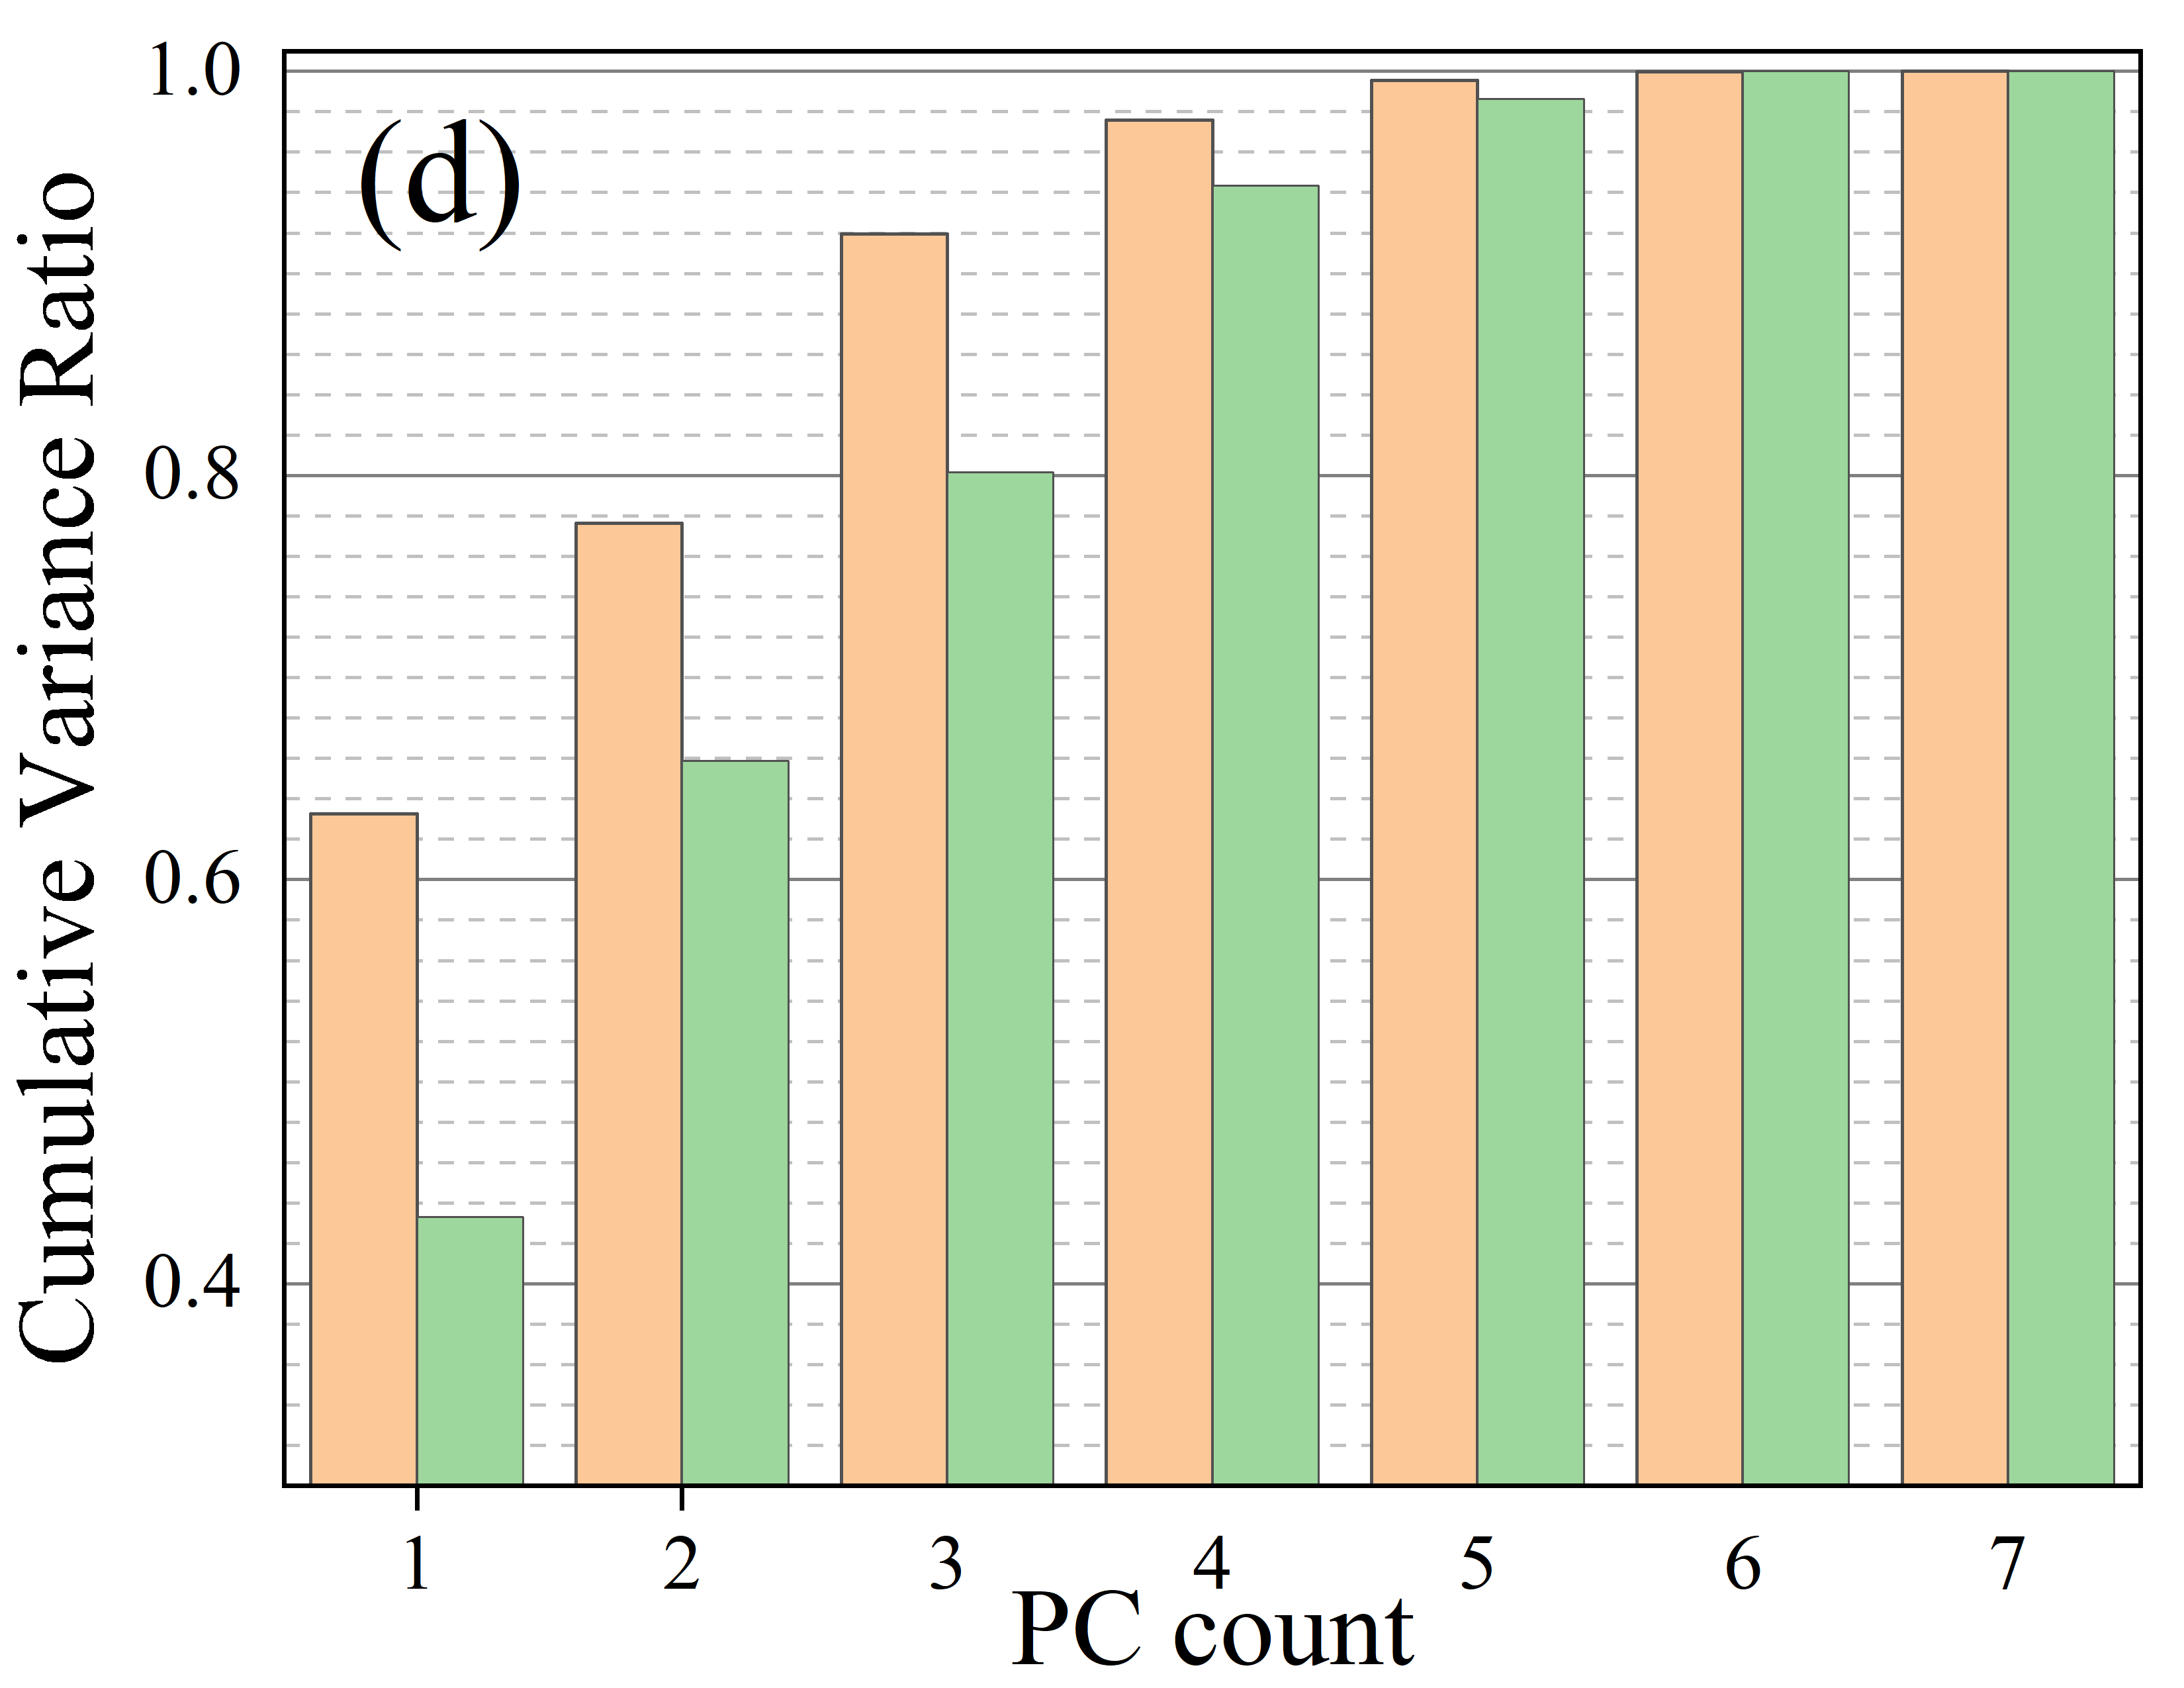
\includegraphics[width=0.24\linewidth]{Fig2d.png}
	  \caption{Cumulative explained variance versus number of PC components.
Feature dimension: 4 (a), 5 (b), 6 (c), 7 (d).
}\label{fig2}
\end{figure}

\begin{table}[<options>]
\caption{Feature dimension after PCA applying}
\label{tbl1}
\begin{tabular*}{\tblwidth}{@{}LCC@{}}
\toprule
\multirow{2}{*}{Initial dimension}
&\multicolumn{2}{C}{Final dimension}\\
&AM1.5 illumination&940~nm illumination\\% Table header row
\midrule
4&4&4\\
5&4&4\\
6&5&4\\
7&6&5\\
\bottomrule
\end{tabular*}
\end{table}

\subsection{Machine Learning Algorithms}

We used five ML algorithms to develop regression models for predicting iron concentration.

\emph{Random Forest} (RF) improves predictive accuracy by training multiple decision trees on different subsets of the dataset.
RF aggregates predictions from all trees using majority voting for classification or averaging for regression,
reducing overfitting and increasing robustness to noise \cite{Breiman2001}.

\emph{Gradient Boosting} (GB) combines multiple weak learners, typically decision trees, to improve predictive performance.
It sequentially adds predictors, with each new model correcting the errors of its predecessor, thereby enhancing overall accuracy.
The final prediction is obtained by aggregating forecasts, usually through a weighted sum \cite{Natekin2013}.

\emph{eXtreme Gradient Boosting} (XGB) is an advanced ensemble method for gradient boosting machines \cite{Akinpelu2024}.
Unlike standard GB, XGB utilizes the Newton–Raphson method with second-order derivatives of the loss function,
improving accuracy, computational speed, and efficiency for large datasets.

\emph{Support Vector Regression }(SVR) finds a hyperplane that maximizes the margin while minimizing errors within a specified tolerance.
It maps input data into a high-dimensional feature space using kernel functions, effectively capturing nonlinear relationships \cite{Cao2020}.

\emph{Deep Neural Network} (DNN) comprises multiple layers of interconnected neurons that process input data
through successive nonlinear transformations \cite{Liu2023}.

It is worth noting that all the algorithms used have demonstrated effectiveness in previous
defect studies \cite{Buratti2020a, Buratti2022, Olikh2022PPV, Buratti2024}.

Considering different machine learning algorithms, data collected under various lighting conditions,
features with varying dimensions, and the inclusion or exclusion of PCA, we evaluated 80 distinct models.
From this point forward, the models will be referred to as
\begin{equation*}
    \mathrm{A}^\mathrm{illum}_\mathrm{feat},
\end{equation*}
where ``A'' represents the ML algorithm used,
and it can take one of the following values: (RF, GB, XGB, SVR, DNN);
``illum'' indicates the solar cell illumination type: illum $\in$ (AM1.5, 940);
``feat'' represents the feature dimension and the application of PCA,
where $\mathrm{feat} \in (4, 5, 6, 7, 4\text{:PC}, 5\text{:PC}, 6\text{:PC}, 7\text{:PC})$.

The models are implemented using Python toolkits: Keras for DNN, Scikit-learn for RF, GB, and SVR, and XGBoost for XGB.
Hyperparameter tuning is known \cite{Hanif2024} to be essential for optimizing model performance.
We used the Optuna toolkit to optimize model parameters, employing the TPE sampler and Hyperband pruner for efficient hyperparameter selection.
Tables~S1--S5 (Supplementary Material) provide the tuned hyperparameters and their search ranges.
It is worth noting that 5-fold cross-validation was employed during the model tuning process,
with 20\% of the train data used as the validation set to evaluate models trained on the remaining 80\%.
The chosen hyperparameter combinations are presented in Tables~S6--S10.


\subsection{Model evaluation}

To build a regression model, it is crucial to evaluate its performance using various metrics.
These metrics assess how well the model has learned and predicted outcomes.
The evaluation metrics for iron quantification were the mean squared error (MSE),
mean absolute percentage error (MAPE),
and coefficient of determination (R$^2$), as defined in Eqs.~(\ref{eq3})–(\ref{eq5}).
\begin{equation}
\label{eq3}
    \mathrm{MSE} = \frac{1}{N}\displaystyle\sum_{i=1}^{N} (\hat{y_i}-y_i)^2\,,
\end{equation}
where $\hat{y_i}$ represents the predicted value for the $i$--th data point,
$y_i$ is the known value for the $i$--th data point,
and $N$ is the number of samples in the dataset.
MSE is one of the most commonly used metrics for evaluating model accuracy.
However, since the computation of $\hat{y_i}$ involves the normalization and logarithm transformation of $N_\mathrm{Fe}$,
this metric does not fully reflect the accuracy of iron contamination estimation.
Therefore, we used MAPE, which determines the mean relative error:
\begin{equation}
\label{eq4}
    \mathrm{MAPE} = \frac{1}{N}\displaystyle\sum_{i=1}^{N} \frac{|N_{\mathrm{Fe,PRED},i}-N_{\mathrm{Fe,TRUE},i}|}{N_{\mathrm{Fe,TRUE},i}}\times 100 \%\,,
\end{equation}
where $N_{\mathrm{Fe,PRED},i}$ is the predicted value of iron concentration,
$N_{\mathrm{Fe,TRUE},i}$ is the known value (used in simulation or obtained from experimental iron determination).

The $R^2$ score is often interpreted as the percentage of explained variance
and measures how well the predicted and true values align; a value of unity indicates a perfect prediction:
\begin{equation}
\label{eq5}
    \mathrm{R}^2 = 1-\frac{\displaystyle\sum_{i=1}^{N} (N_{\mathrm{Fe,TRUE},i}-N_{\mathrm{Fe,PRED},i})^2}
    {\displaystyle\sum_{i=1}^{N} (N_{\mathrm{Fe,TRUE},i}-\overline{N_\mathrm{Fe,TRUE}})^2},
\end{equation}
where $\overline{N_\mathrm{Fe,TRUE}}$ is the mean of the true values.

In particular, Table~S11 (Supplementary Materials) presents the performance metrics obtained
using 5-fold cross-validation on the train dataset with the selected hyperparameter combinations.


The MSE and MAPE are highly sensitive to even a few low-accuracy predictions.
To better assess the models and account for the impact of individual outliers, we also used the median absolute percentage error (MdAPE),
which indicates the error value below which 50\% of the predictions in the dataset fall.
Furthermore, we evaluated the metric $p$, representing the percentage of samples (feature vectors) in a dataset with an absolute error below a specified threshold.
Specifically, we computed the values of $p01$ and $p10$,
which represent the proportion of predictions in the dataset with an accuracy of 1\%
or better and 10\% or better, respectively.
The decrease in MdAPE and the increase in $p01$ and $p10$ indicate improved model performance
due to a higher proportion of accurate predictions.


%\cite{Pata2024, Holechek2022,Park2022,Qi2020,Rachdi2021,Buratti2020,Zhang2022,Liu2023,Asghar2023,AbdullahVetter2025,DiSabatino2024,Datta2023,Jaiswal2023,Buratti2024,Bhatti2023,AlOtum2024,
%Pratt2021,Li2024a,Lin2021,Tang2020,Bu2022,Turek2023,Huang2022,Chen2019,Hopwood2020,Mellit2021,Ma2025,Choudhary2023,Chia2024,Wang2024a,Buratti2022,Buratti2020a,Le2024,Yamaguchi2018,Bosnjakovic2024,
%Zhang2021,DiSabatino2014,Kunze2023,Battaglia2023,Minagawa2024,Breiman2001,Natekin2013,Akinpelu2024,Cao2020,Hanif2024}

\section{Results and Discussion}

\subsection{Train dataset}

Fig.~\ref{fig3} presents the models’ prediction results on the training set.
The Supplementary Materials (Figs.~S4--S7) provide more detailed results, while Tables~S12 and S13 list the performance metrics.
The RF and GB models yield the most accurate predictions, whereas SVR performs the worst.
Applying PCA generally reduces prediction accuracy on the training set.

\begin{figure}
	\centering
     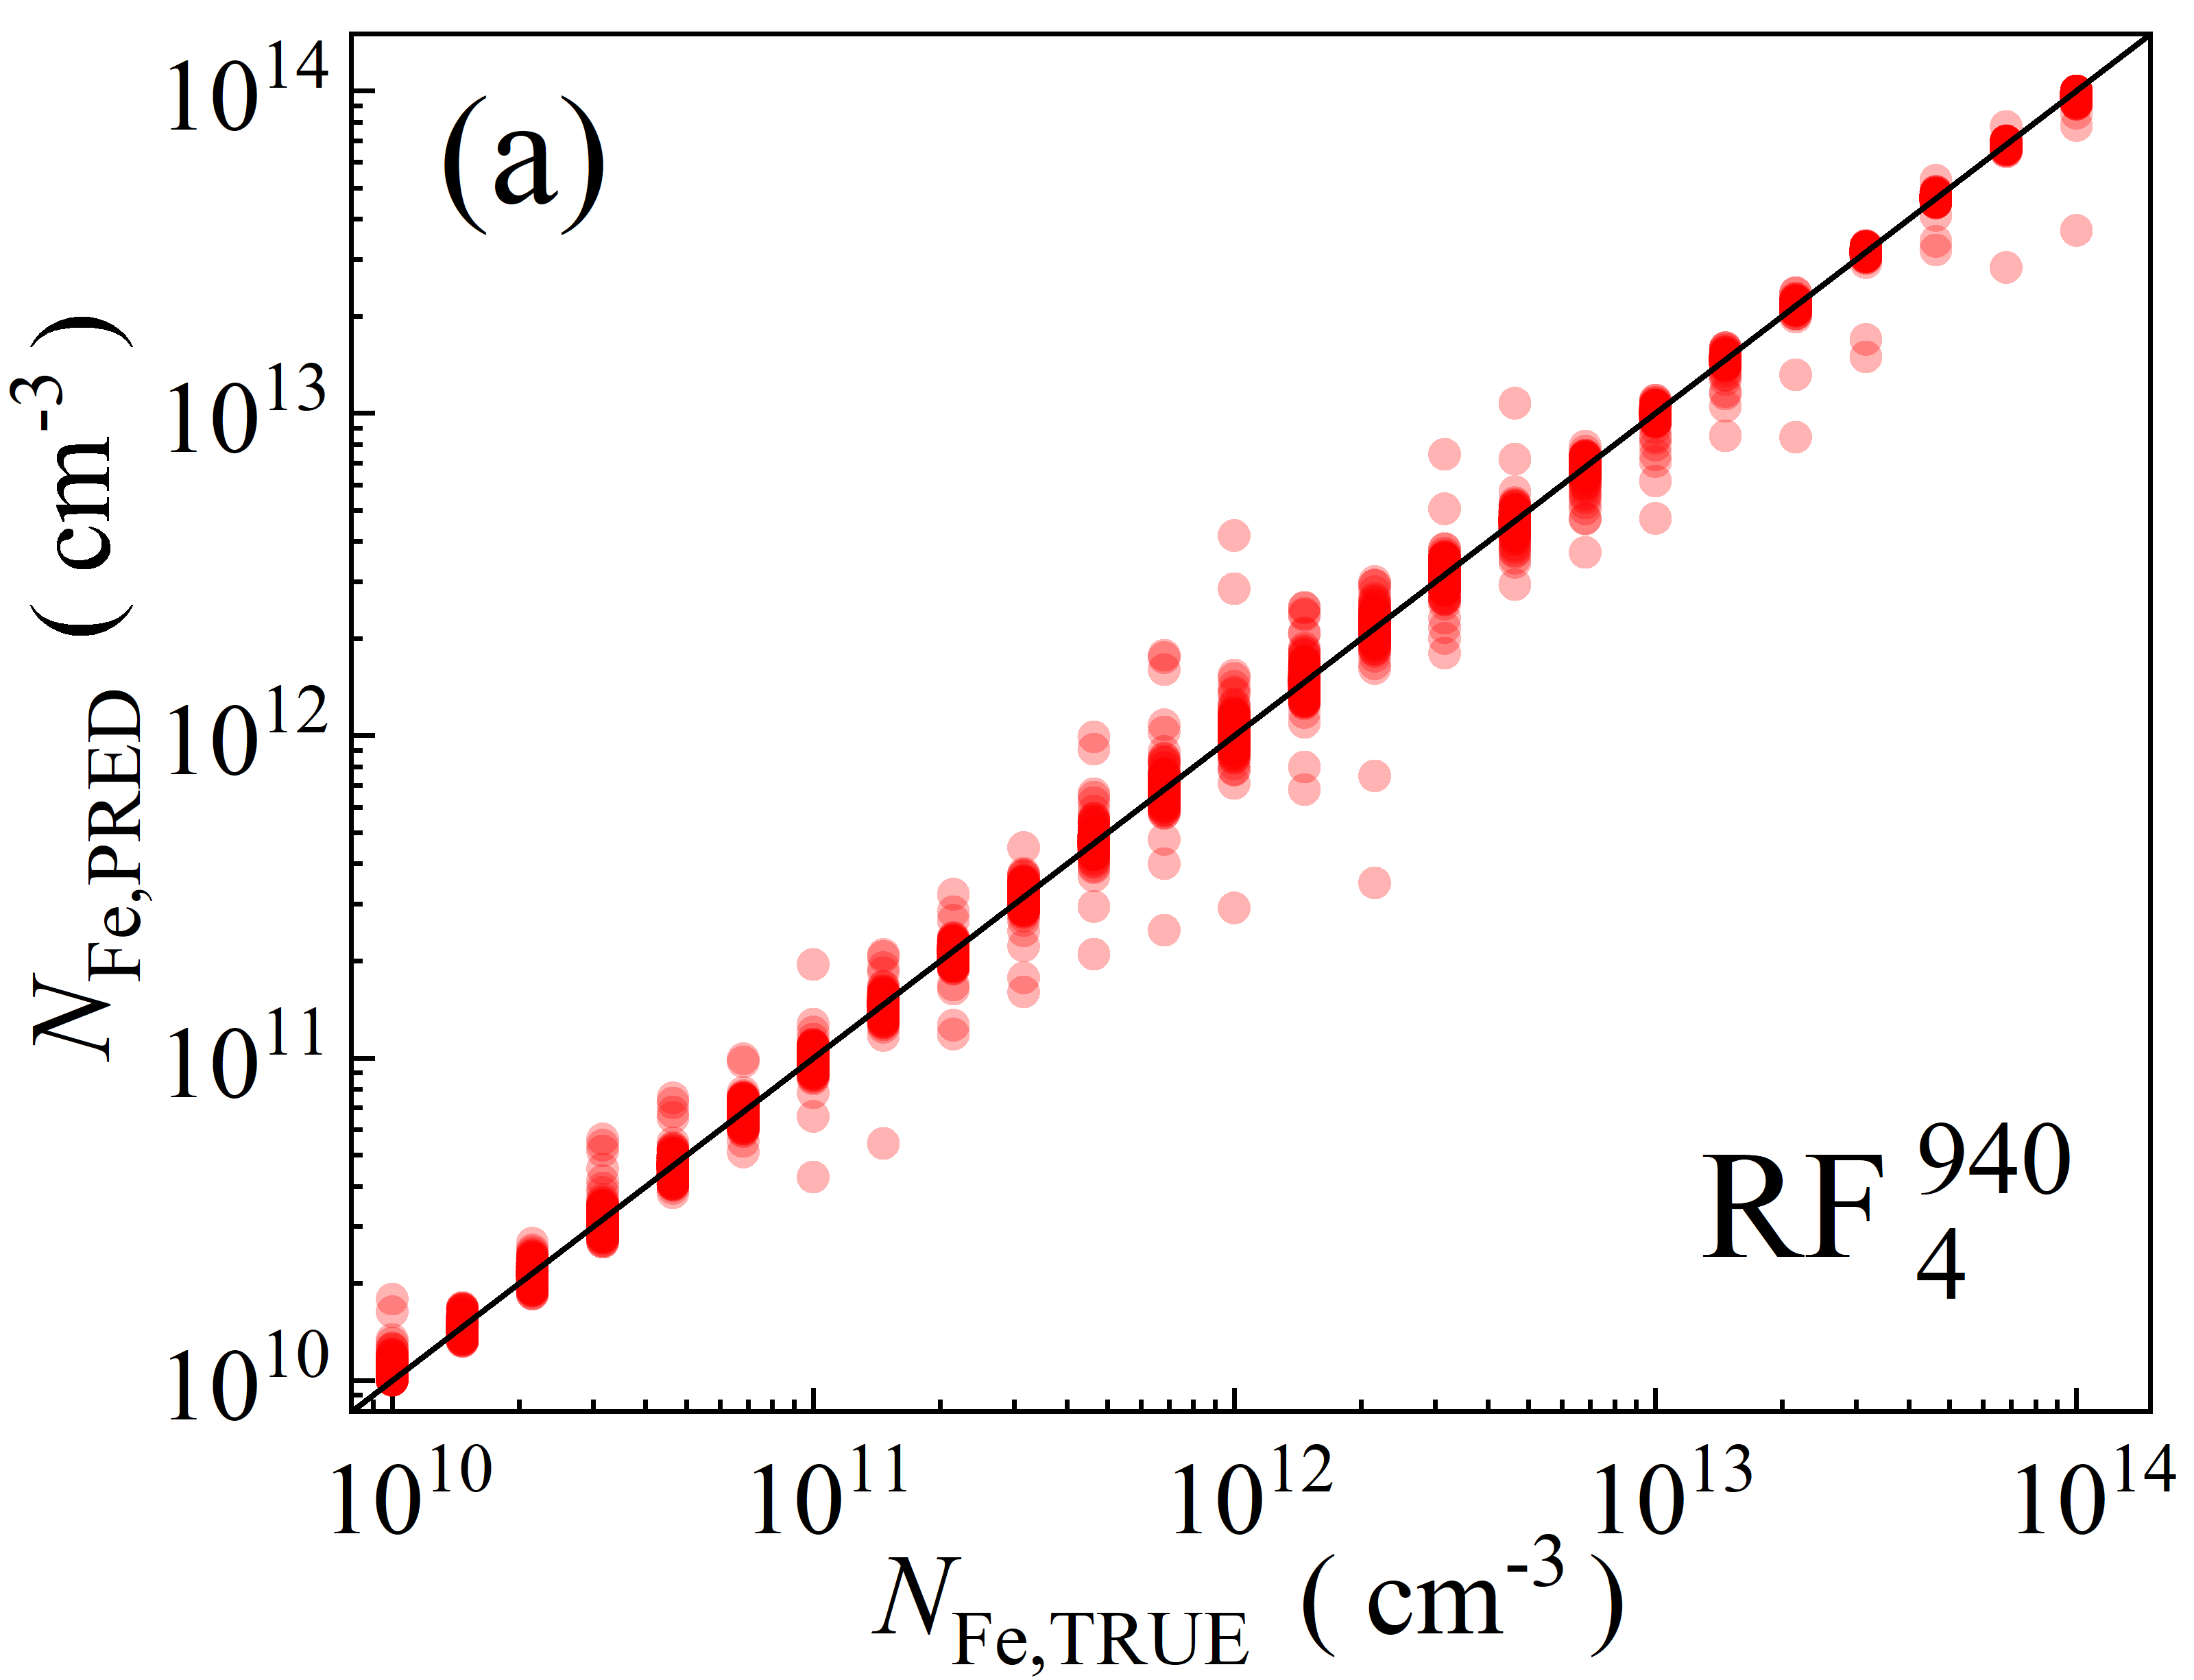
\includegraphics[width=0.24\linewidth]{Fig3a.png}
     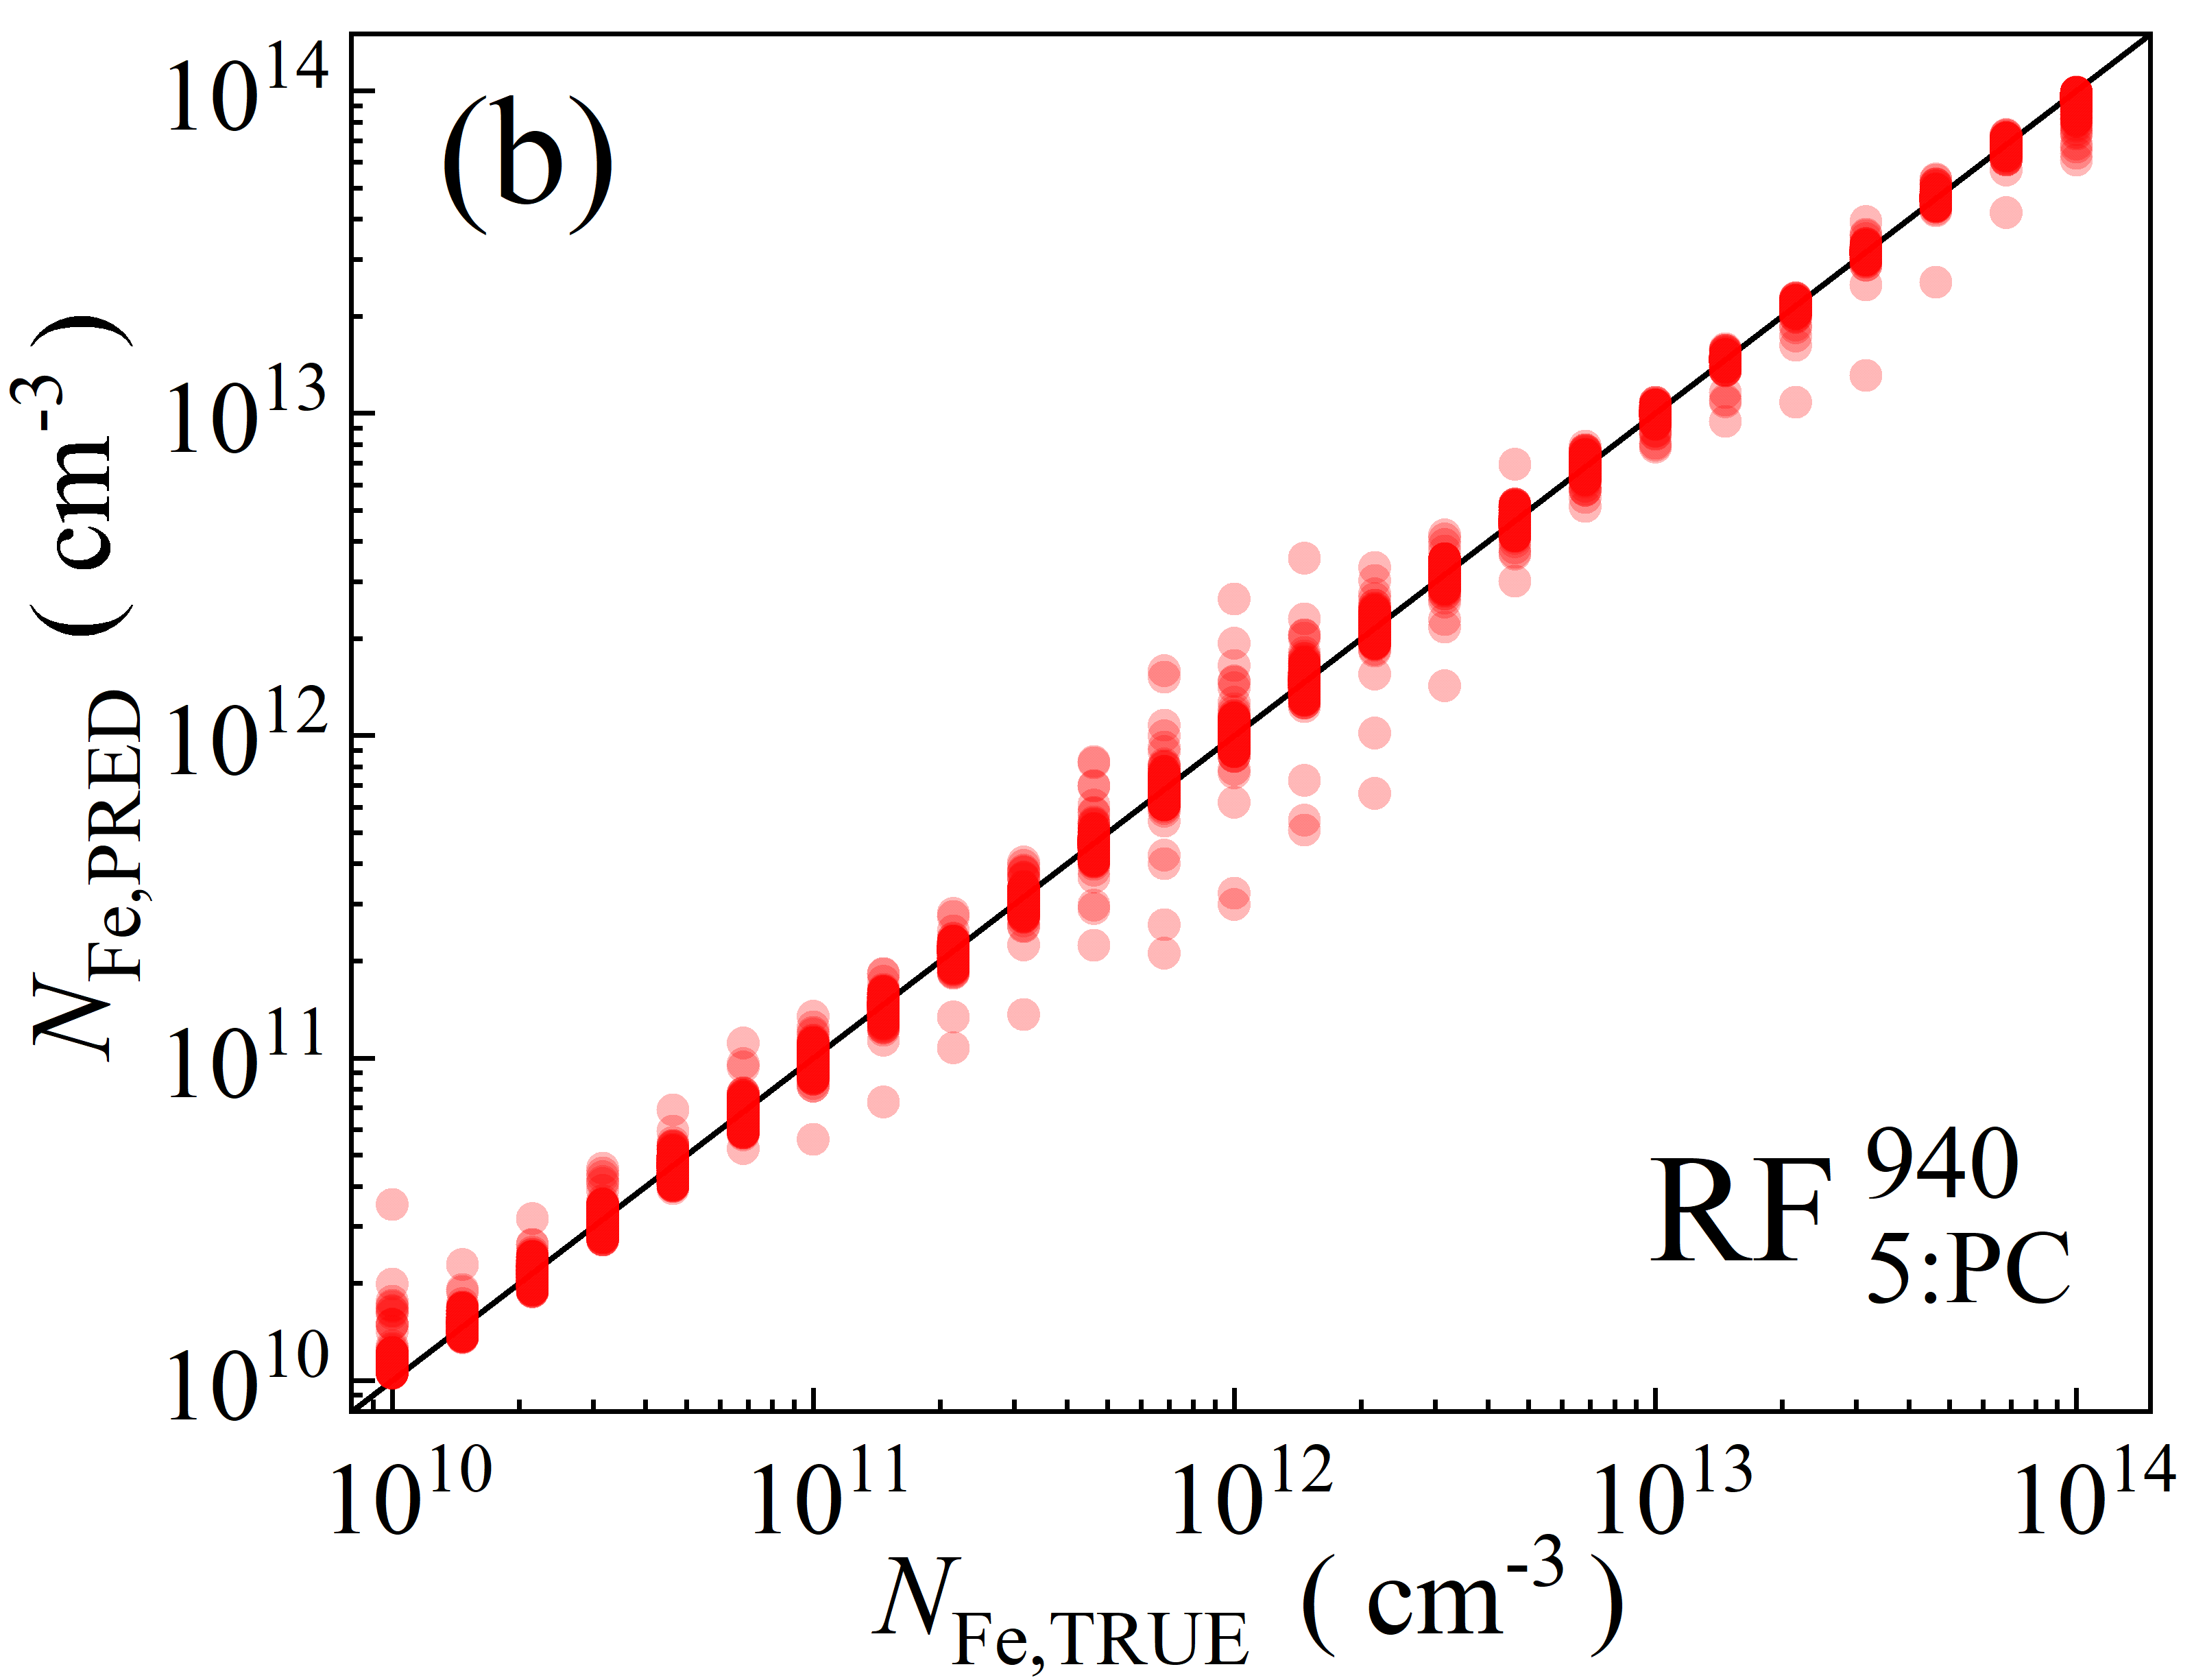
\includegraphics[width=0.24\linewidth]{Fig3b.png}
     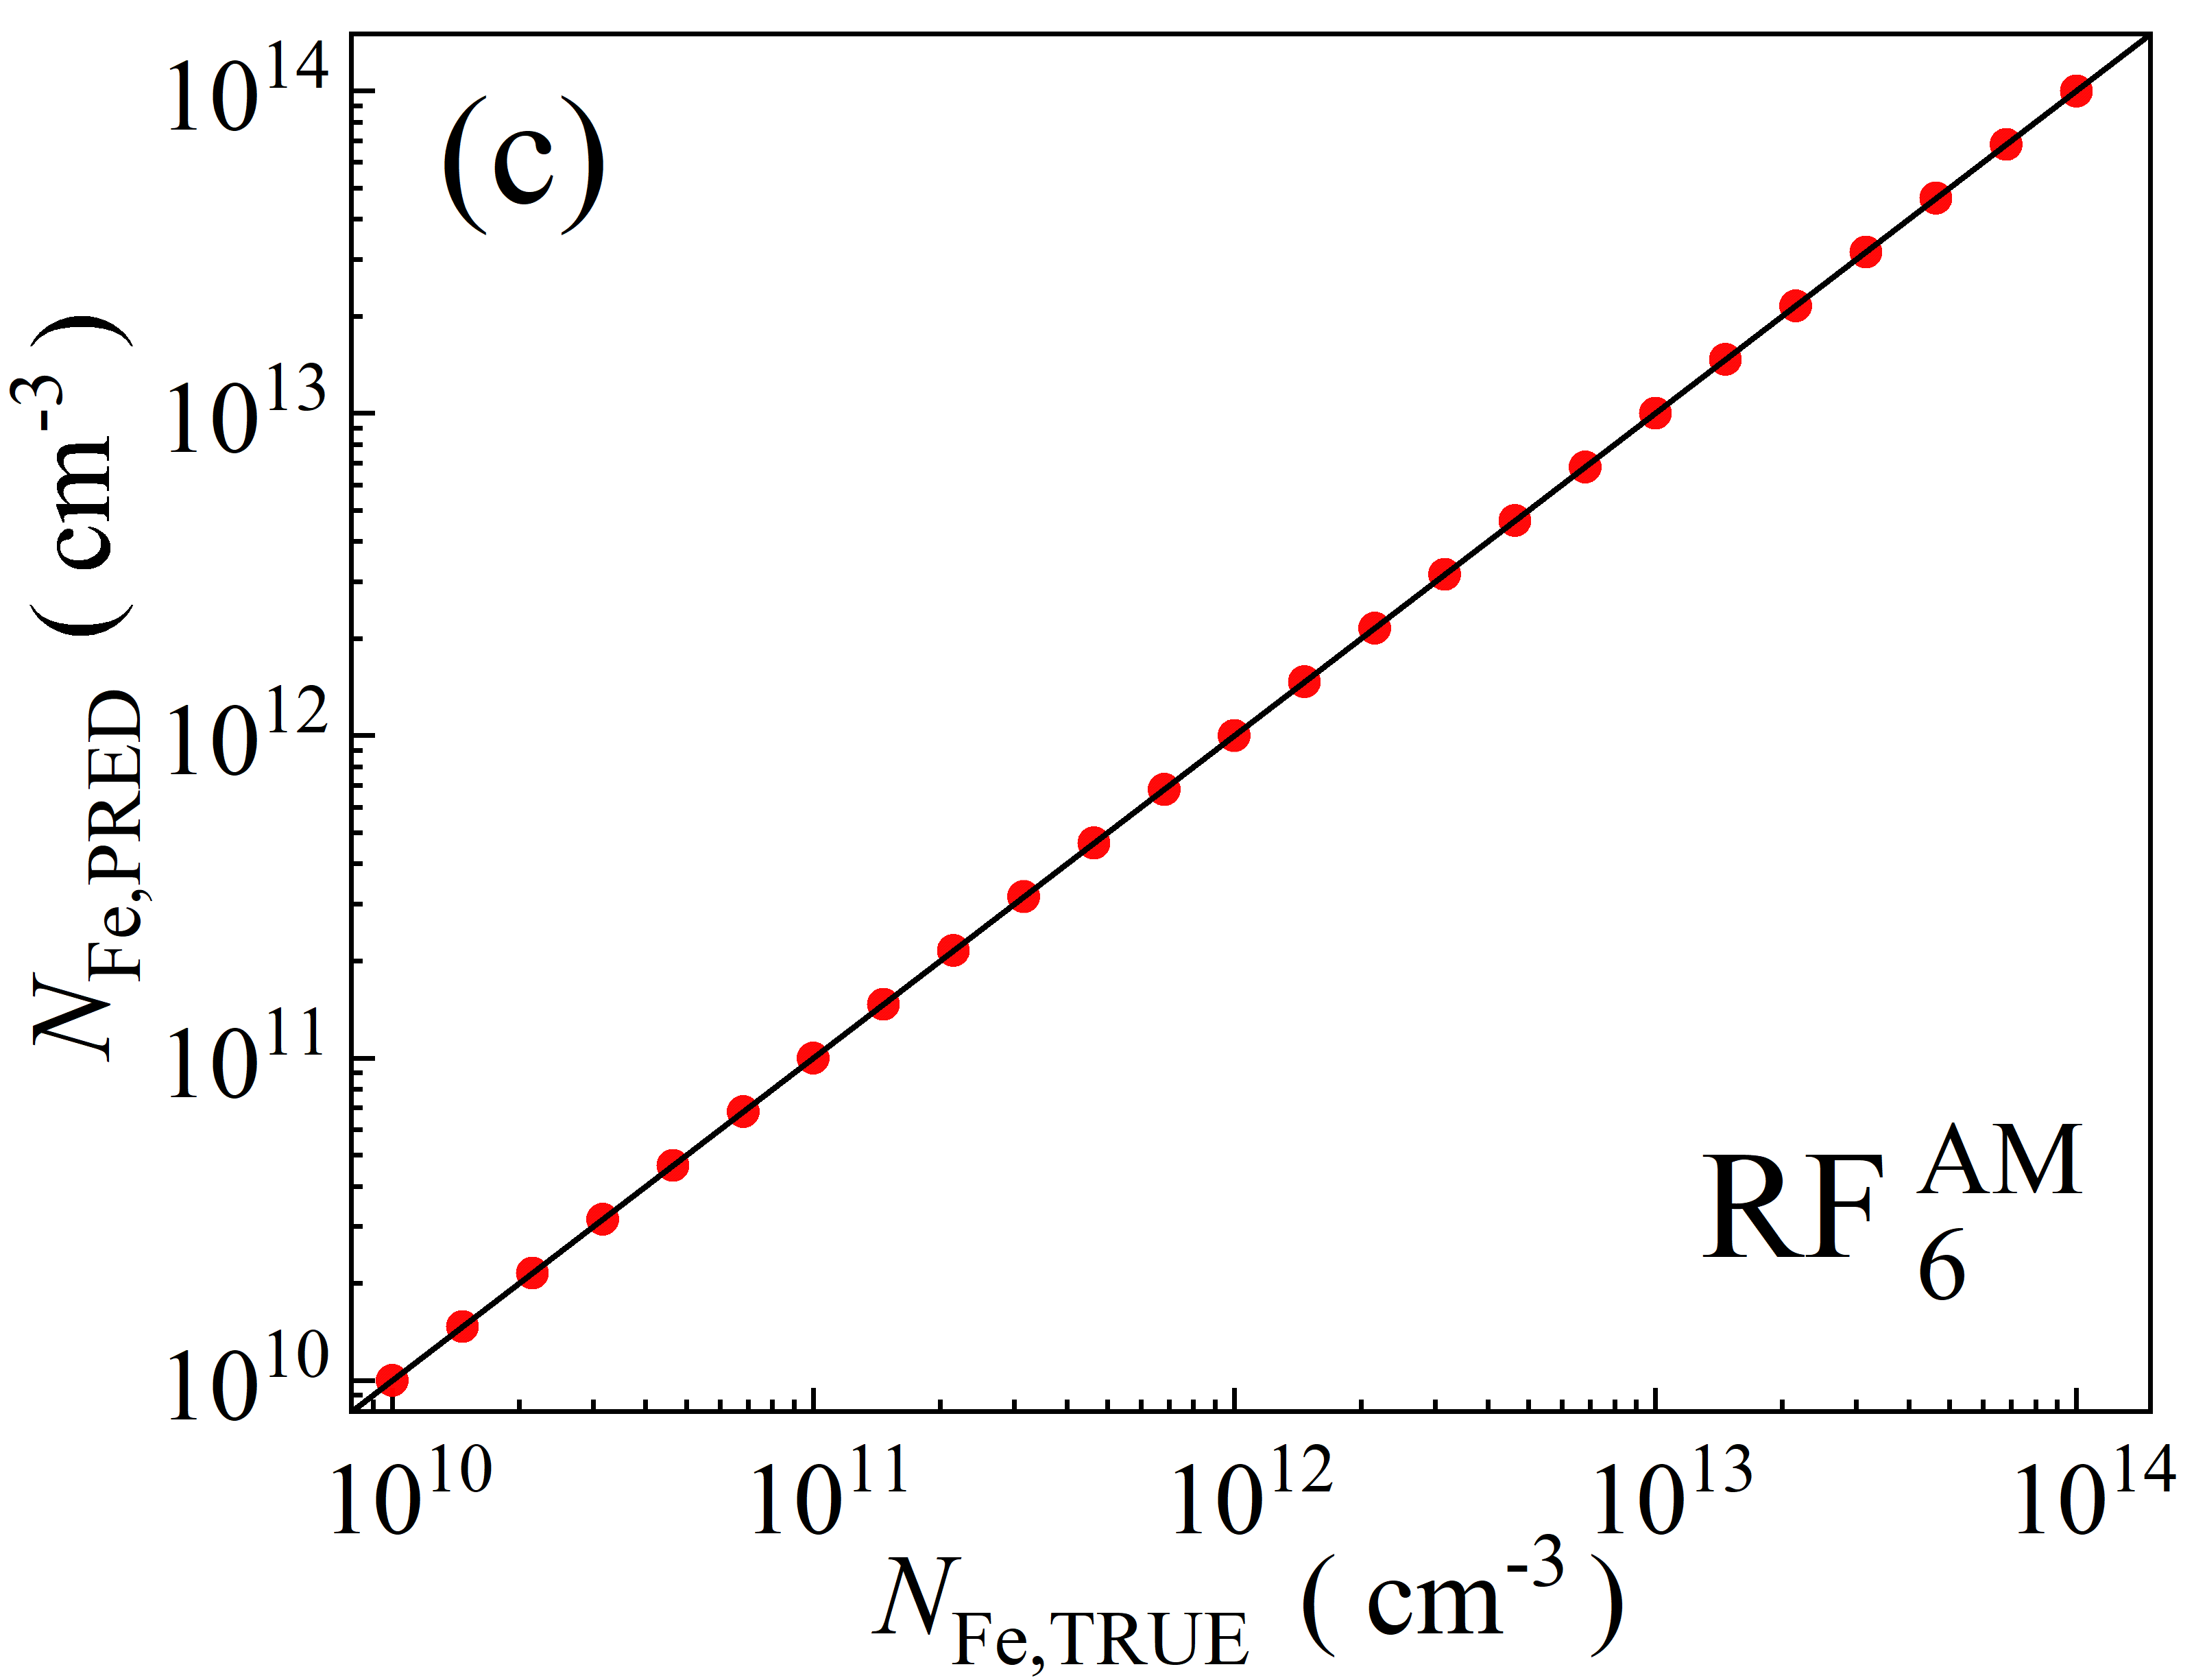
\includegraphics[width=0.24\linewidth]{Fig3c.png}
     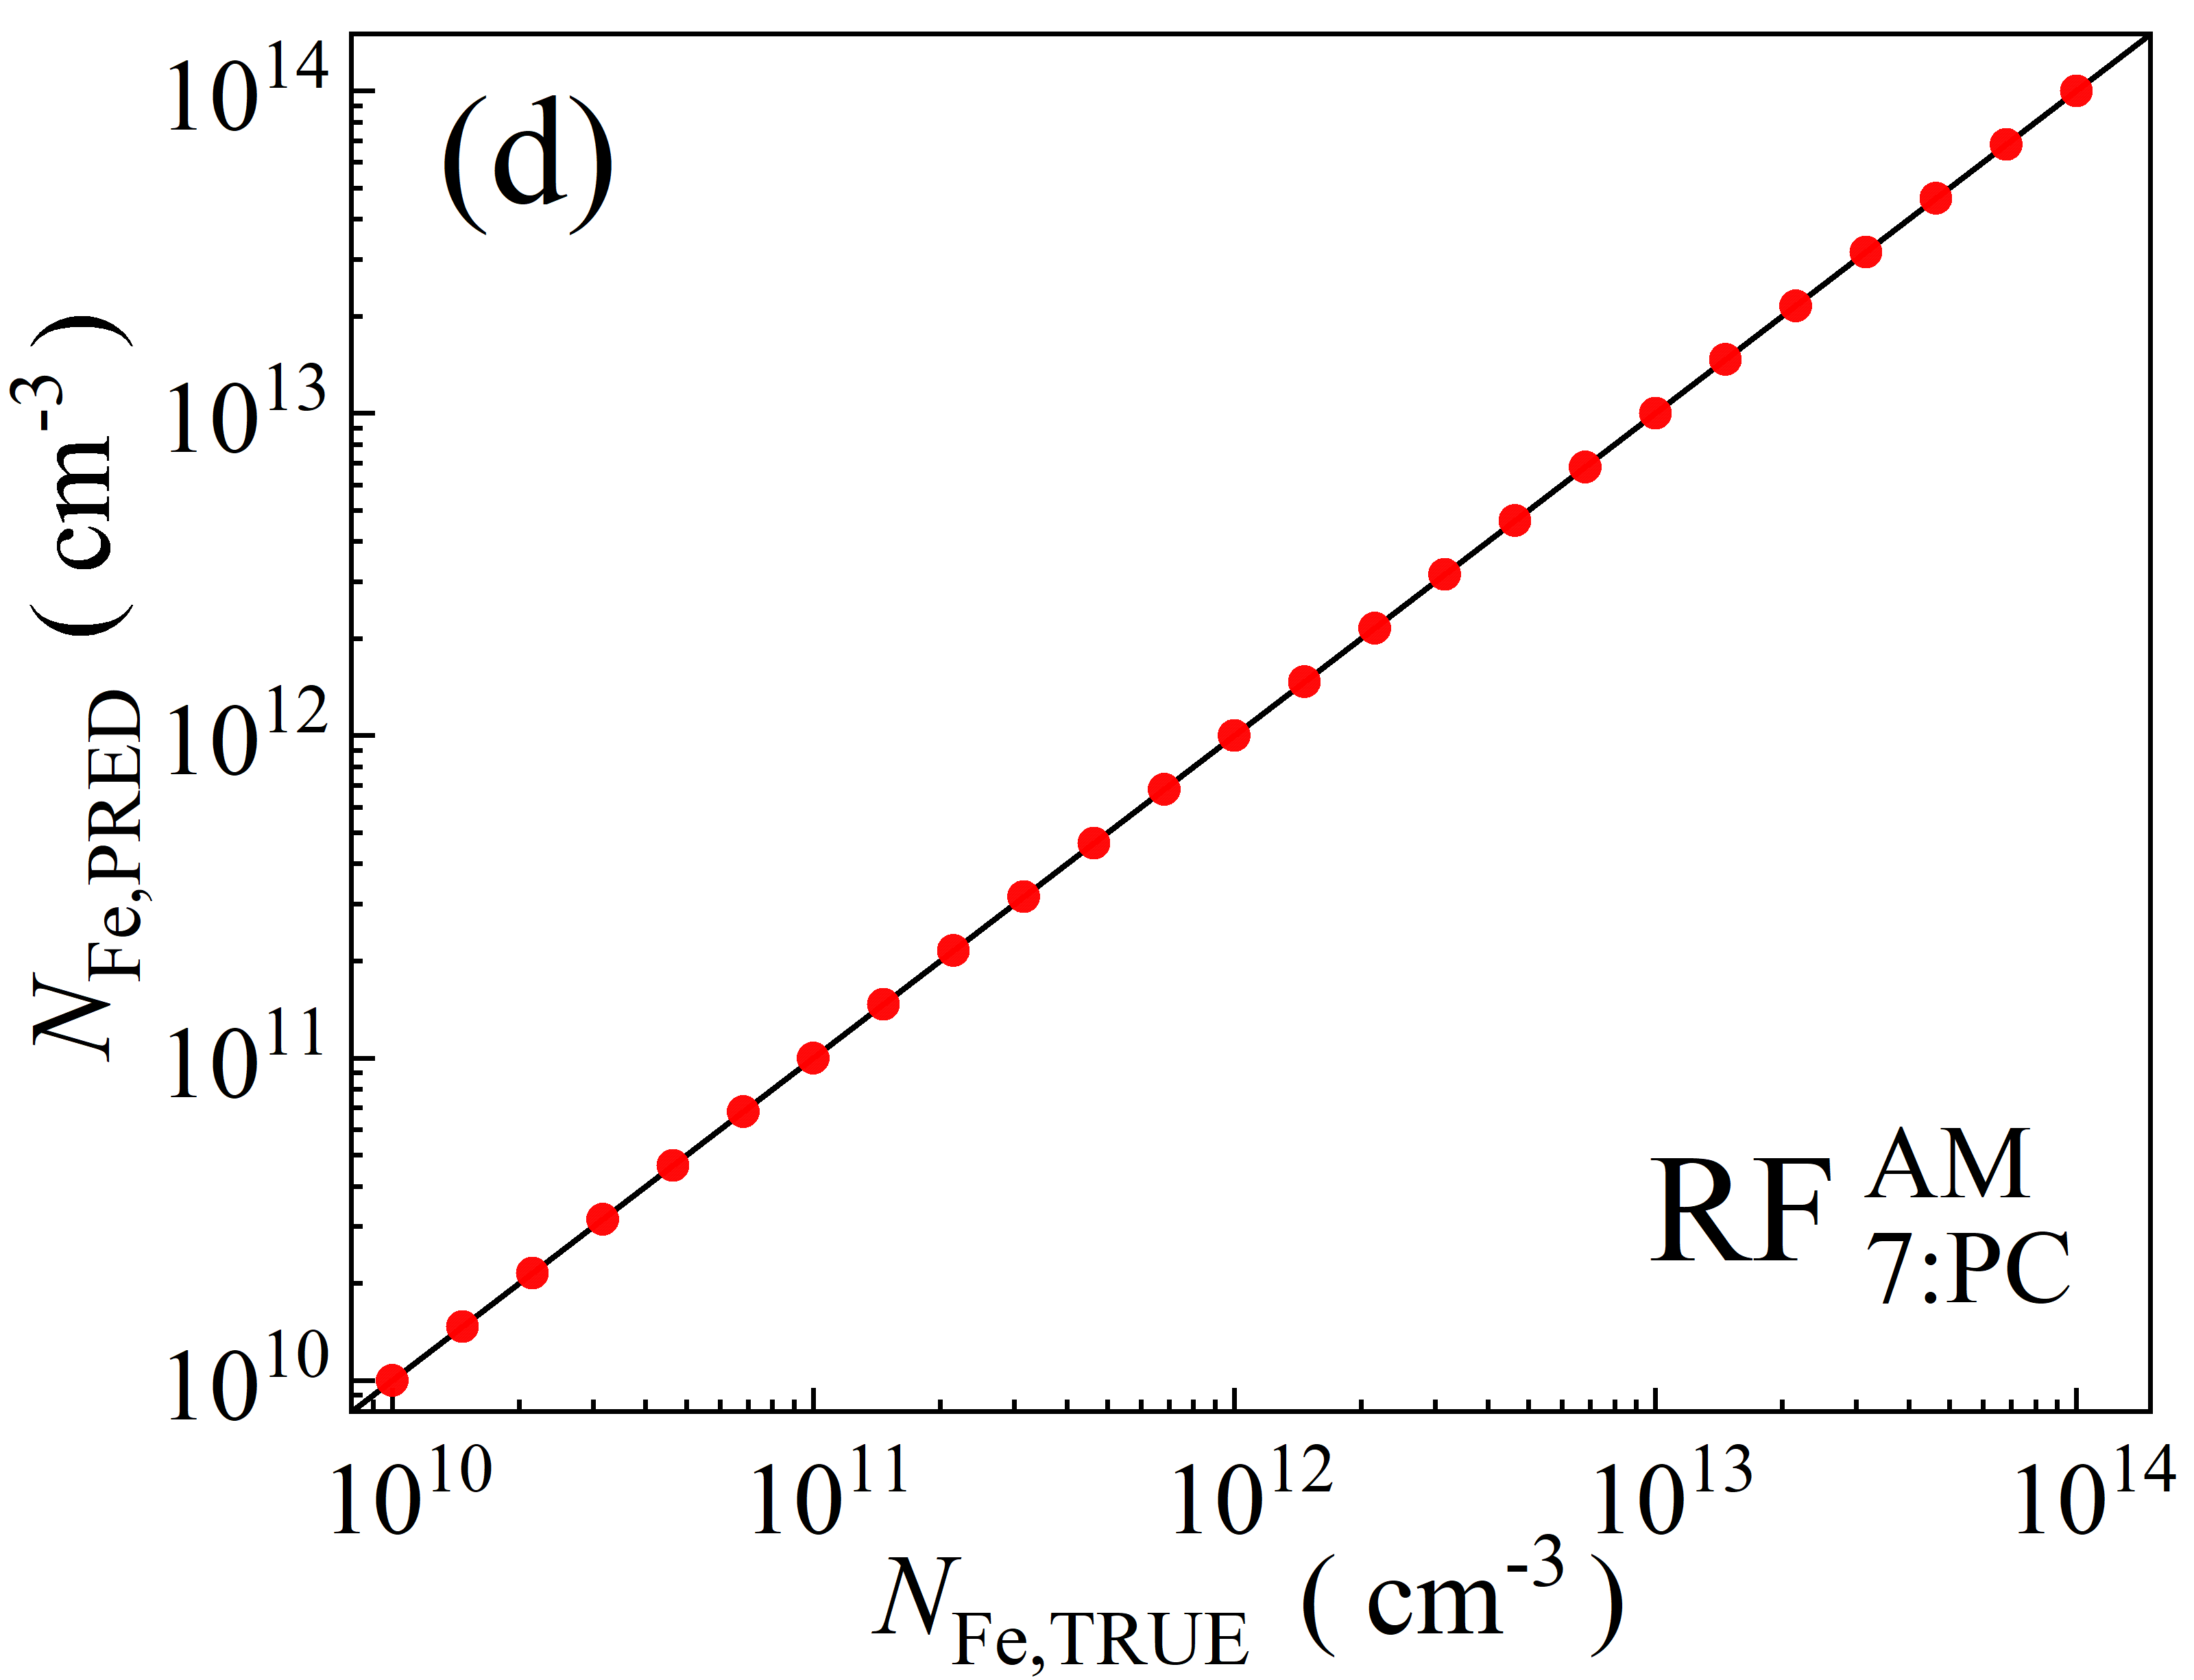
\includegraphics[width=0.24\linewidth]{Fig3d.png}
     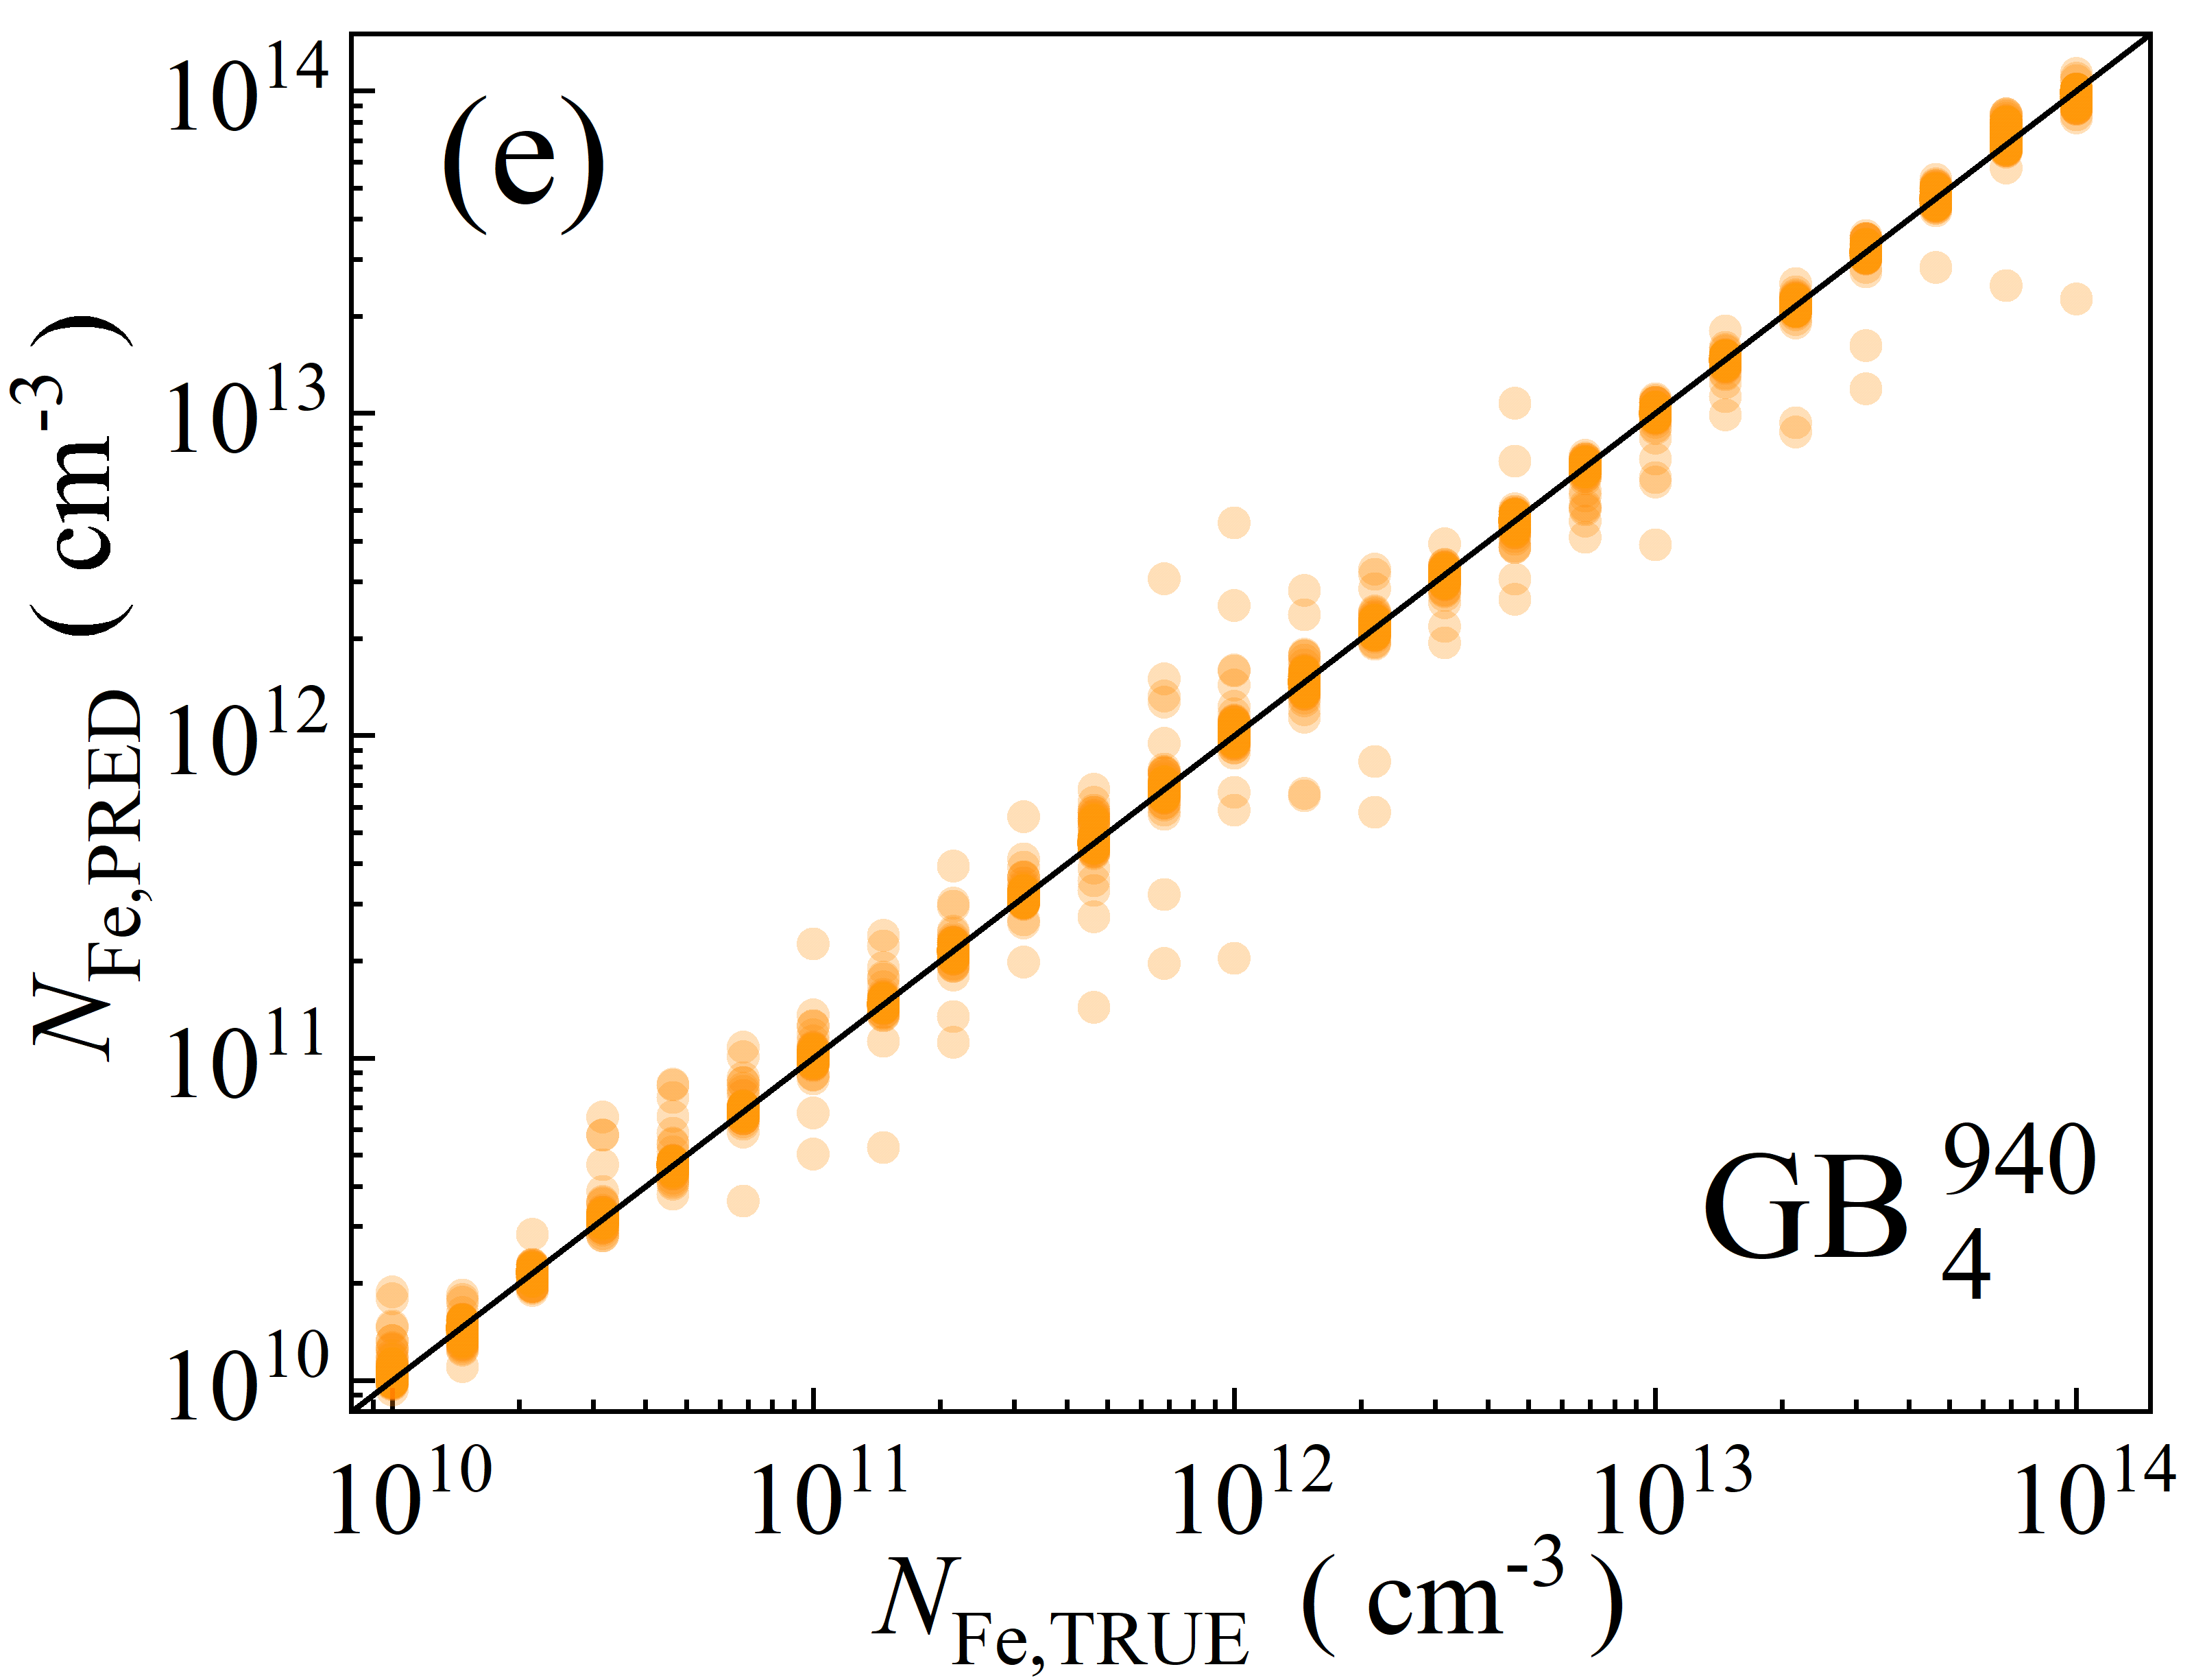
\includegraphics[width=0.24\linewidth]{Fig3e.png}
     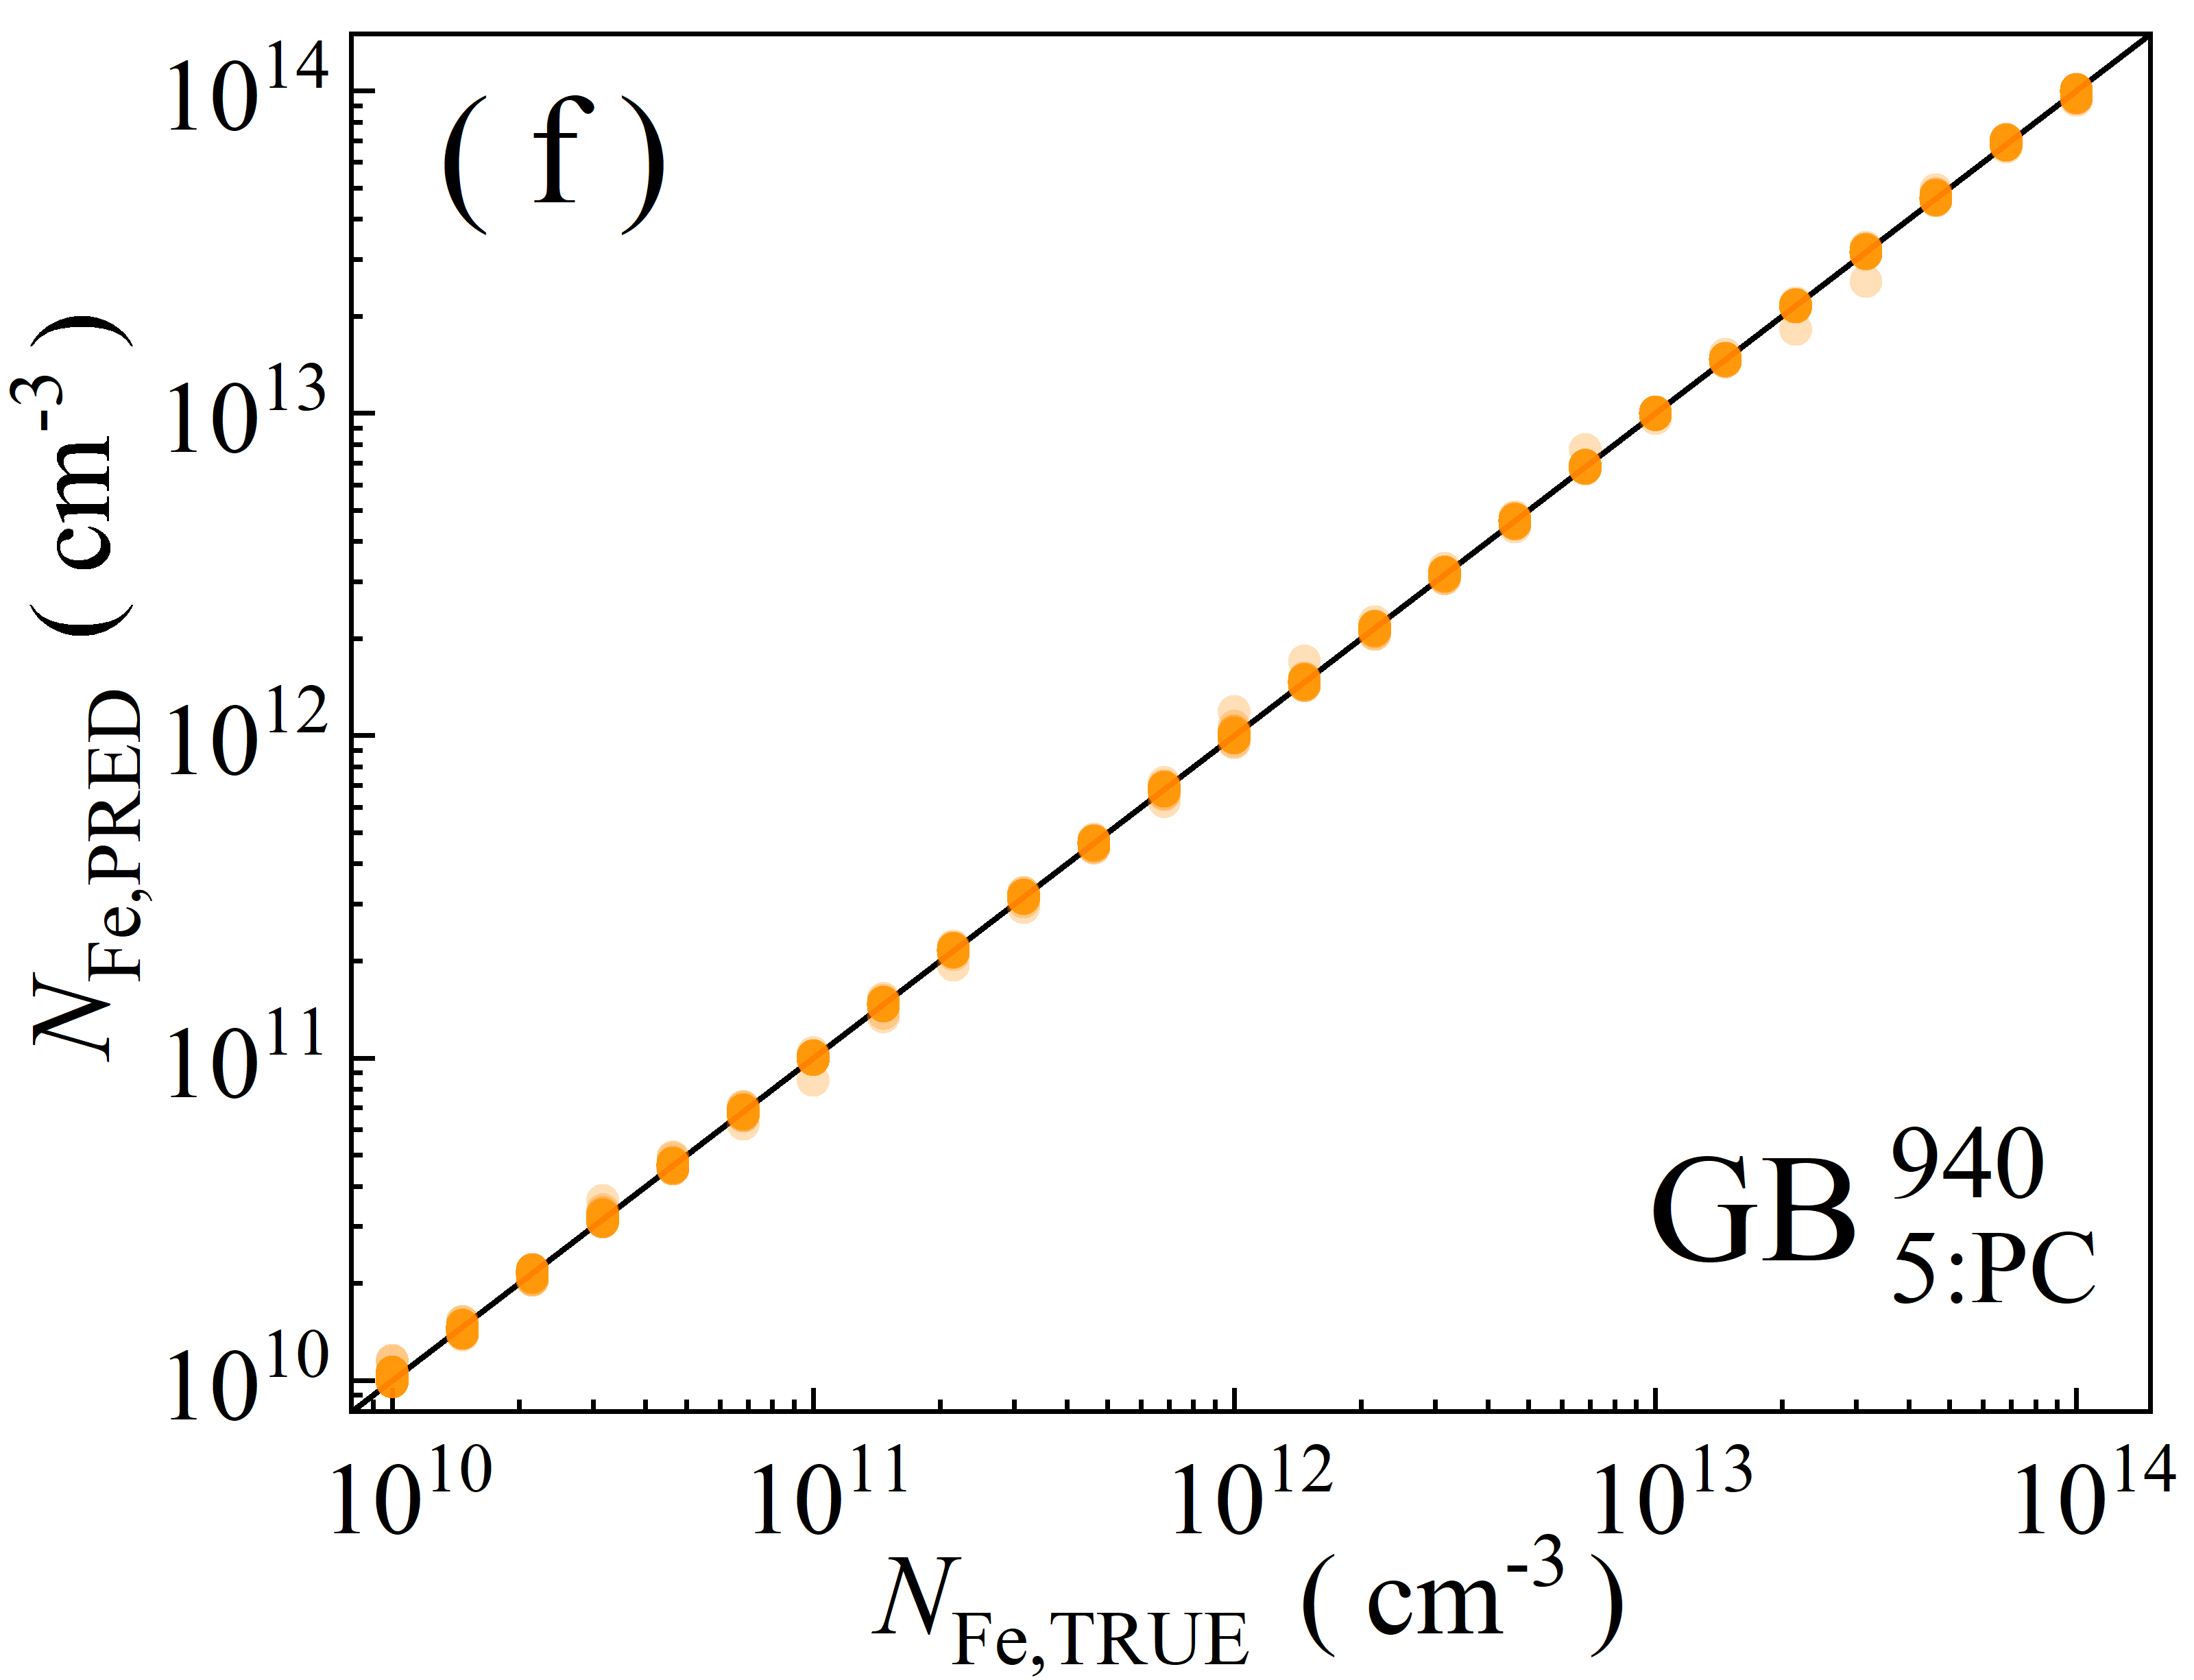
\includegraphics[width=0.24\linewidth]{Fig3f.png}
     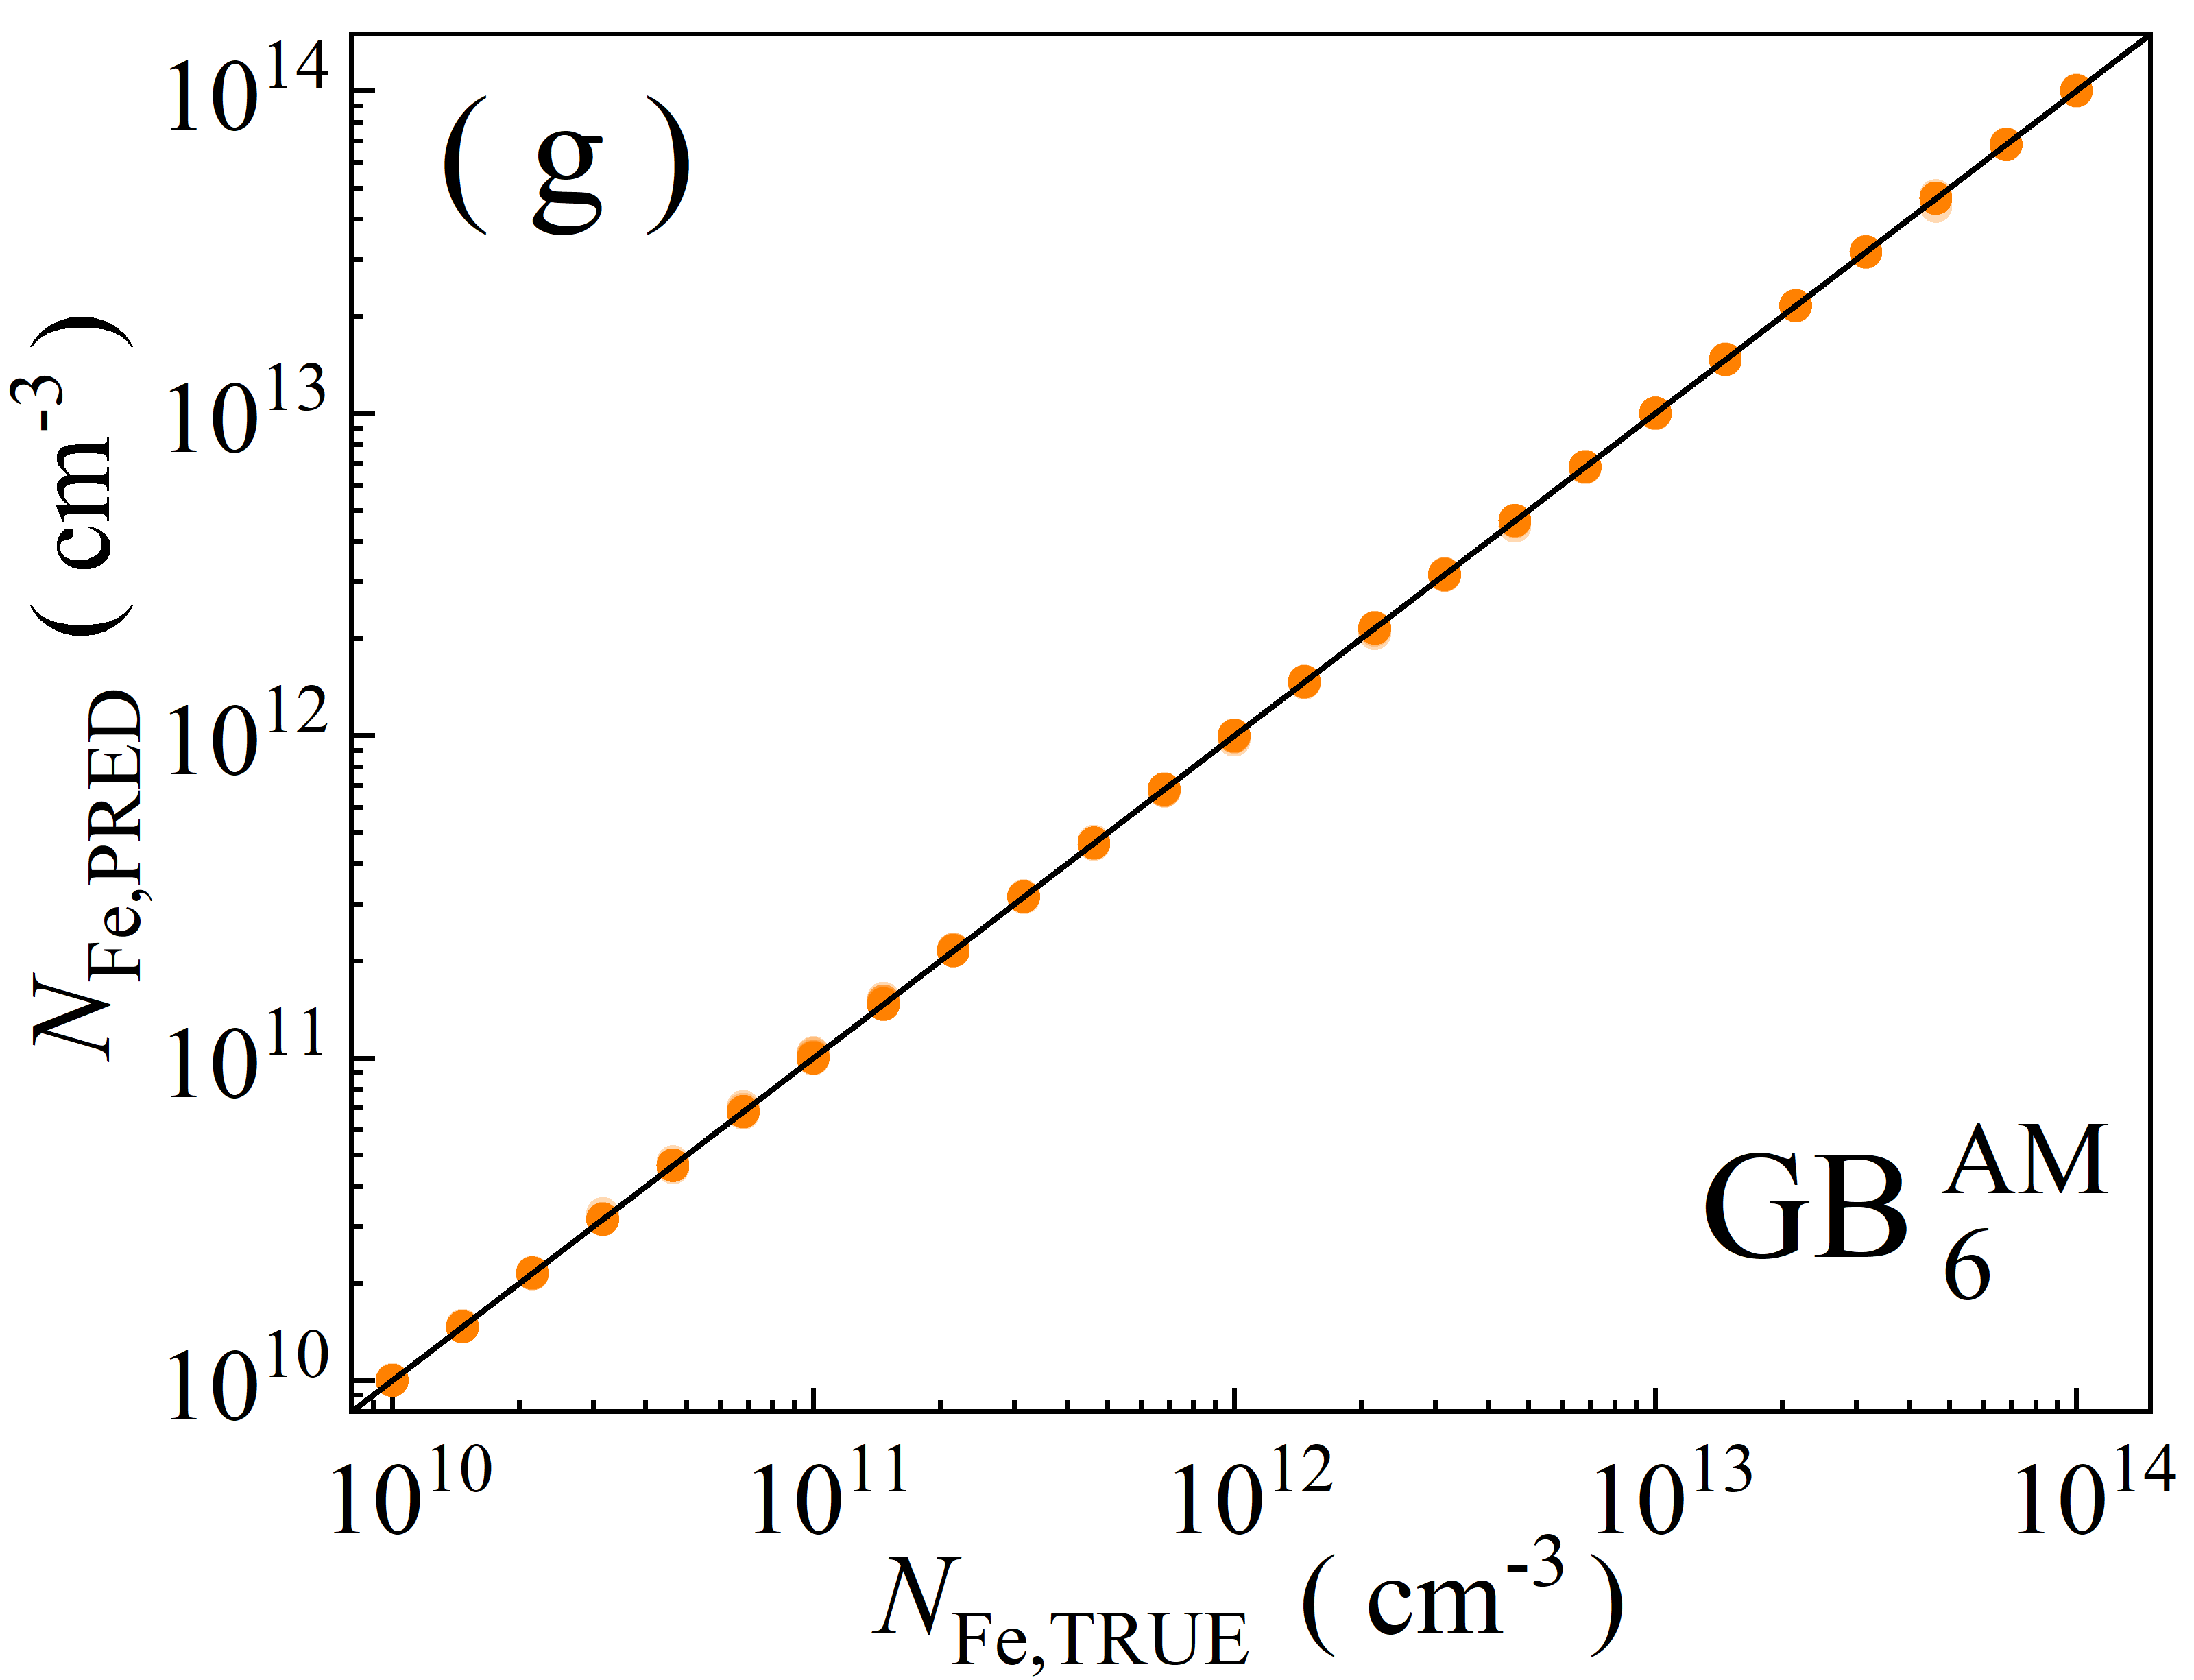
\includegraphics[width=0.24\linewidth]{Fig3g.png}
     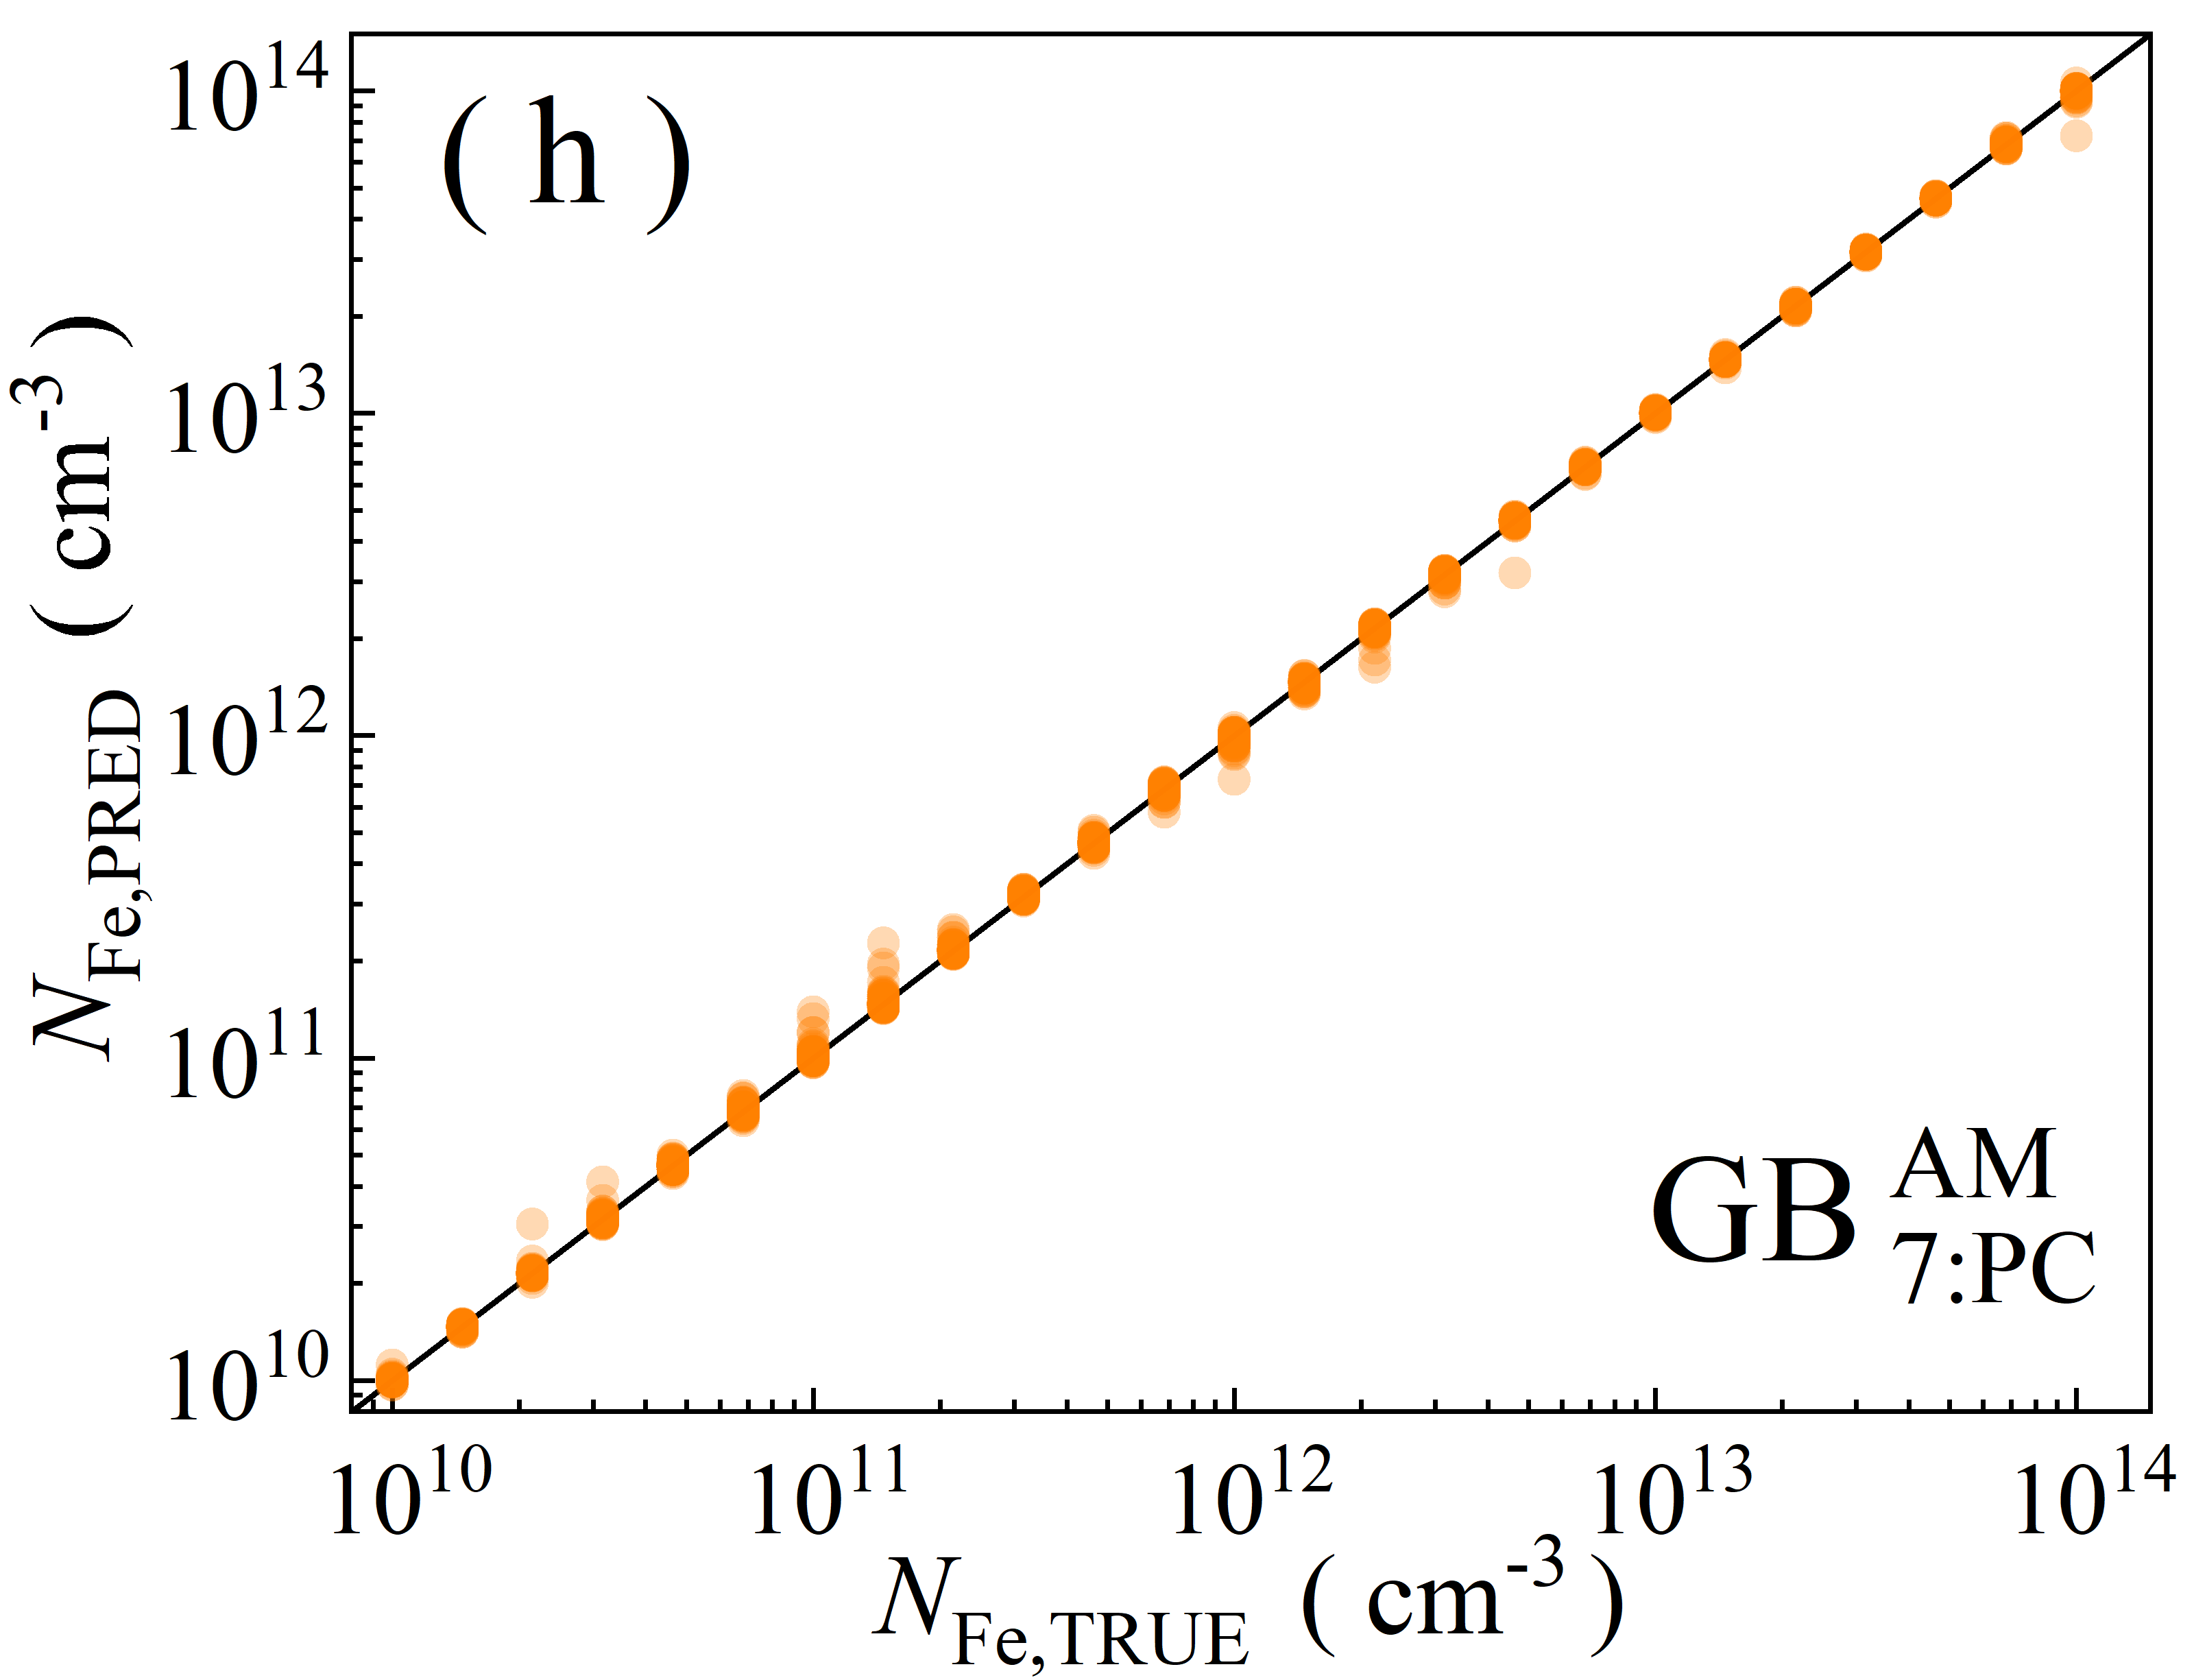
\includegraphics[width=0.24\linewidth]{Fig3h.png}
     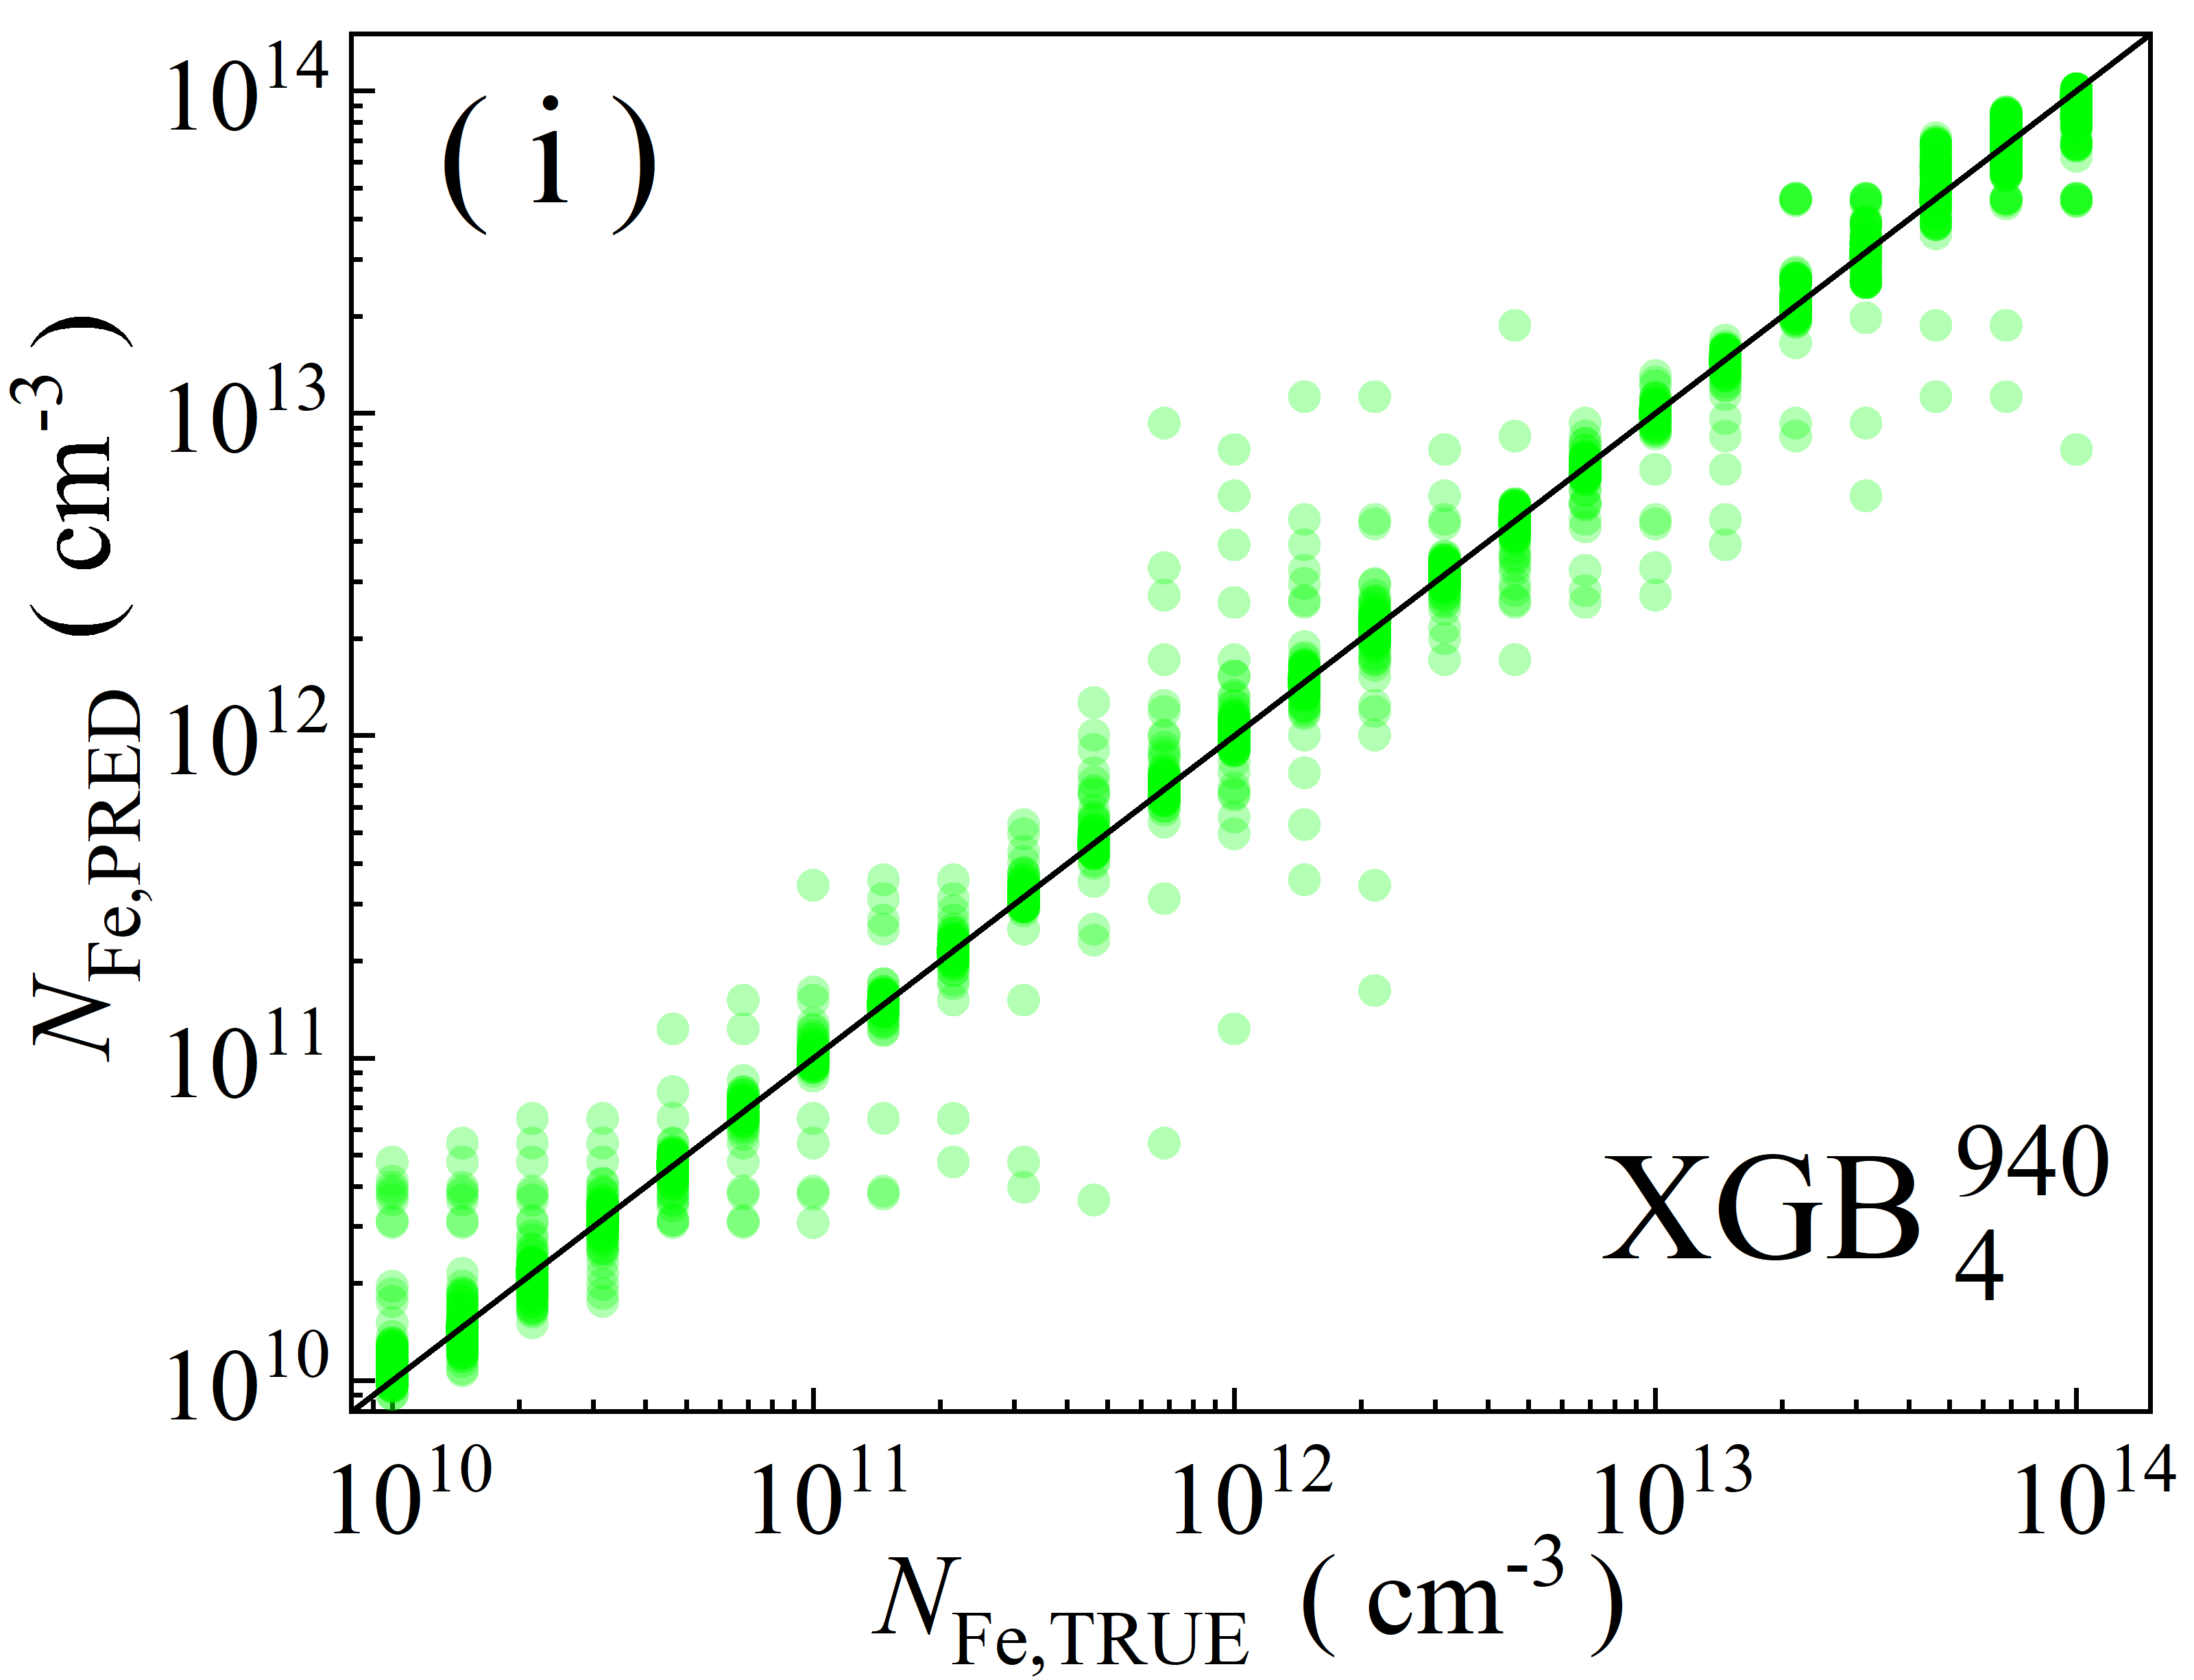
\includegraphics[width=0.24\linewidth]{Fig3i.png}
     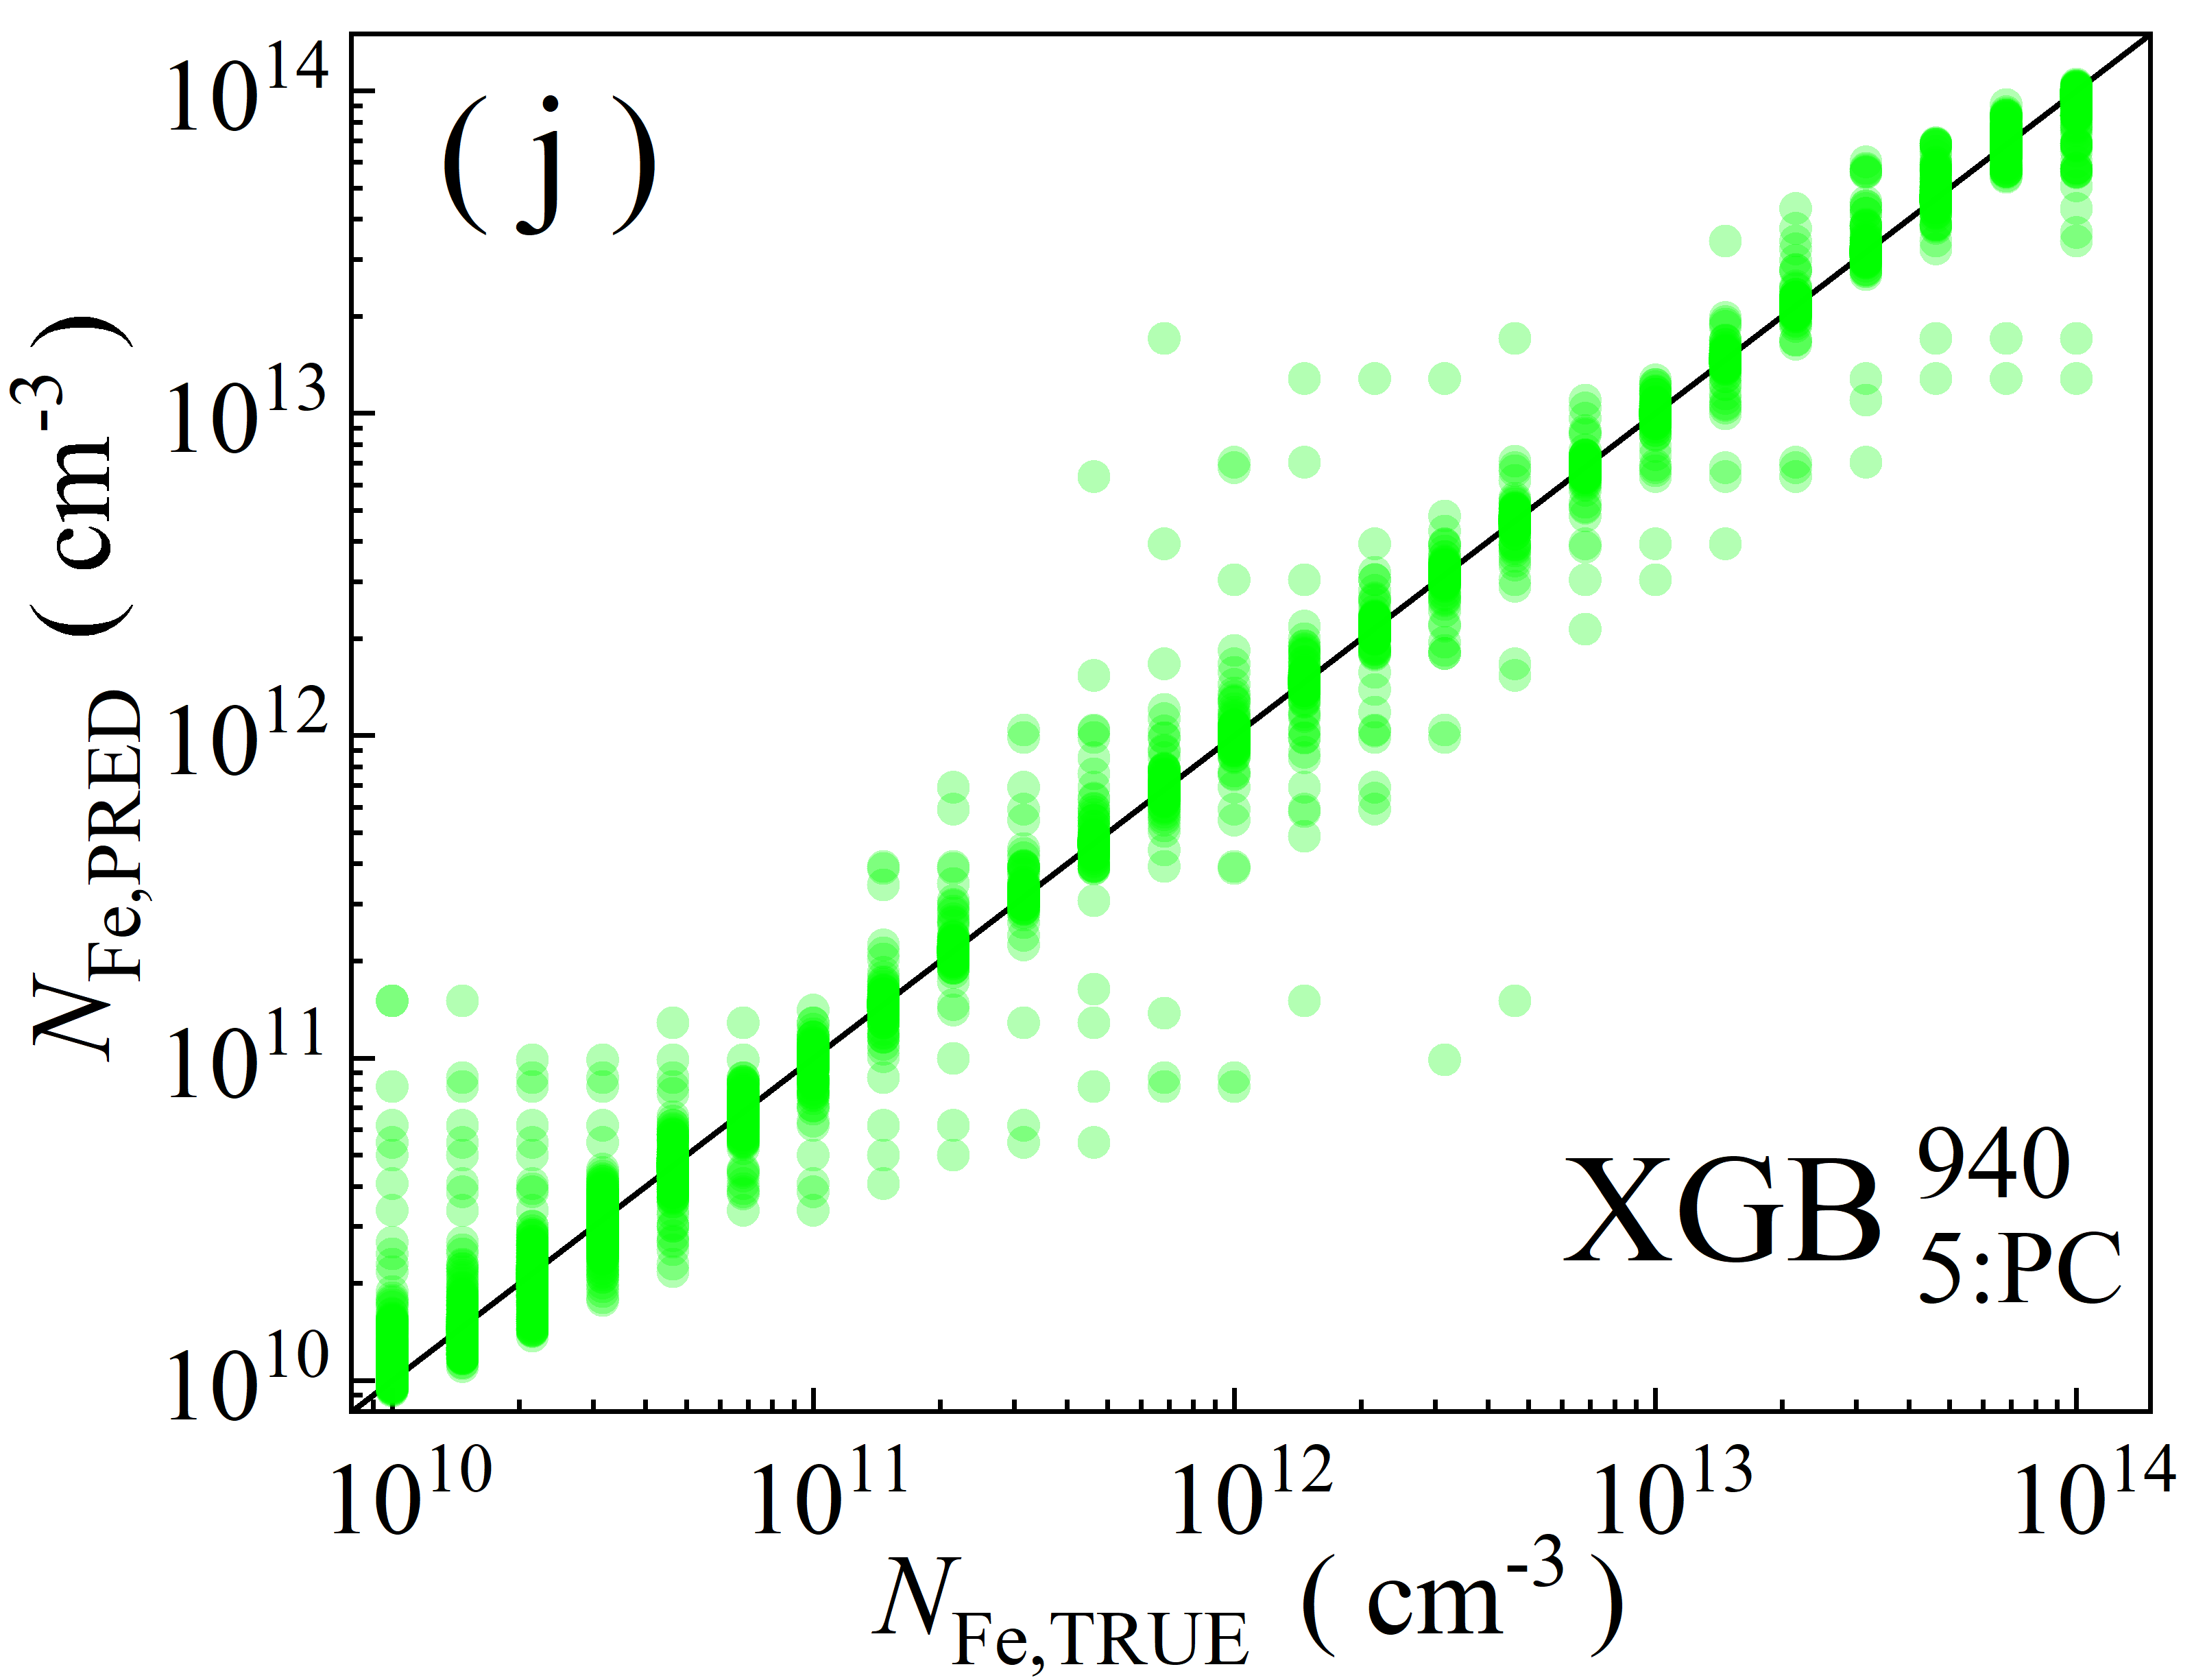
\includegraphics[width=0.24\linewidth]{Fig3j.png}
     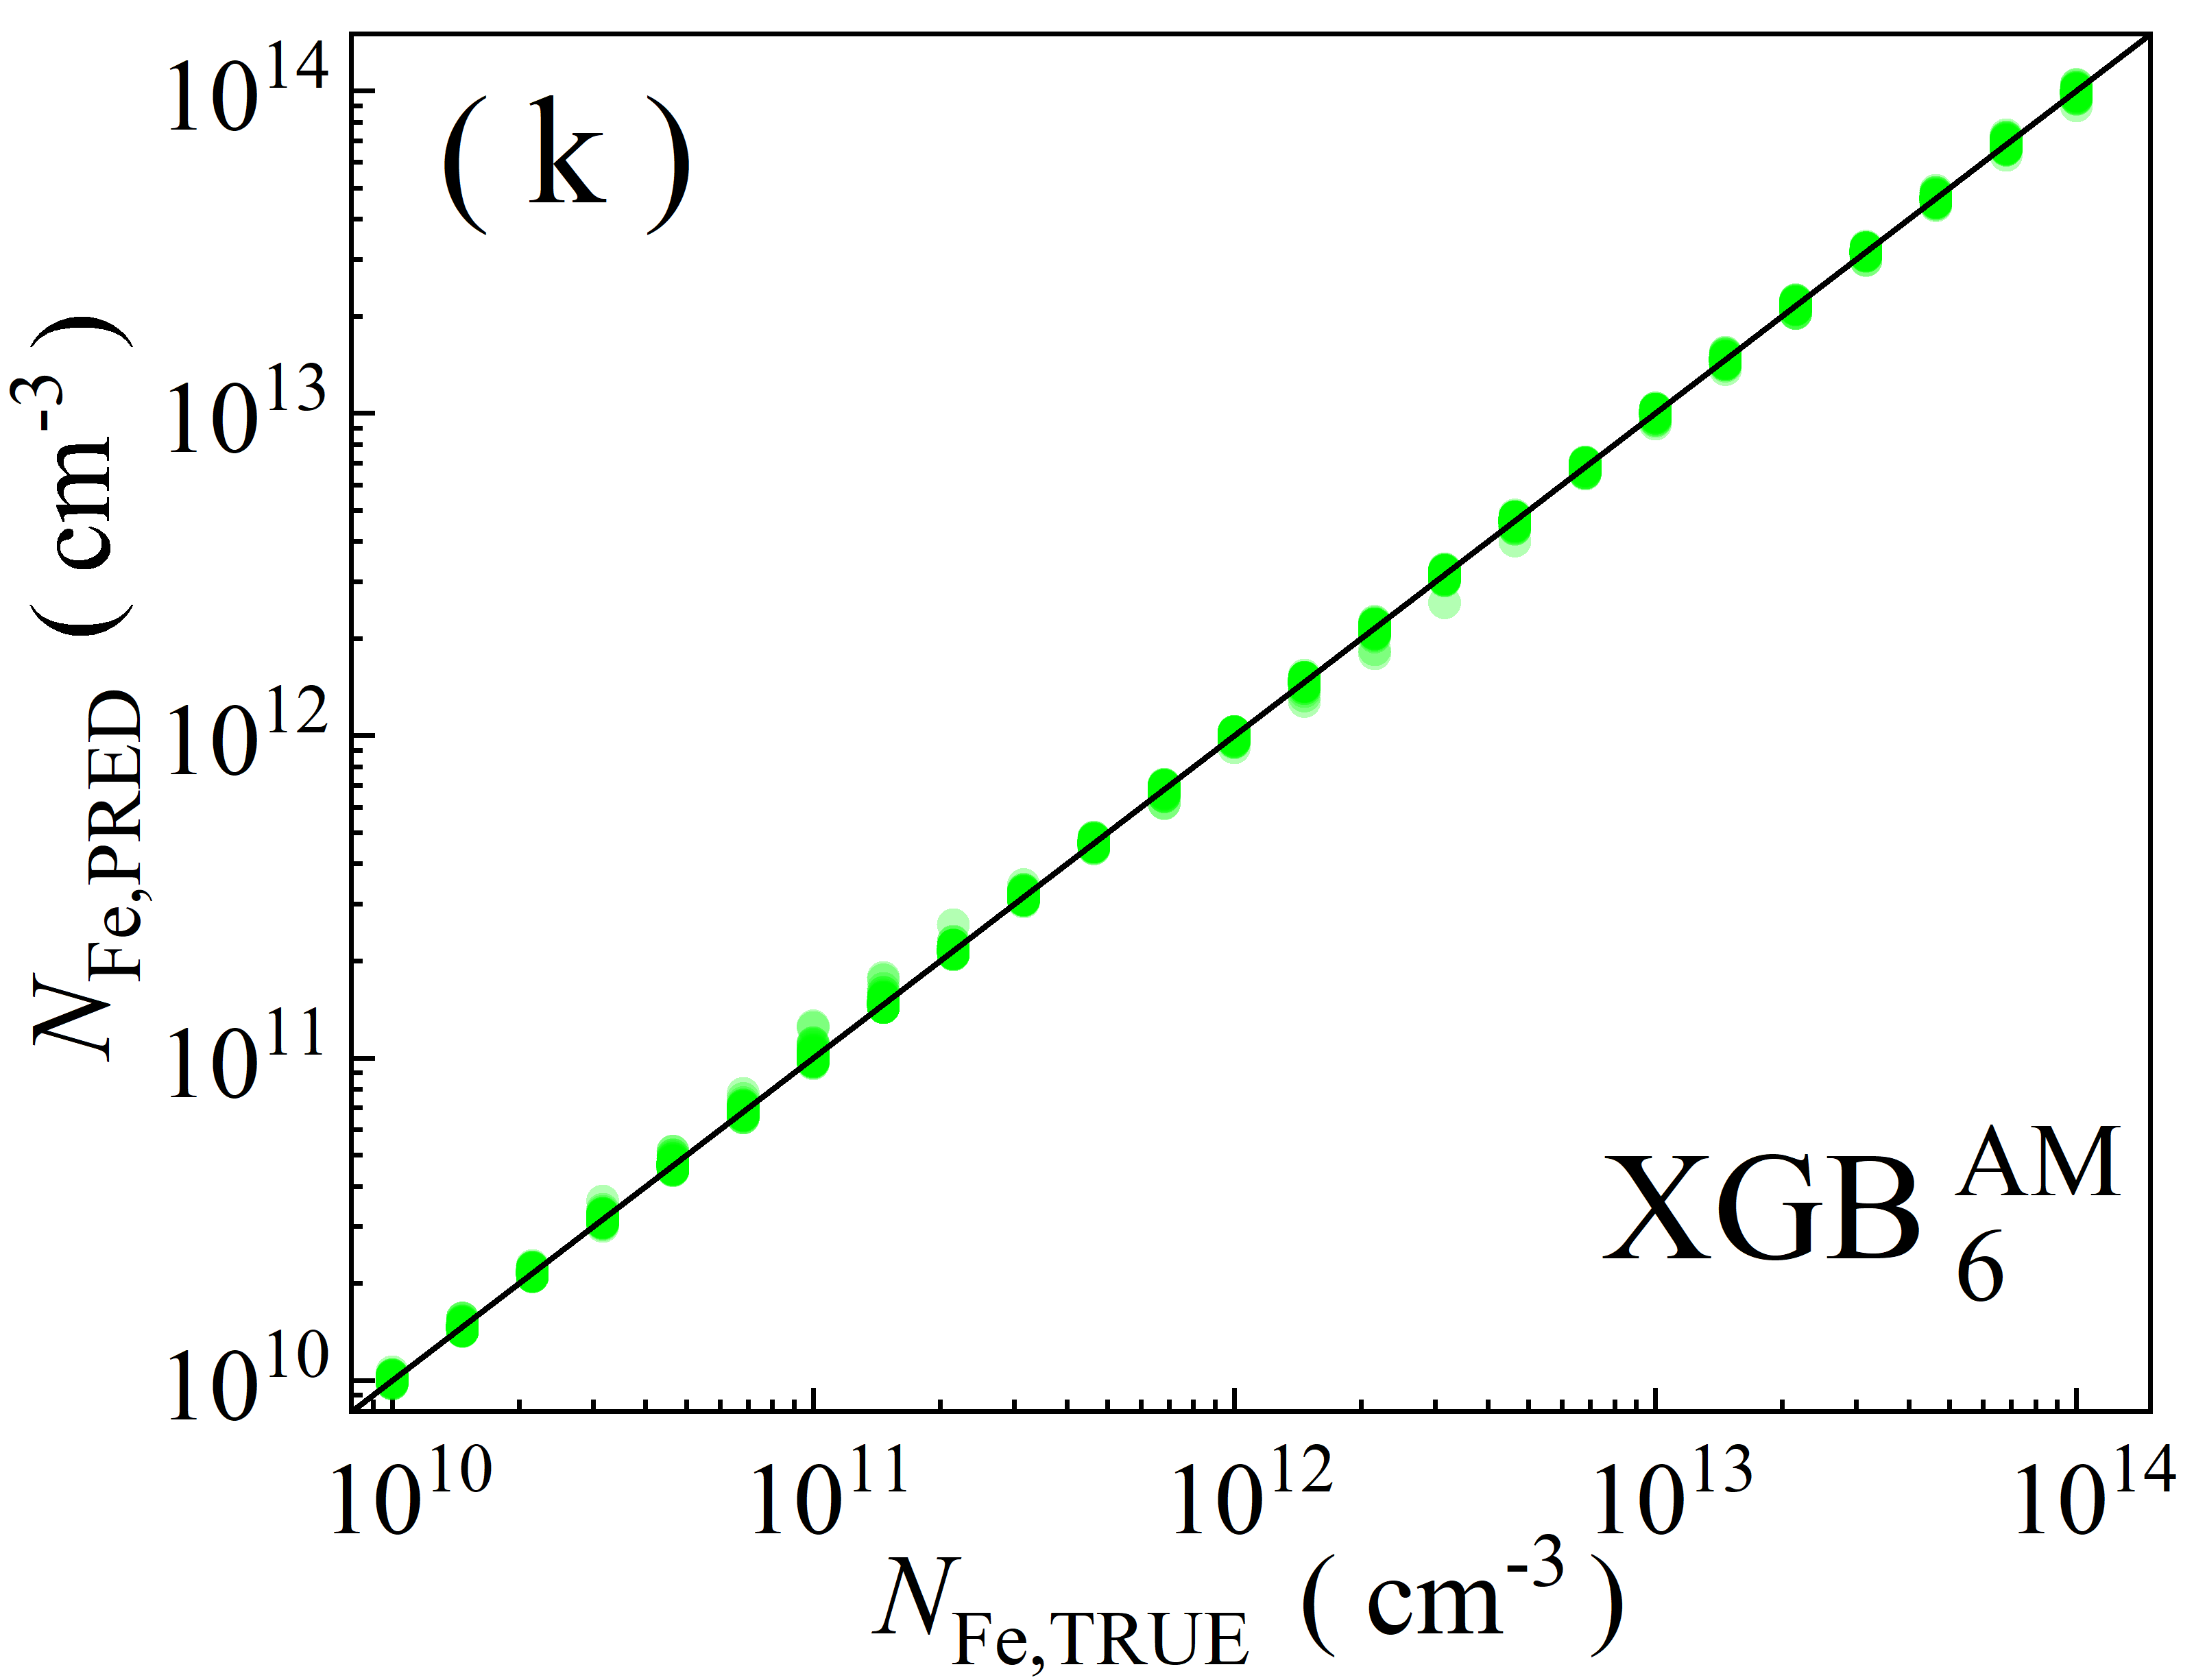
\includegraphics[width=0.24\linewidth]{Fig3k.png}
     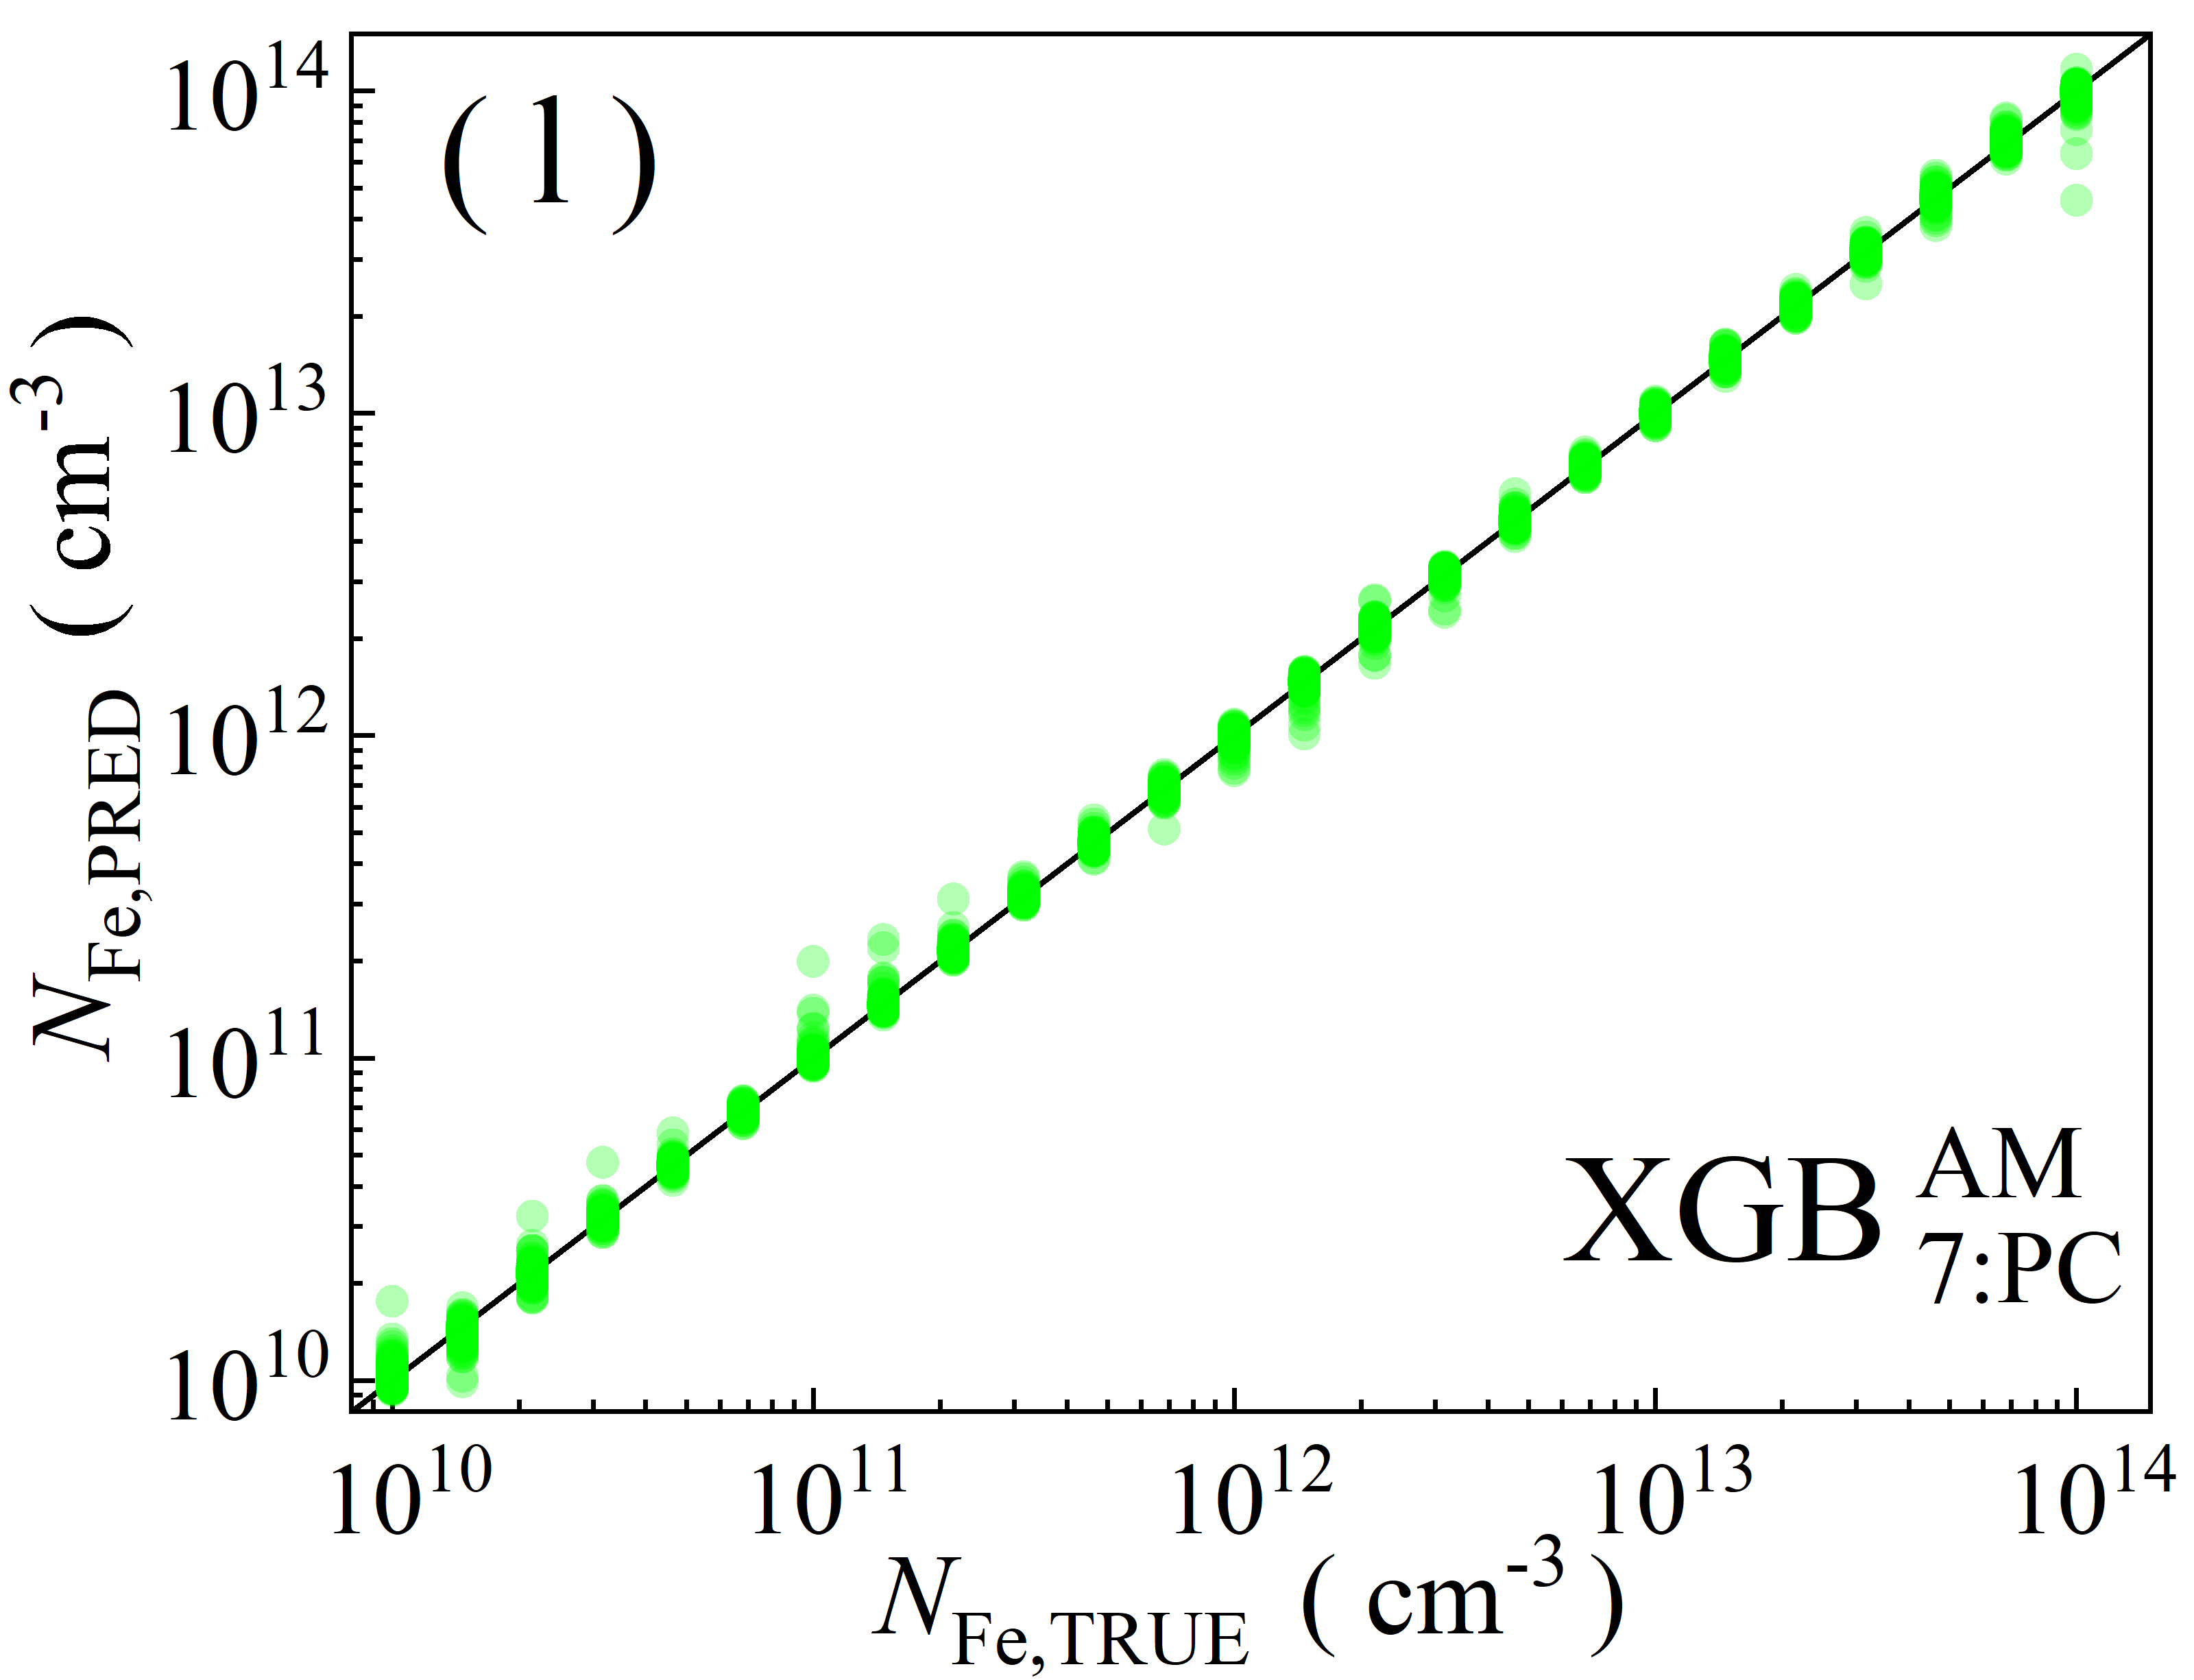
\includegraphics[width=0.24\linewidth]{Fig3l.png}
     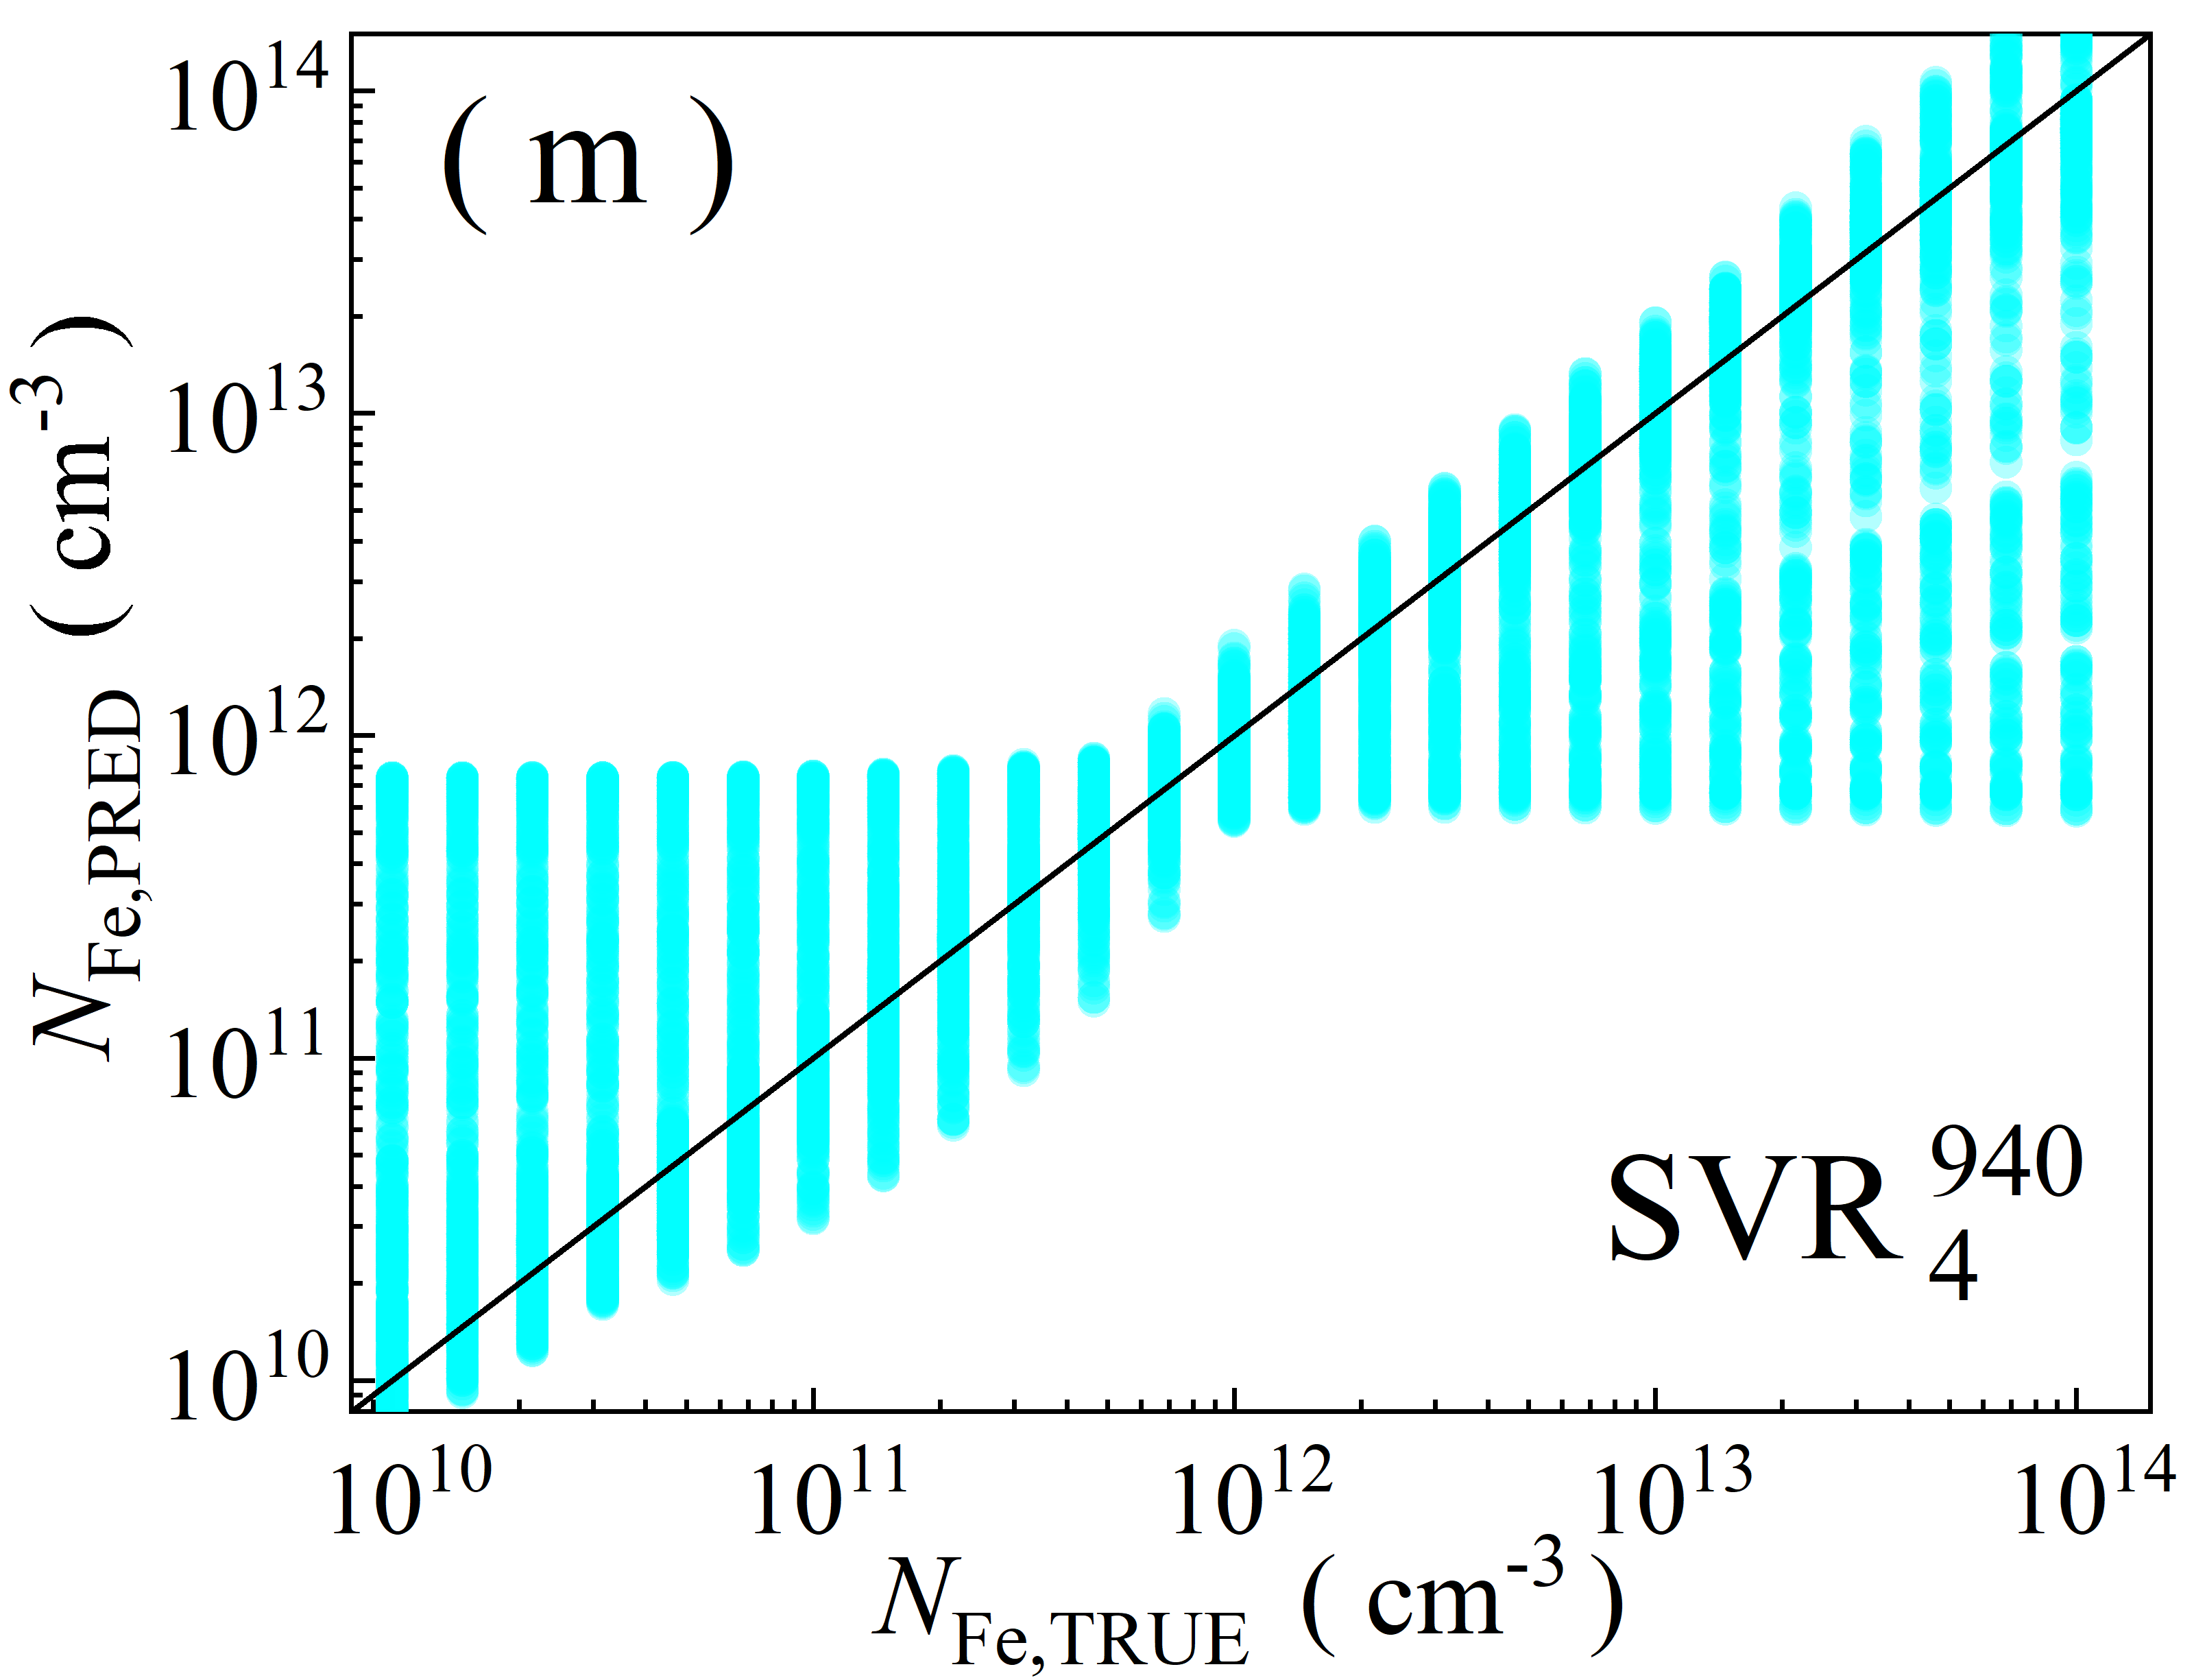
\includegraphics[width=0.24\linewidth]{Fig3m.png}
     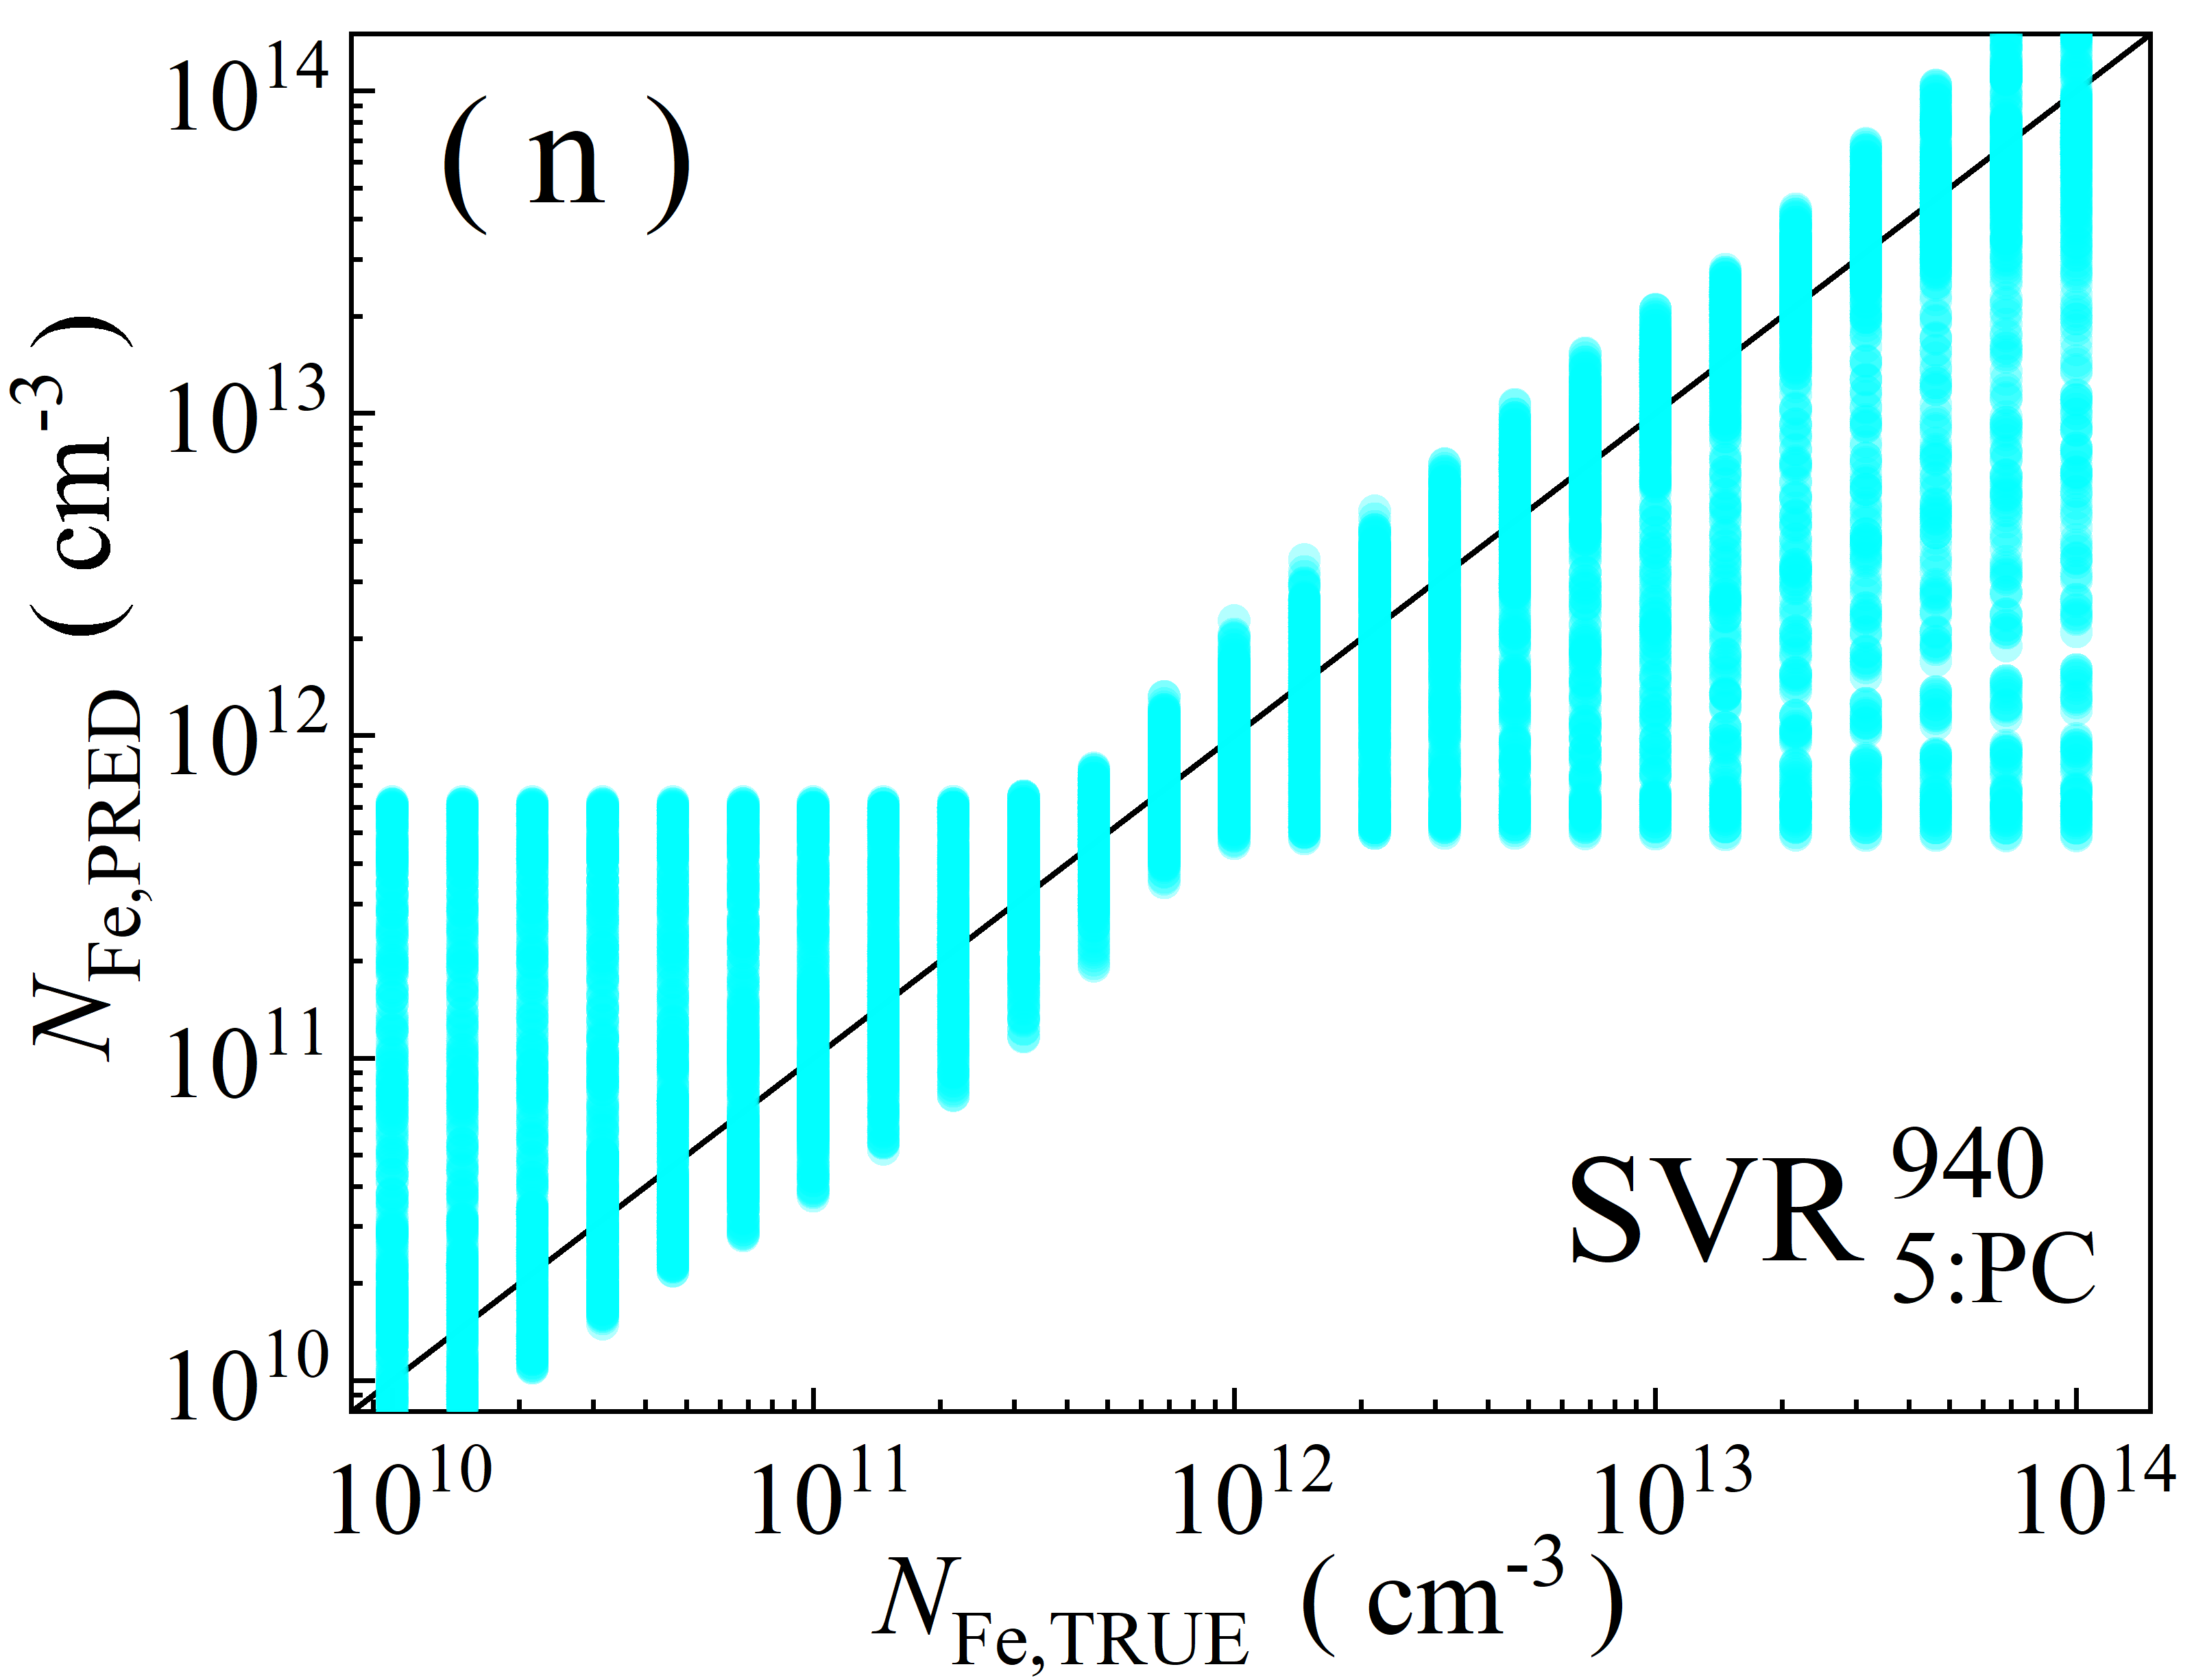
\includegraphics[width=0.24\linewidth]{Fig3n.png}
     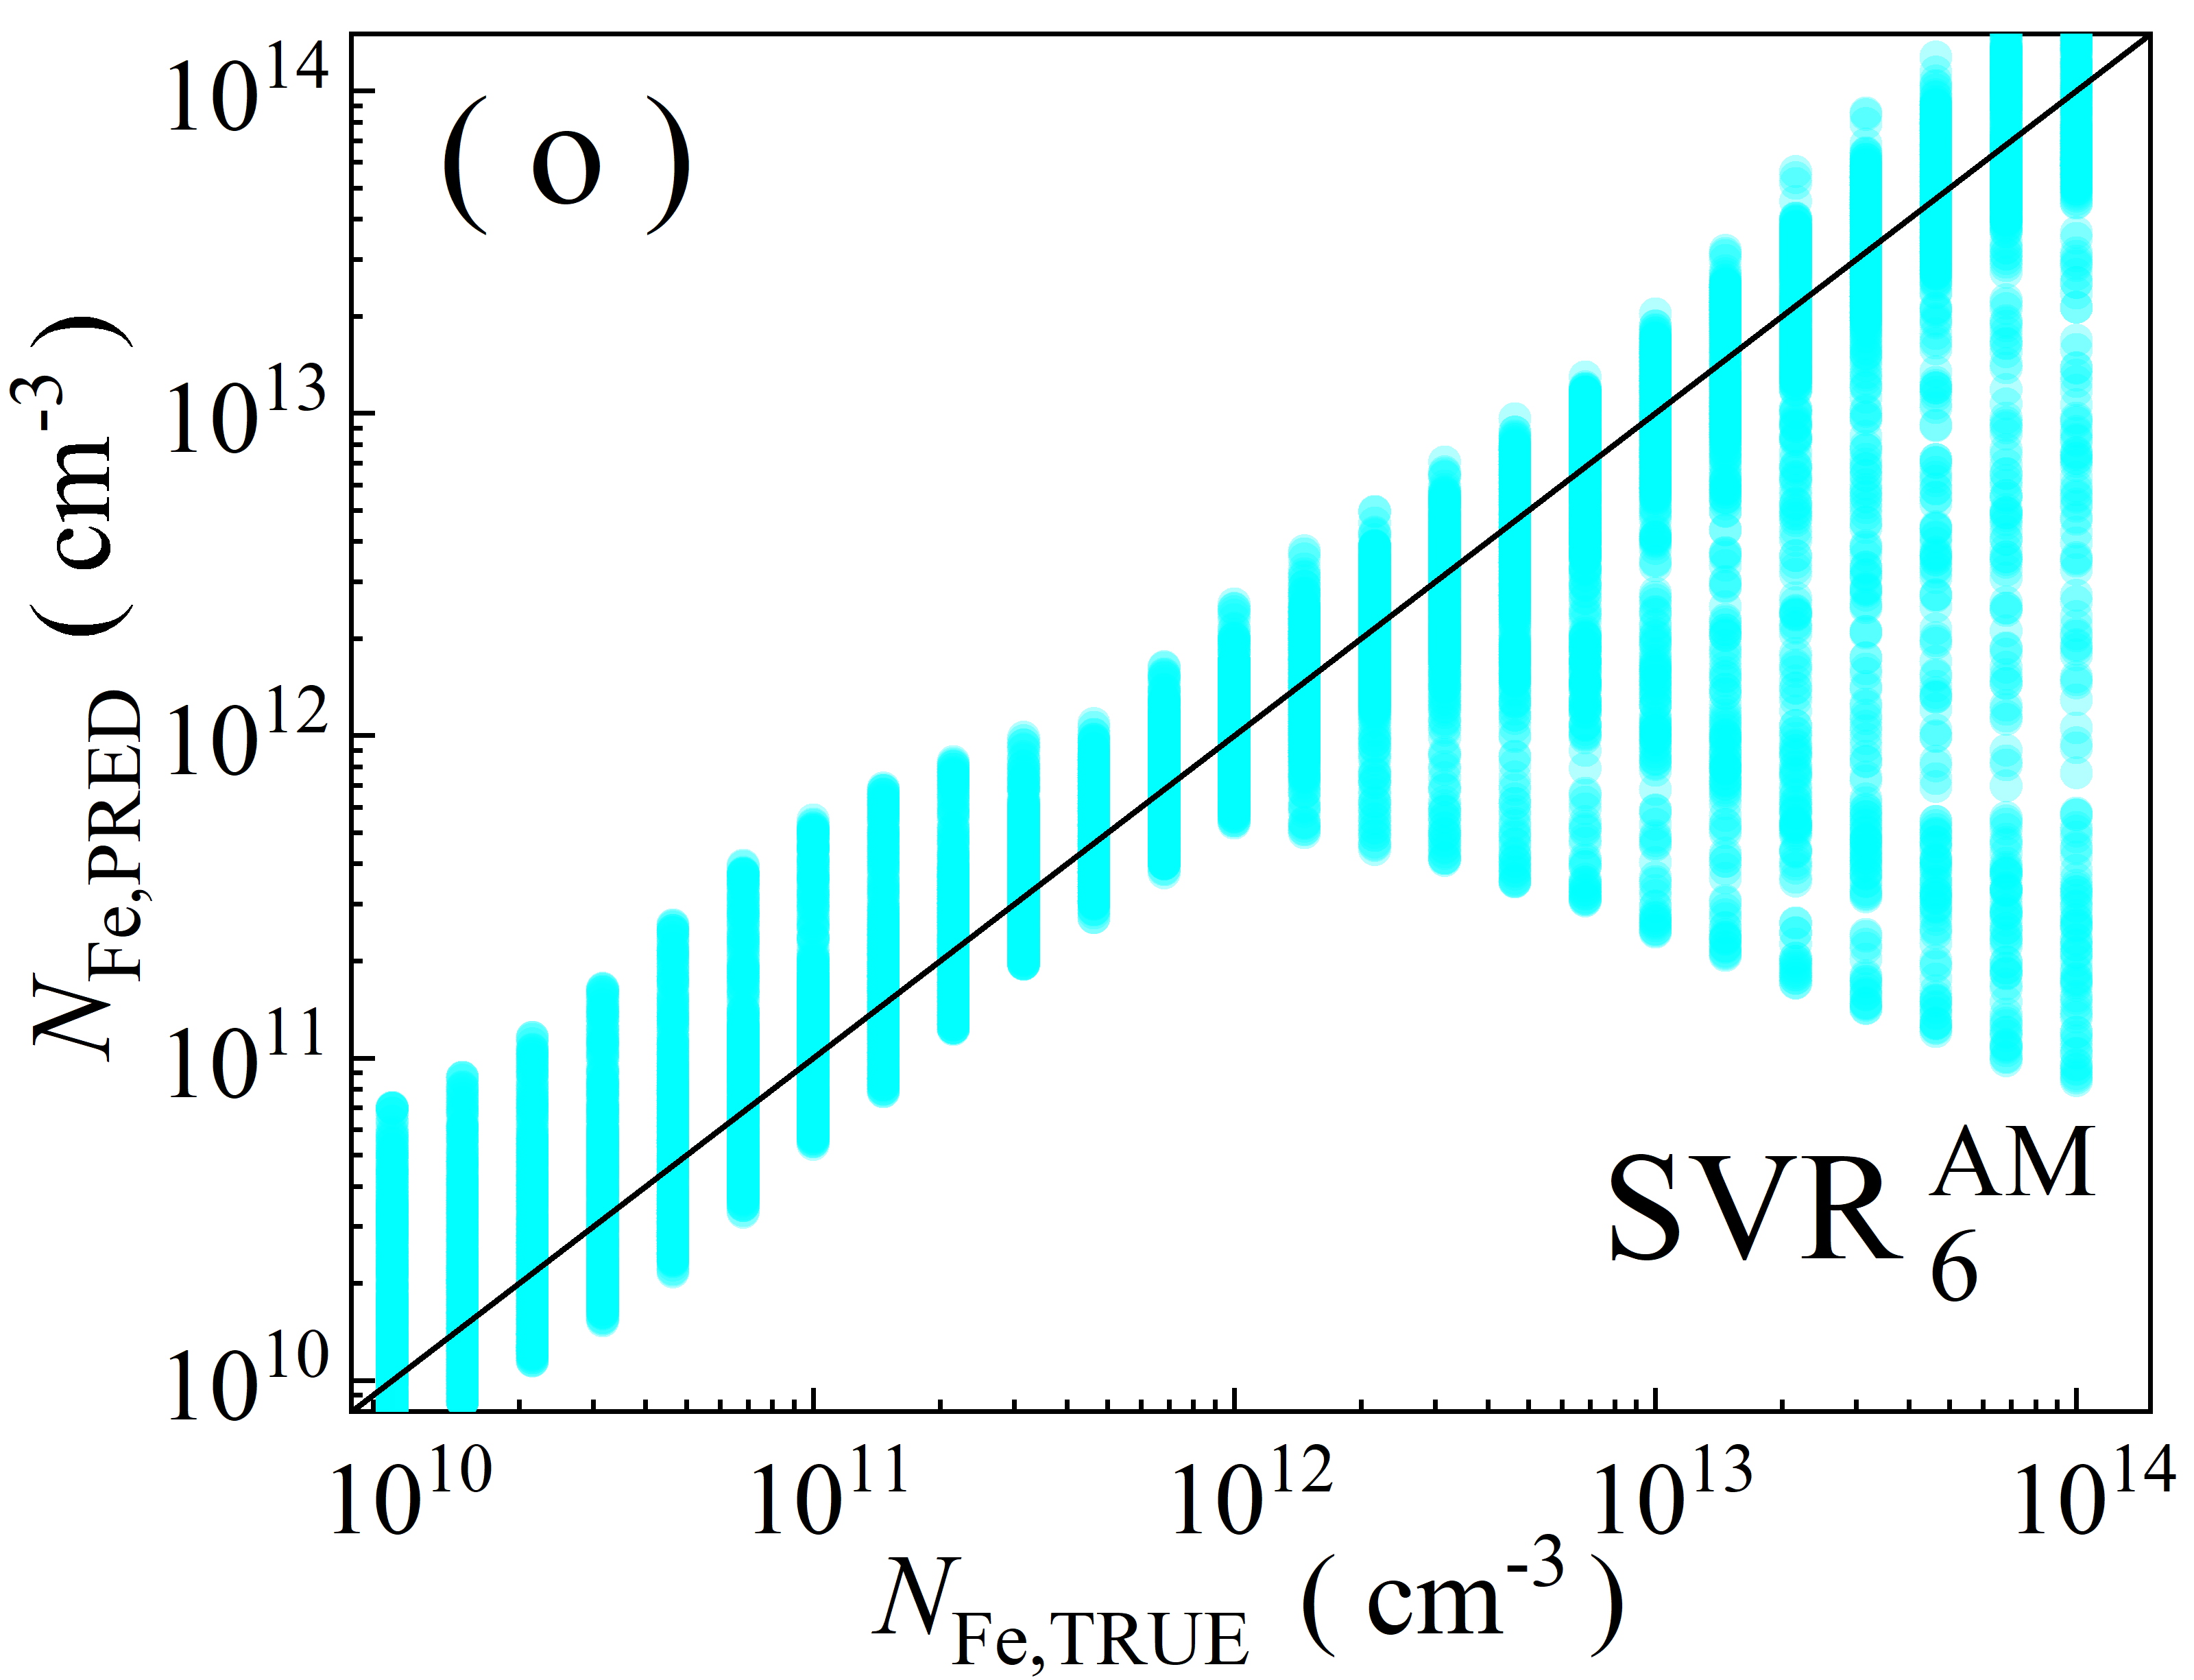
\includegraphics[width=0.24\linewidth]{Fig3o.png}
     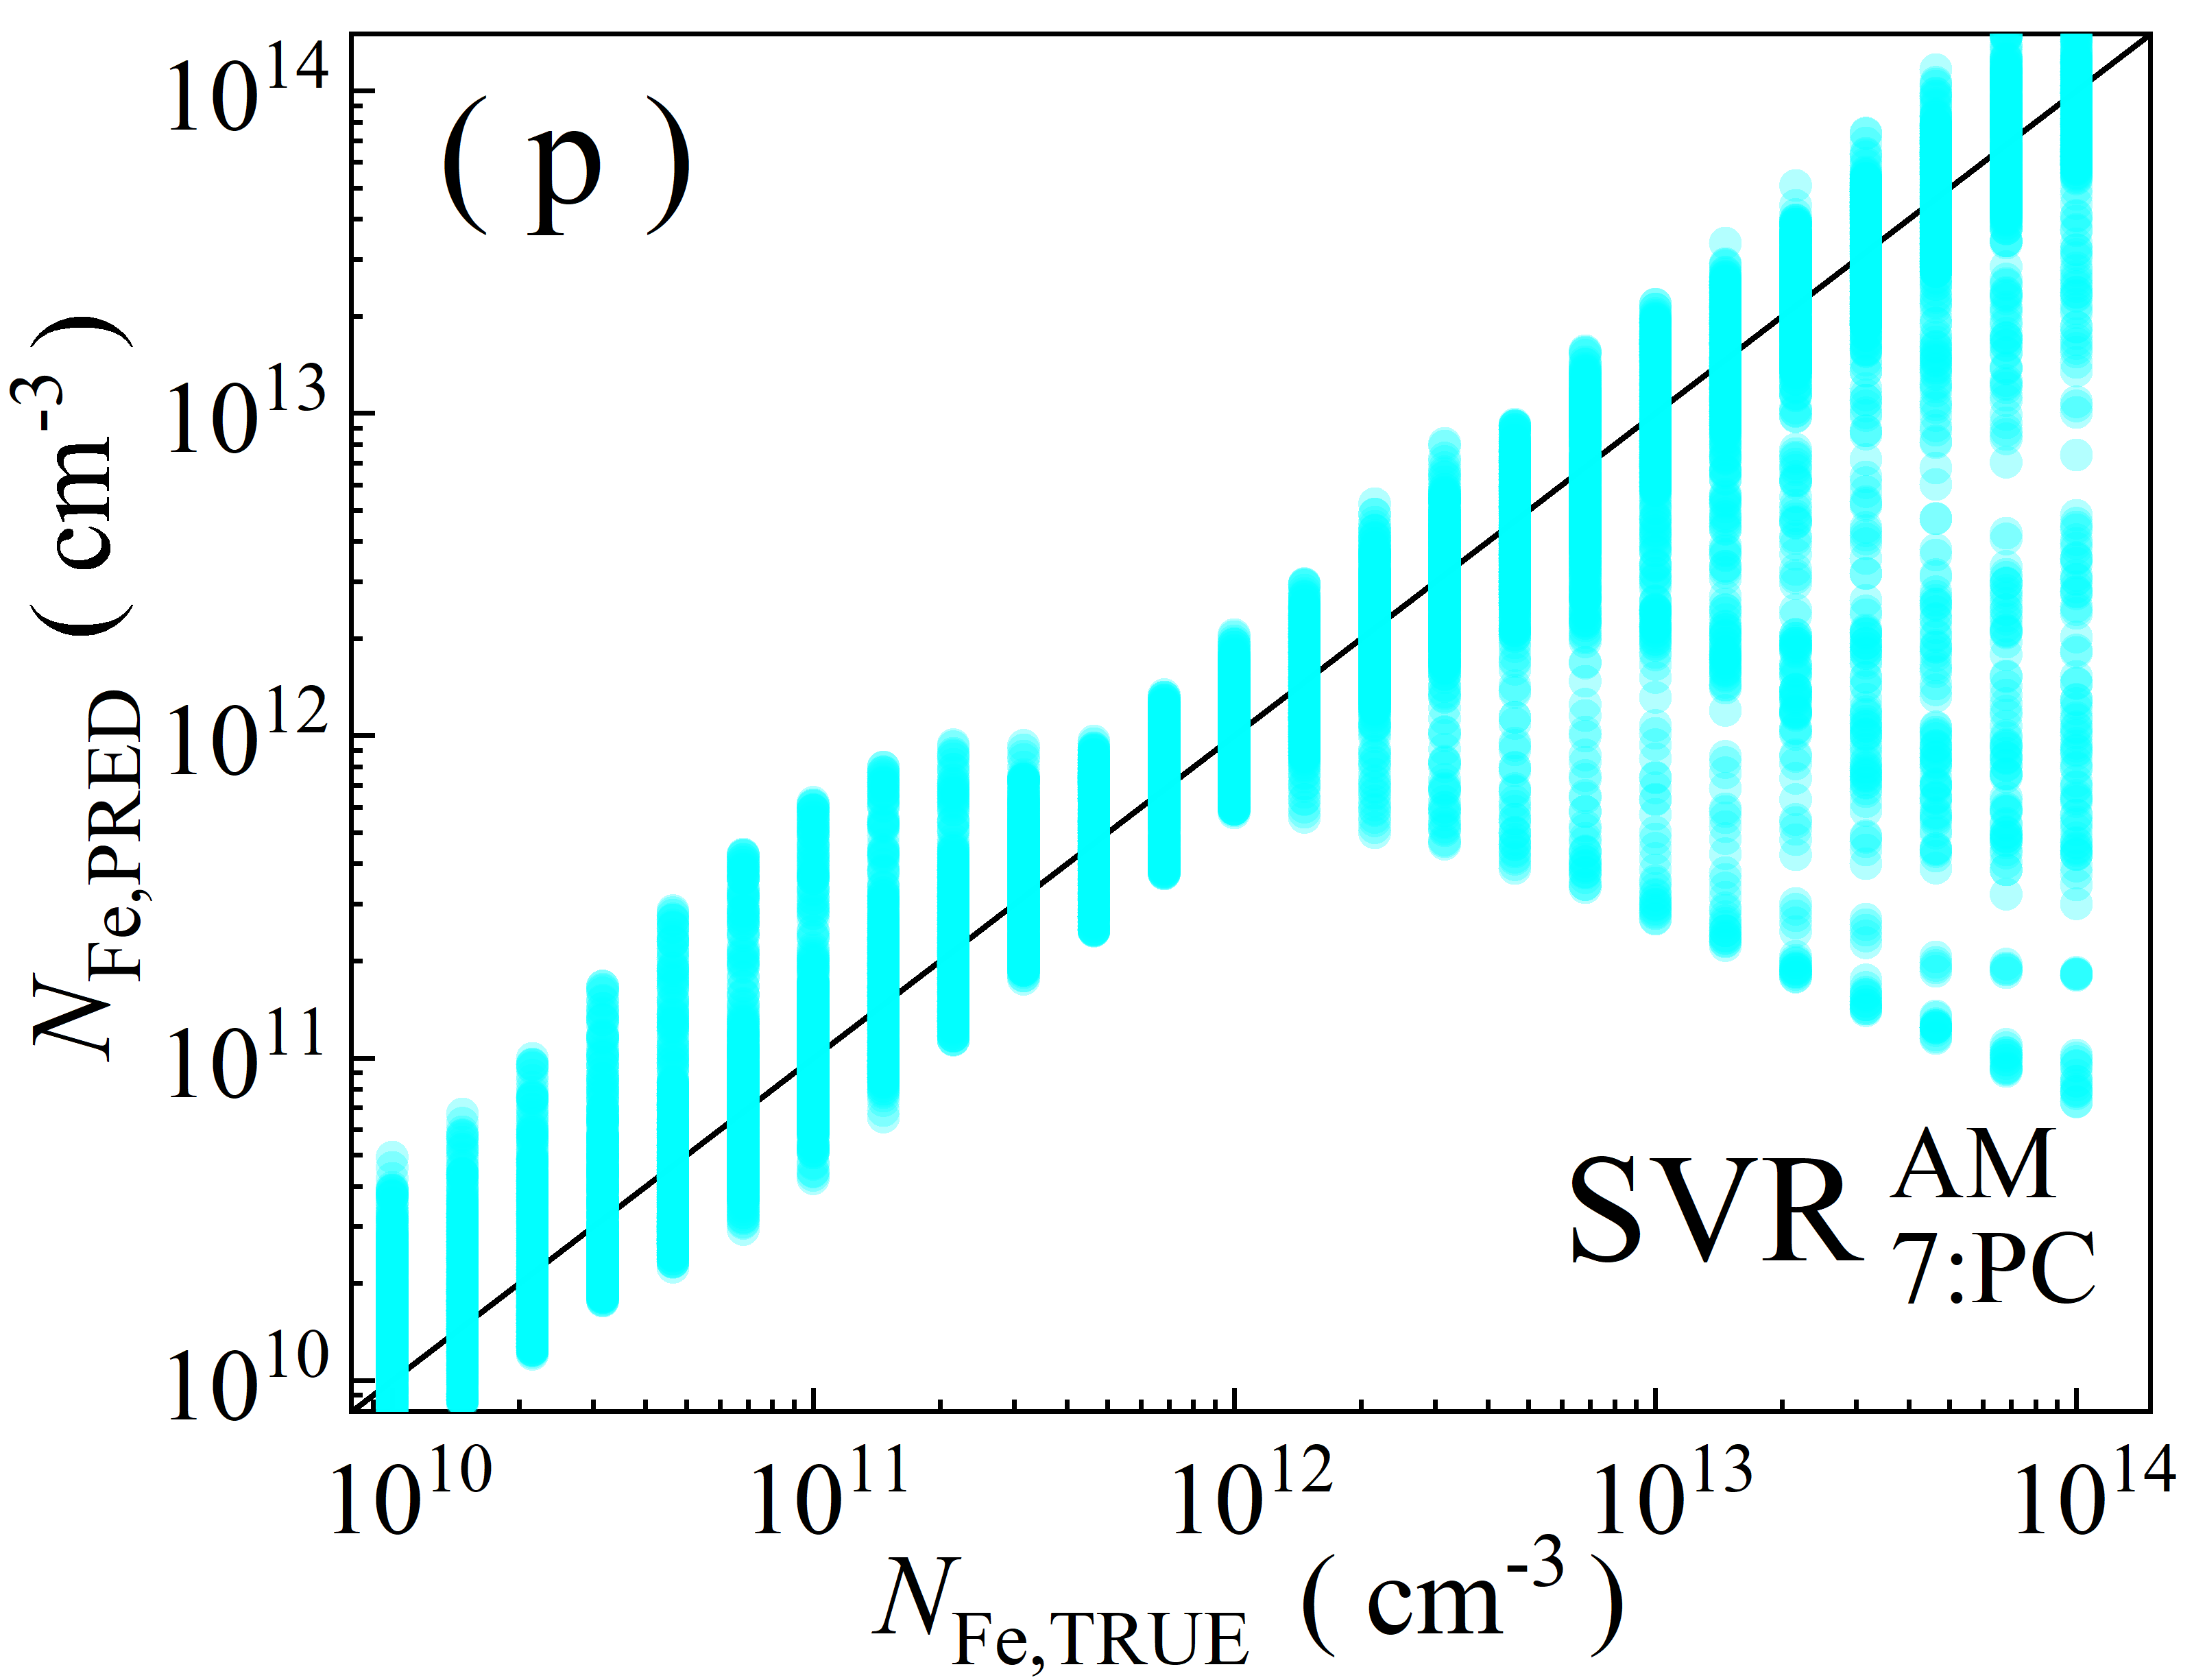
\includegraphics[width=0.24\linewidth]{Fig3p.png}
     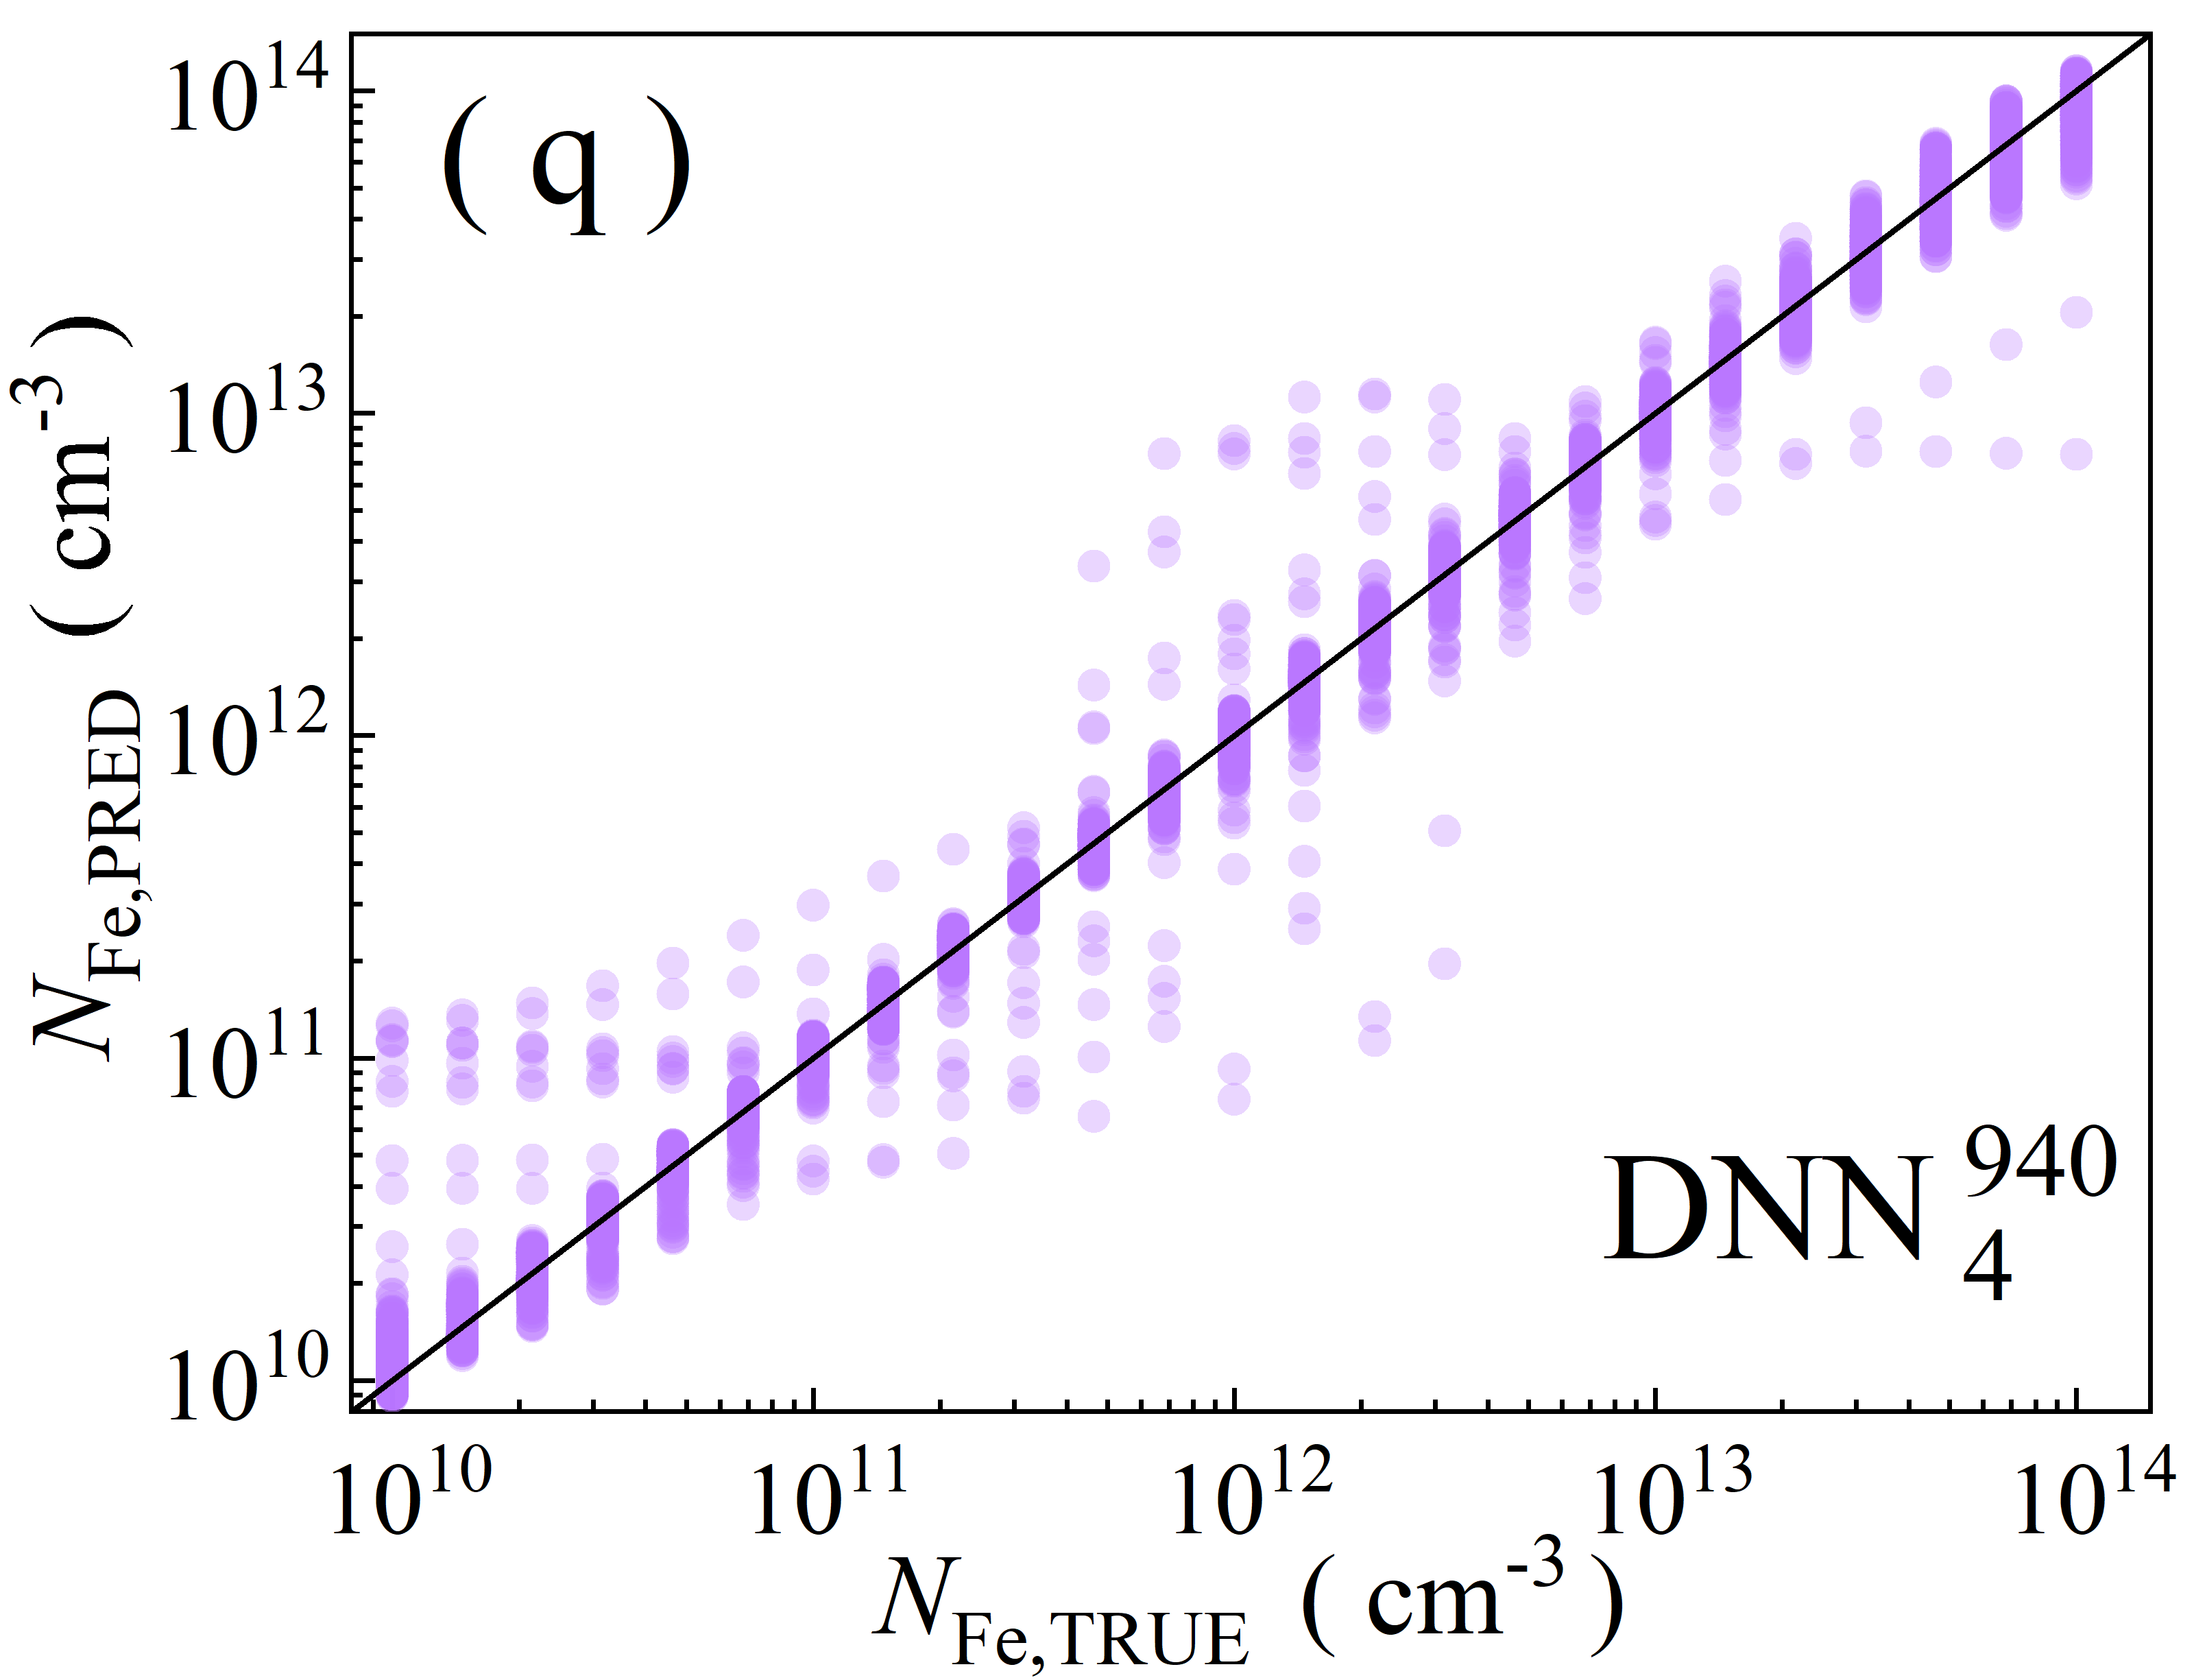
\includegraphics[width=0.24\linewidth]{Fig3q.png}
     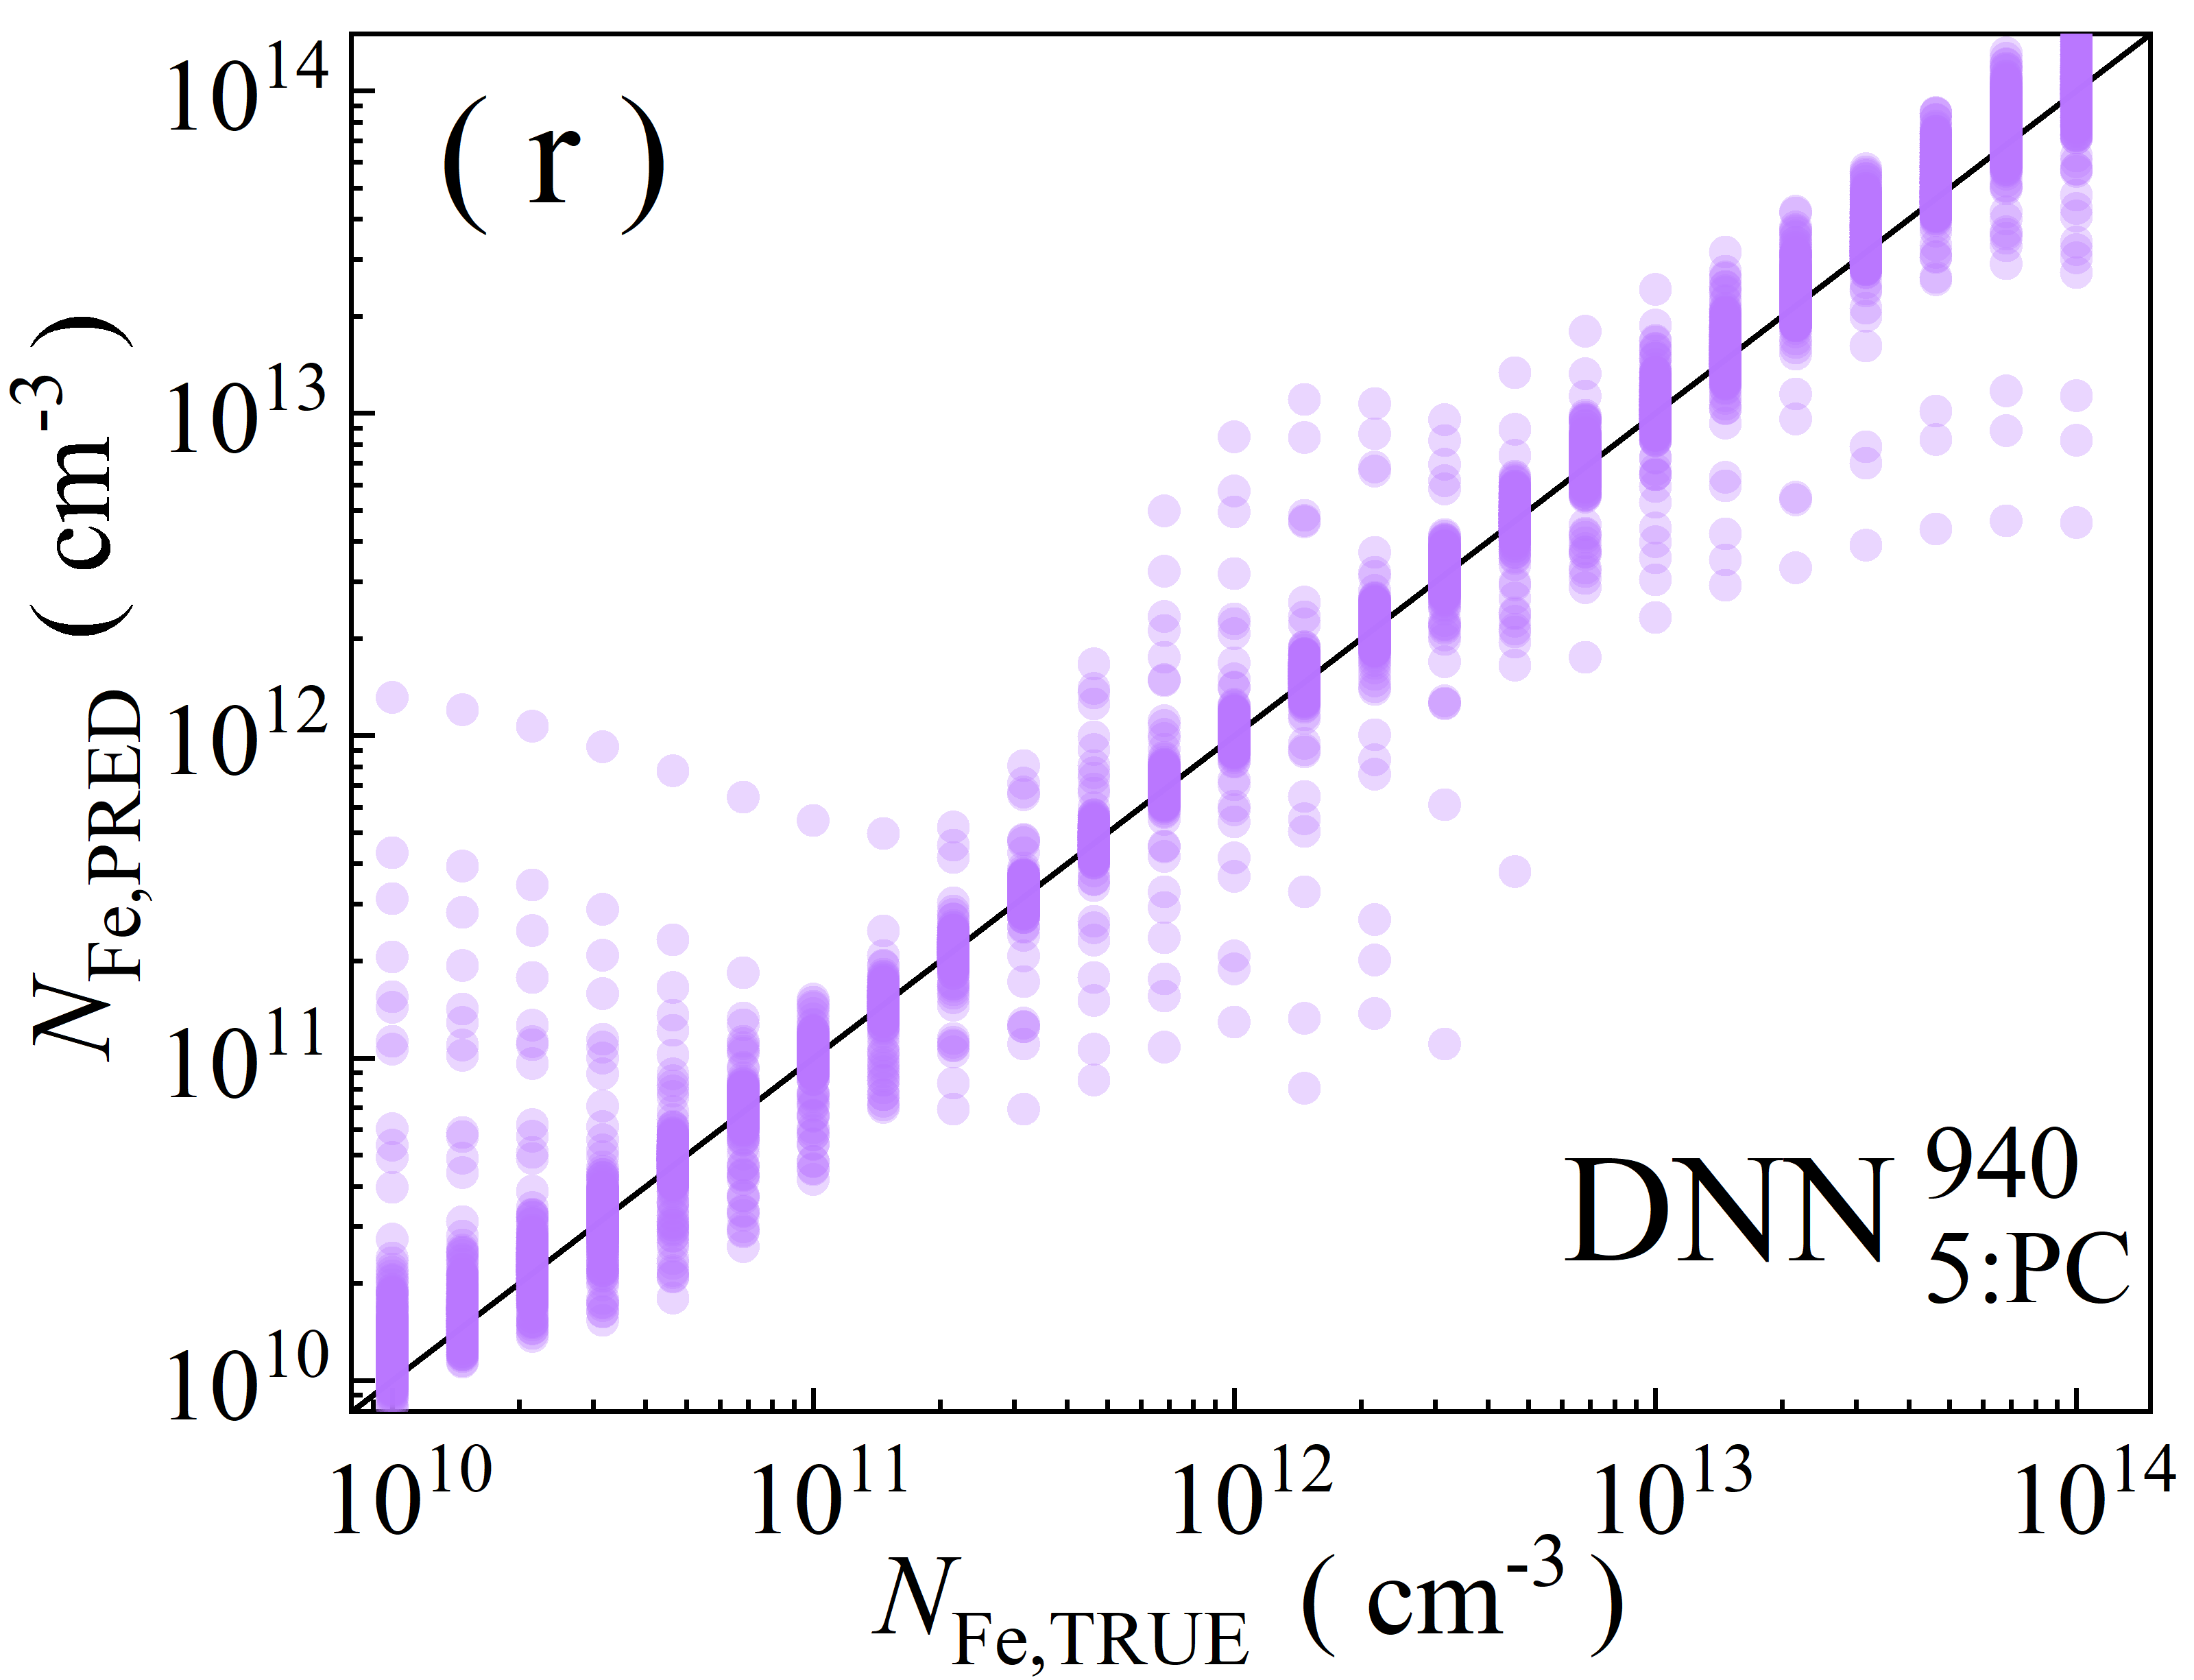
\includegraphics[width=0.24\linewidth]{Fig3r.png}
     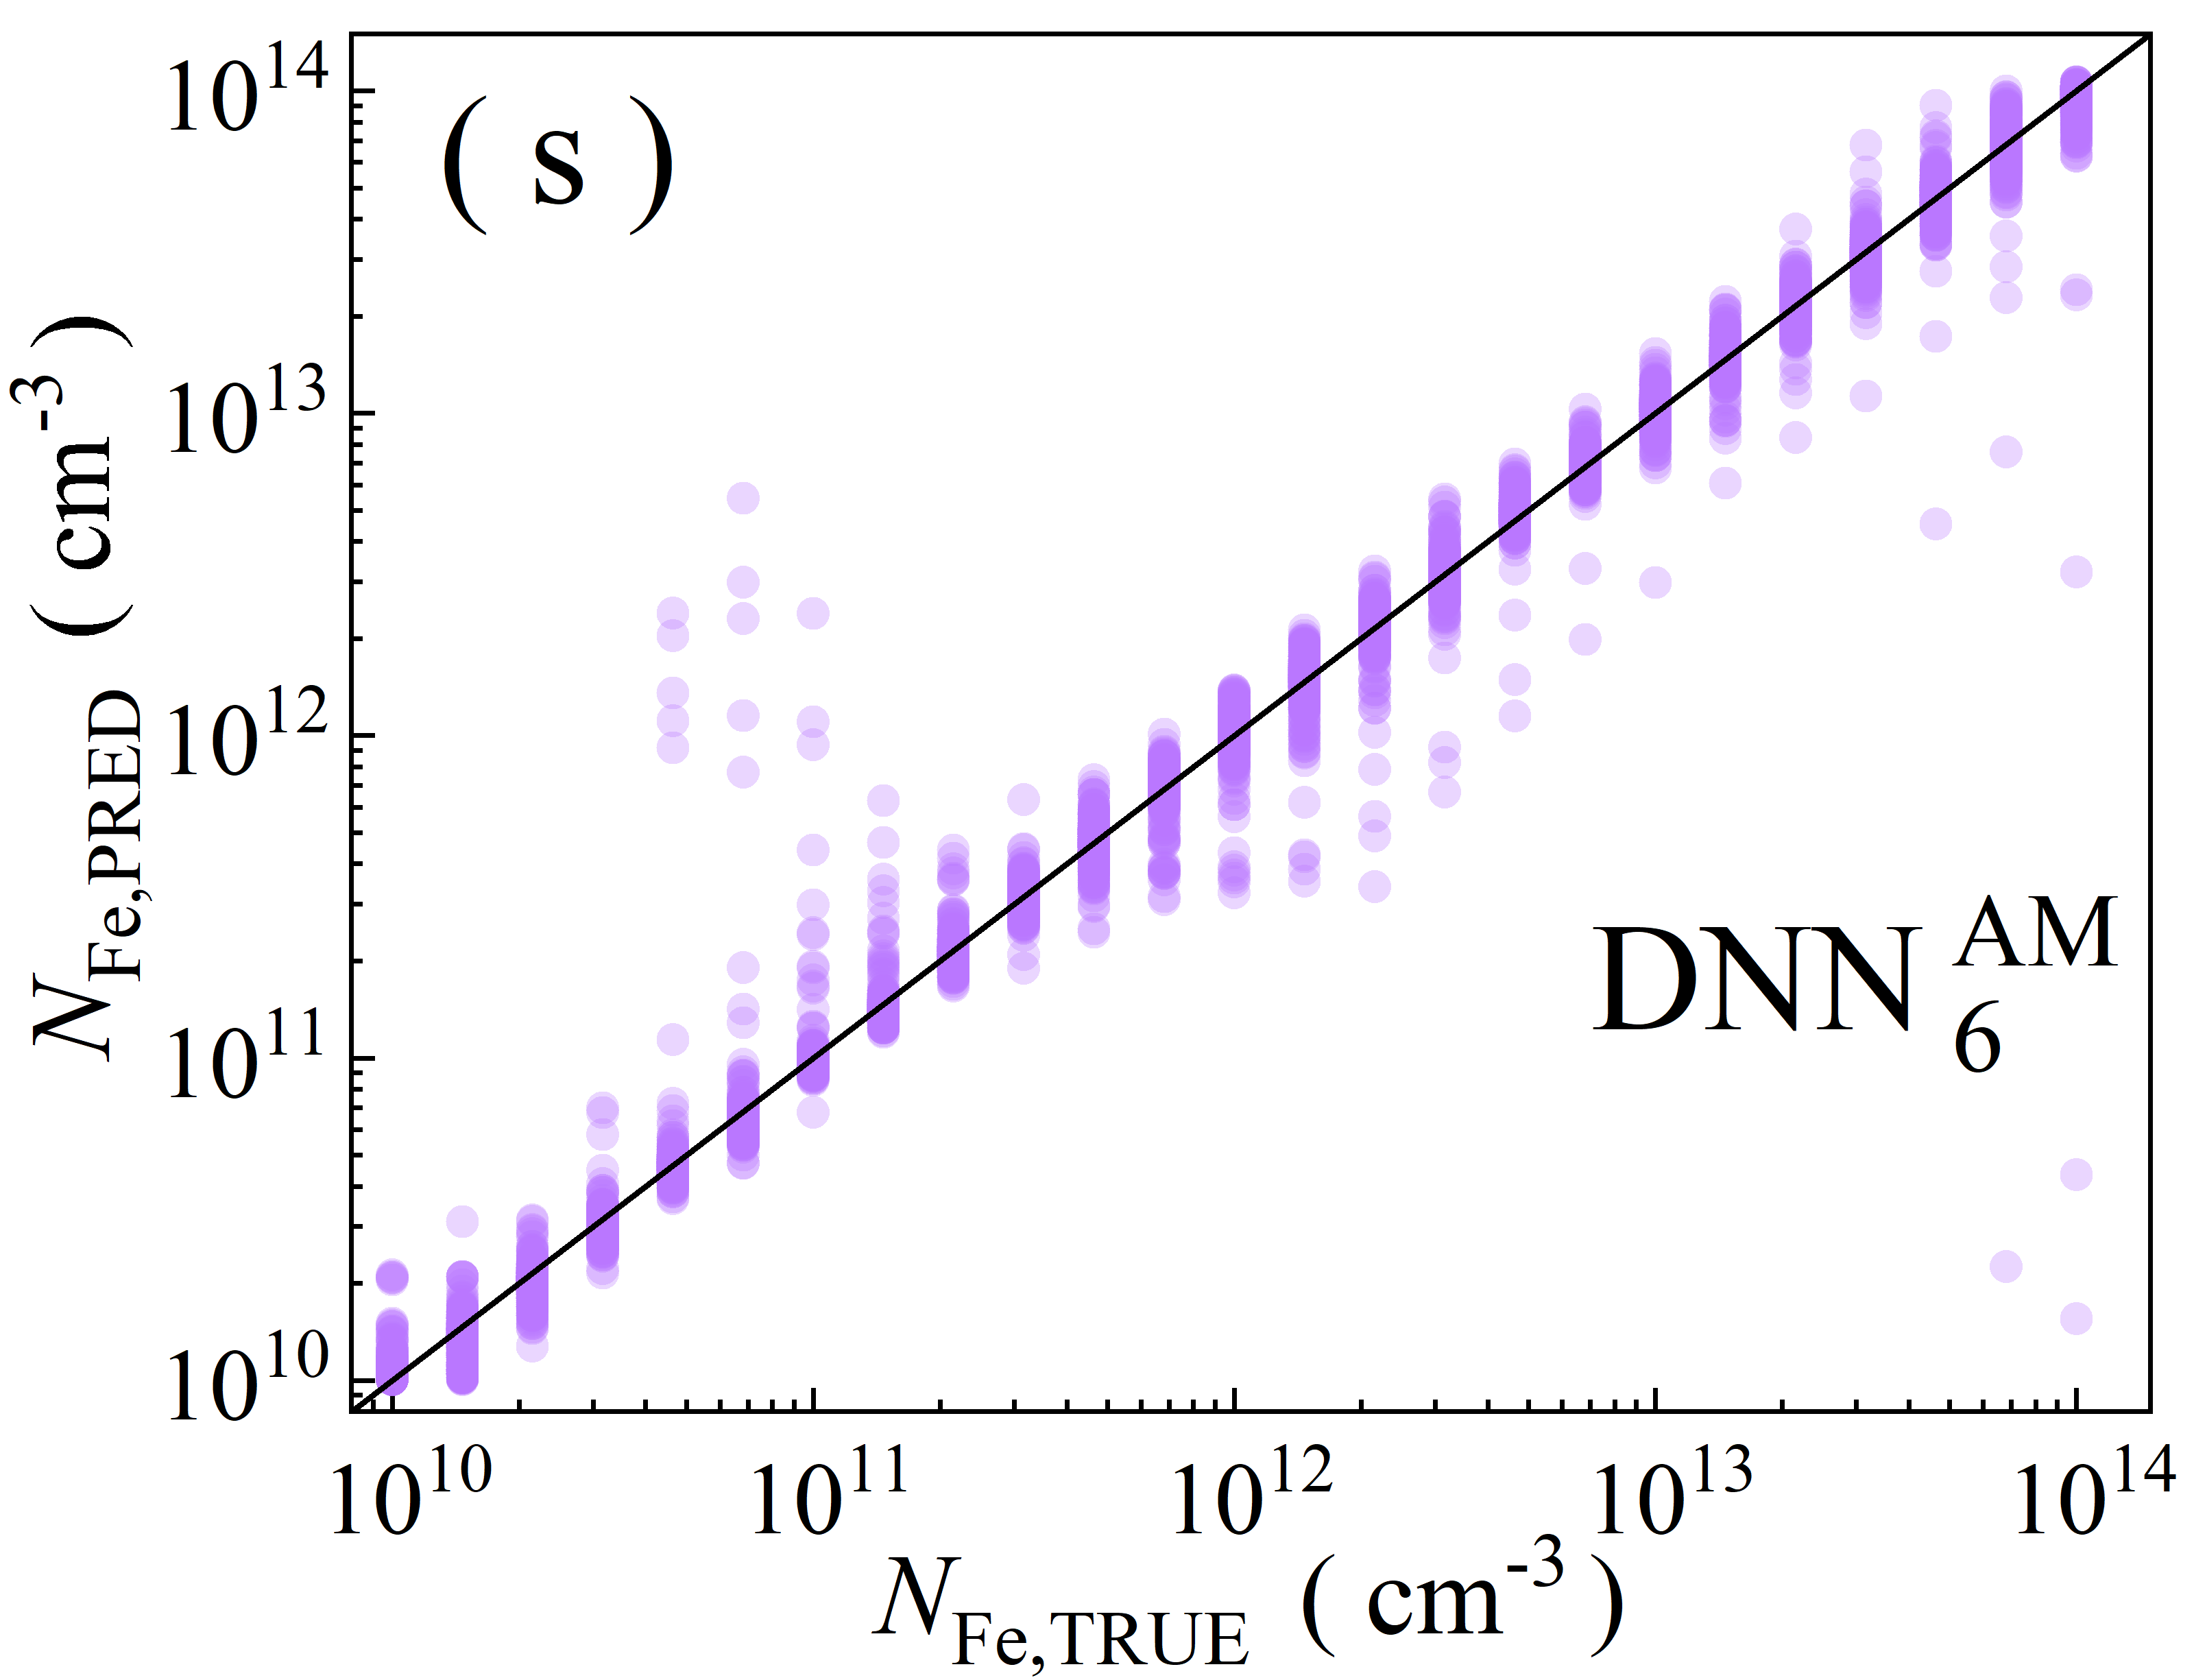
\includegraphics[width=0.24\linewidth]{Fig3s.png}
     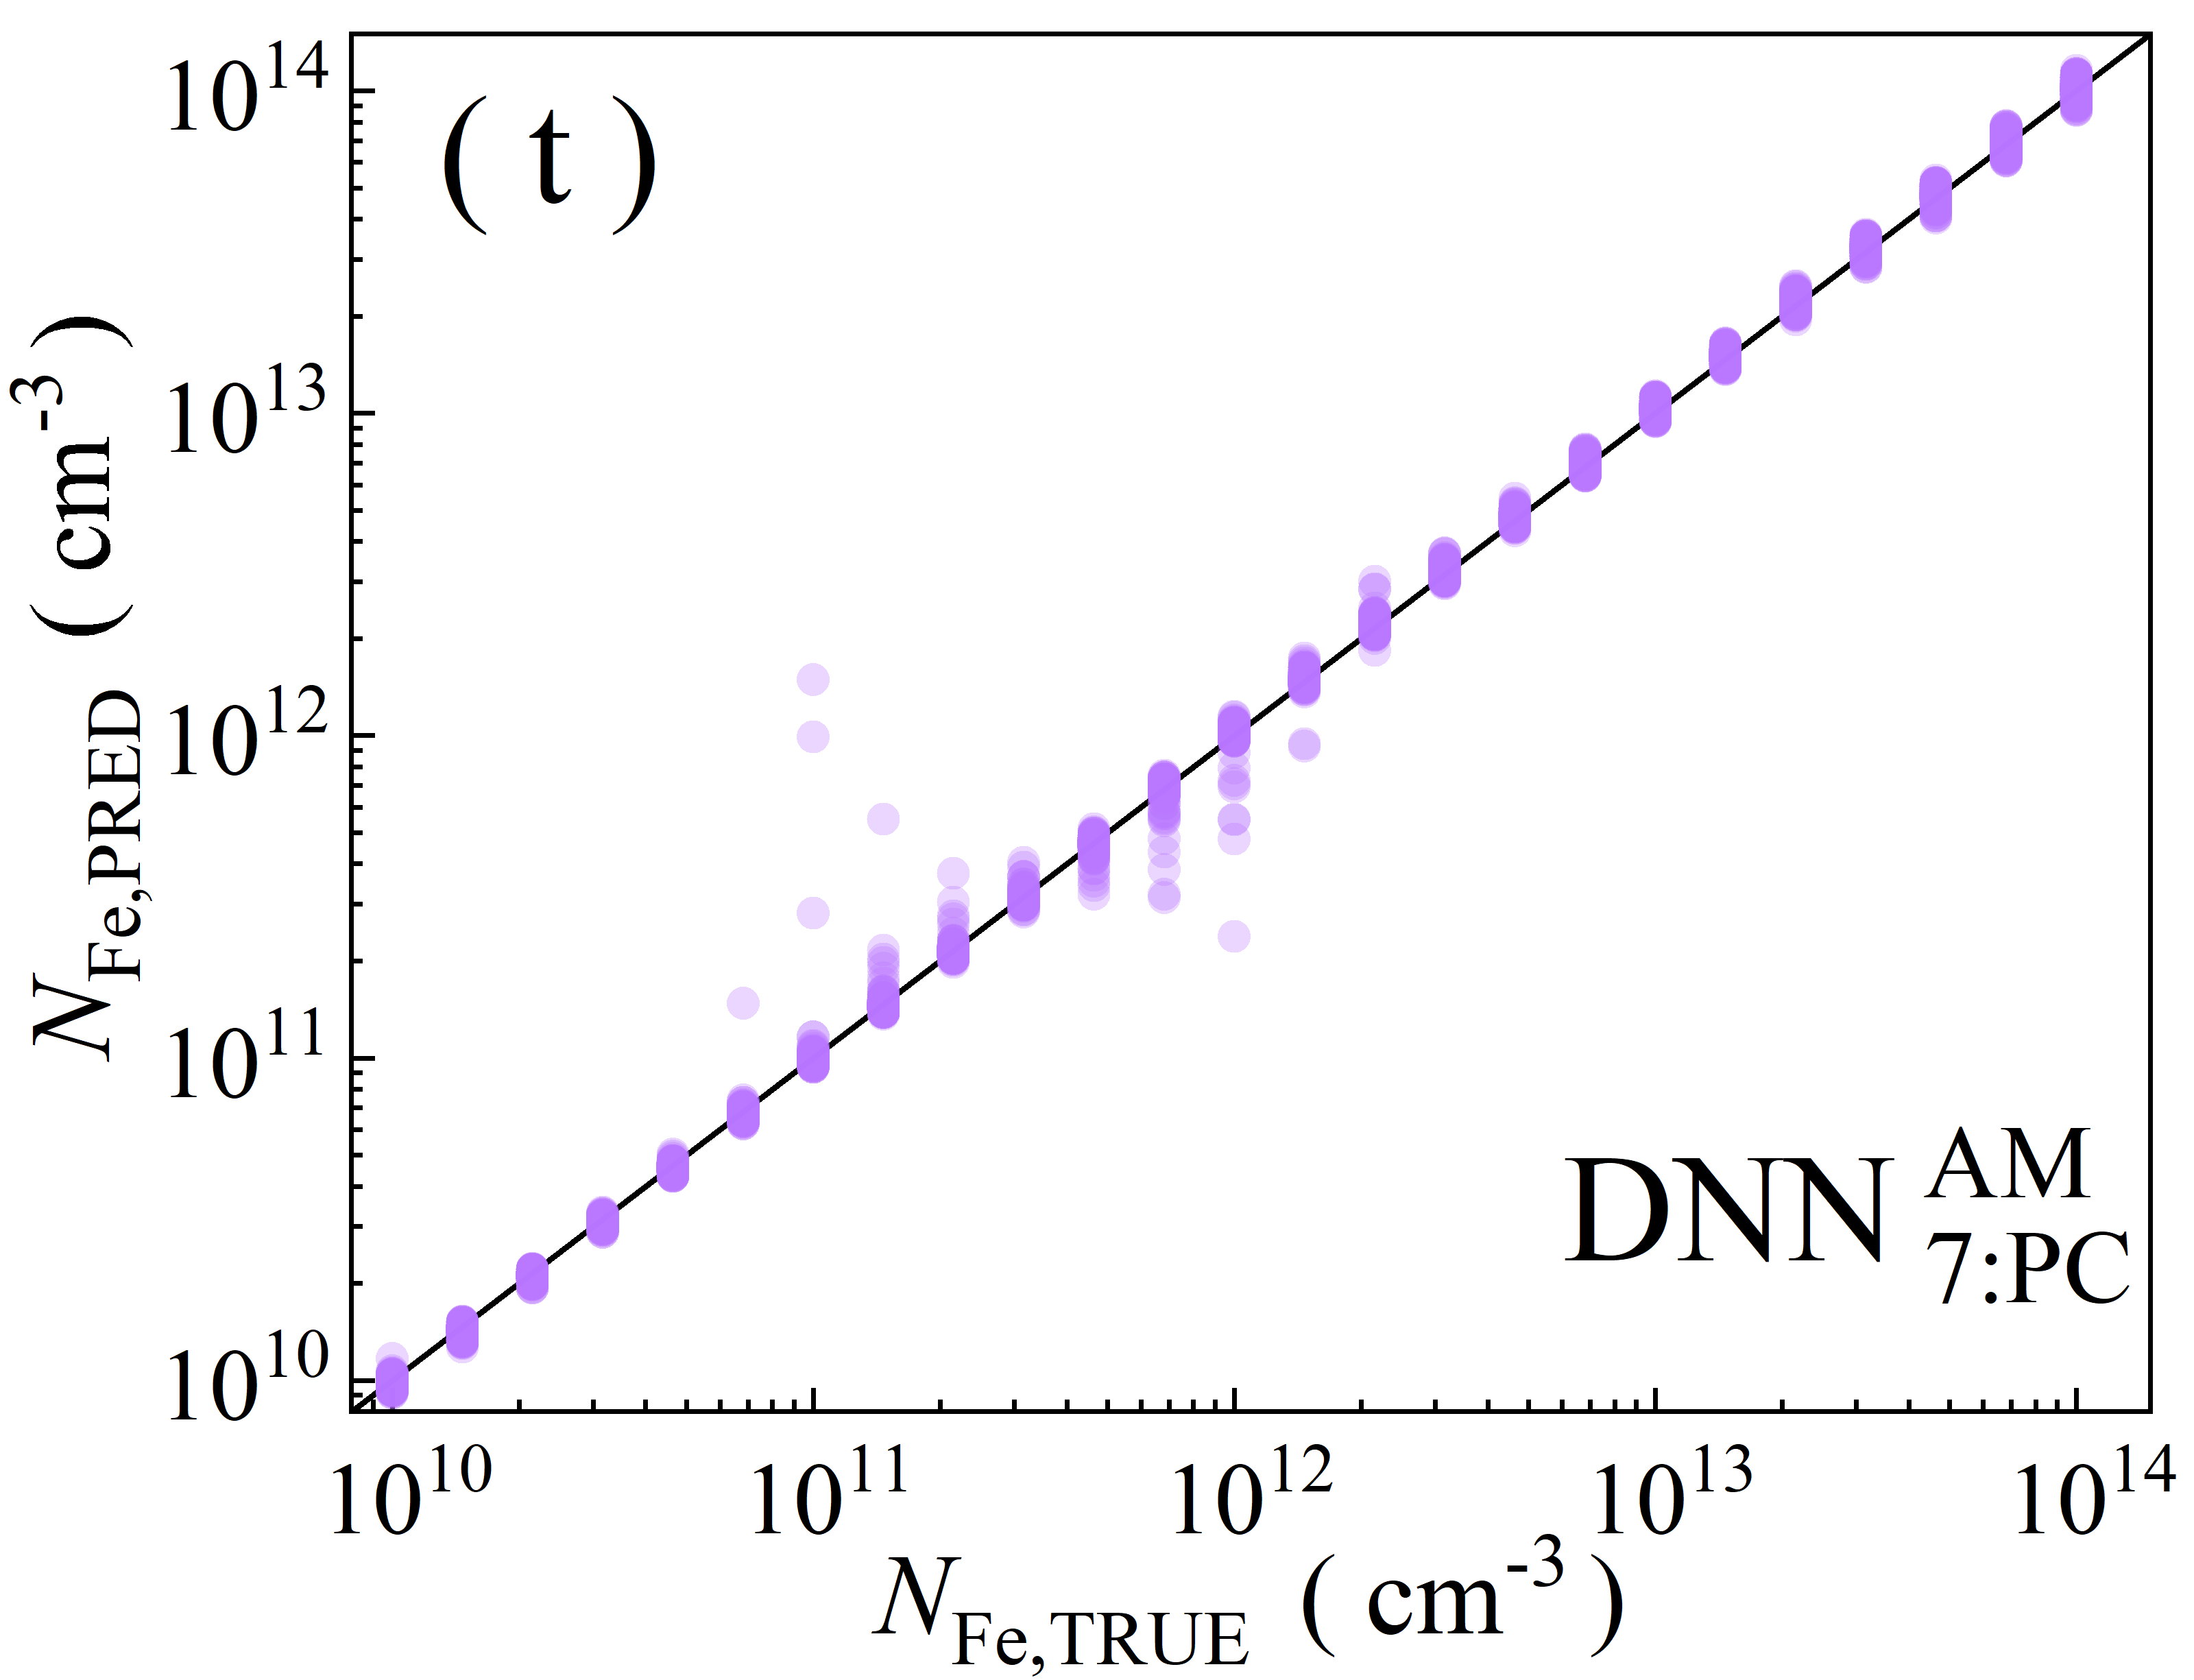
\includegraphics[width=0.24\linewidth]{Fig3t.png}
	  \caption{Scatter plots compare reference iron concentrations with ML--predicted values during the training phase.
The ML algorithms include RF (a--d), GB (e--h), XGB (i--l), SVR (m--p), and DNN (q--t).
The data come from simulation under monochromatic (a, b, e, f, i, j, m, n, q, r) and AM1.5 illumination (c, d, g, h, k, l, o, p, s, t).
 Panels b, d, f, h, j, l, n, p, r, and t include PCA. The input feature dimensions are 4 (a, e, i, m, q), 5 (b, f, j, n, r), 6 (c, g, k, o, s), and 7 (d, h, l, p, t).
 The black lines are the identified lines serving as the references.
}\label{fig3}
\end{figure}


As expected, increasing the number of descriptors enhances model performance (Fig.~\ref{fig4} and Fig.S7).
The only exception occurs under AM1.5 illumination with PCA, where adding a fifth descriptor may degrade predictions rather than improve them.
Overall, models trained on AM1.5 data exhibit significantly lower accuracy than those using monochromatic illumination, with errors approximately an order of magnitude higher.
Notably, models with four descriptors (or five with PCA) under AM1.5 appear unpromising, even for RF and GB.
Meanwhile, increasing the number of descriptors from six to seven offers little to no additional benefit in high--accuracy models
such as RF, GB, XGB, and, to some extent, DNN.


\begin{figure}
	\centering
     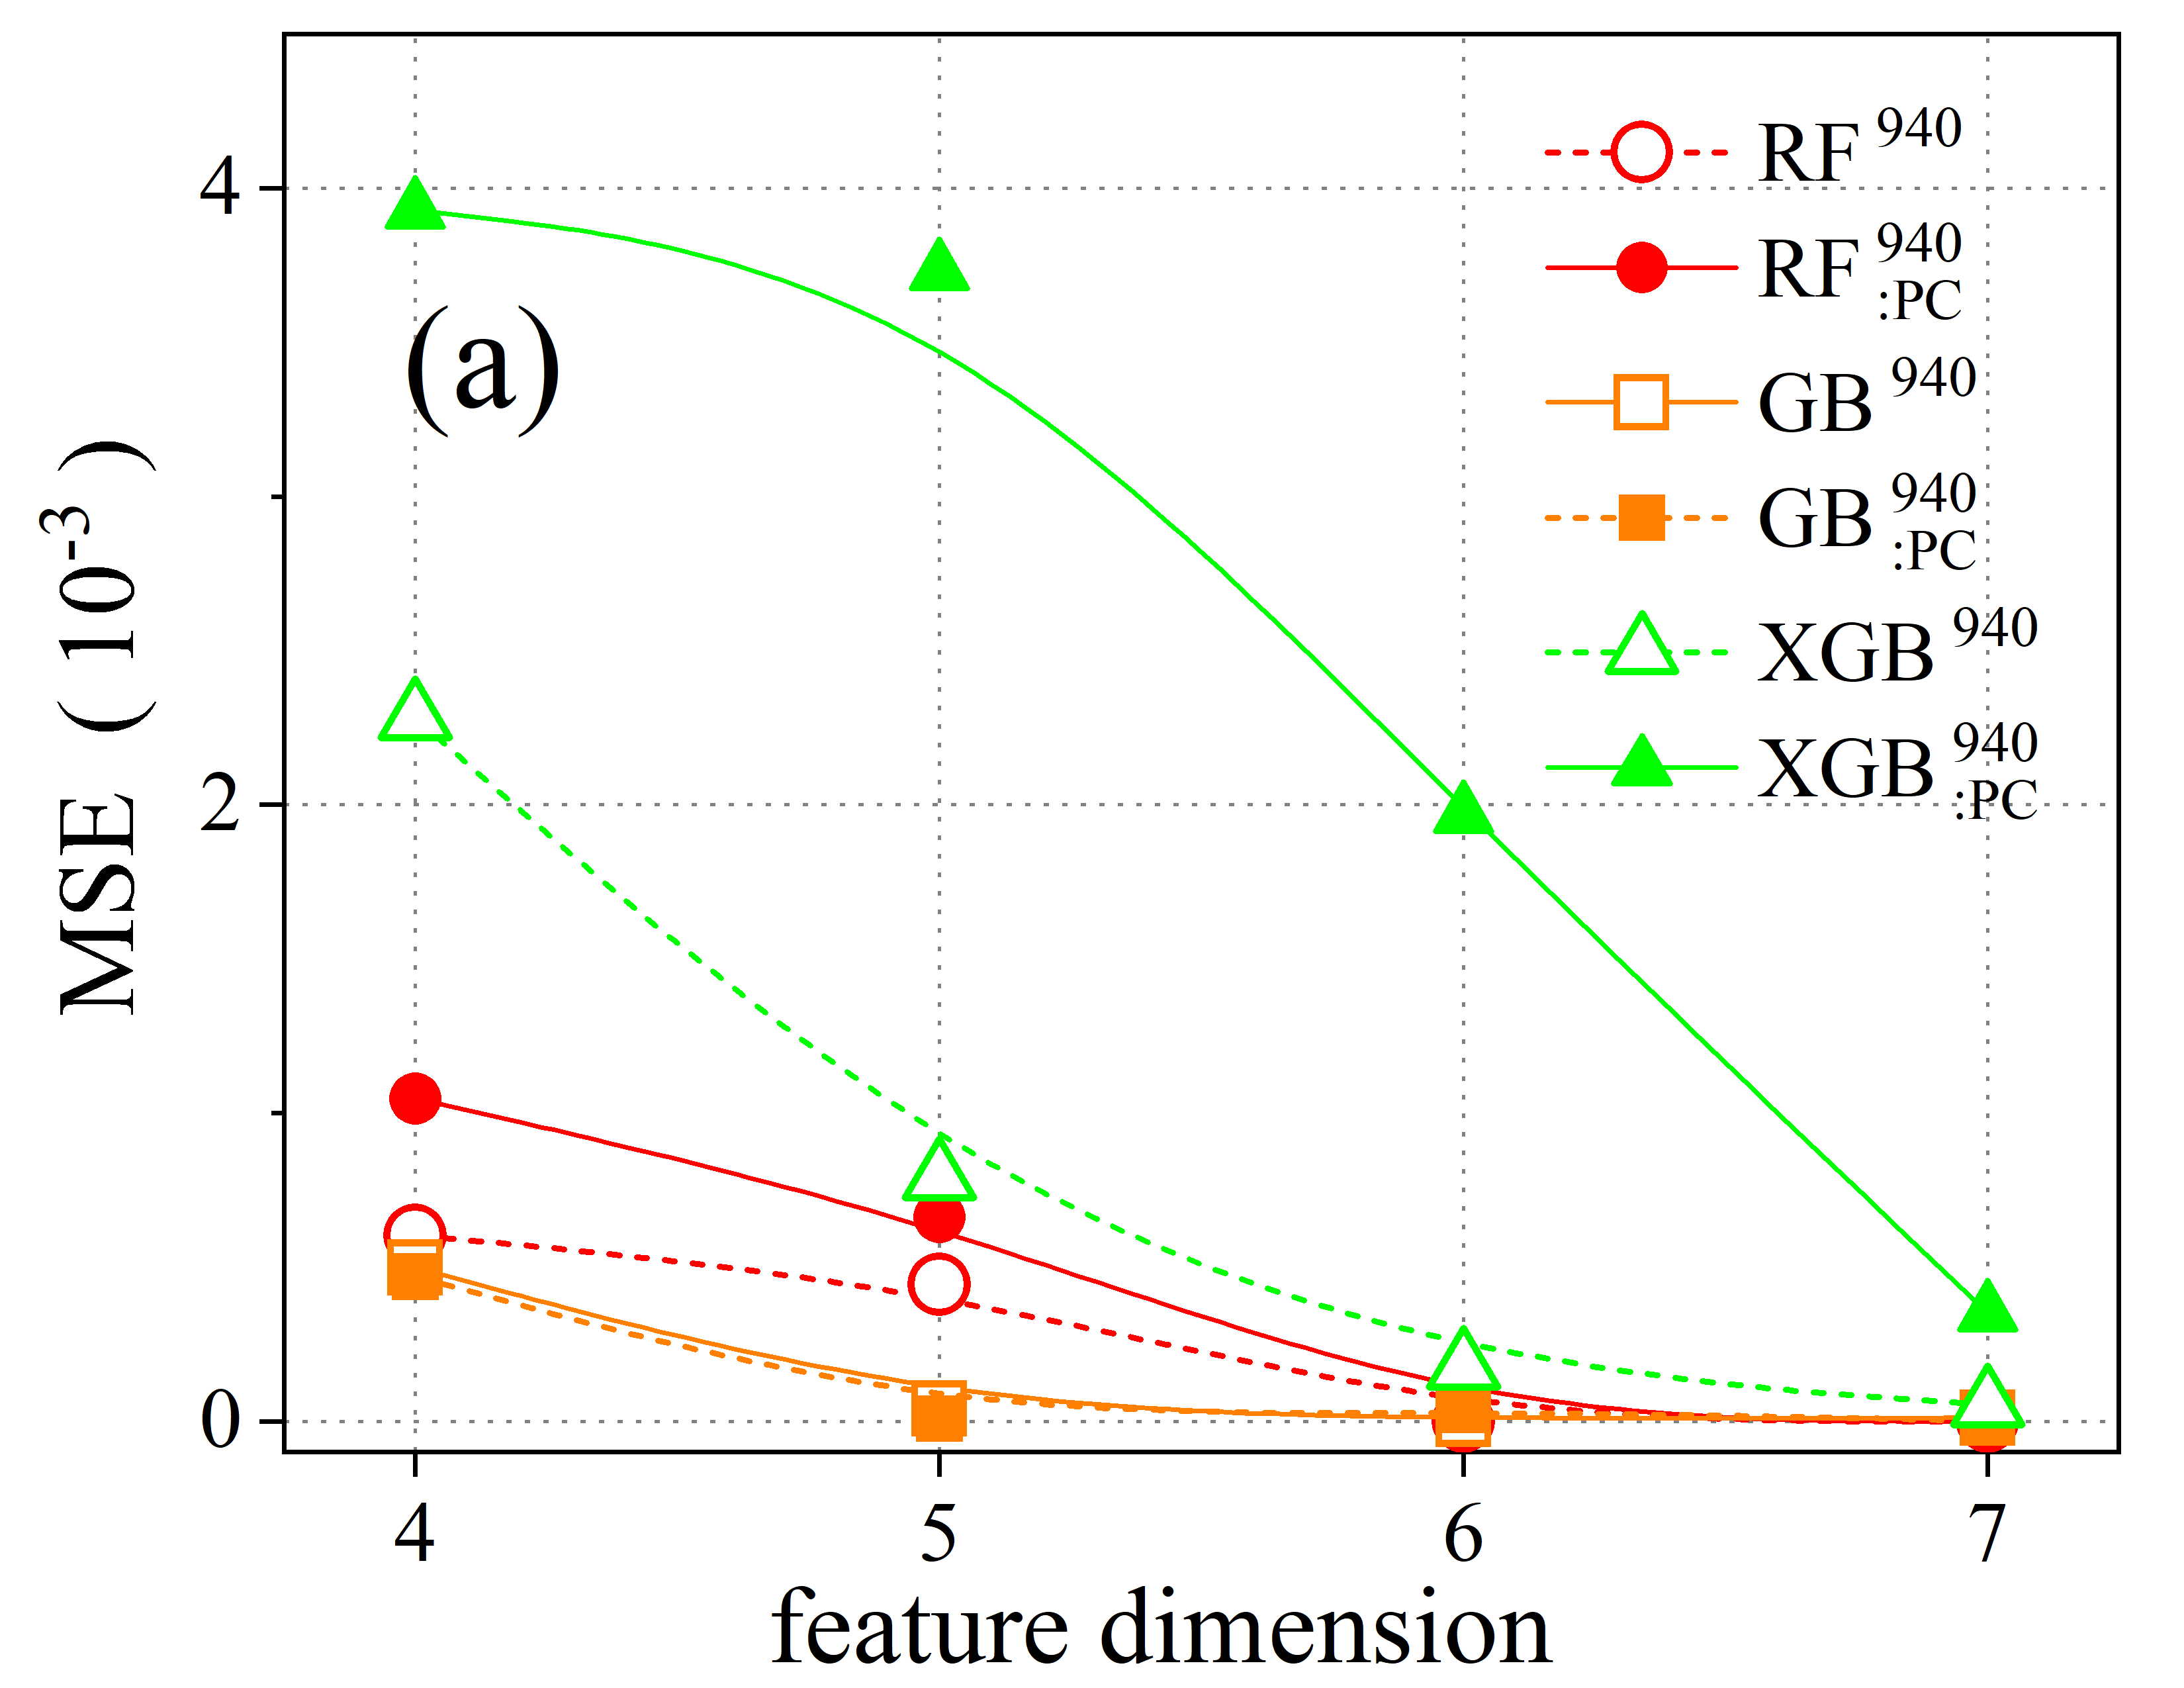
\includegraphics[width=0.4\linewidth]{Fig4a.png}
     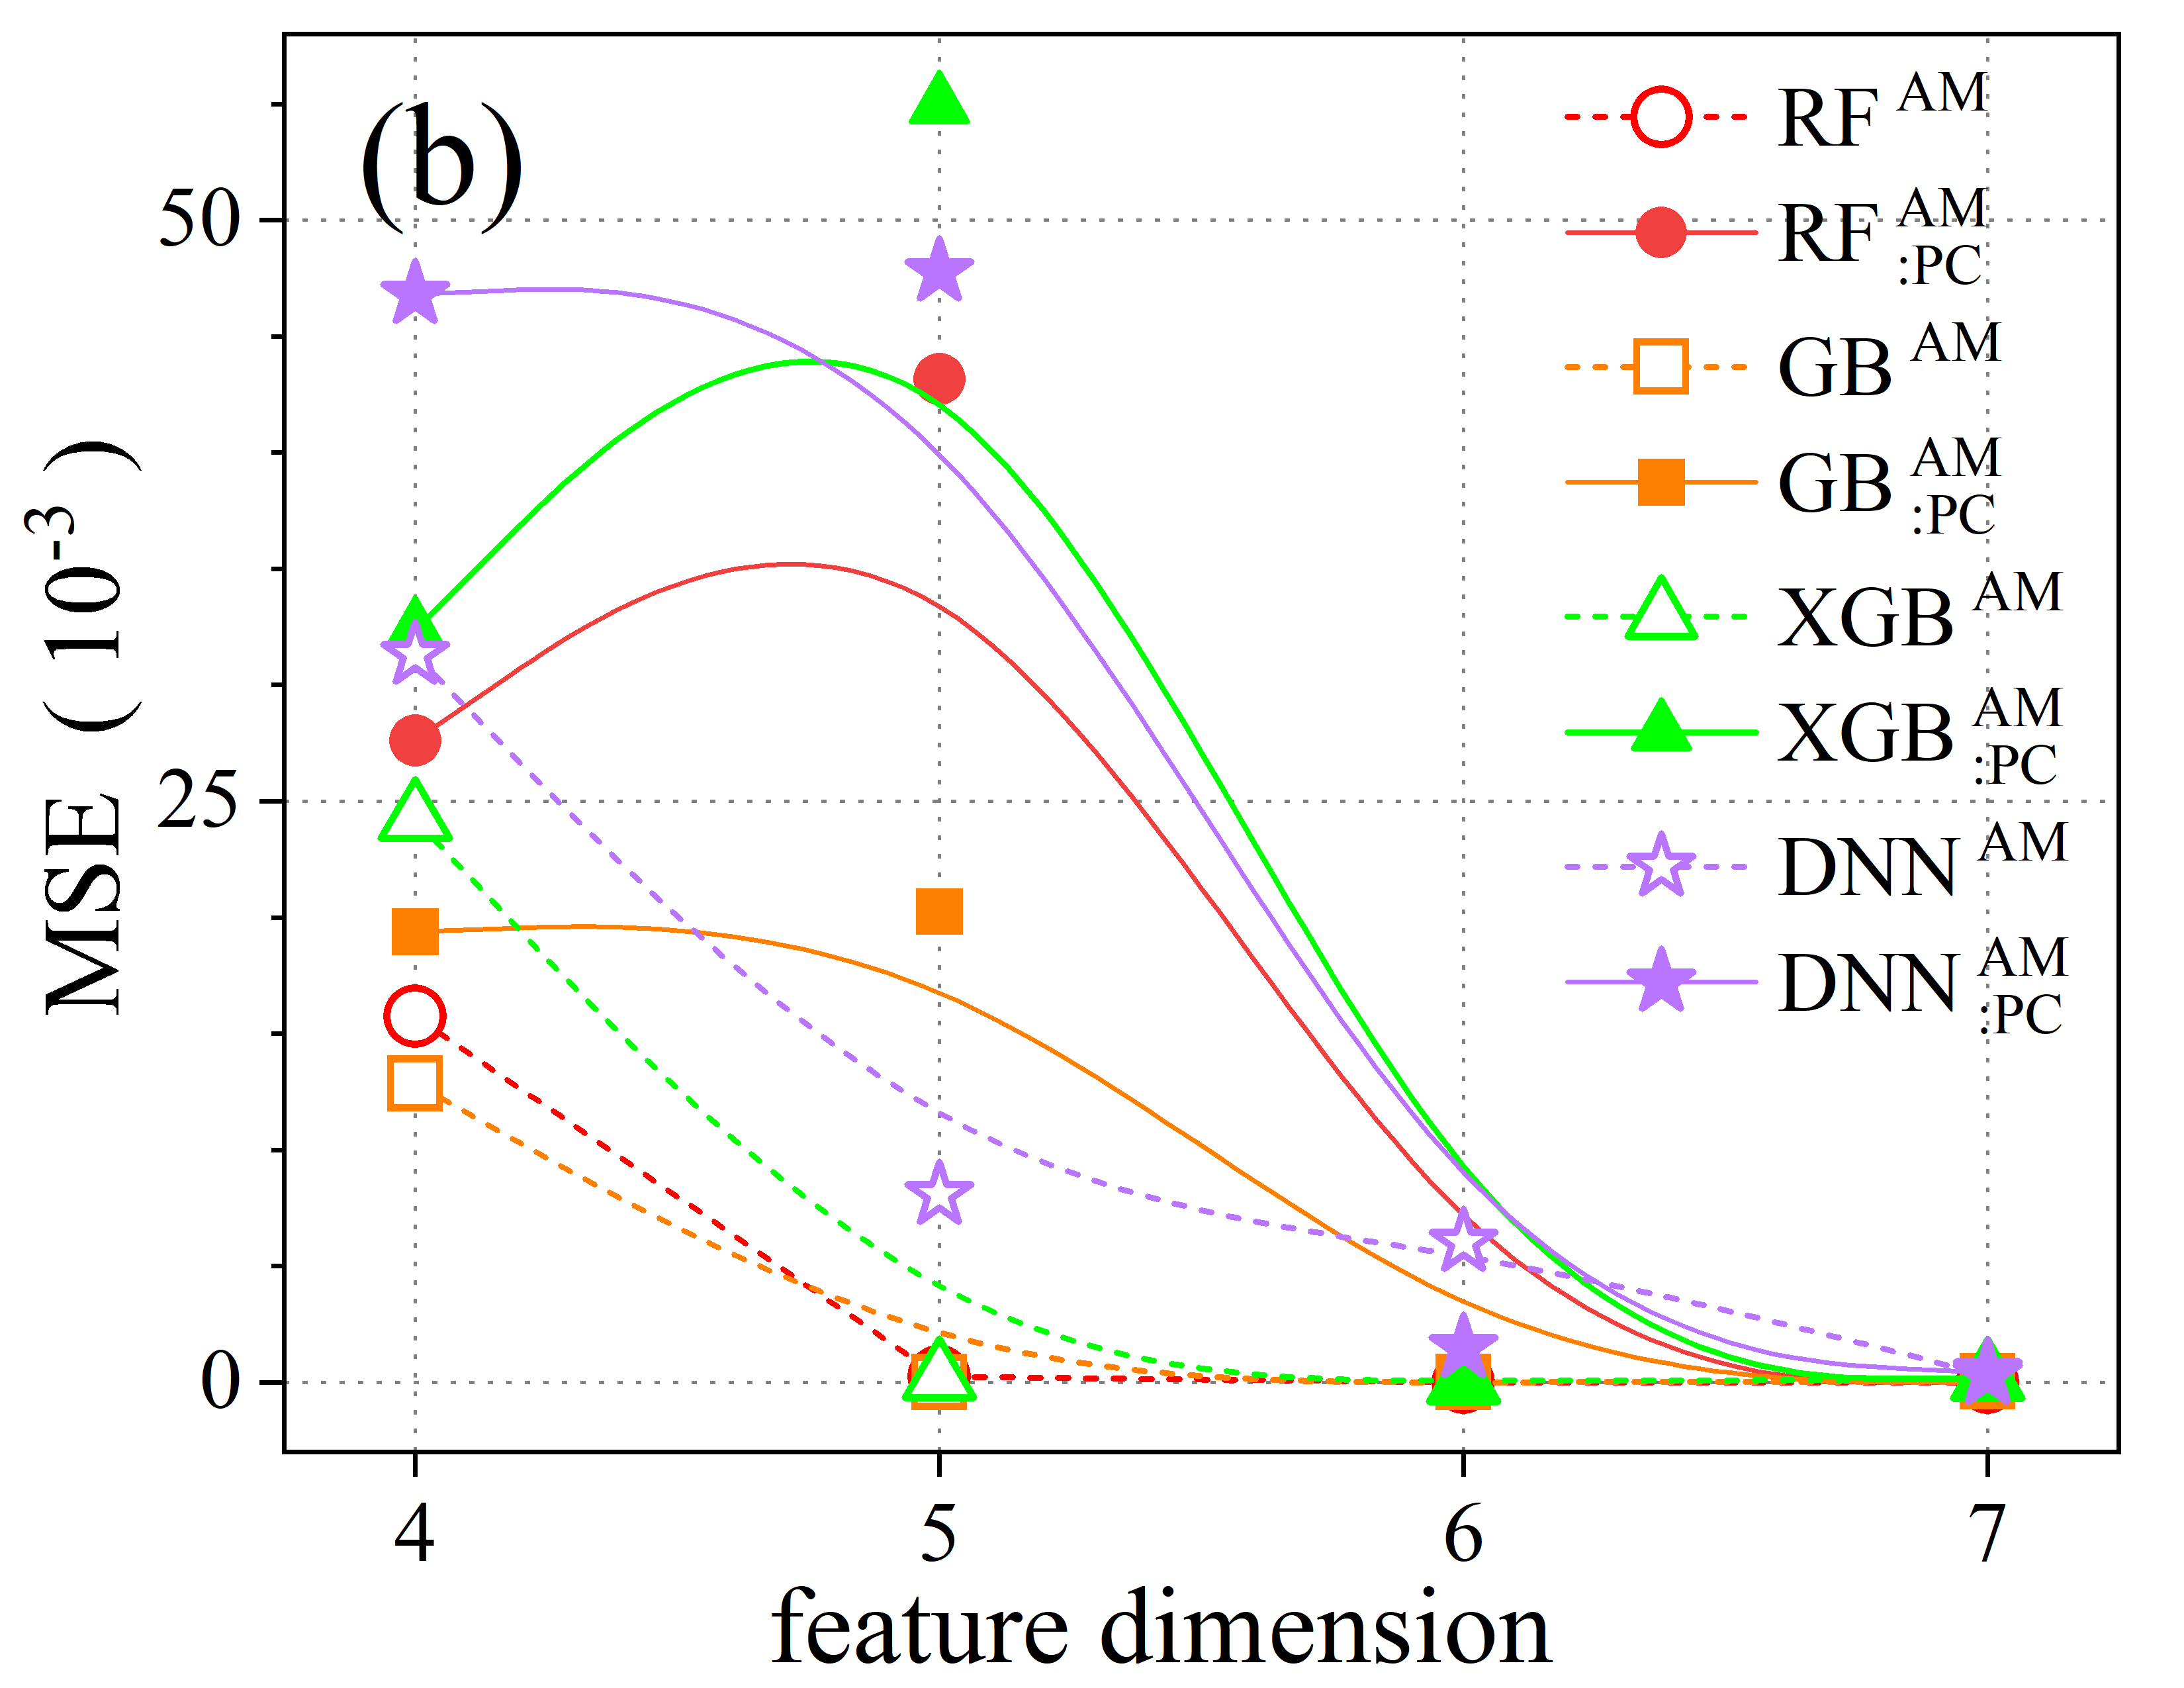
\includegraphics[width=0.4\linewidth]{Fig4b.png}
	  \caption{MSE dependence on input feature dimension for training data obtained under monochromatic (a) and AM1.5 illumination (b).
ML algorithms: RF (circles), GB (rectangles), XGB (triangles), and DNN (stars).
Closed markers indicate results with PCA, while open markers represent results without PCA.
}\label{fig4}
\end{figure}

Fig.~\ref{fig5} illustrates typical dependencies of the proportion of predictions with
a given accuracy on $T$, $d_p$, $N_\mathrm{B}$, and $N_\mathrm{Fe}$),
enabling an assessment of the models' predictive capabilities based on measurement conditions, solar cell structure, and iron concentration.
The data indicate that the most challenging cases for prediction involve $N_\mathrm{Fe}<10^{11}$~cm$^{-3}$
and solar cells with a base doping level around $10^{16}$~cm$^{-3}$.
The last difficulty arises because, as shown by simulation \cite{Olikh2025MSEB},
variations in PV parameters during FeB pair dissociation remain minimal.
Meanwhile, measurement temperature and base thickness (when feature dimensionality exceeds 4) have virtually no impact on prediction accuracy.

\begin{figure}
  \centering
     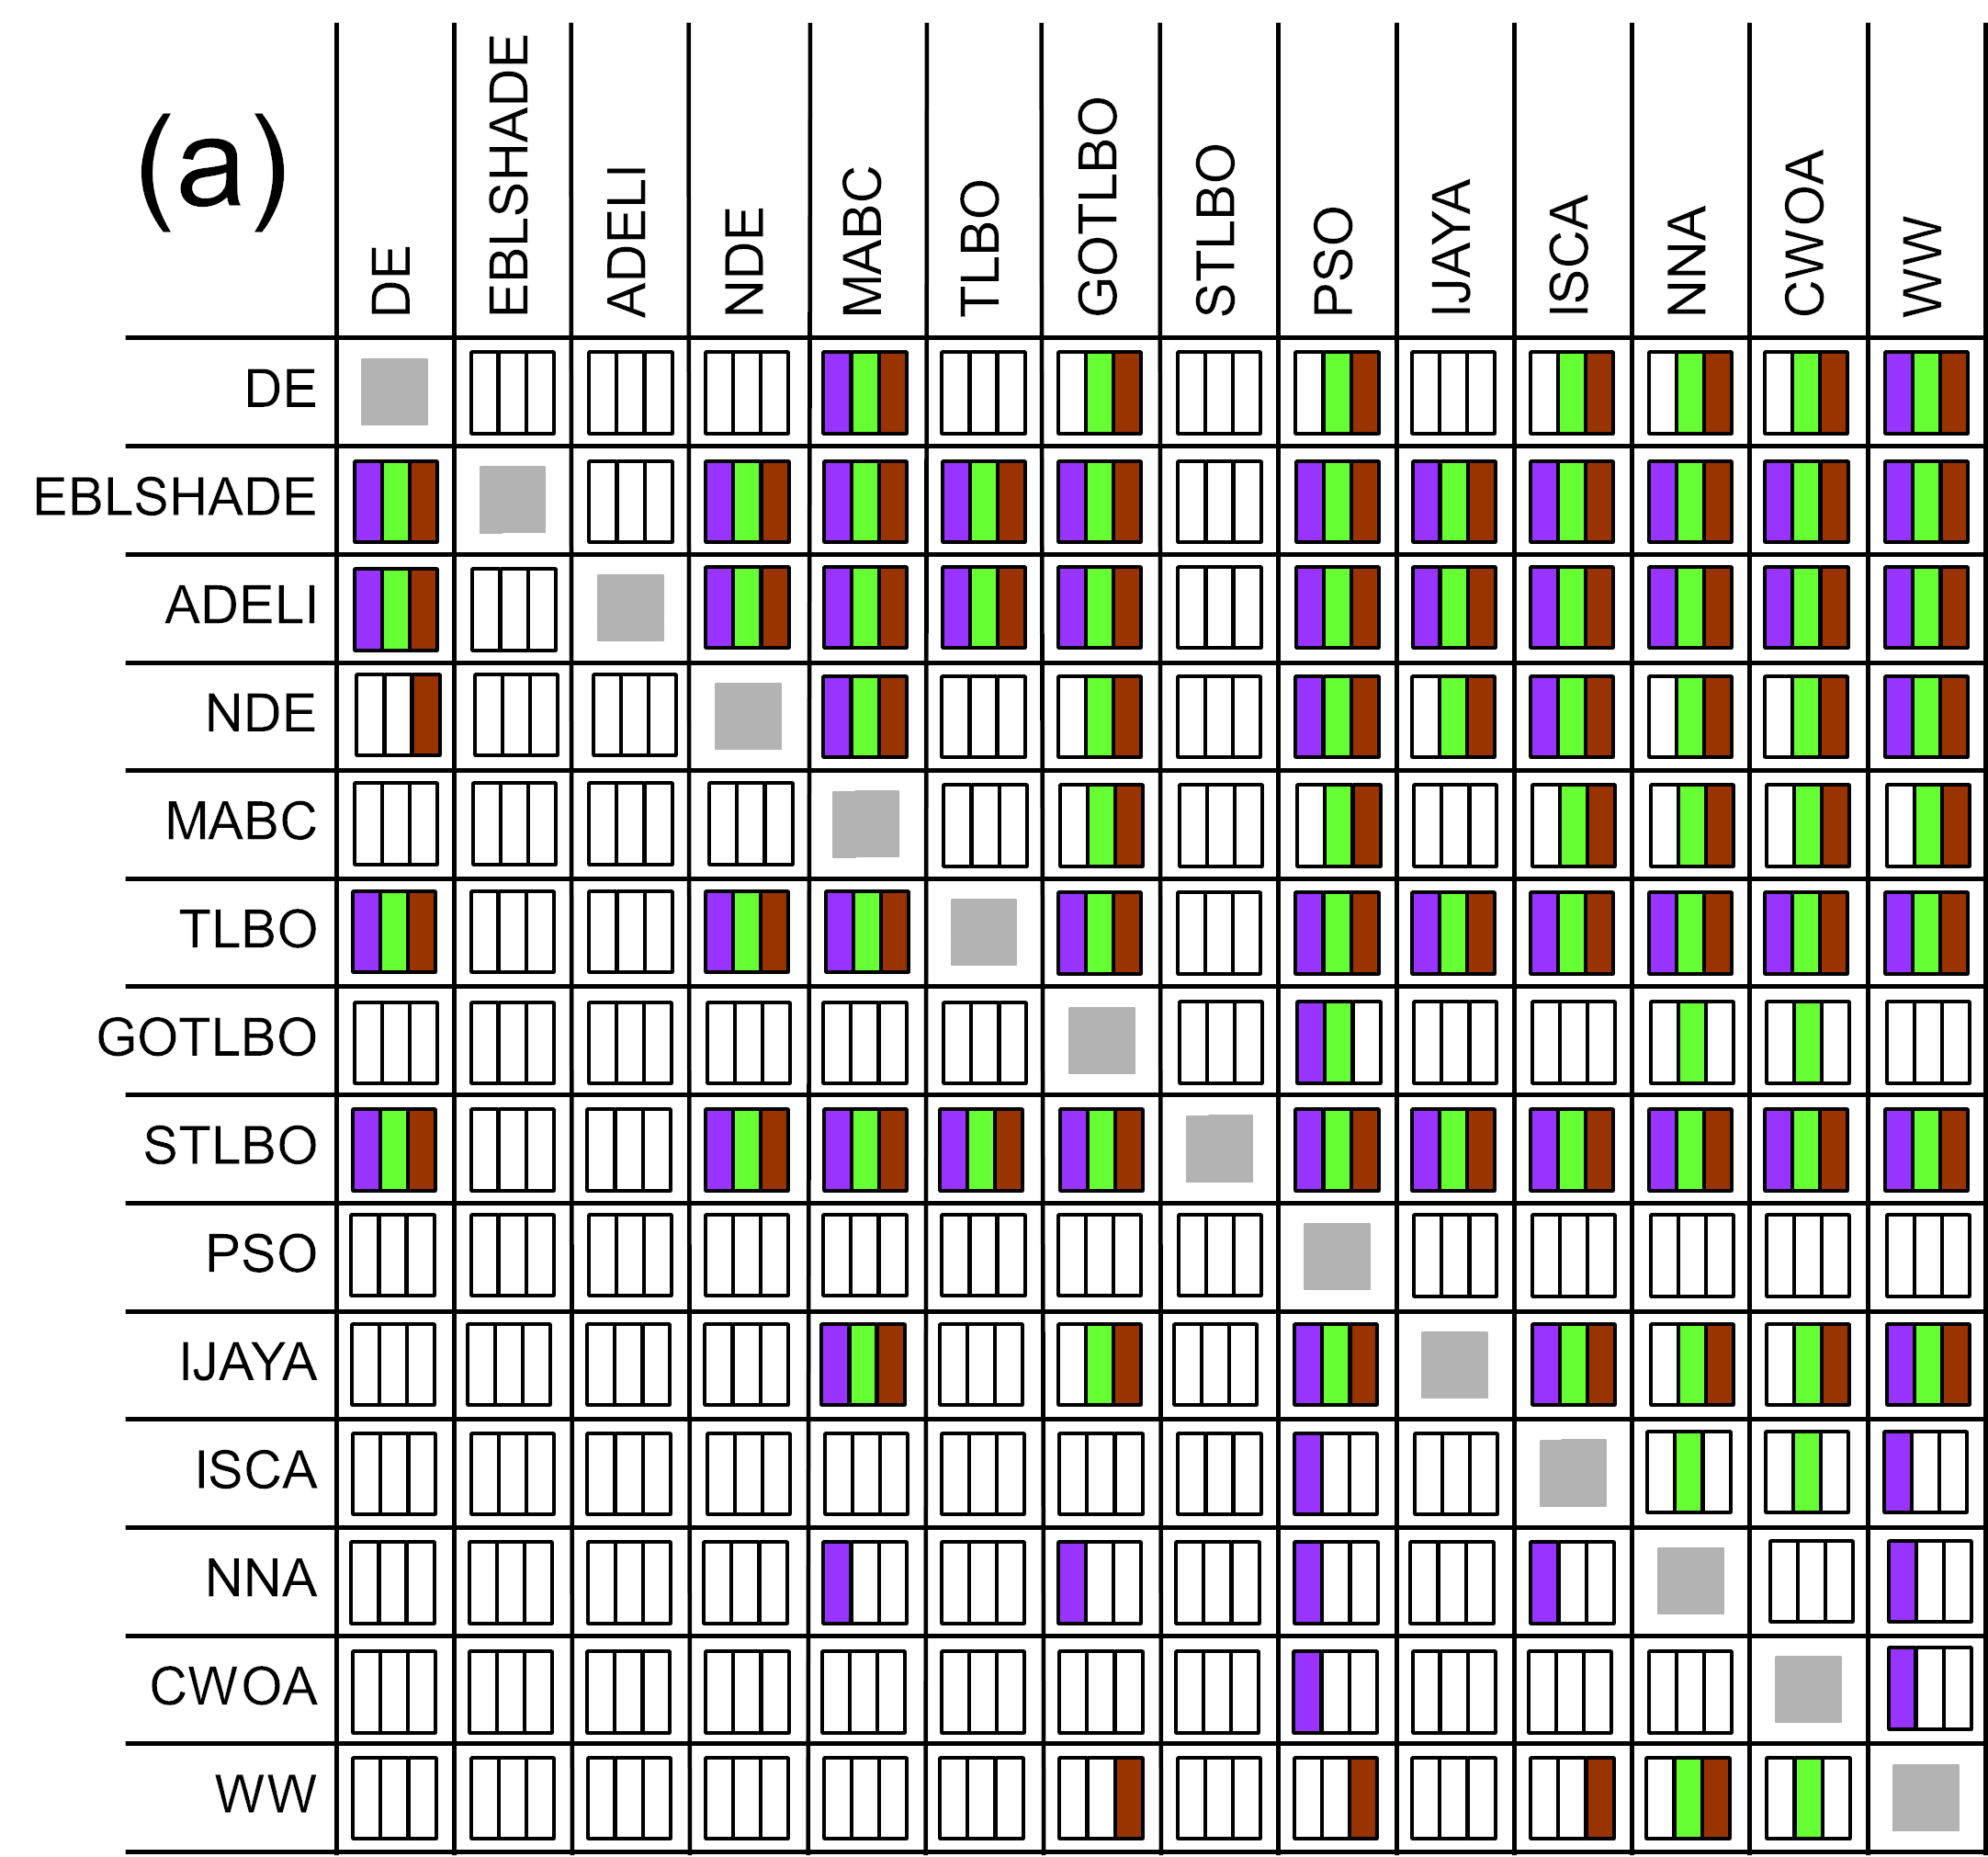
\includegraphics[width=0.4\linewidth]{Fig5a.png}
     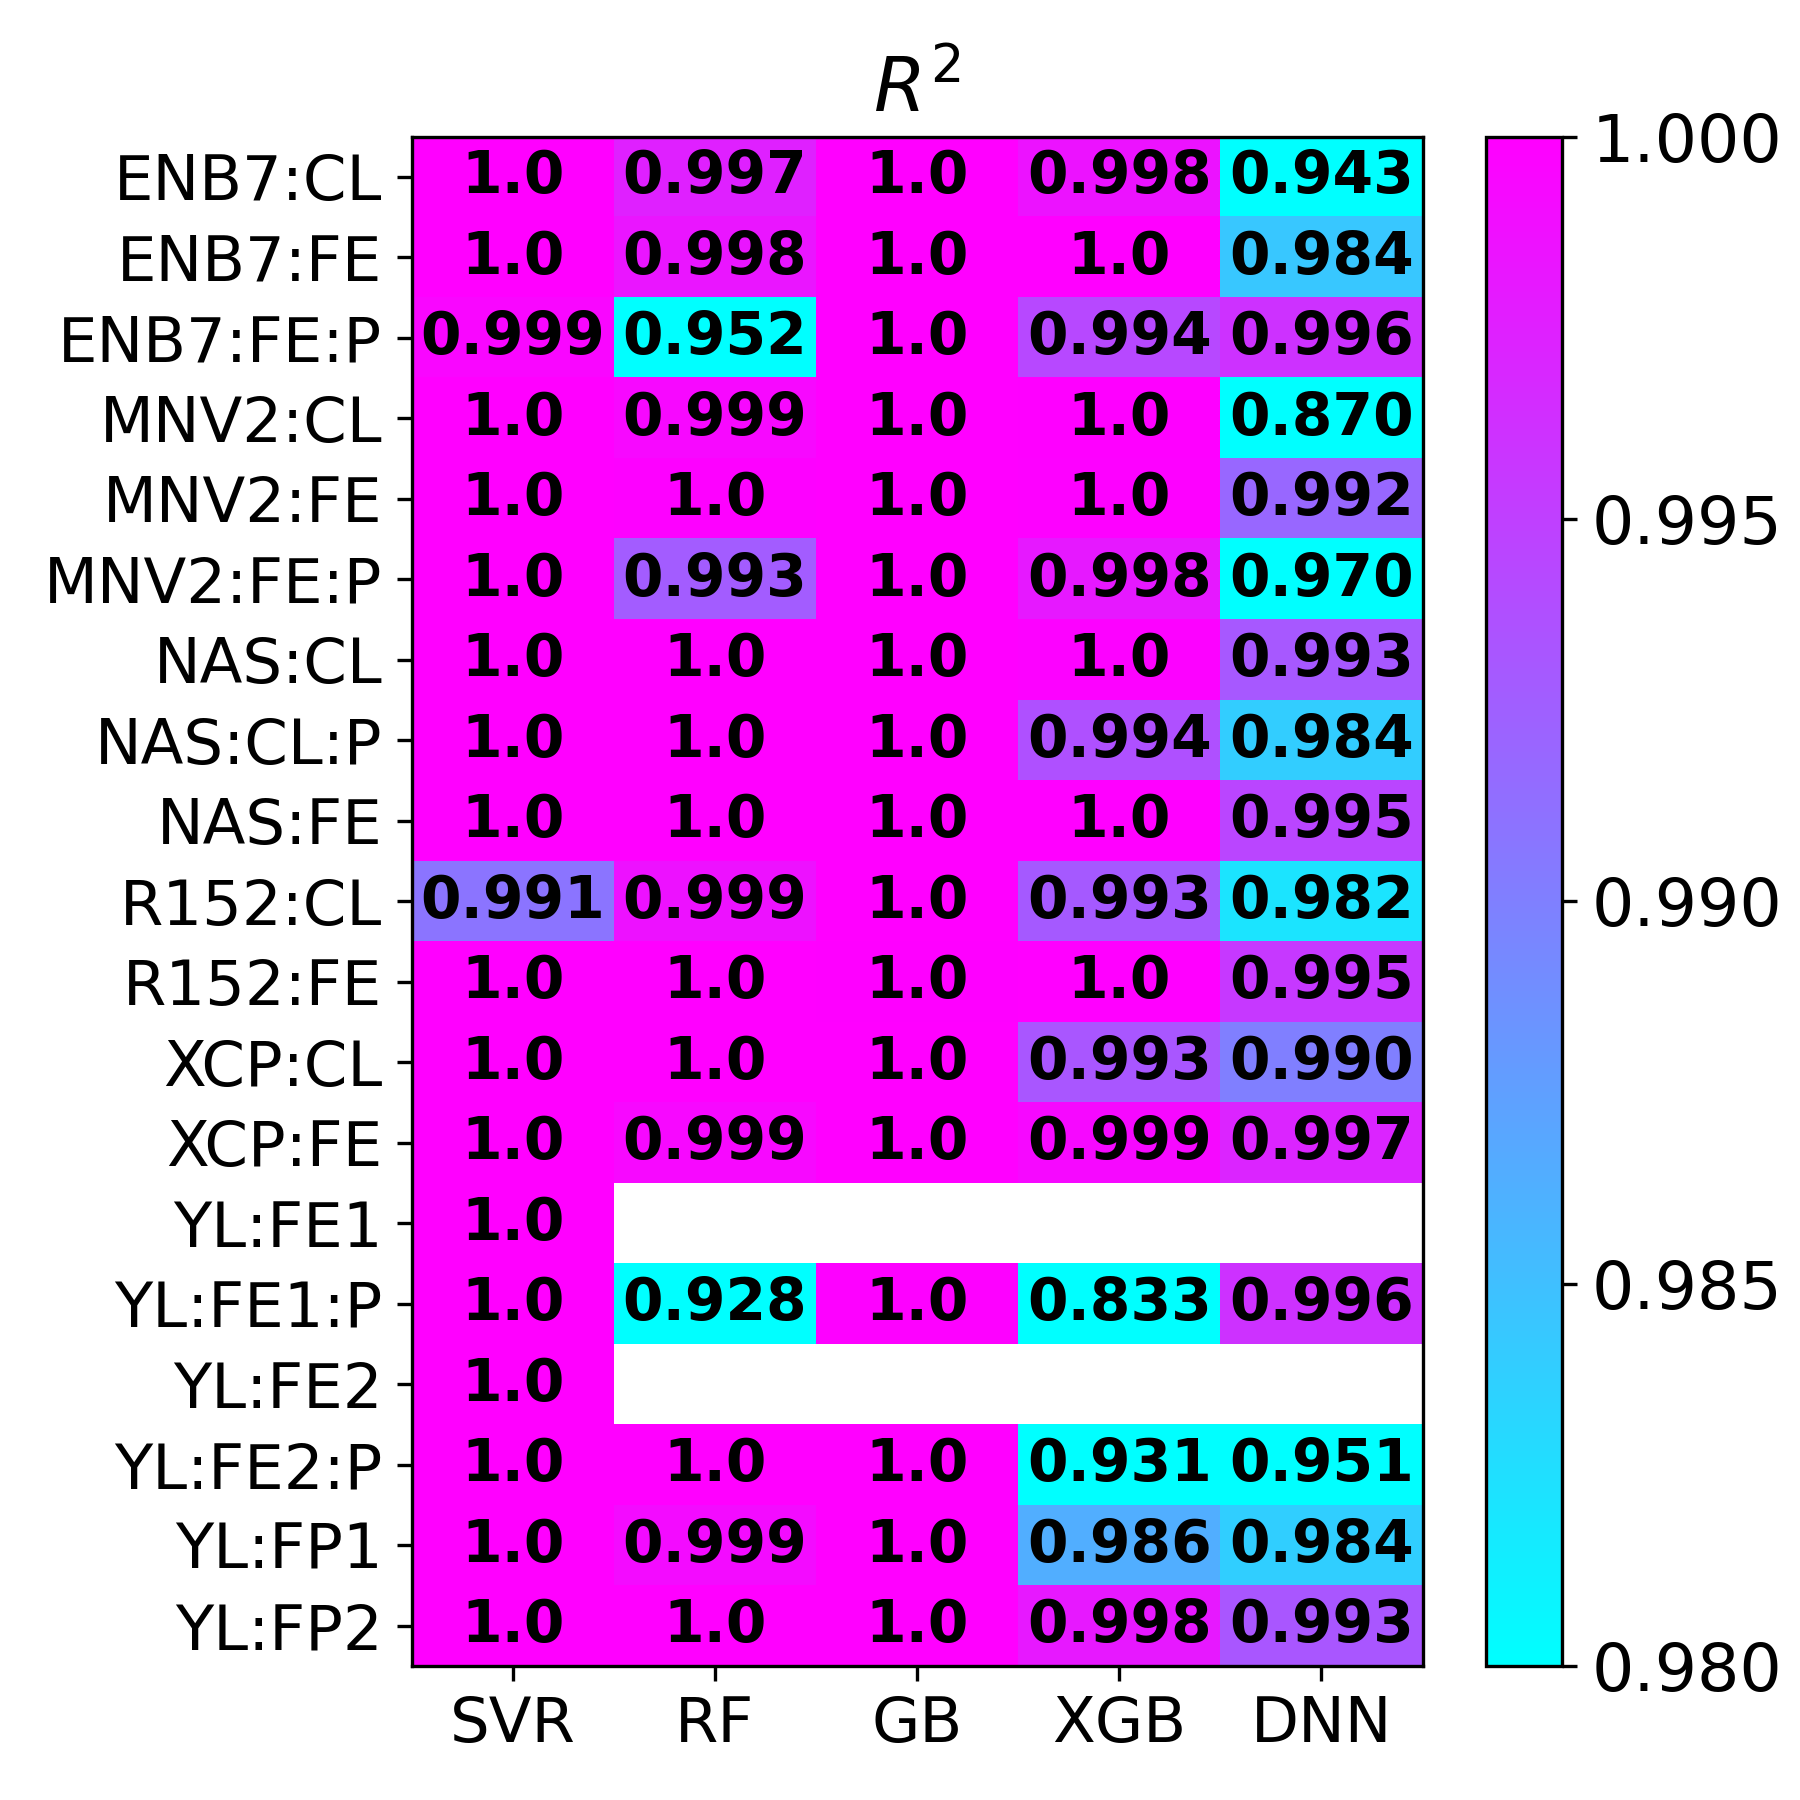
\includegraphics[width=0.4\linewidth]{Fig5b.png}
     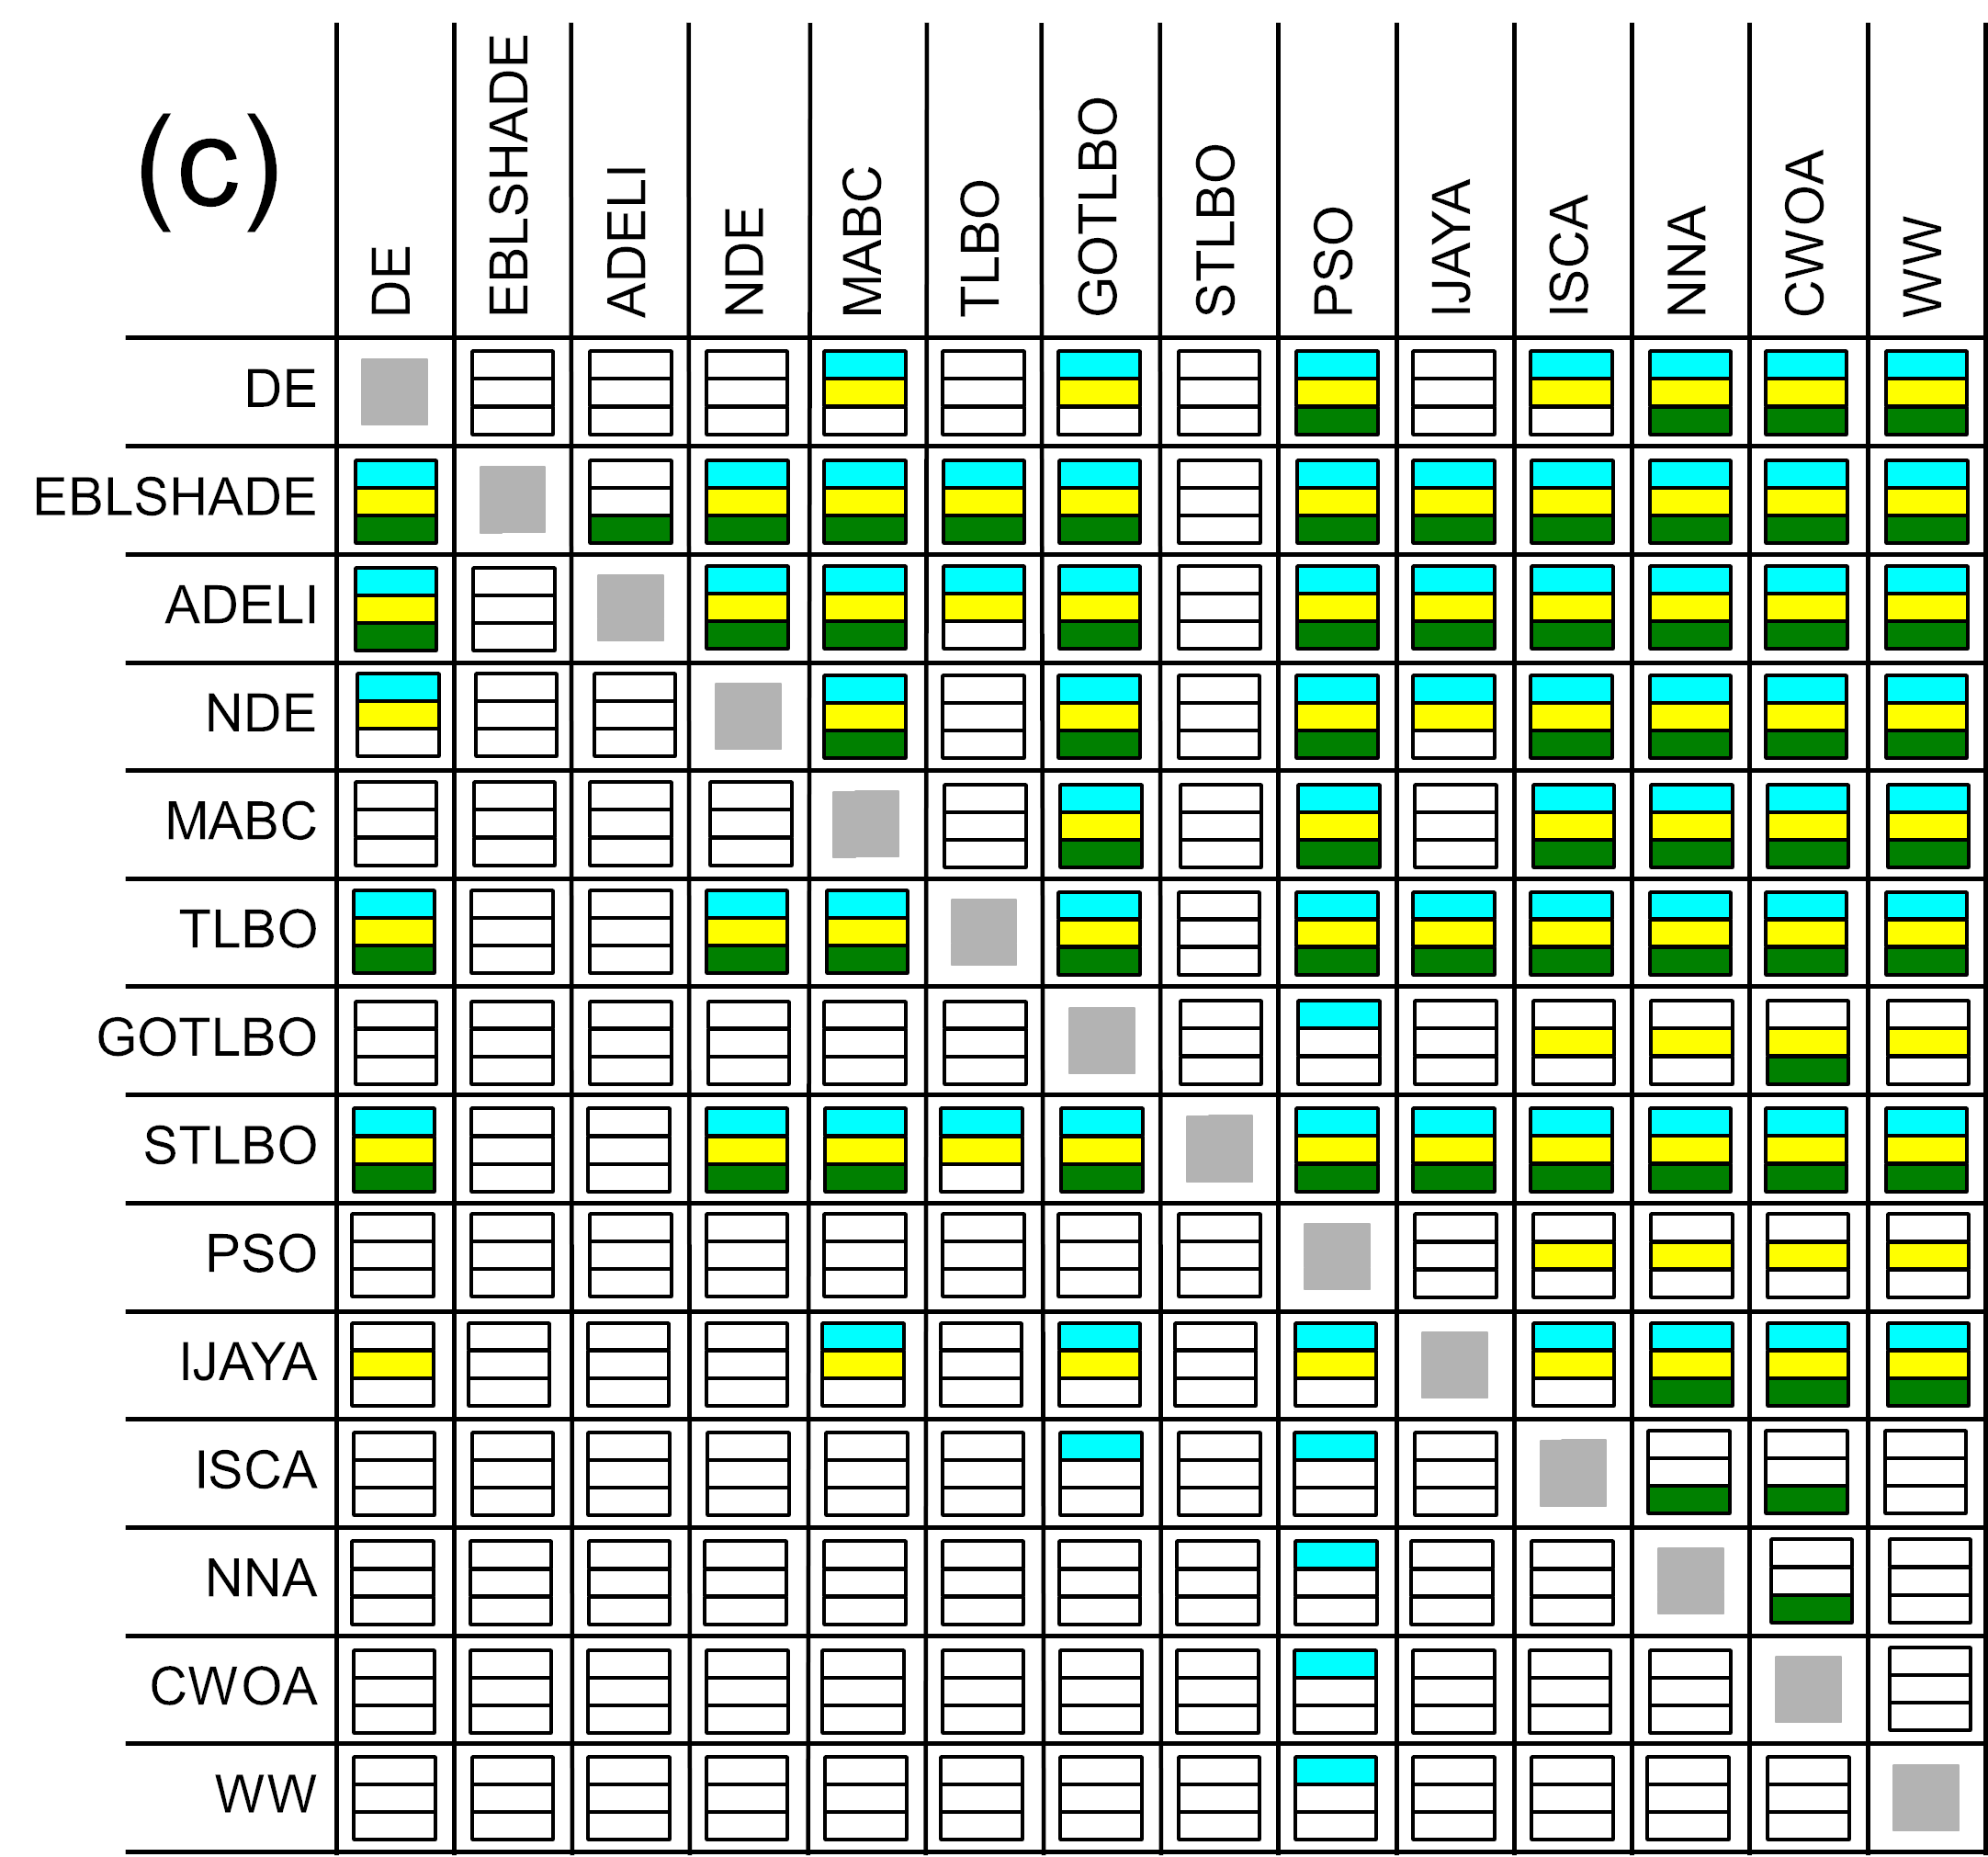
\includegraphics[width=0.4\linewidth]{Fig5c.png}
     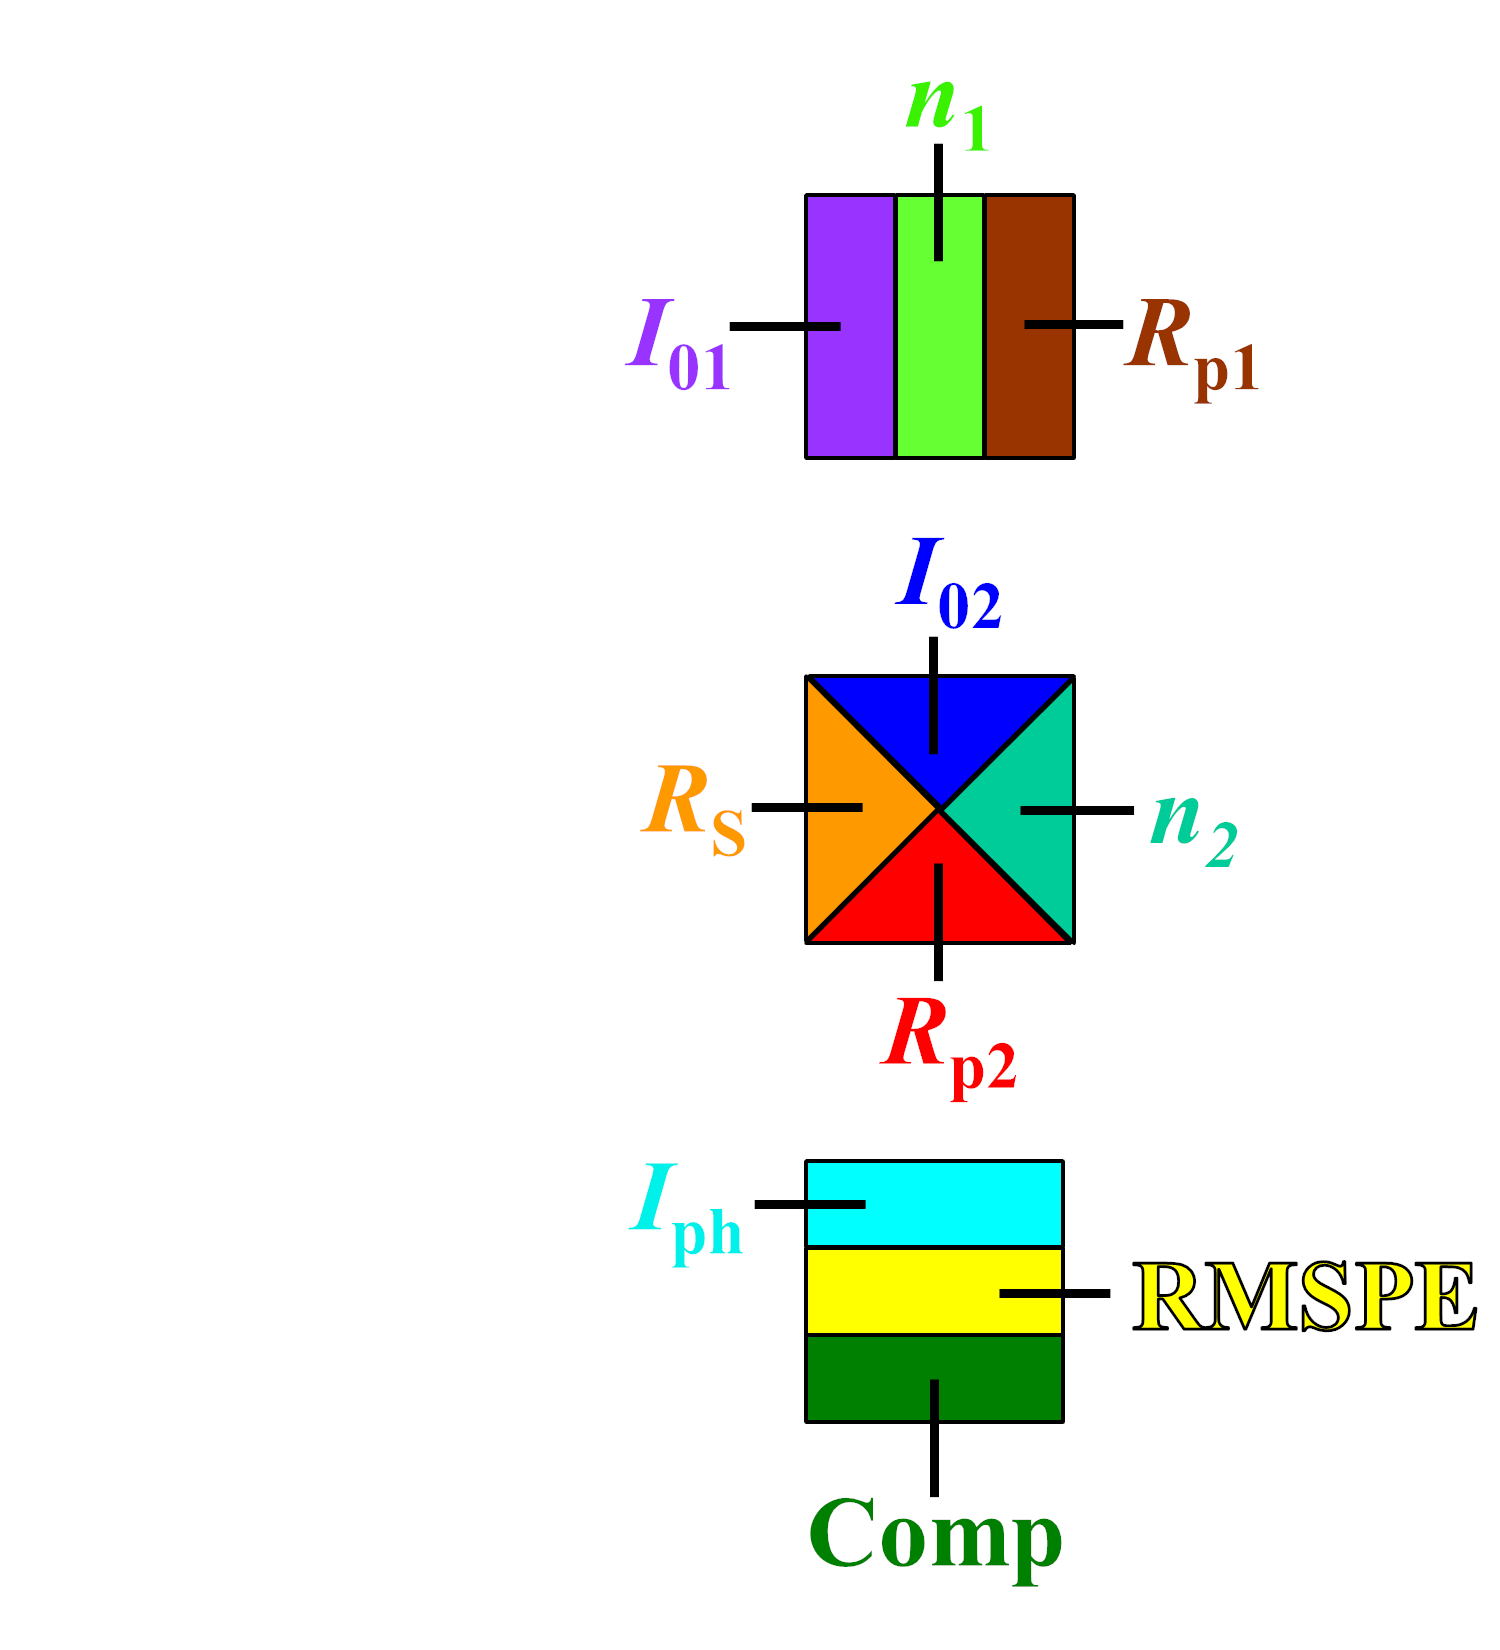
\includegraphics[width=0.4\linewidth]{Fig5d.png}
    \caption{Typical dependencies of the proportion of predictions with an accuracy of at least 10\%
    (a, b, c) or 1\% (d) on iron concentration, alloying level, substrate thickness, and temperature.
}\label{fig5}
\end{figure}

\subsection{$N_\mathrm{Fe}$--altered test dataset}

The $N_\mathrm{Fe}$--altered test dataset is the most realistic,
as it mimics real-world conditions where the goal is to predict iron concentration based
on PVP variations measured under standardized conditions for predefined structures,
using the same temperature and solar cell parameters as in model training.


Fig.~\ref{fig6} and \textcolor[rgb]{1.00,0.07,0.00}{
\hl{Figs.}}~S8--S11 in Supplementary Materials present the prediction results,
while Fig.~\ref{fig7} and Table~\ref{table2} summarize the performance metrics.
SVR consistently performs poorly, a trend observed across all test datasets.
Since this pattern remains unchanged in subsequent analyses, we do not discuss it further.
For the remaining models, it is crucial to differentiate between results obtained under monochromatic and solar illumination.
Under 940~nm illumination without PCA, nearly all algorithms achieve reasonably accurate predictions, with a MAPE of approximately 10\textcolor[rgb]{1.00,0.07,0.00}{
\hl{\%.}}
DNN models yield slightly worse results, whereas XGB demonstrates marginally better performance.
Interestingly, increasing feature dimensionality does not improve prediction accuracy but instead reduces it.
Notably, incorporating the relative changes in the fill factor into the descriptor set significantly degrades DNN predictions.
As shown in Table~\ref{table2}, RF, GB, and XGB, which are the most accurate models, exhibit a noticeable increase
in MdAPE and a rise in $p01$ and $p10$ as the number of descriptors grows.
These trends indicate that expanding feature dimensionality leads to a higher proportion of predictions with significant errors,
as illustrated in Fig.~\ref{fig8}a for GB.
Fig.~\ref{fig8}a and Table~\ref{table2} also show that PCA-based model simplification increases the proportion of high--error predictions
in XGB while reducing it in RF and GB.
In summary, $\mathrm{GB}^{940}_\mathrm{4:PC}$, $\mathrm{GB}^{940}_\mathrm{5:PC}$,
and $\mathrm{XGB}^{940}_5$ yield the most precise results for this test dataset under monochromatic illumination,
with the proportion of predictions achieving at least 10\% accuracy reaching 80.3\%, 82.4\%, and 78.6\%, respectively.


\begin{figure}
	\centering
     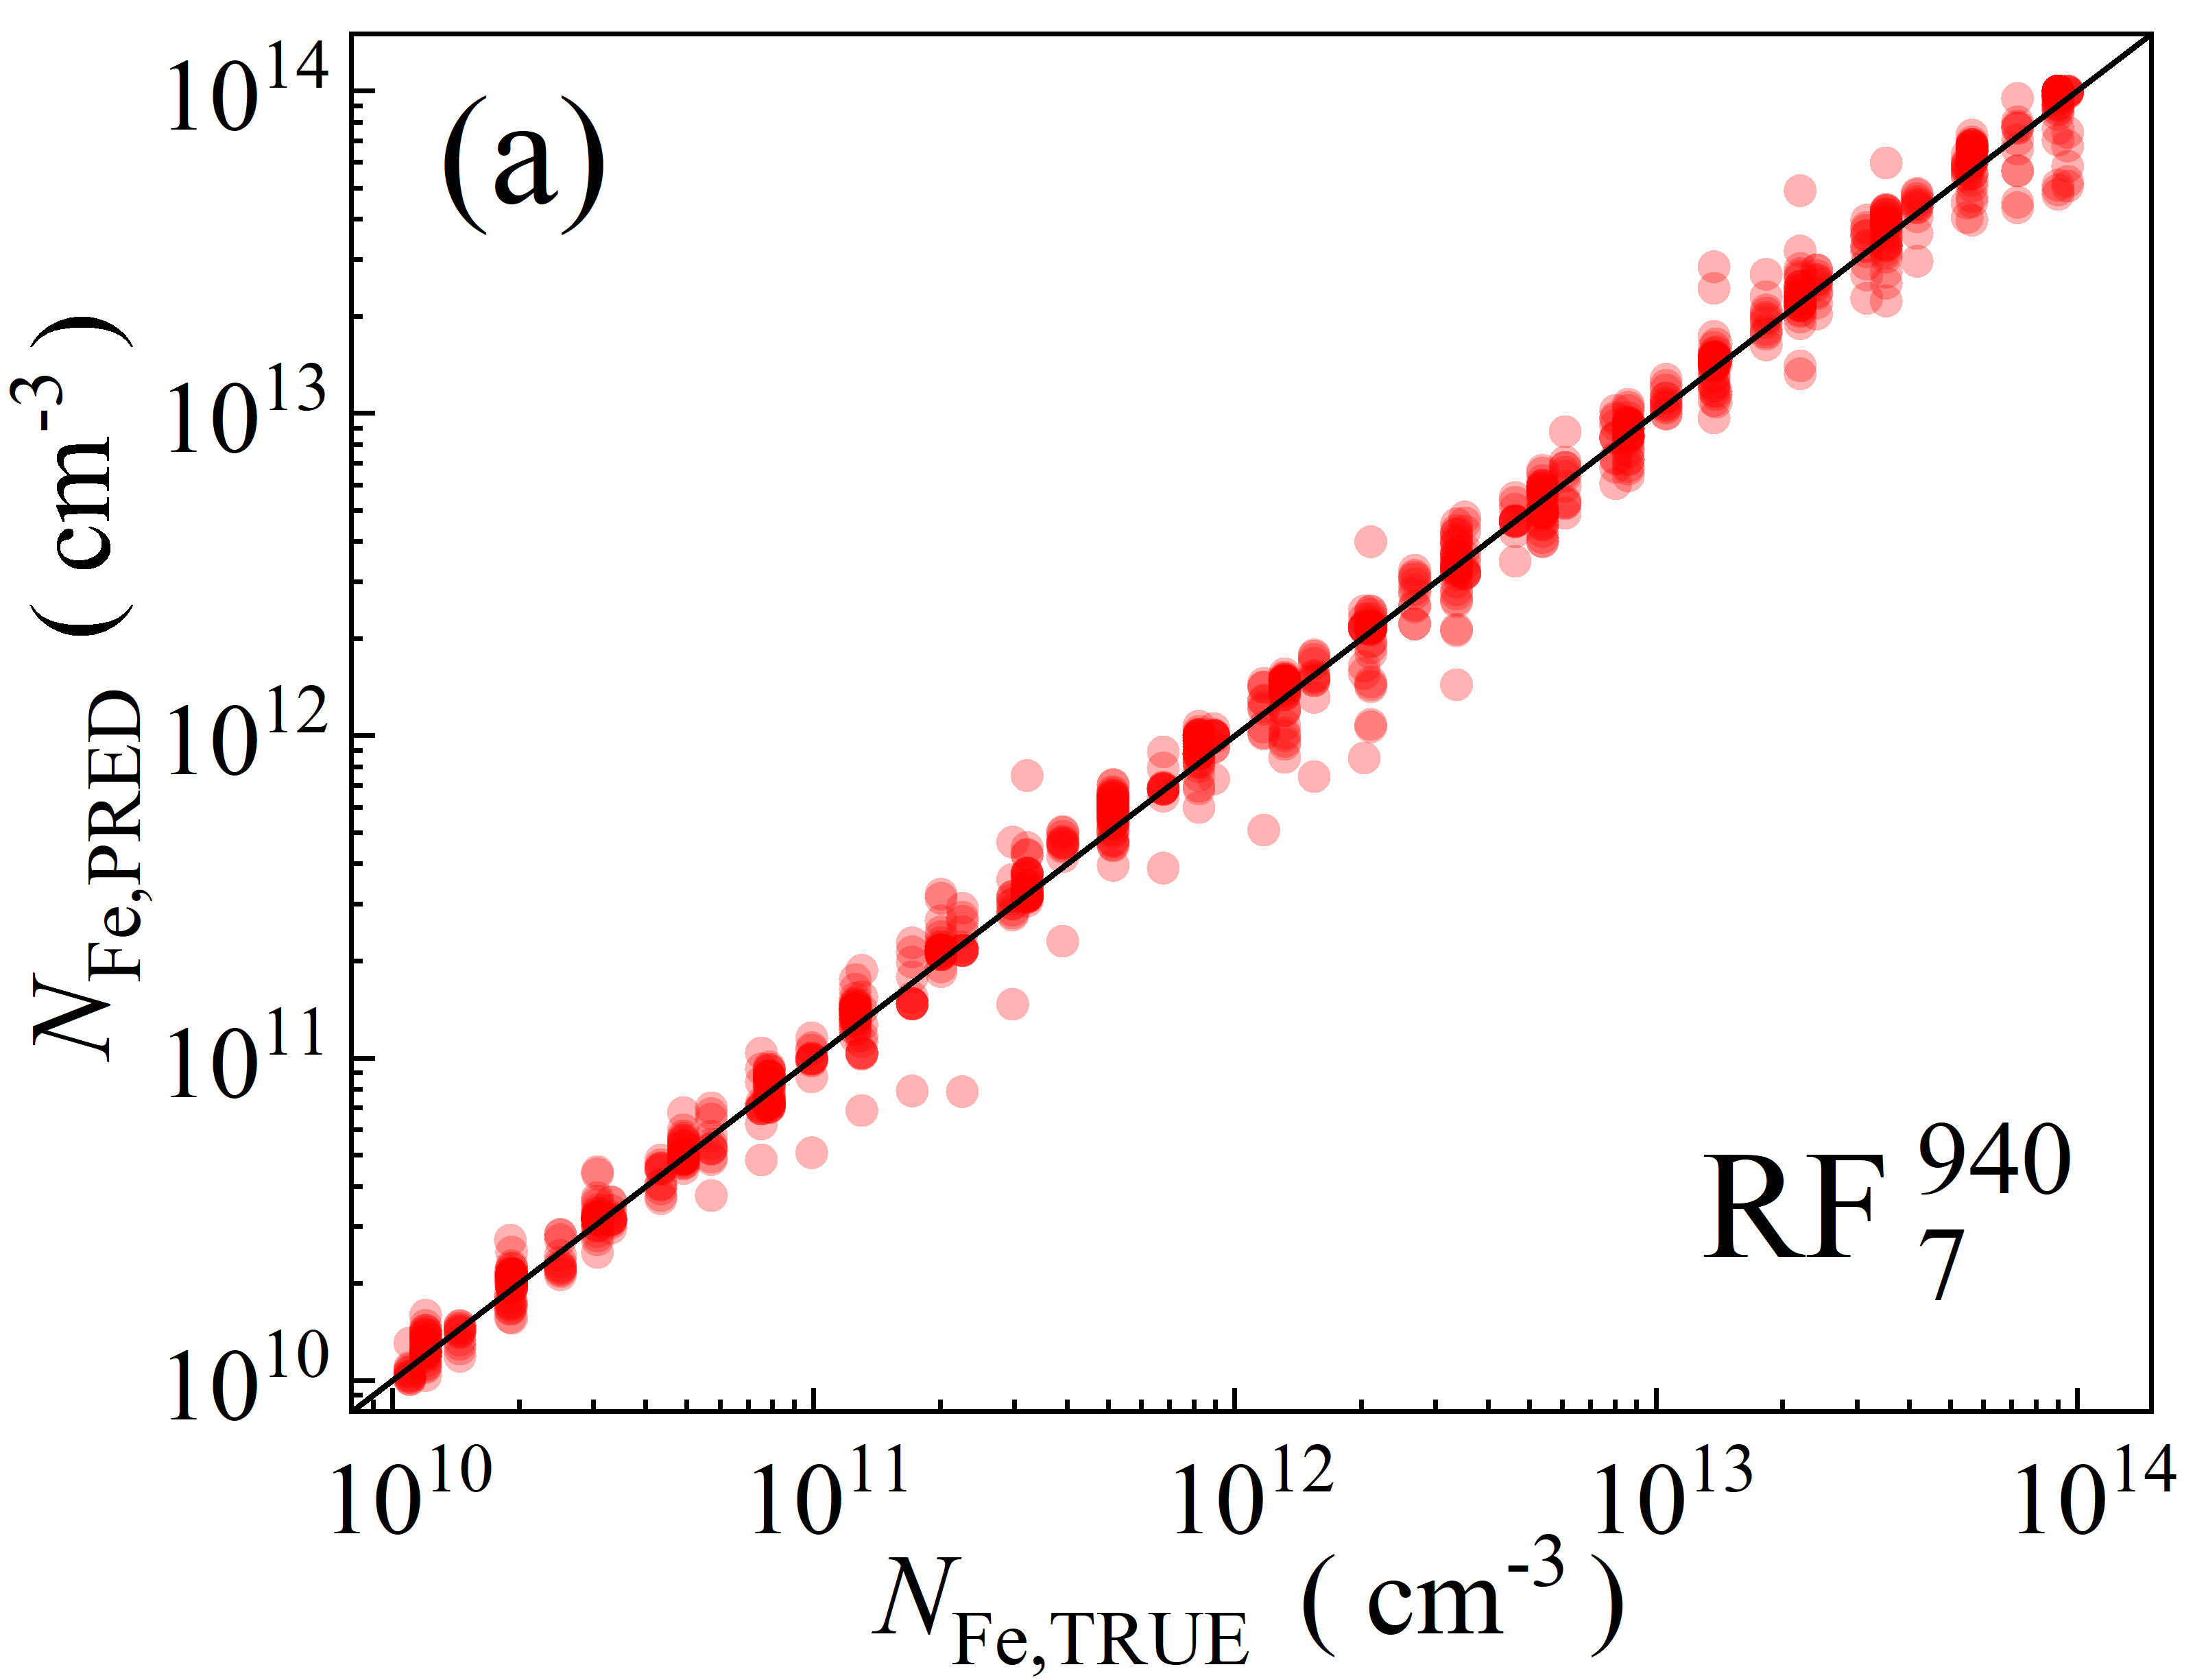
\includegraphics[width=0.24\linewidth]{Fig6a.png}
     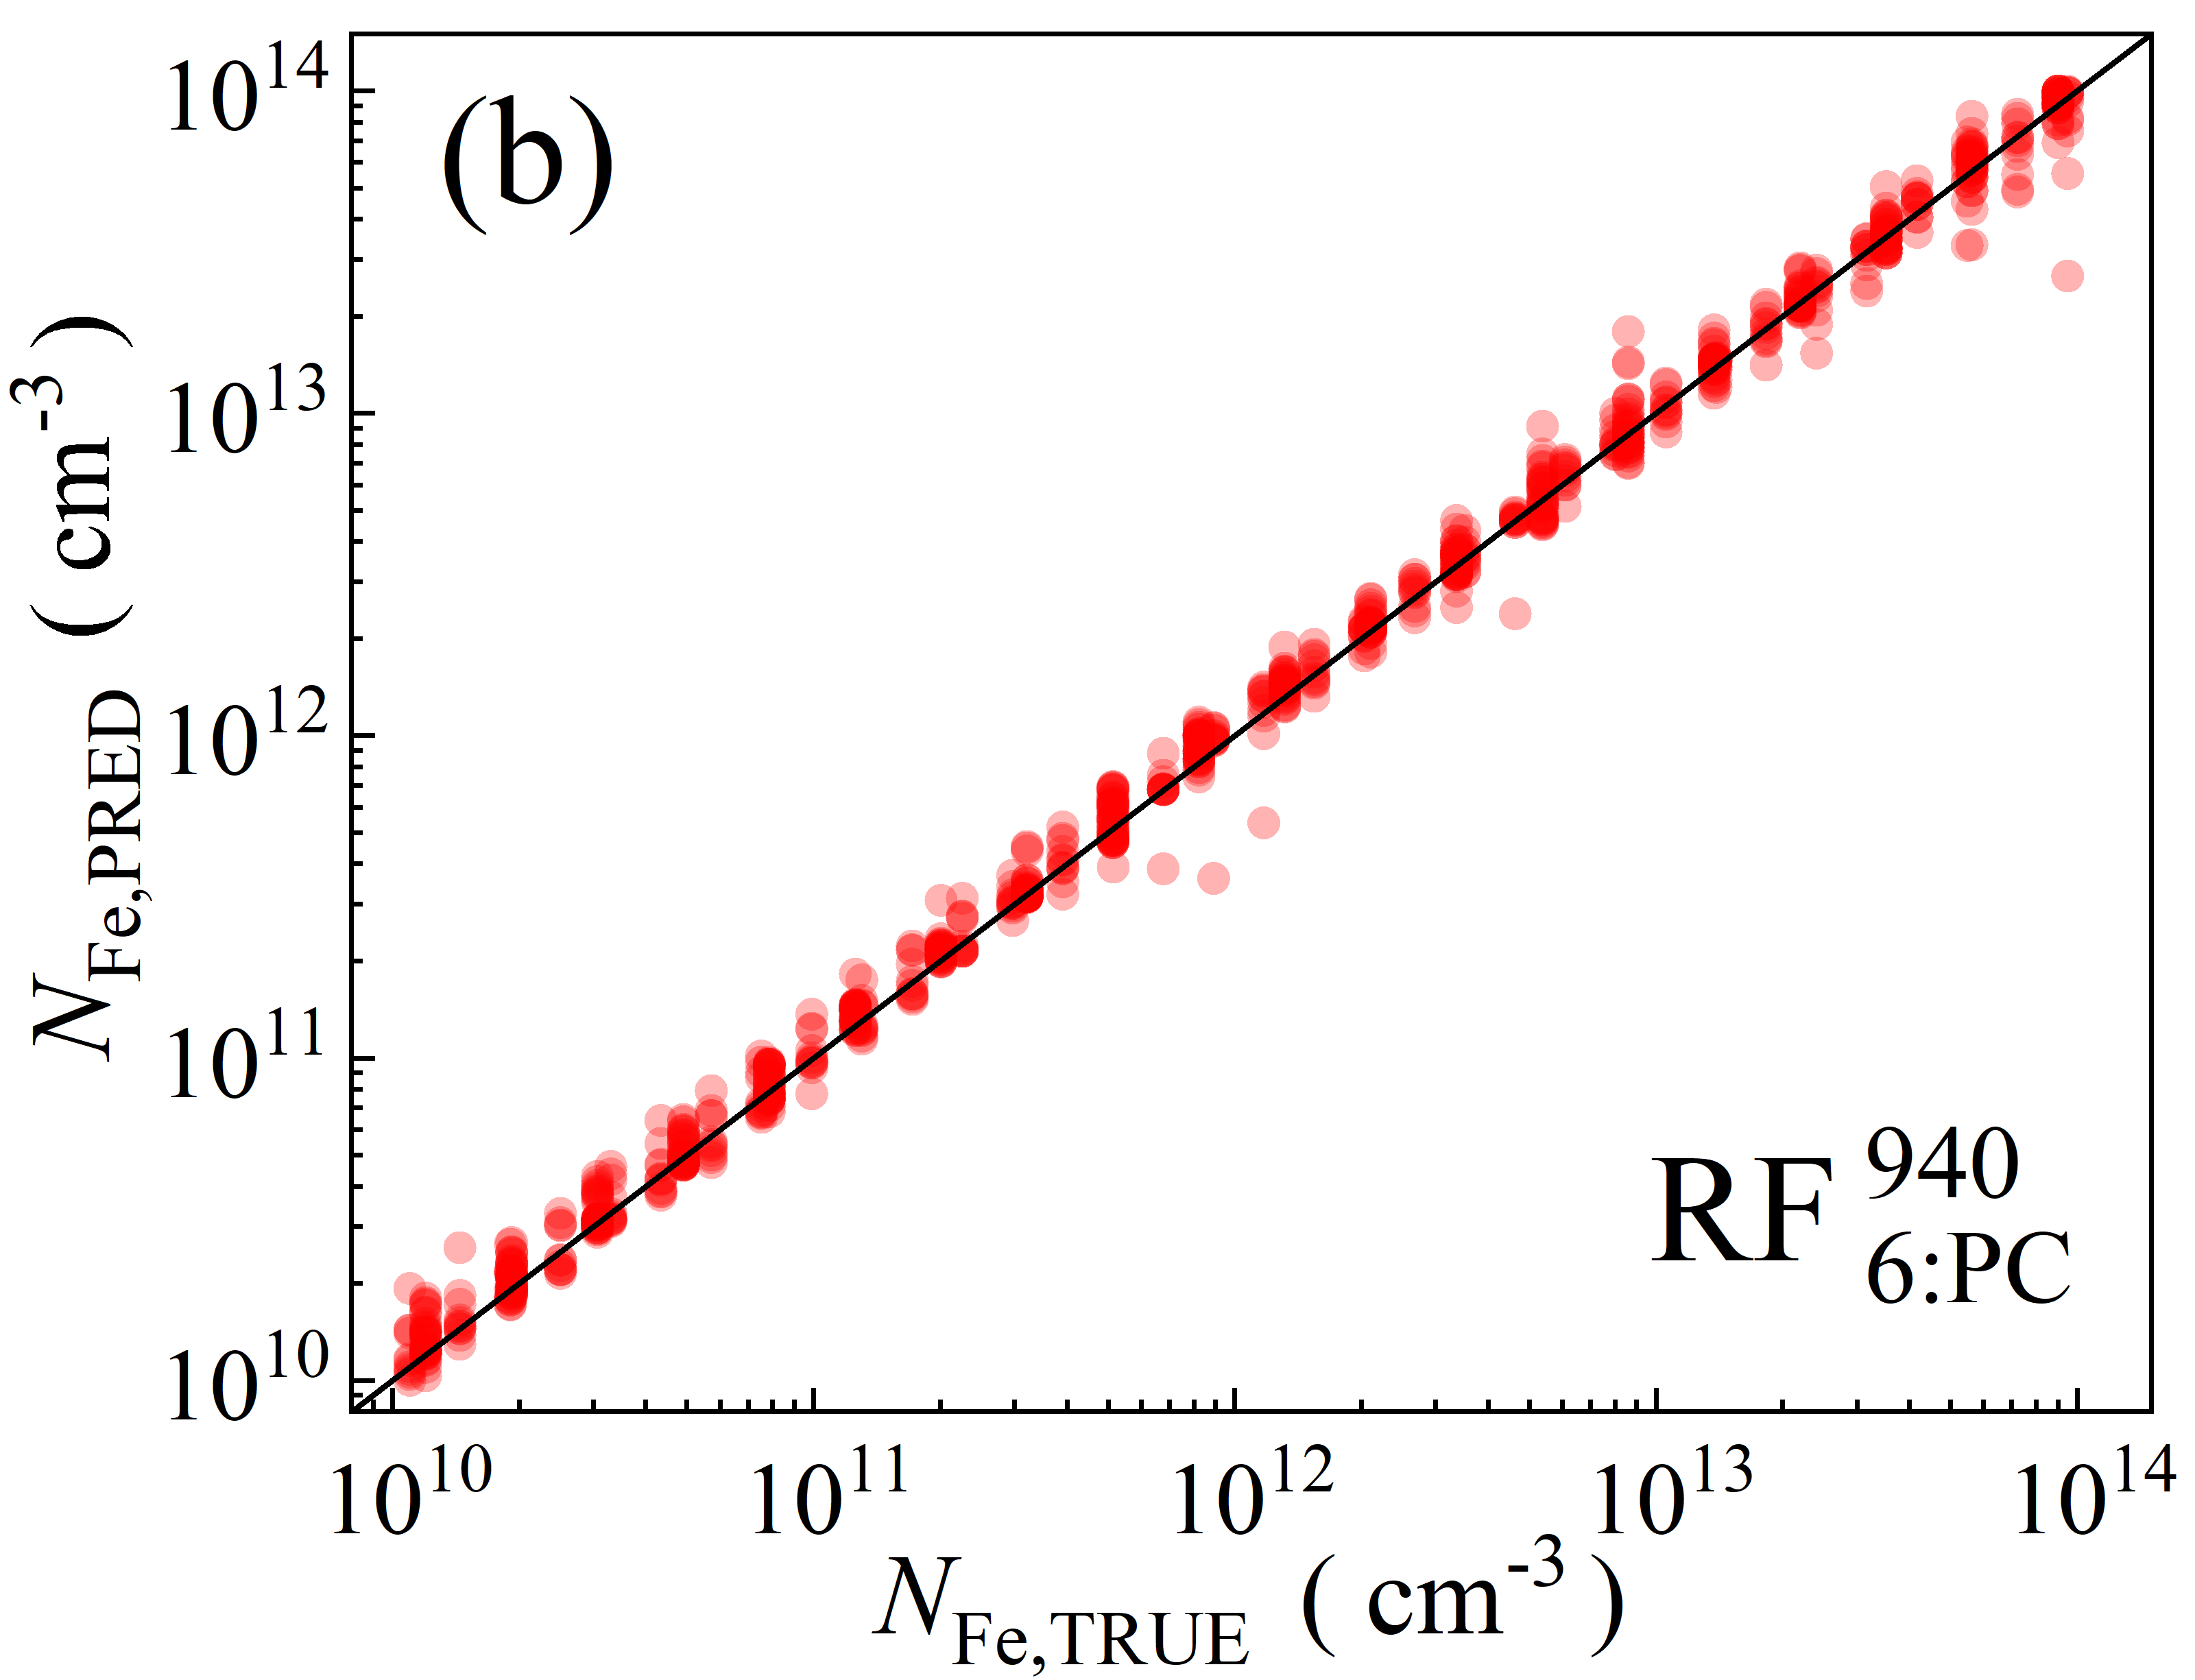
\includegraphics[width=0.24\linewidth]{Fig6b.png}
     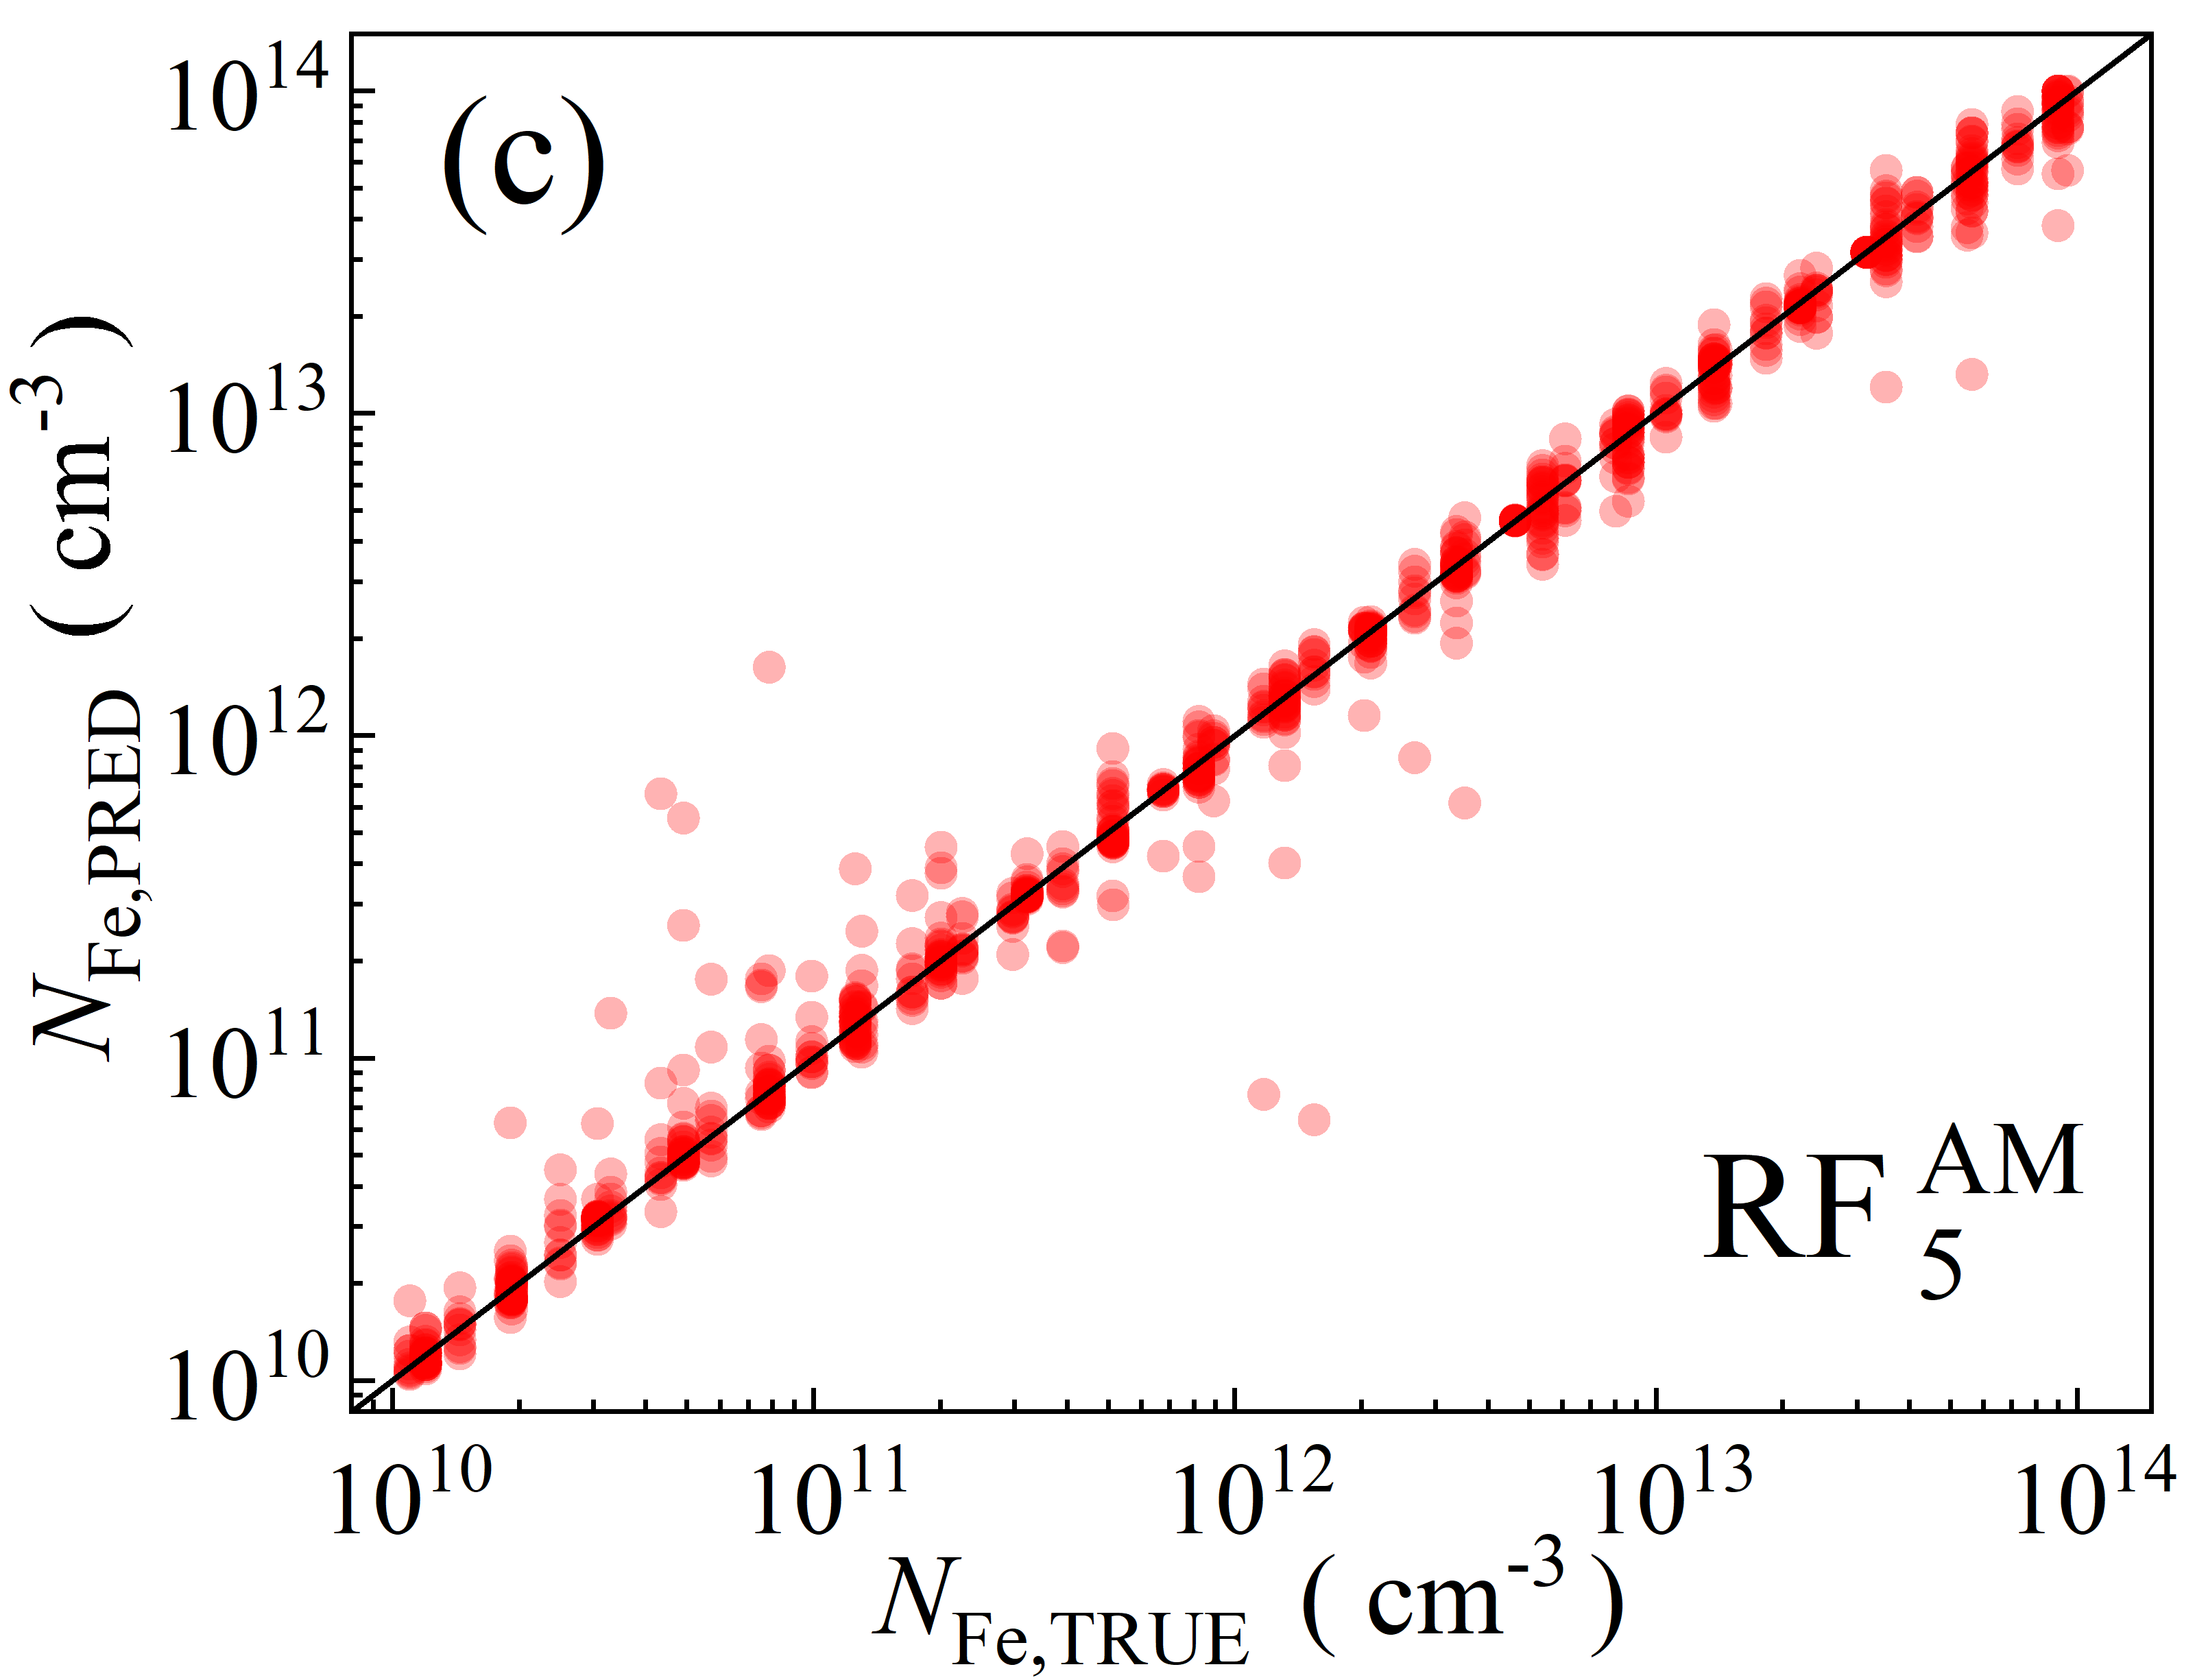
\includegraphics[width=0.24\linewidth]{Fig6c.png}
     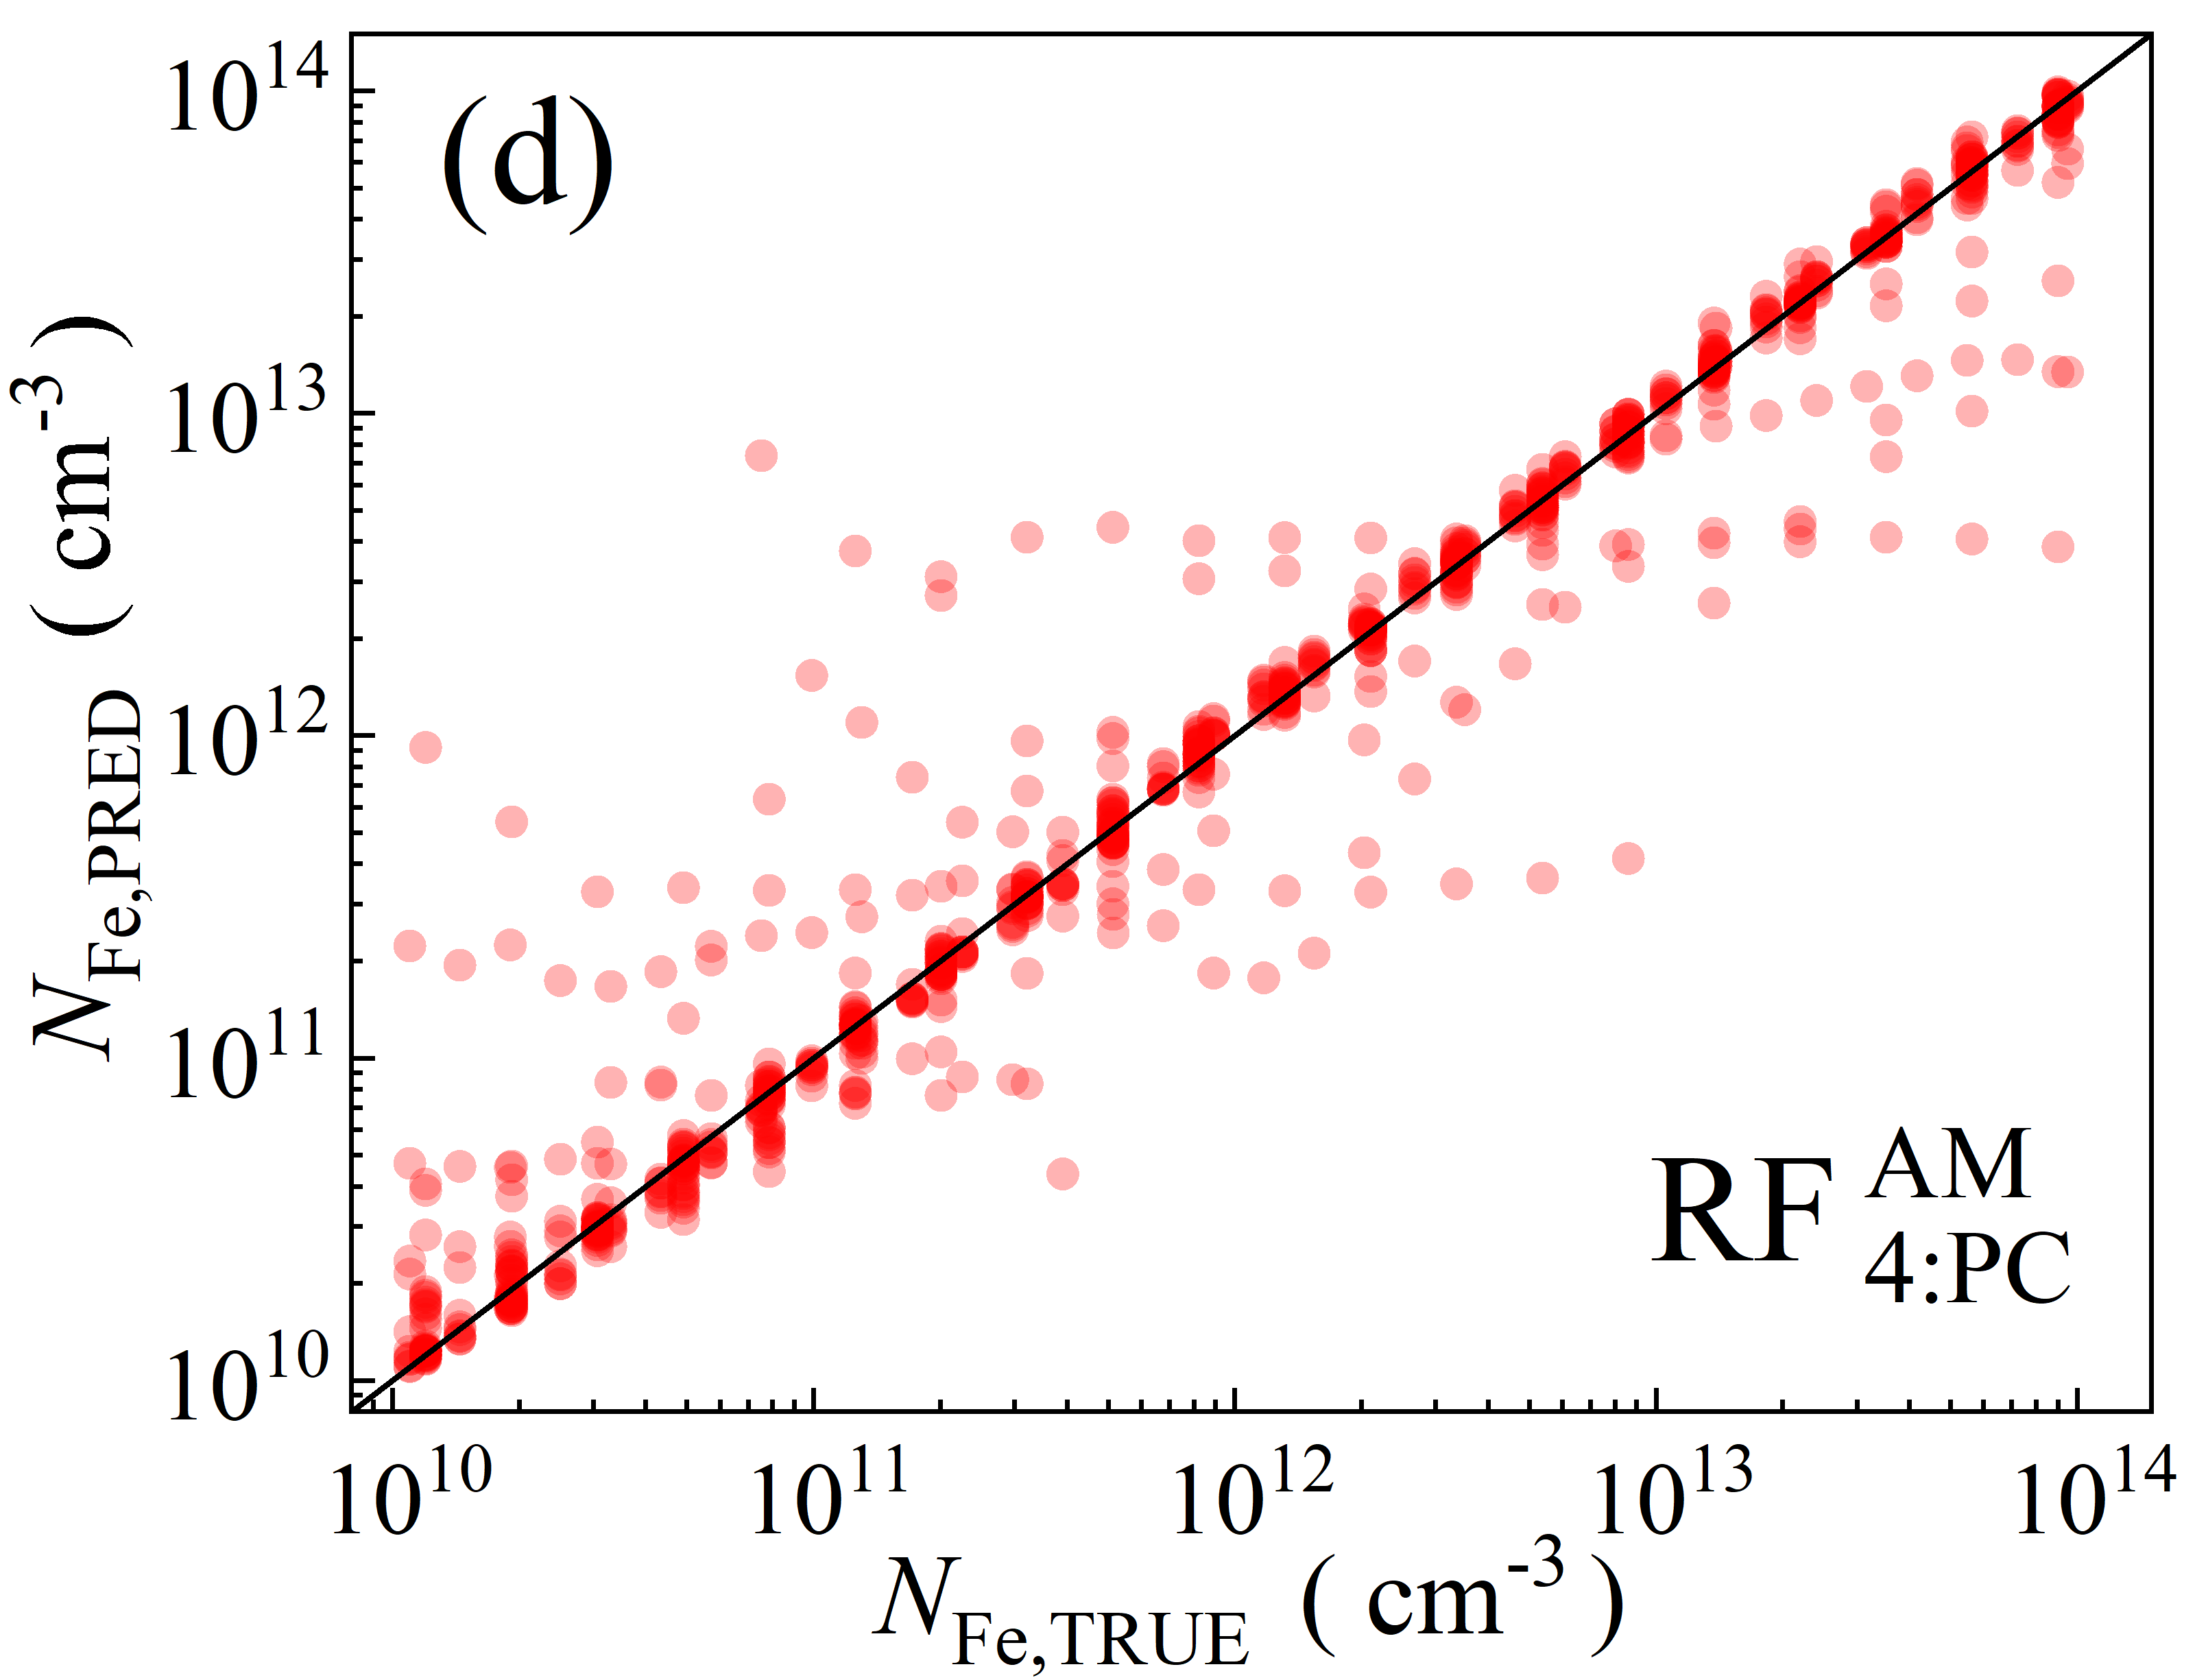
\includegraphics[width=0.24\linewidth]{Fig6d.png}
     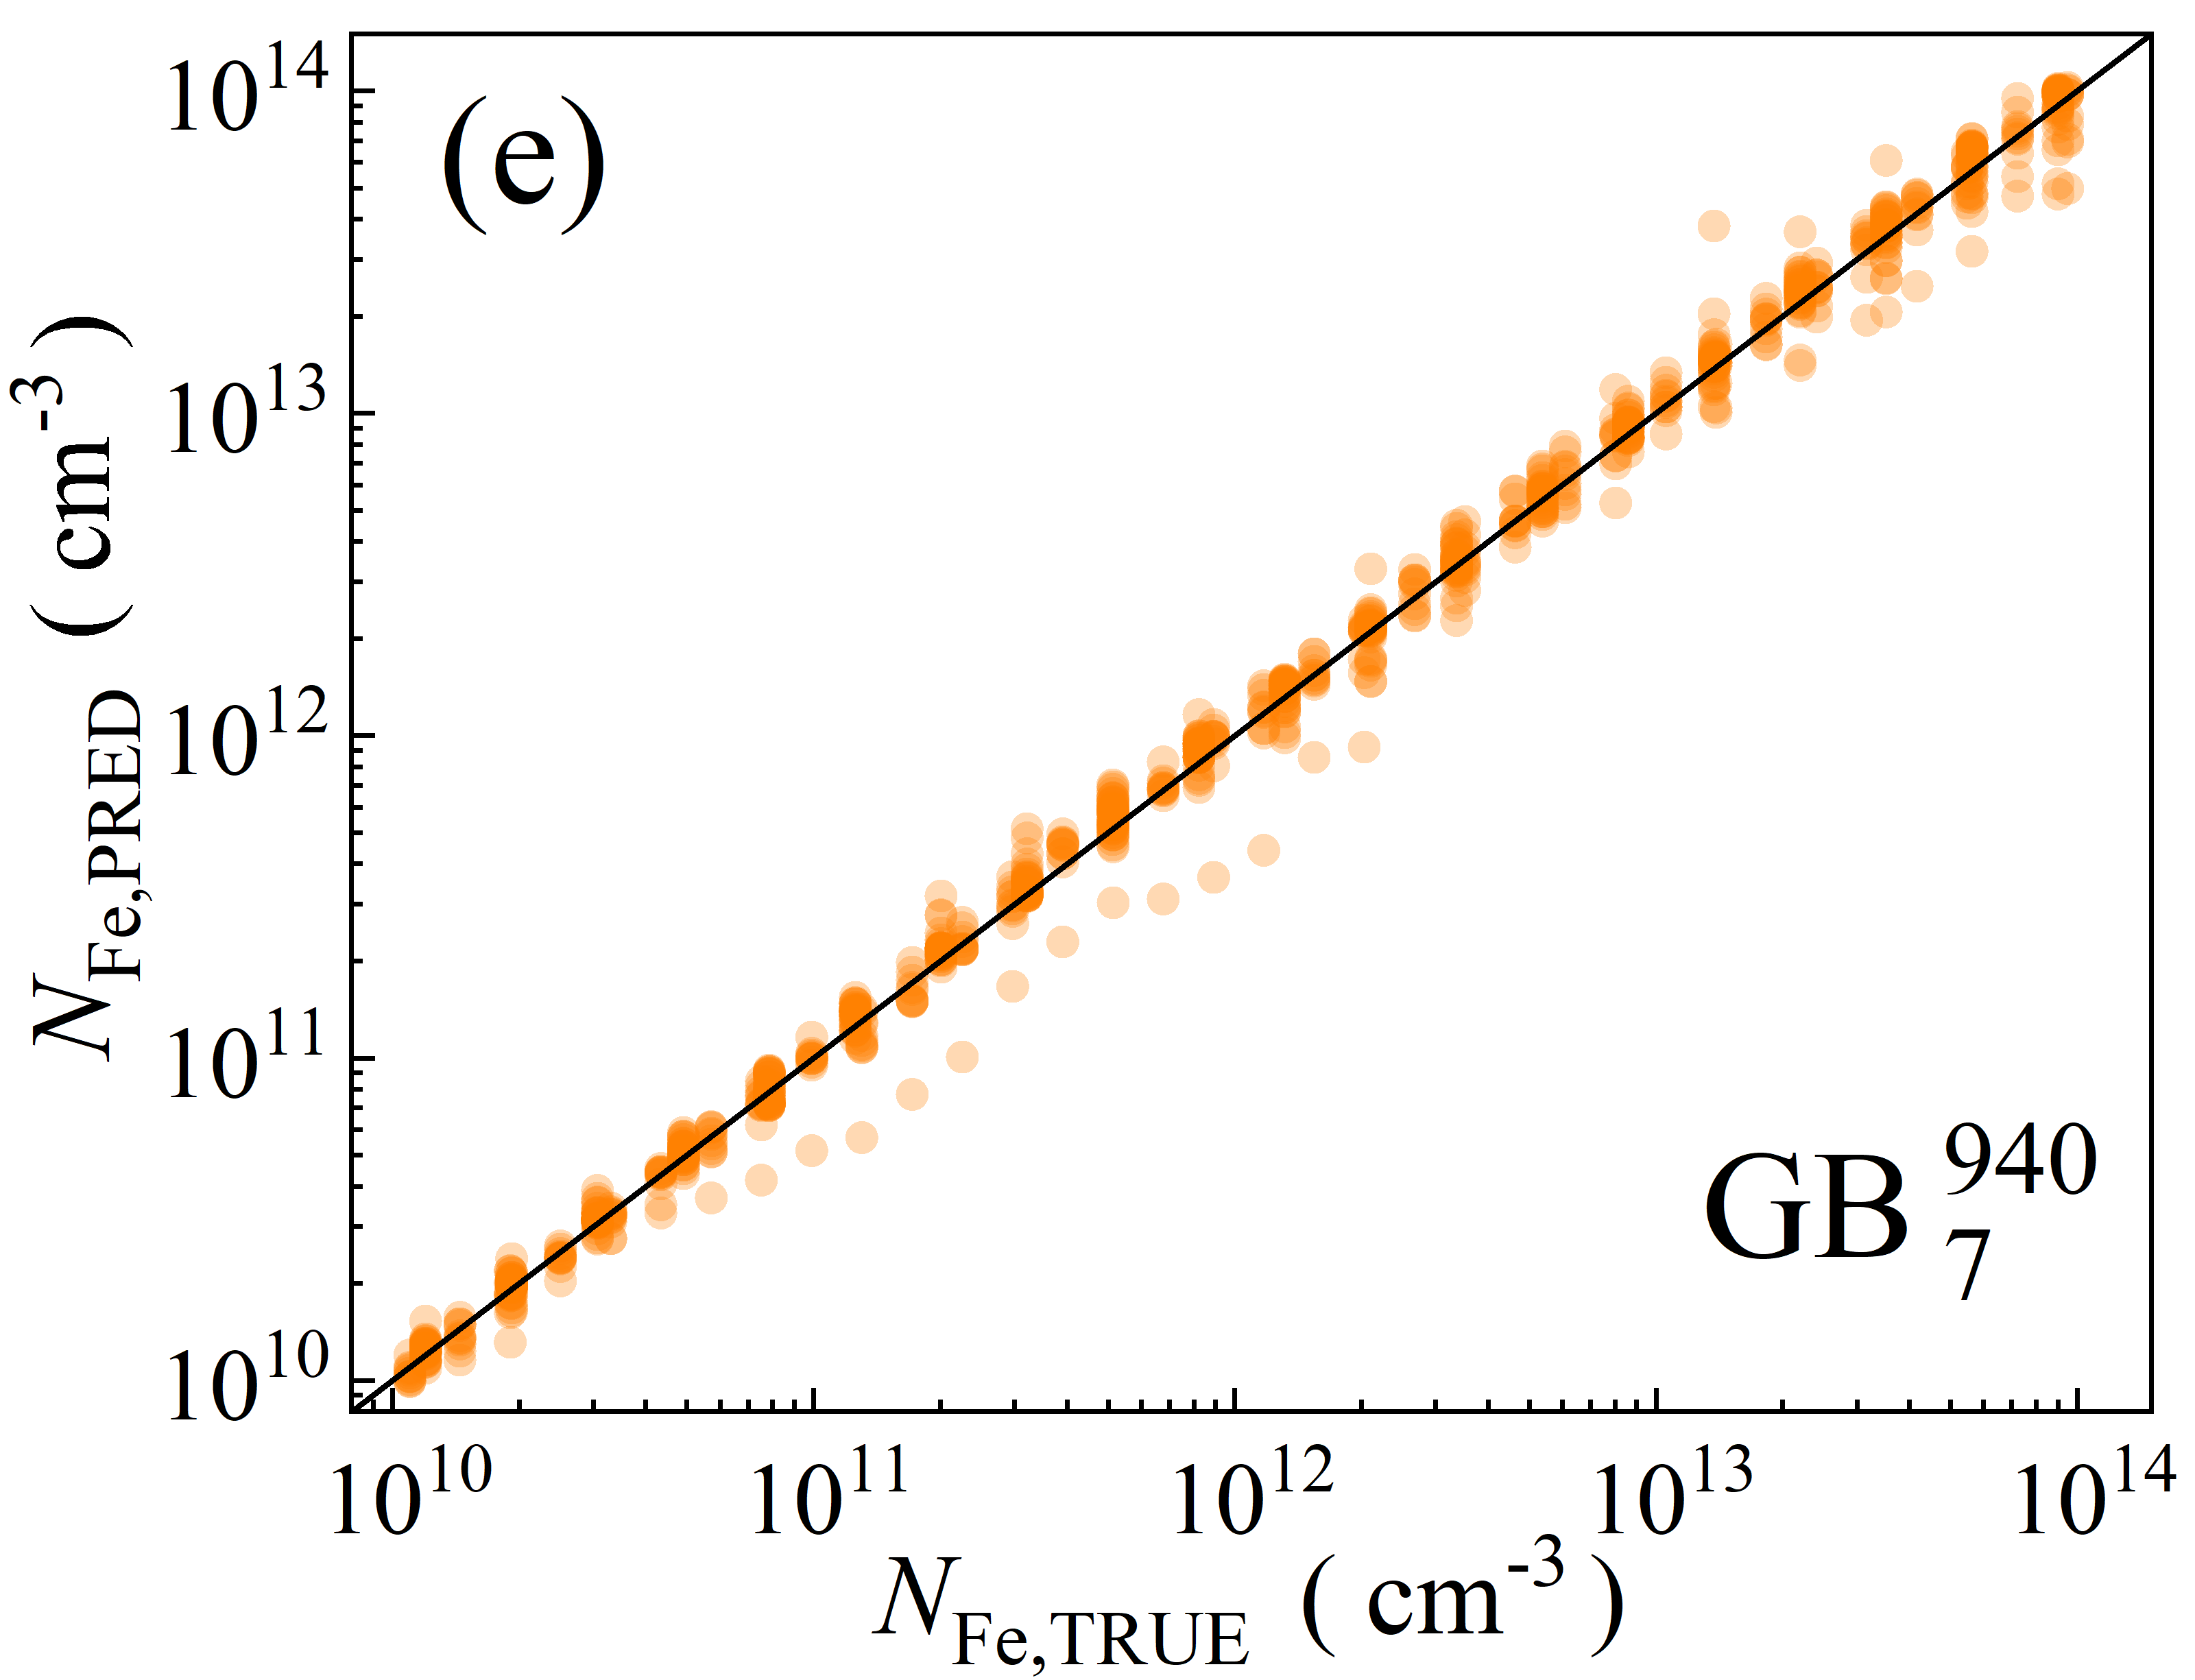
\includegraphics[width=0.24\linewidth]{Fig6e.png}
     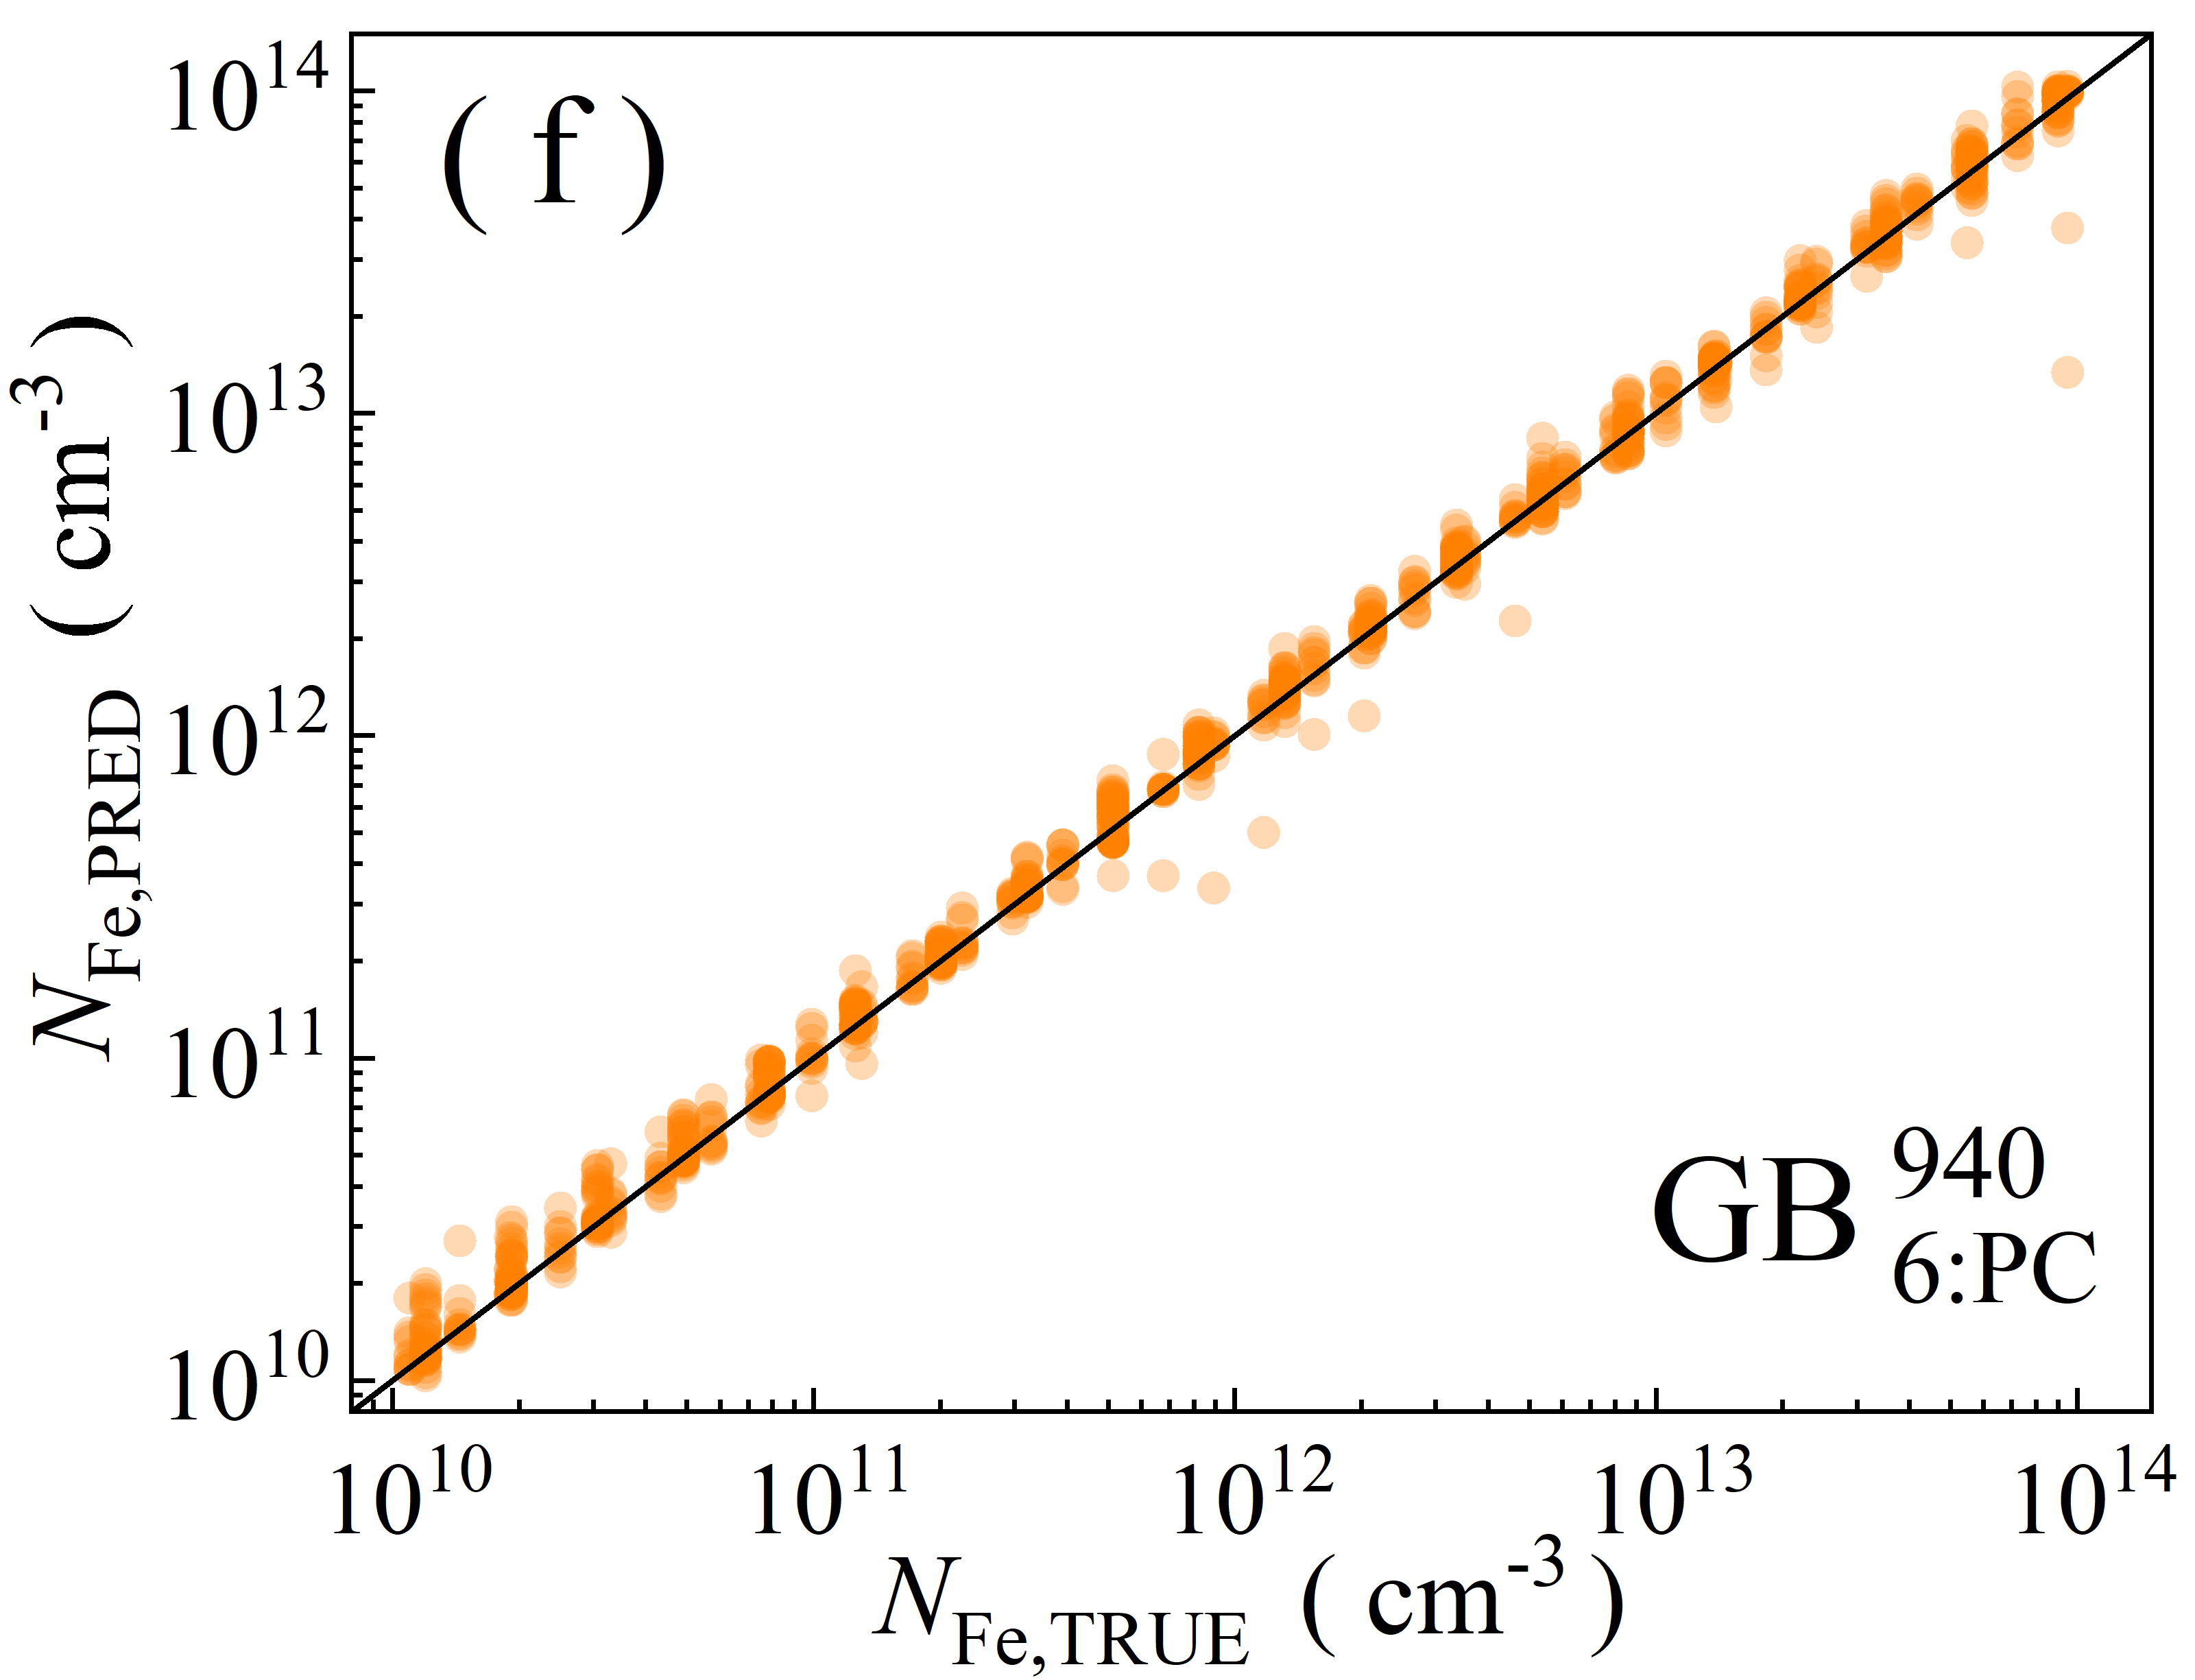
\includegraphics[width=0.24\linewidth]{Fig6f.png}
     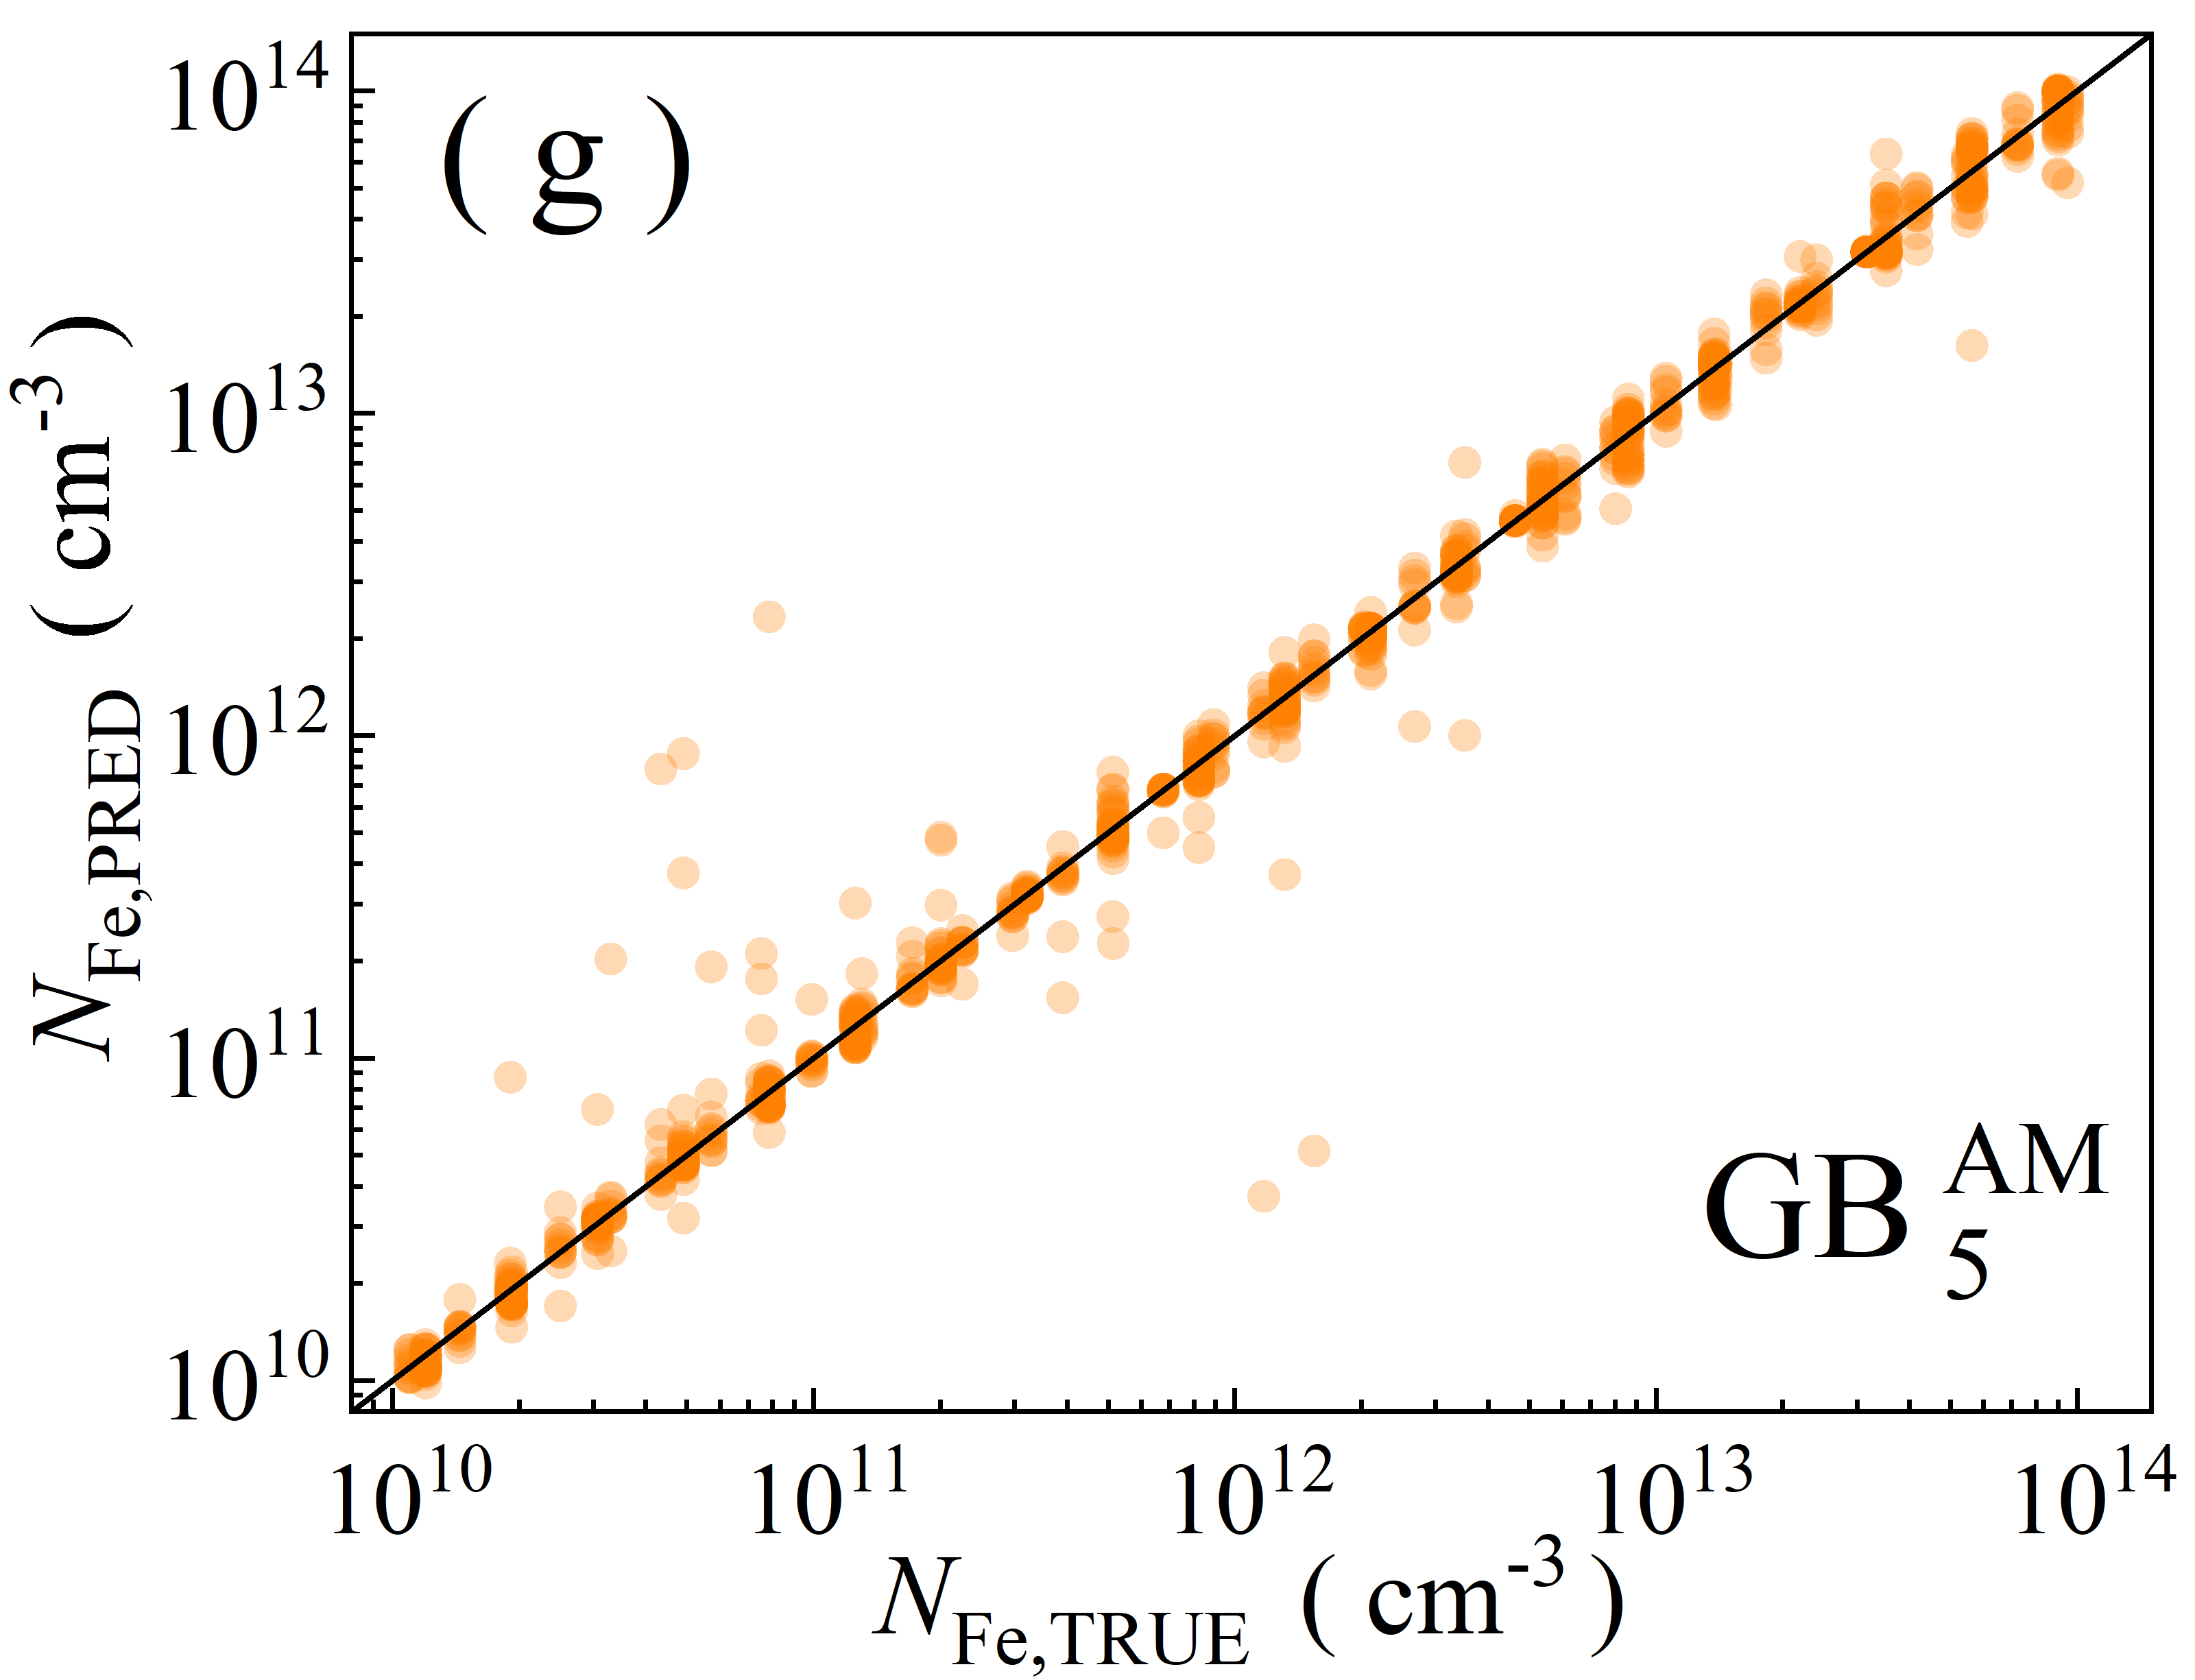
\includegraphics[width=0.24\linewidth]{Fig6g.png}
     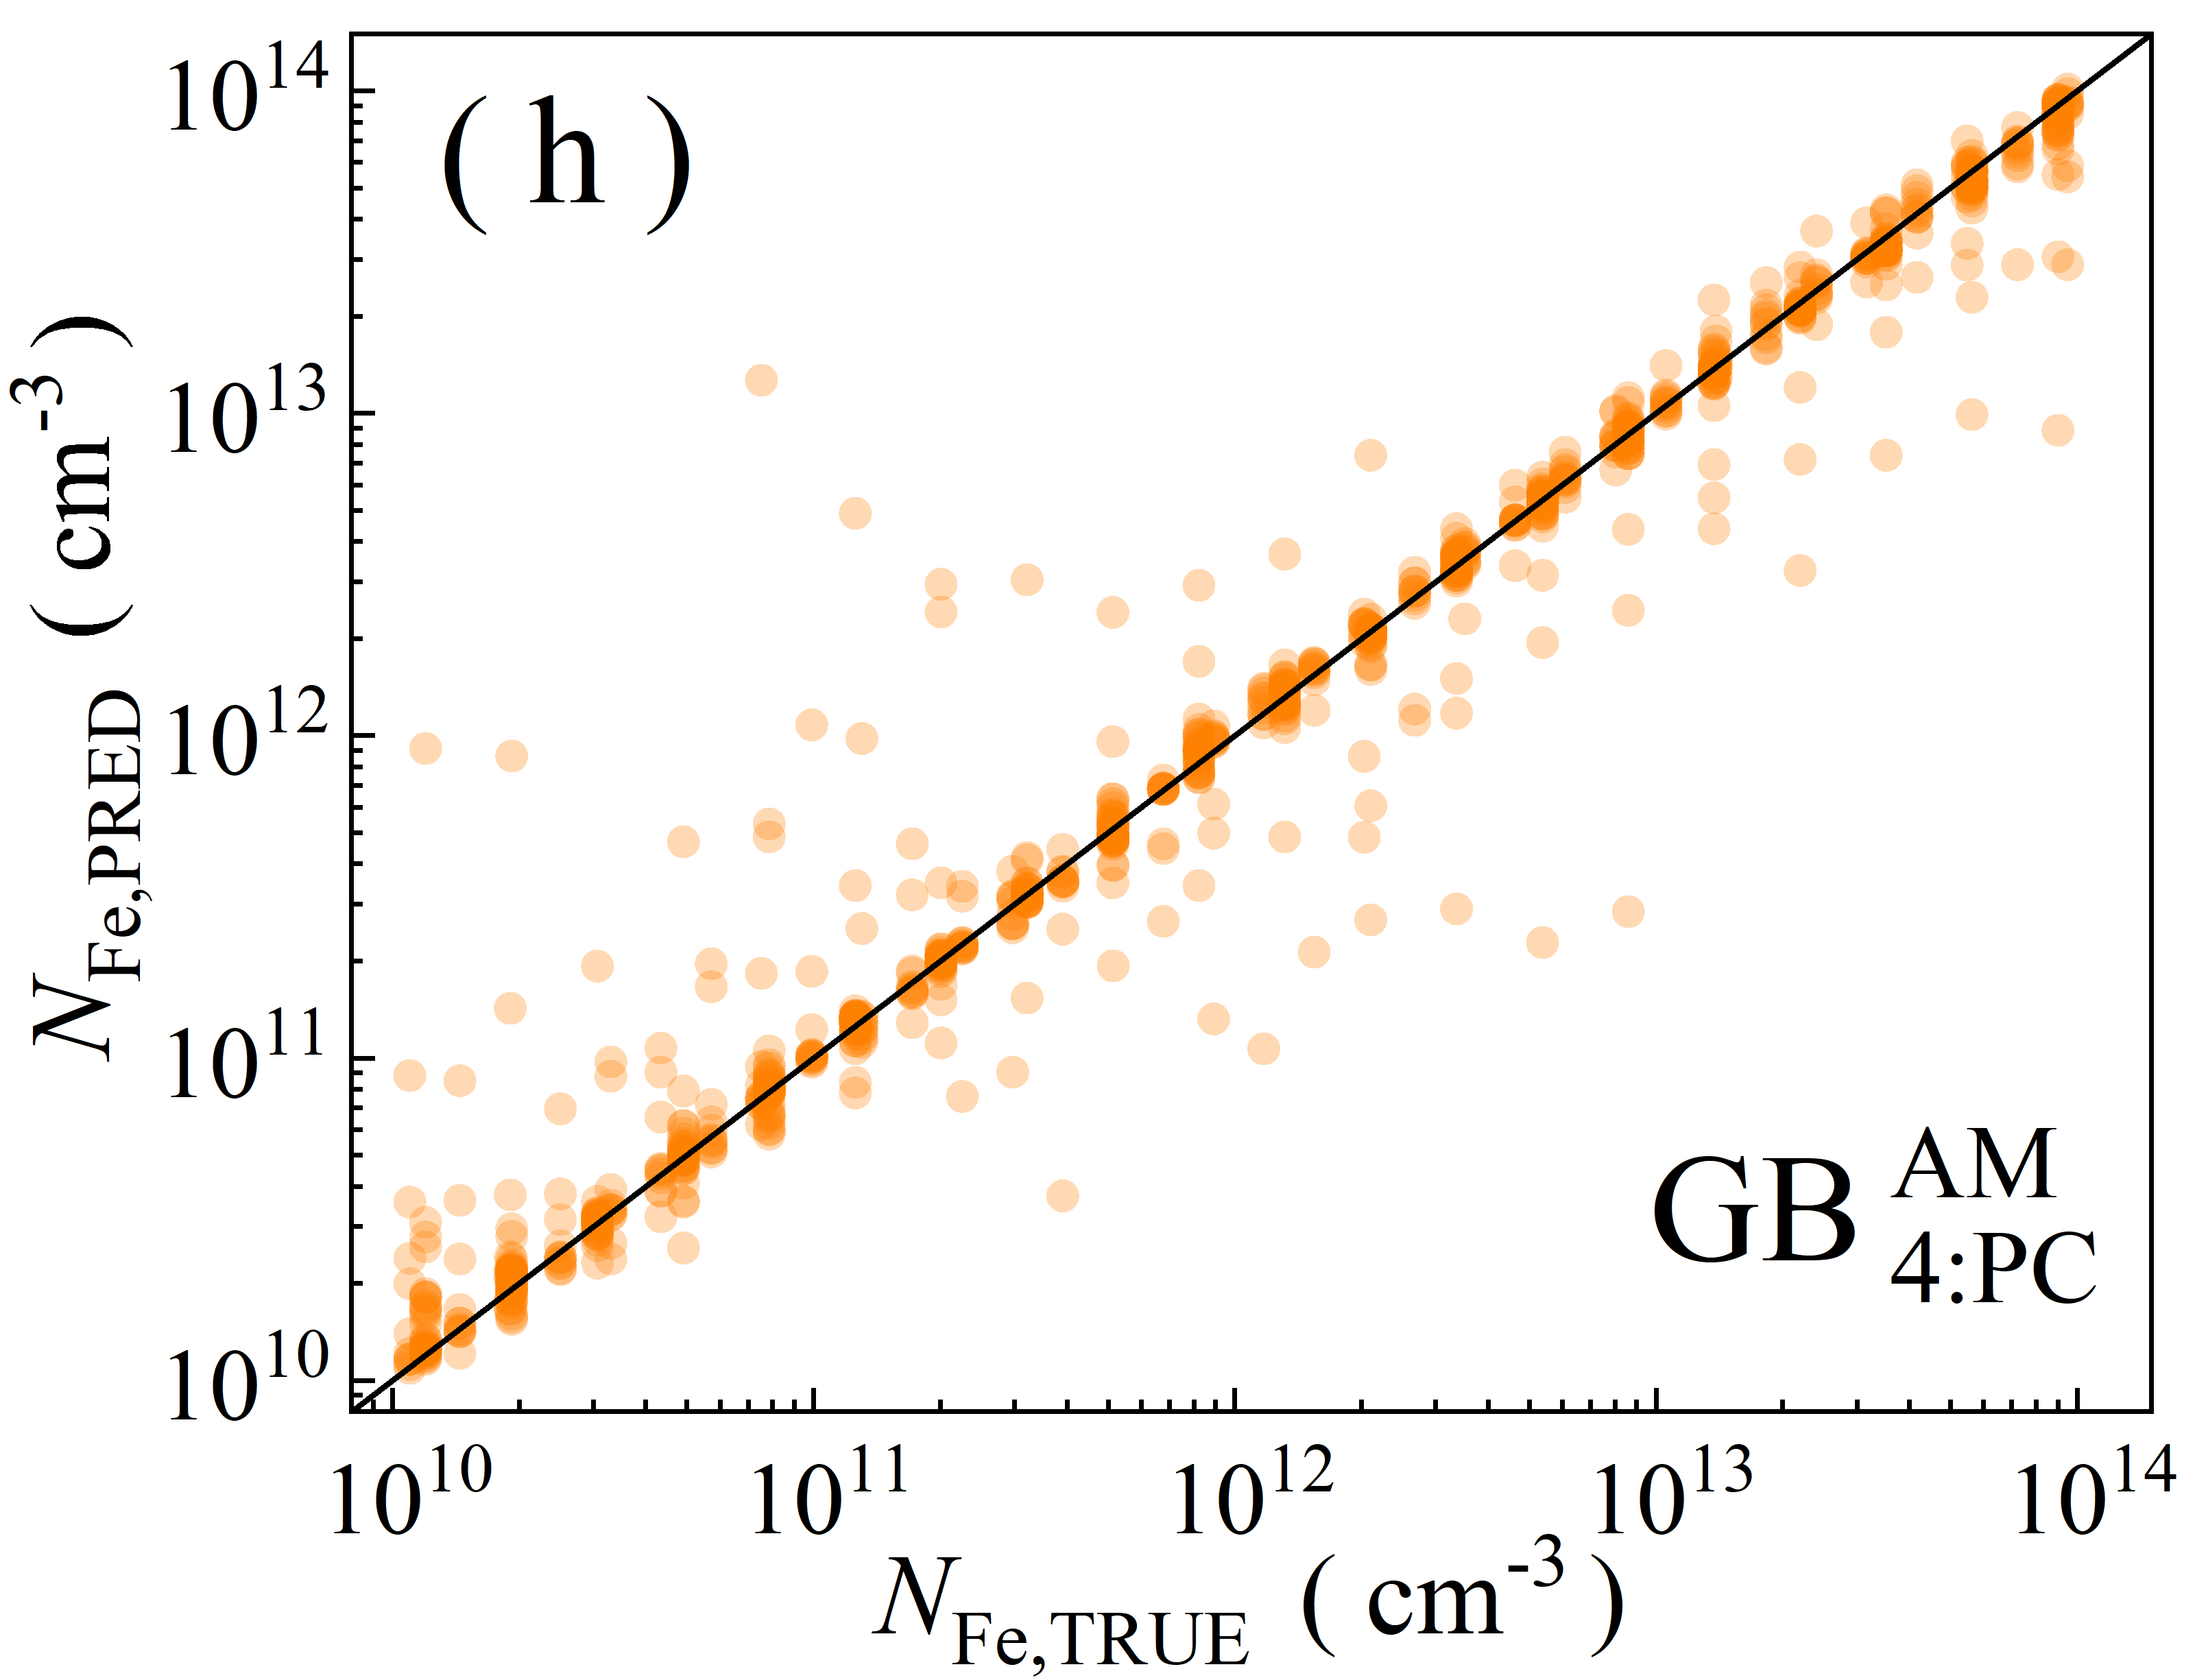
\includegraphics[width=0.24\linewidth]{Fig6h.png}
     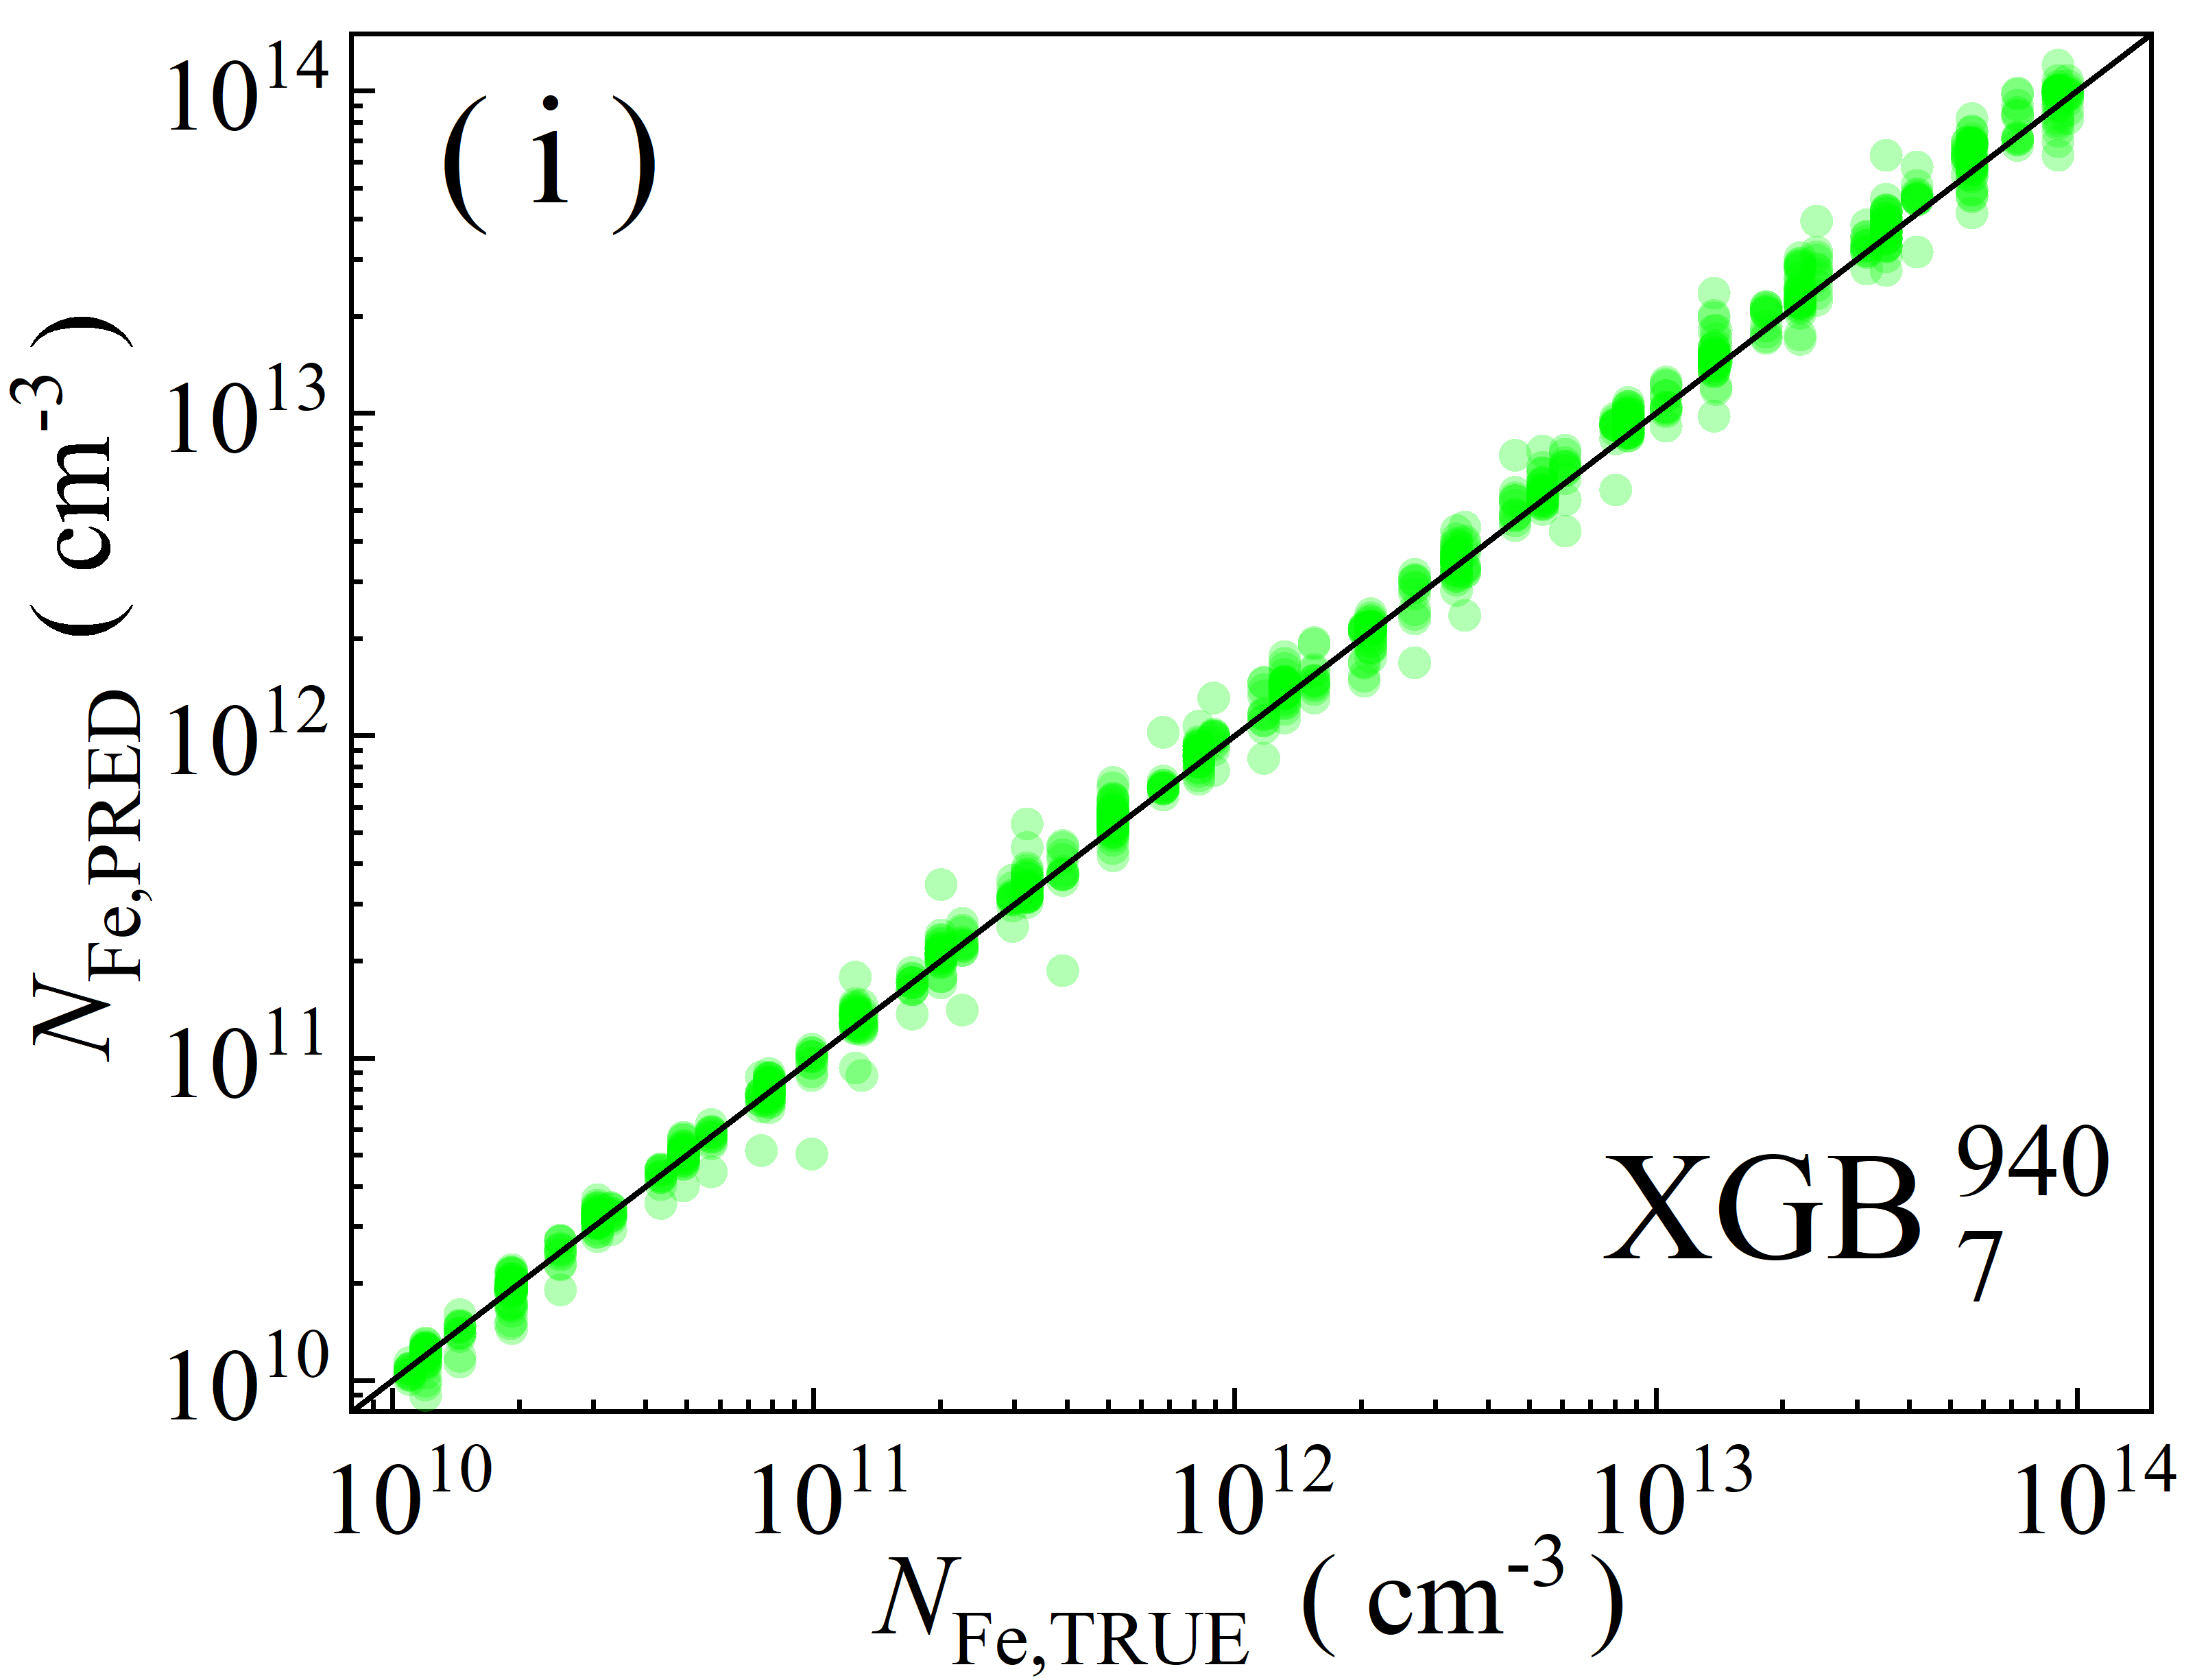
\includegraphics[width=0.24\linewidth]{Fig6i.png}
     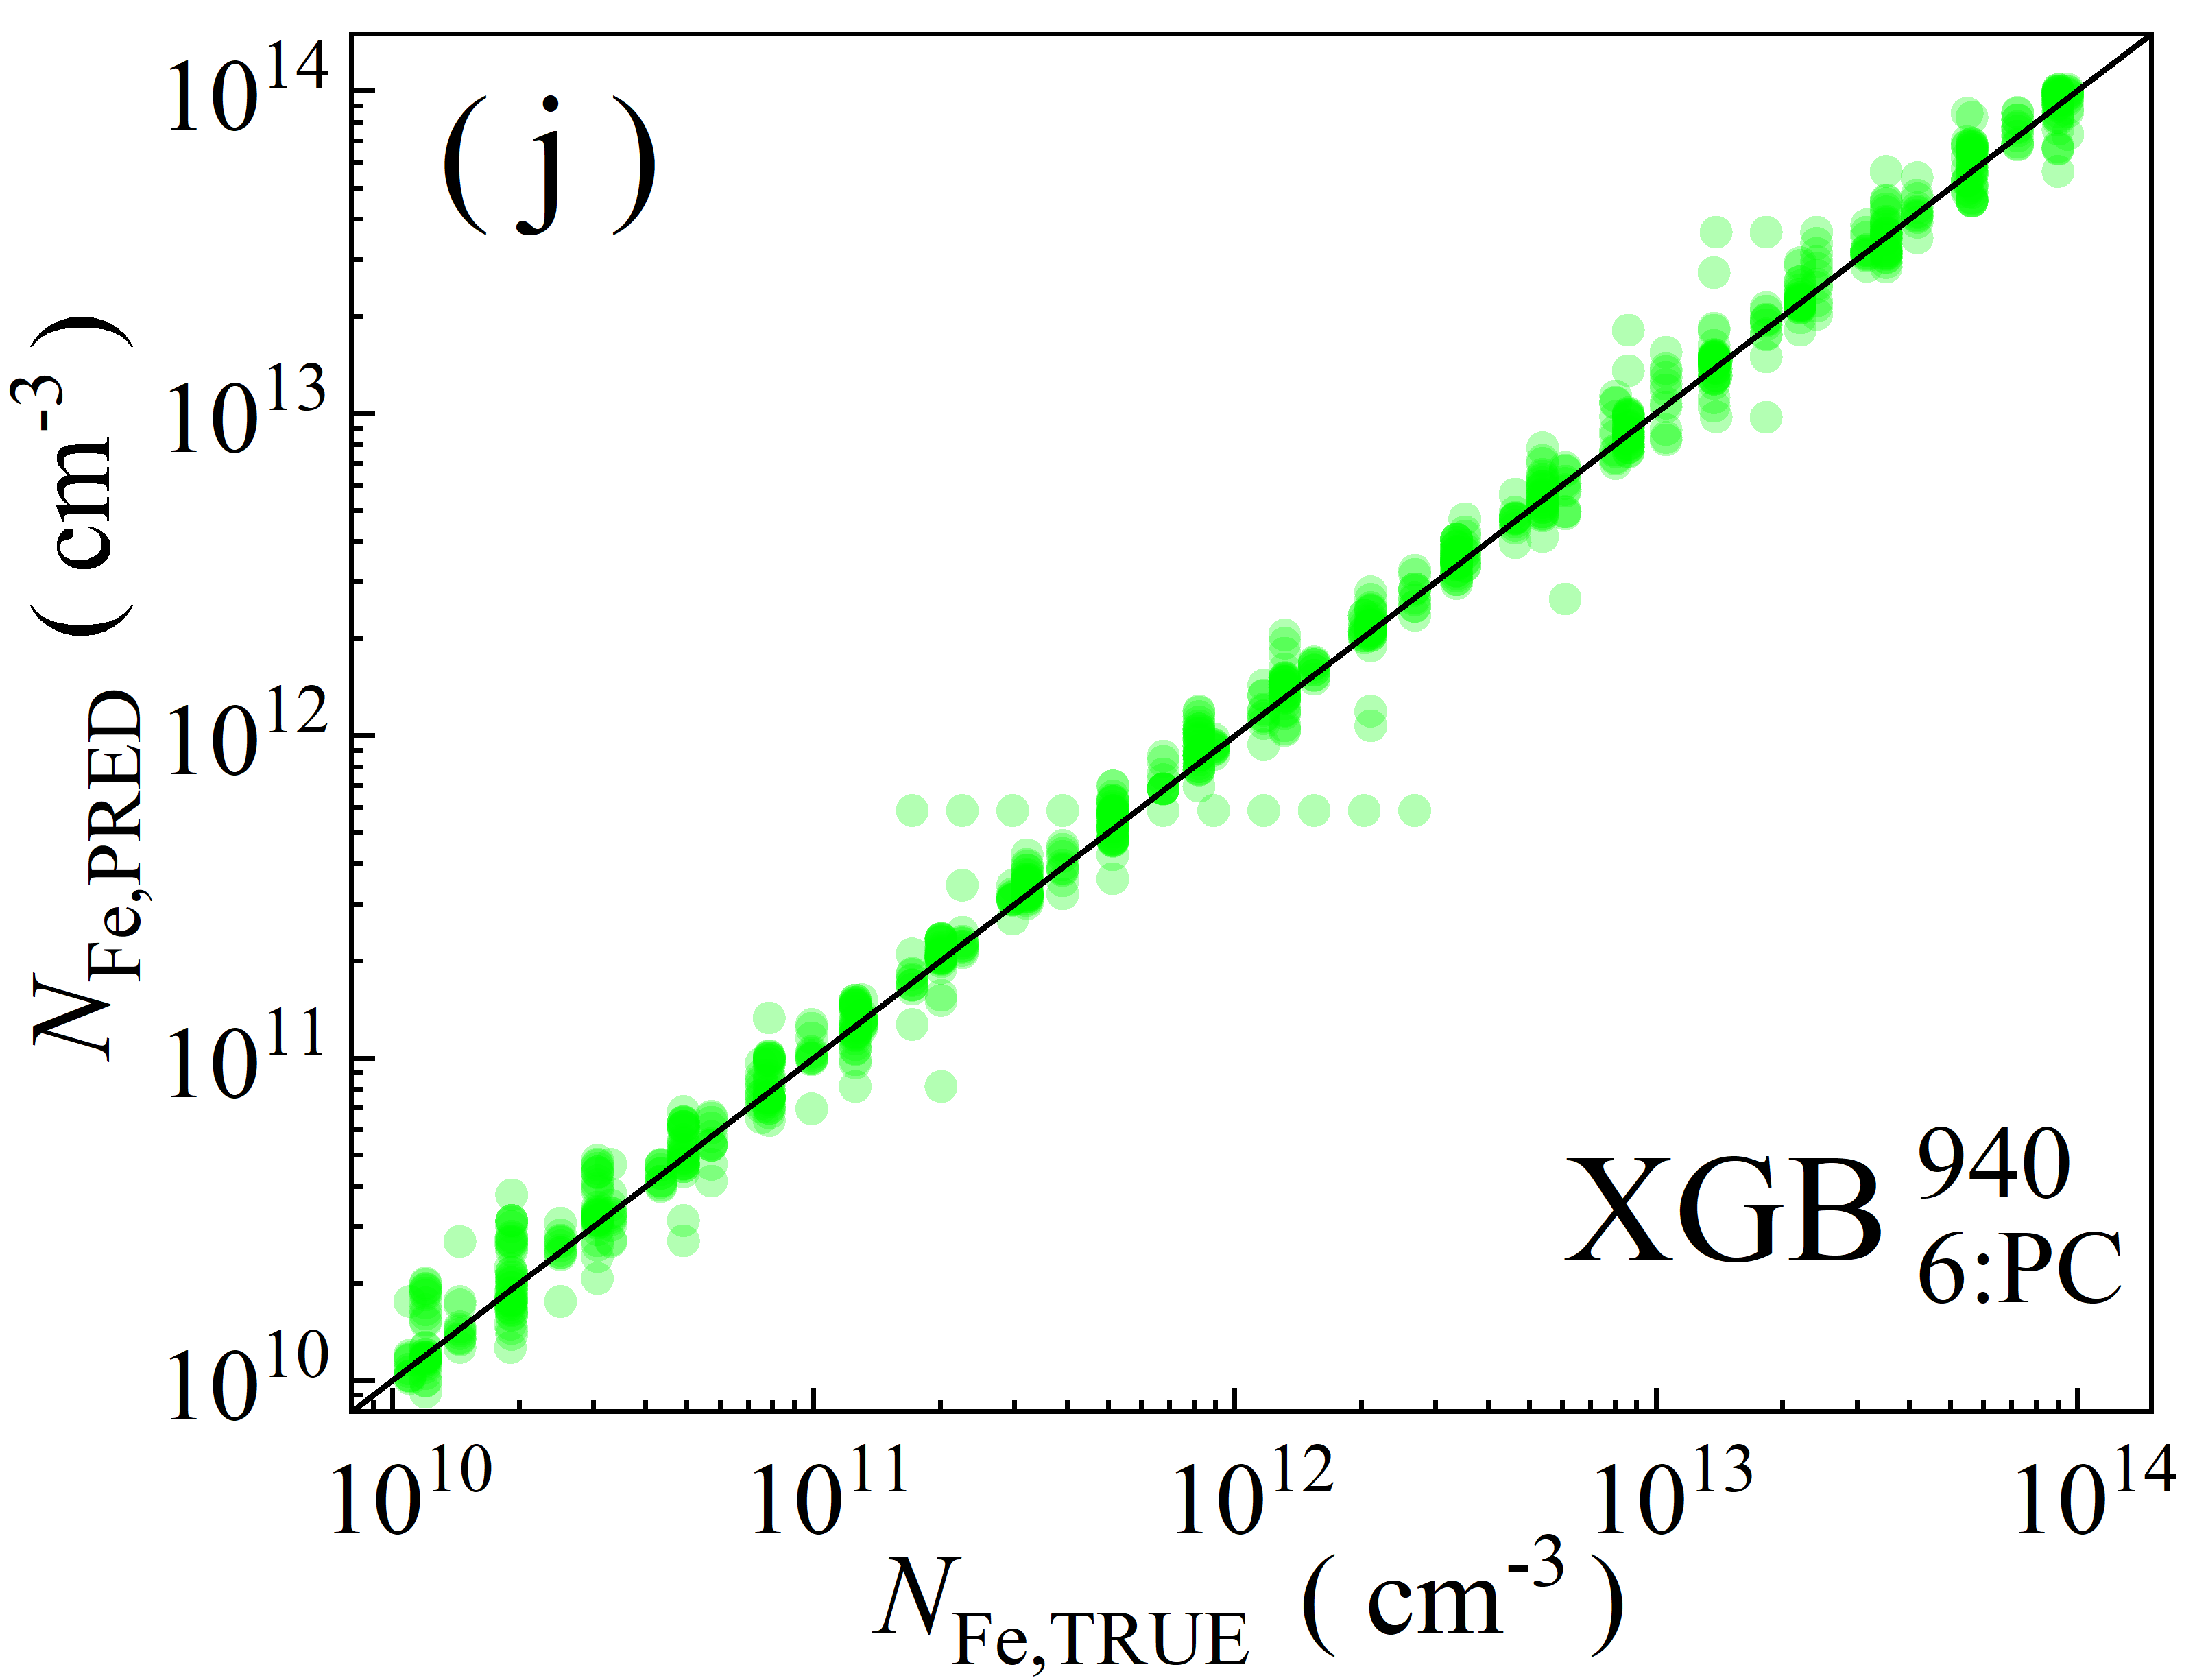
\includegraphics[width=0.24\linewidth]{Fig6j.png}
     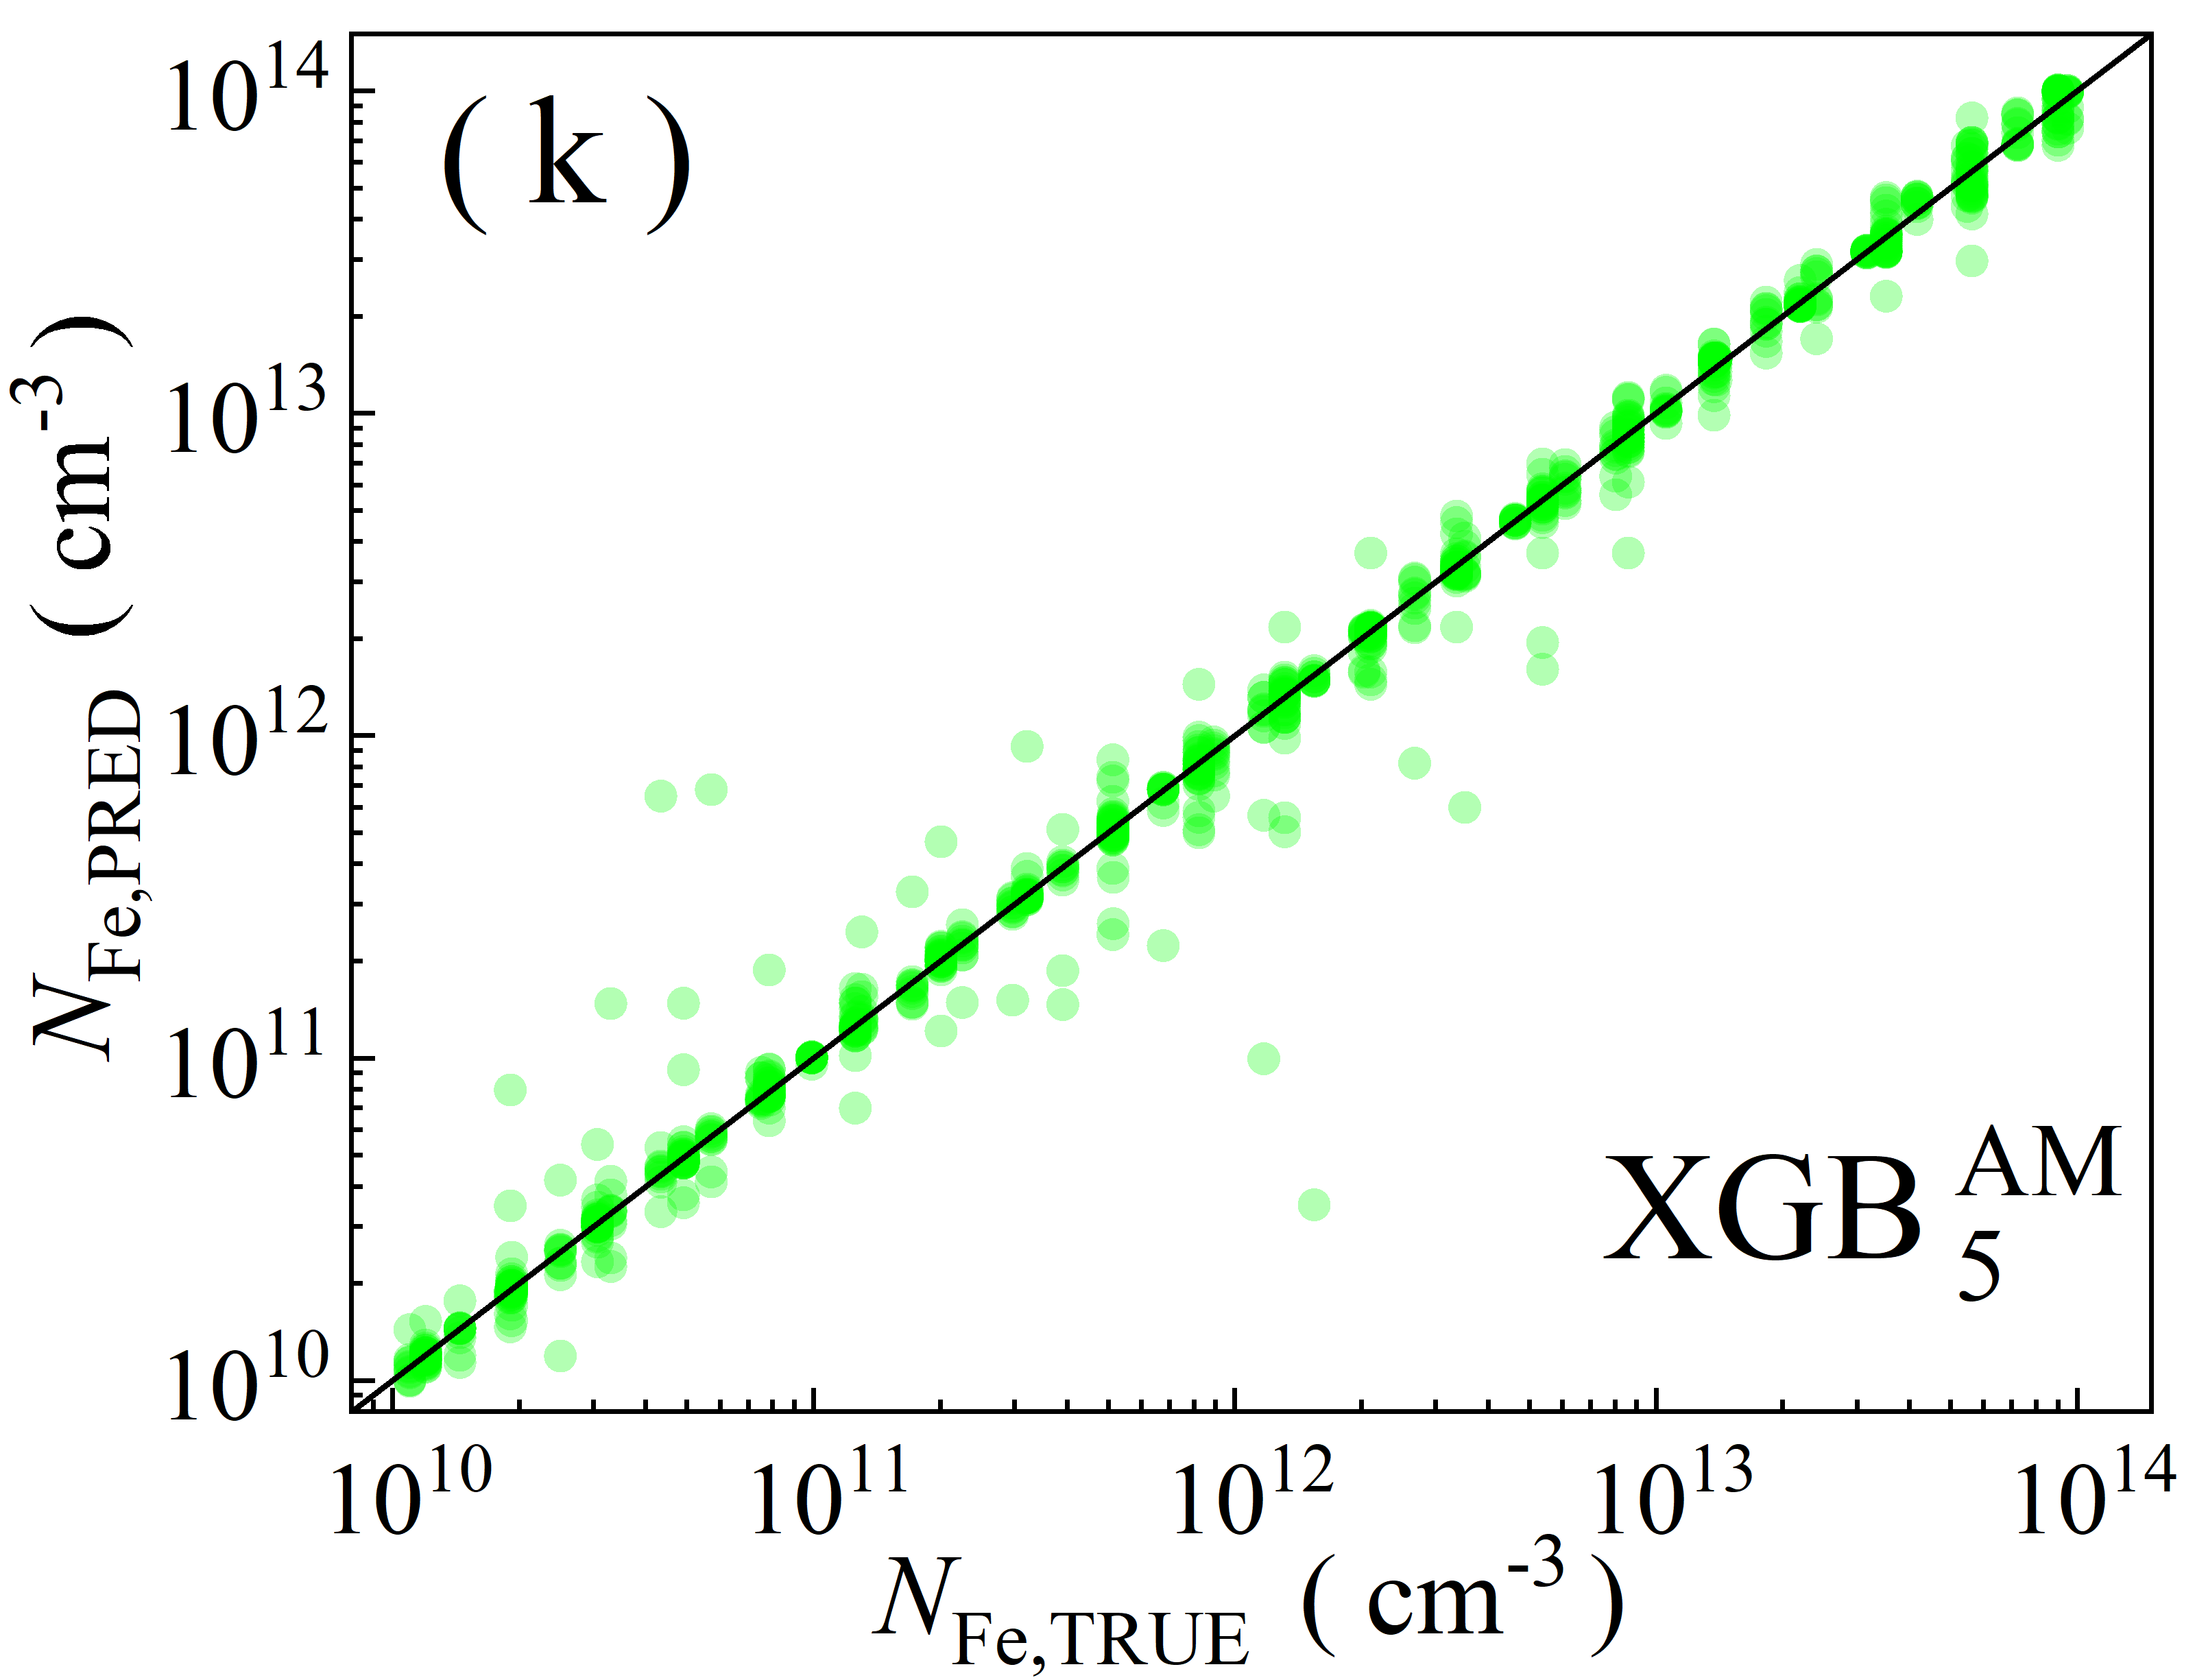
\includegraphics[width=0.24\linewidth]{Fig6k.png}
     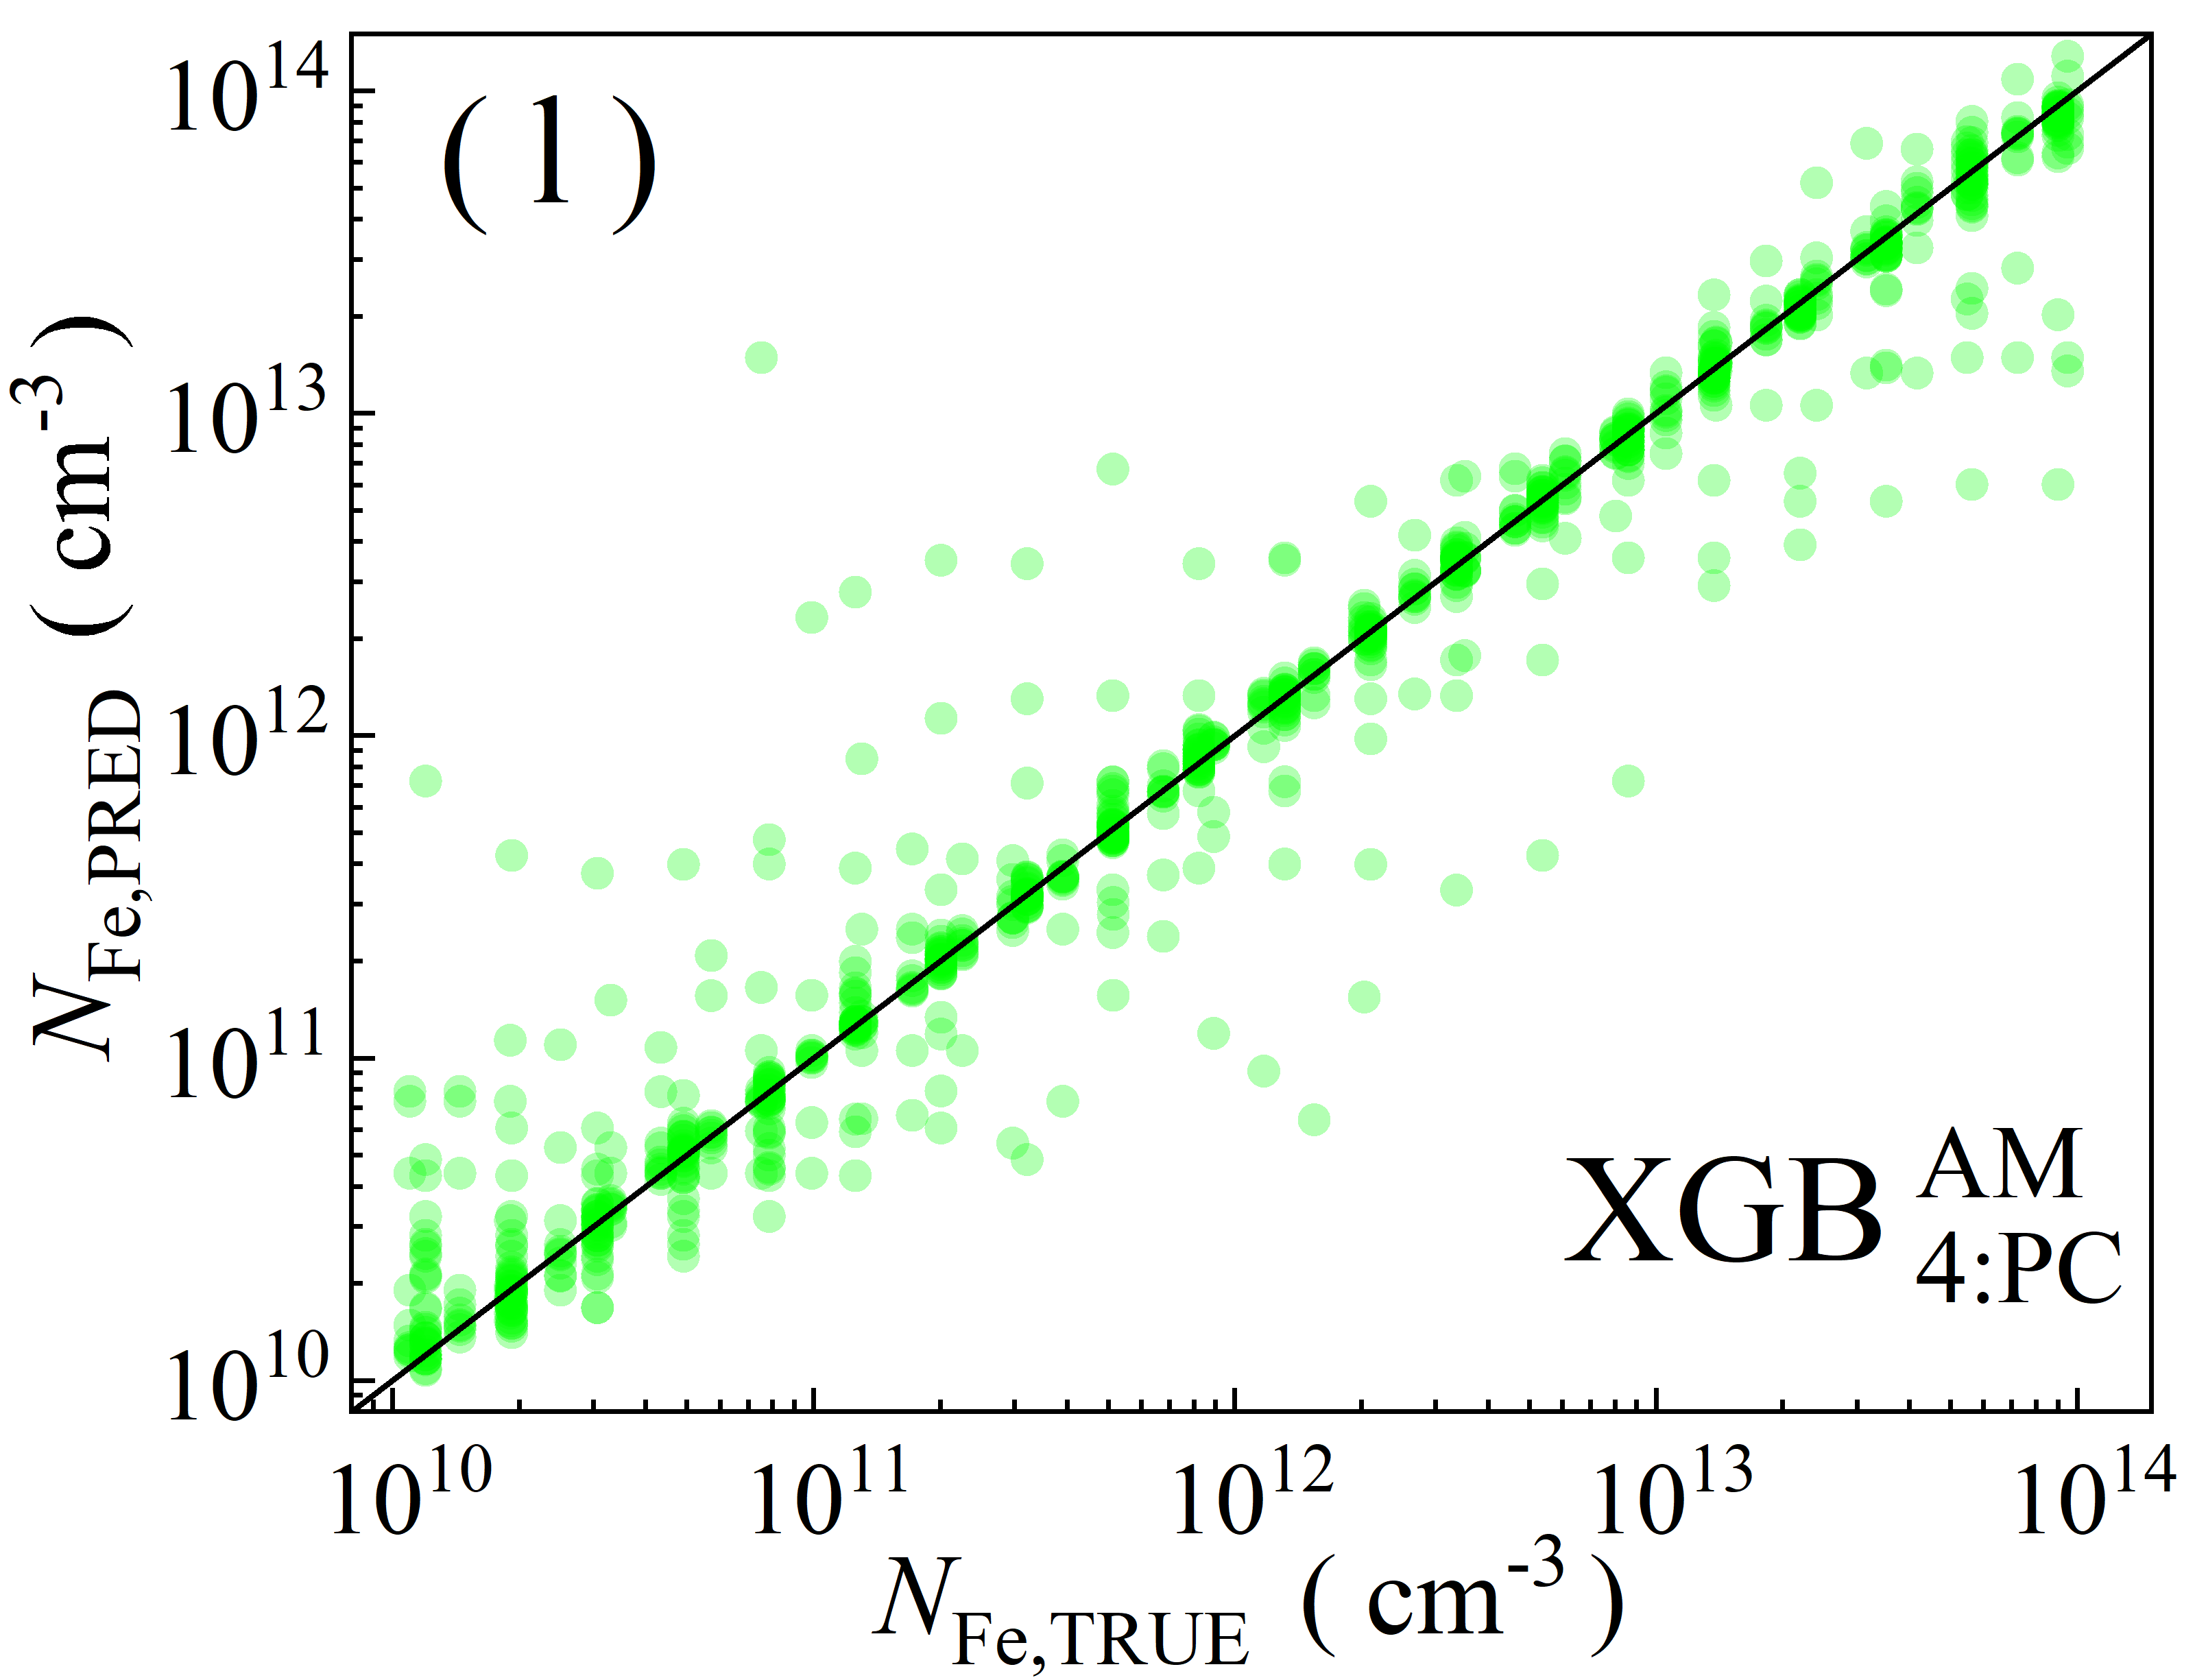
\includegraphics[width=0.24\linewidth]{Fig6l.png}
     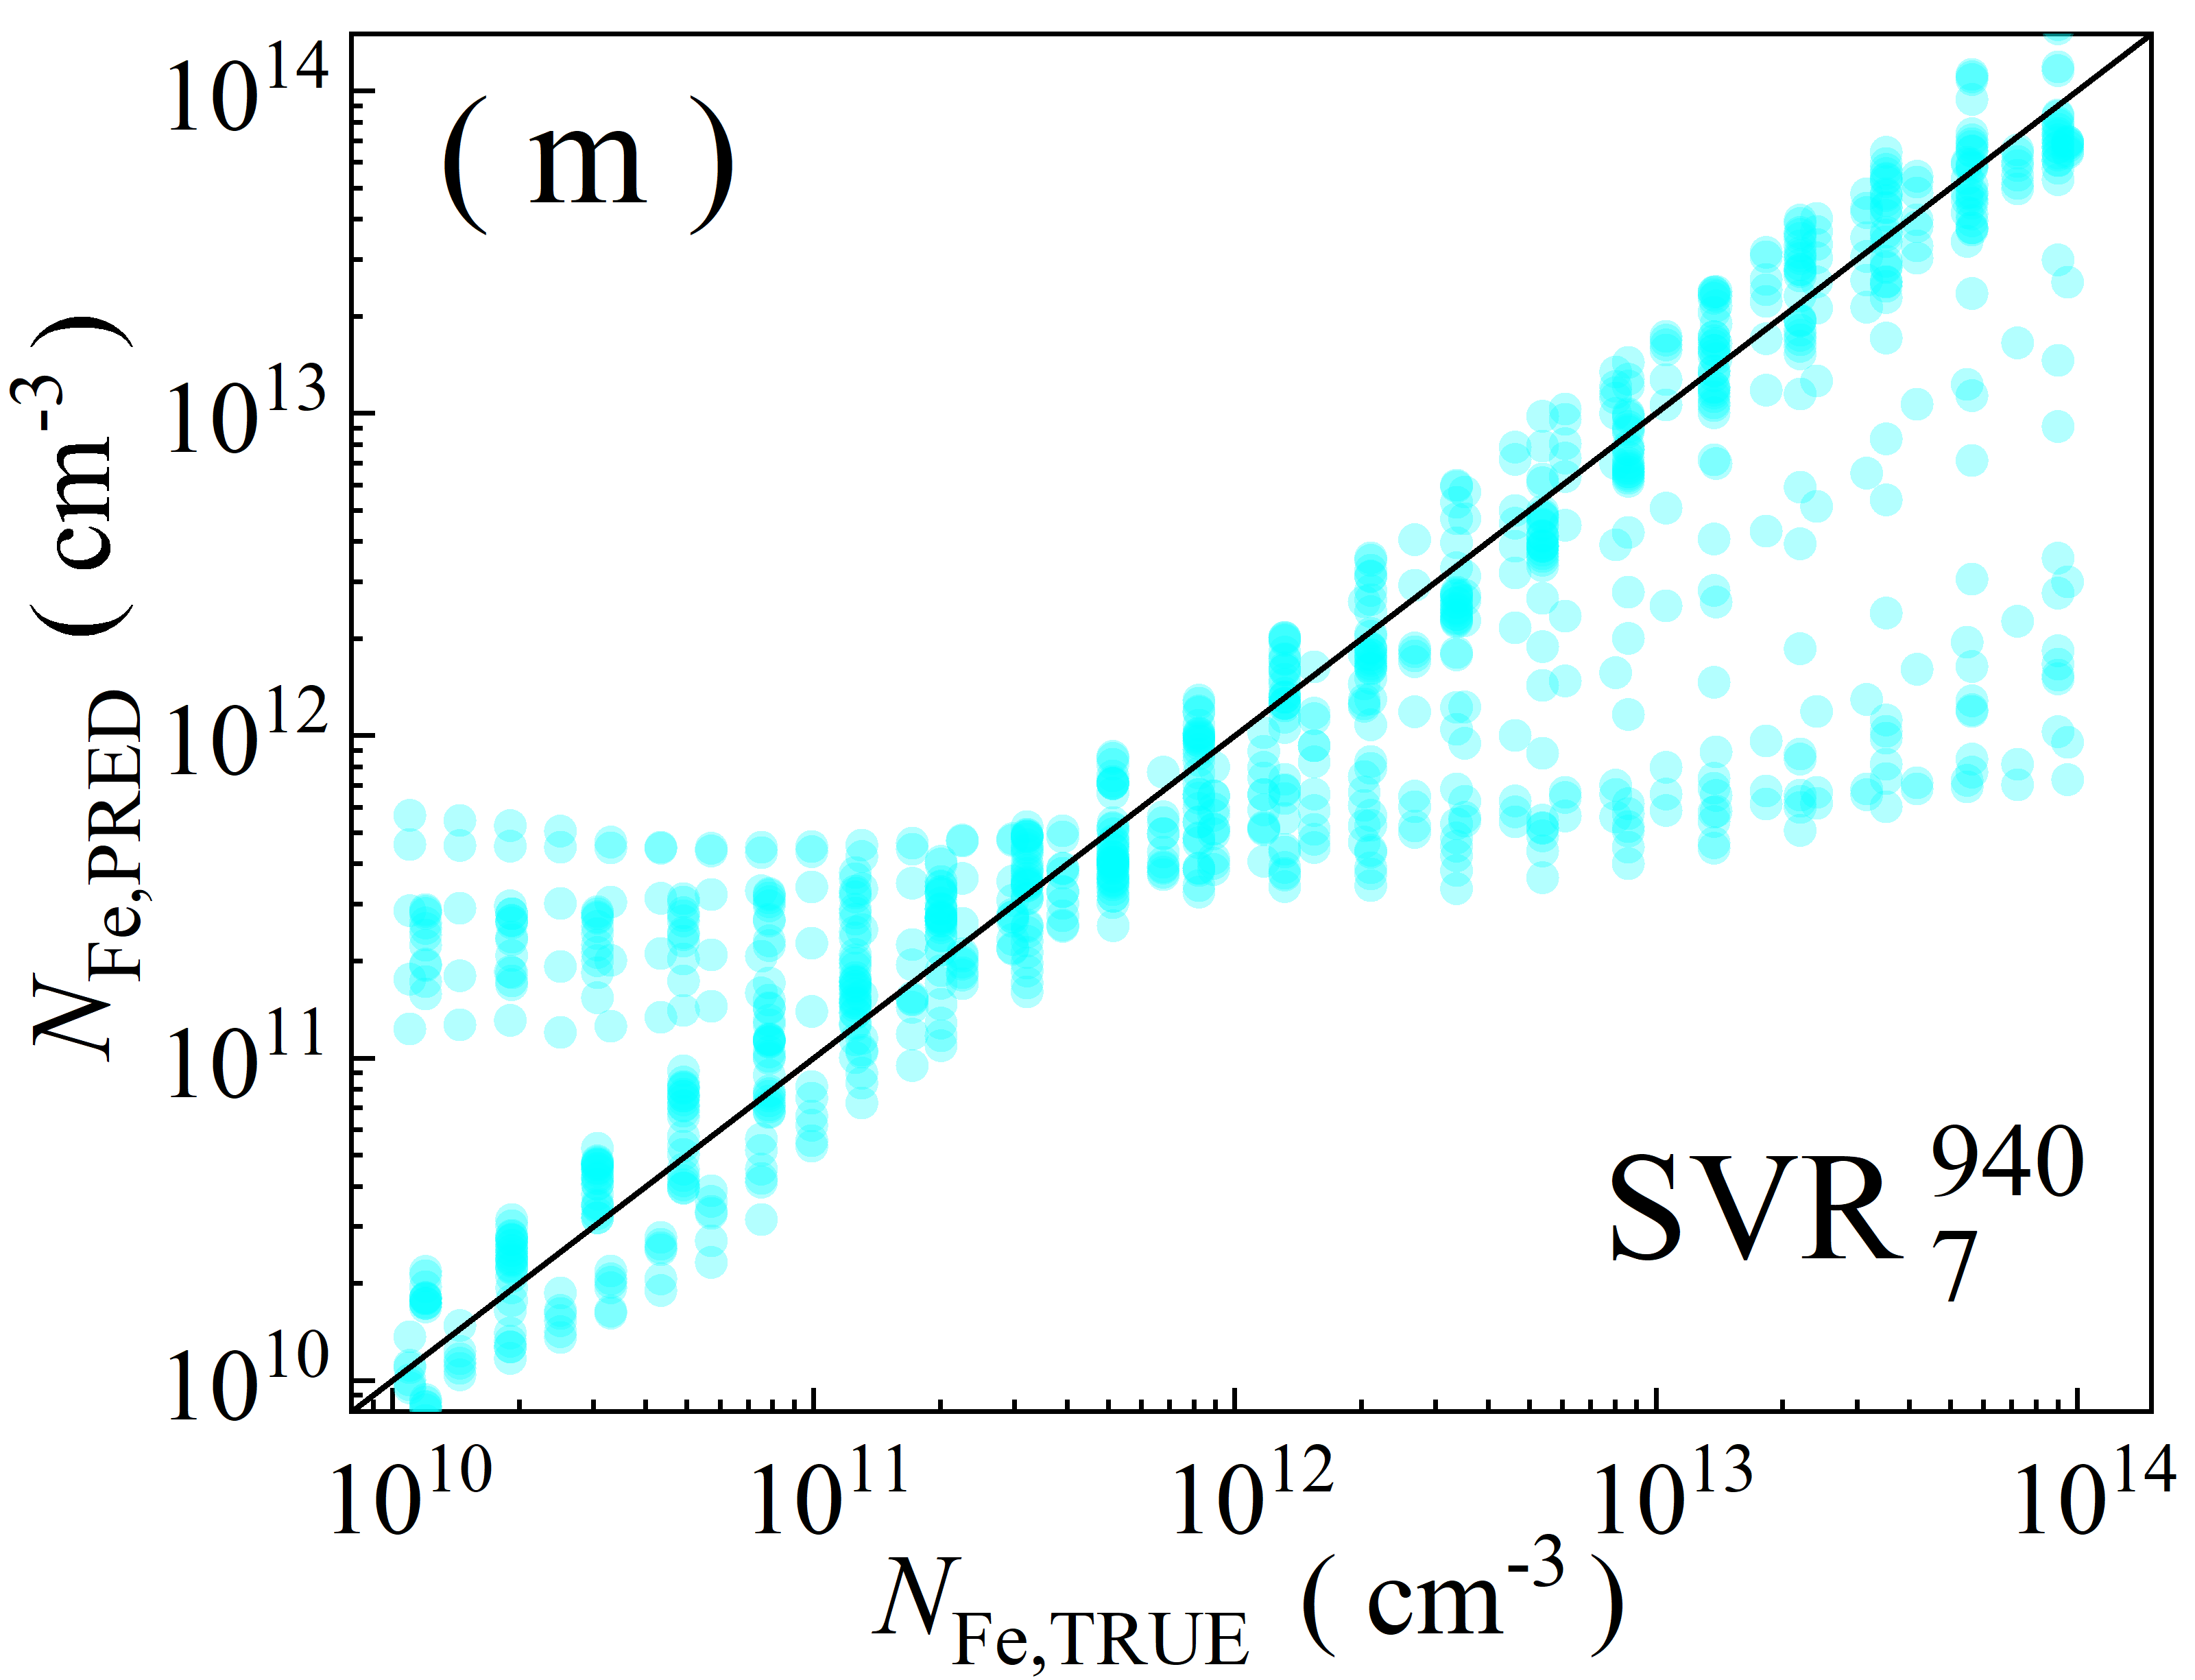
\includegraphics[width=0.24\linewidth]{Fig6m.png}
     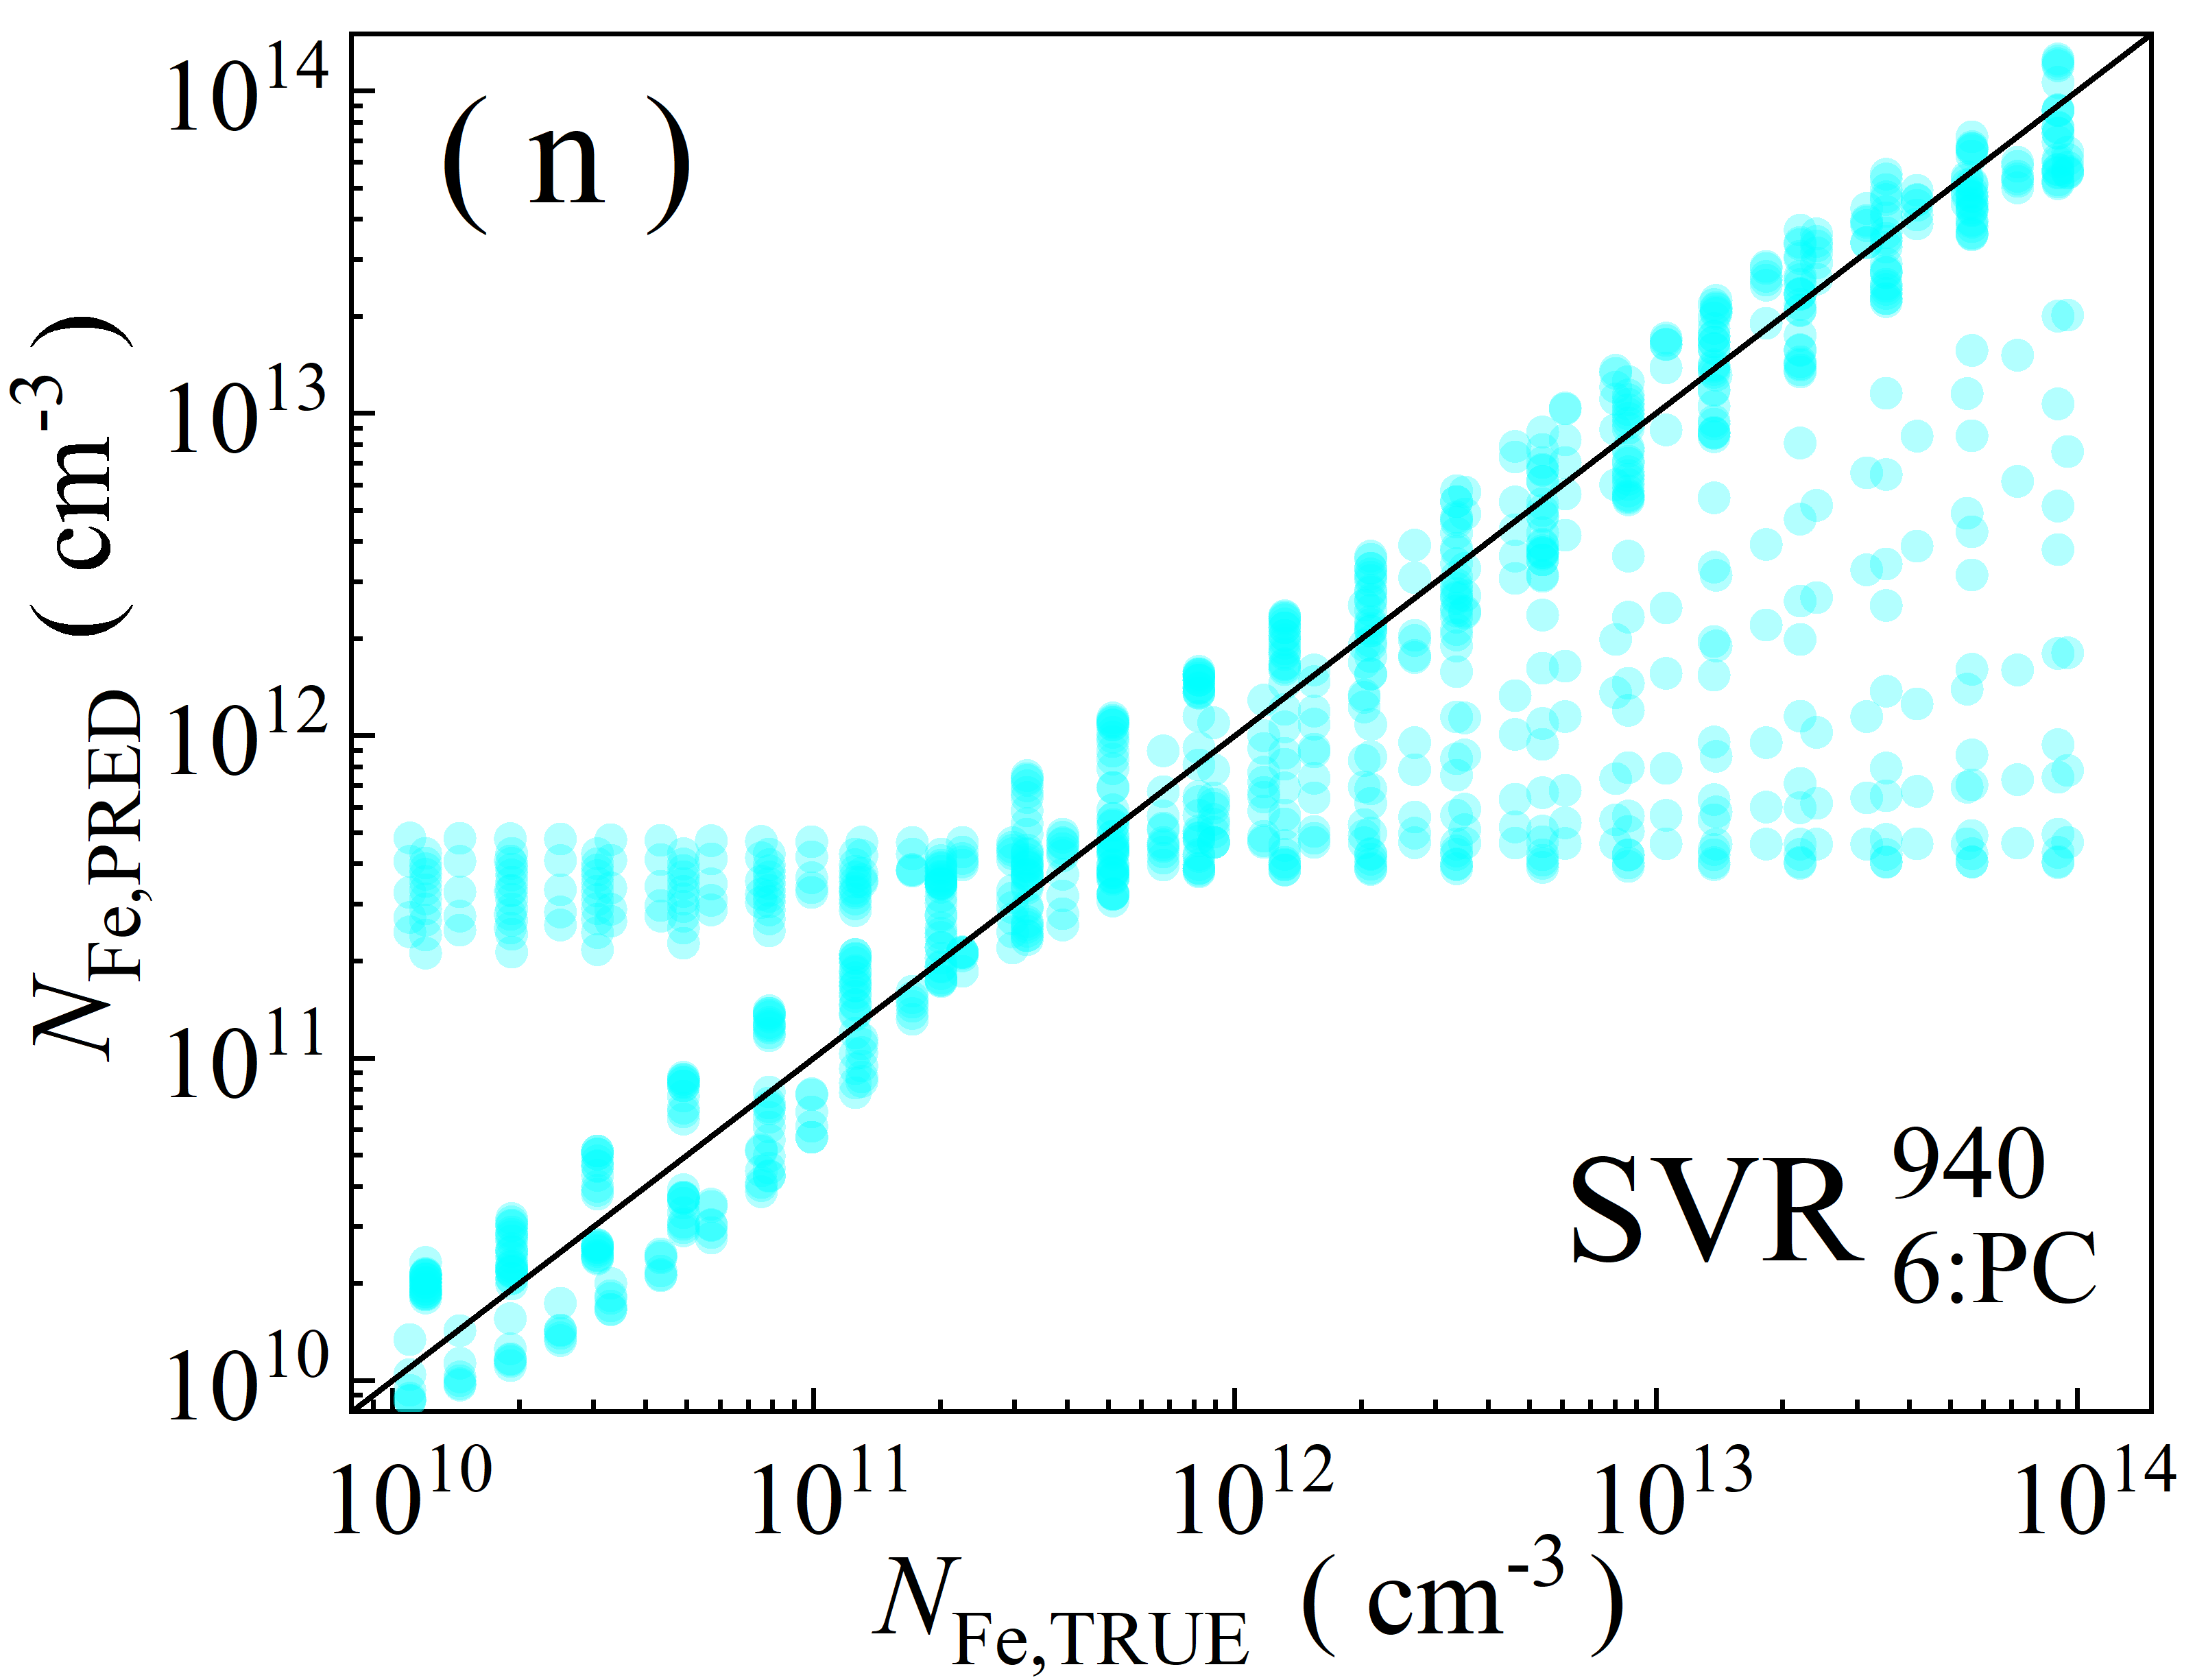
\includegraphics[width=0.24\linewidth]{Fig6n.png}
     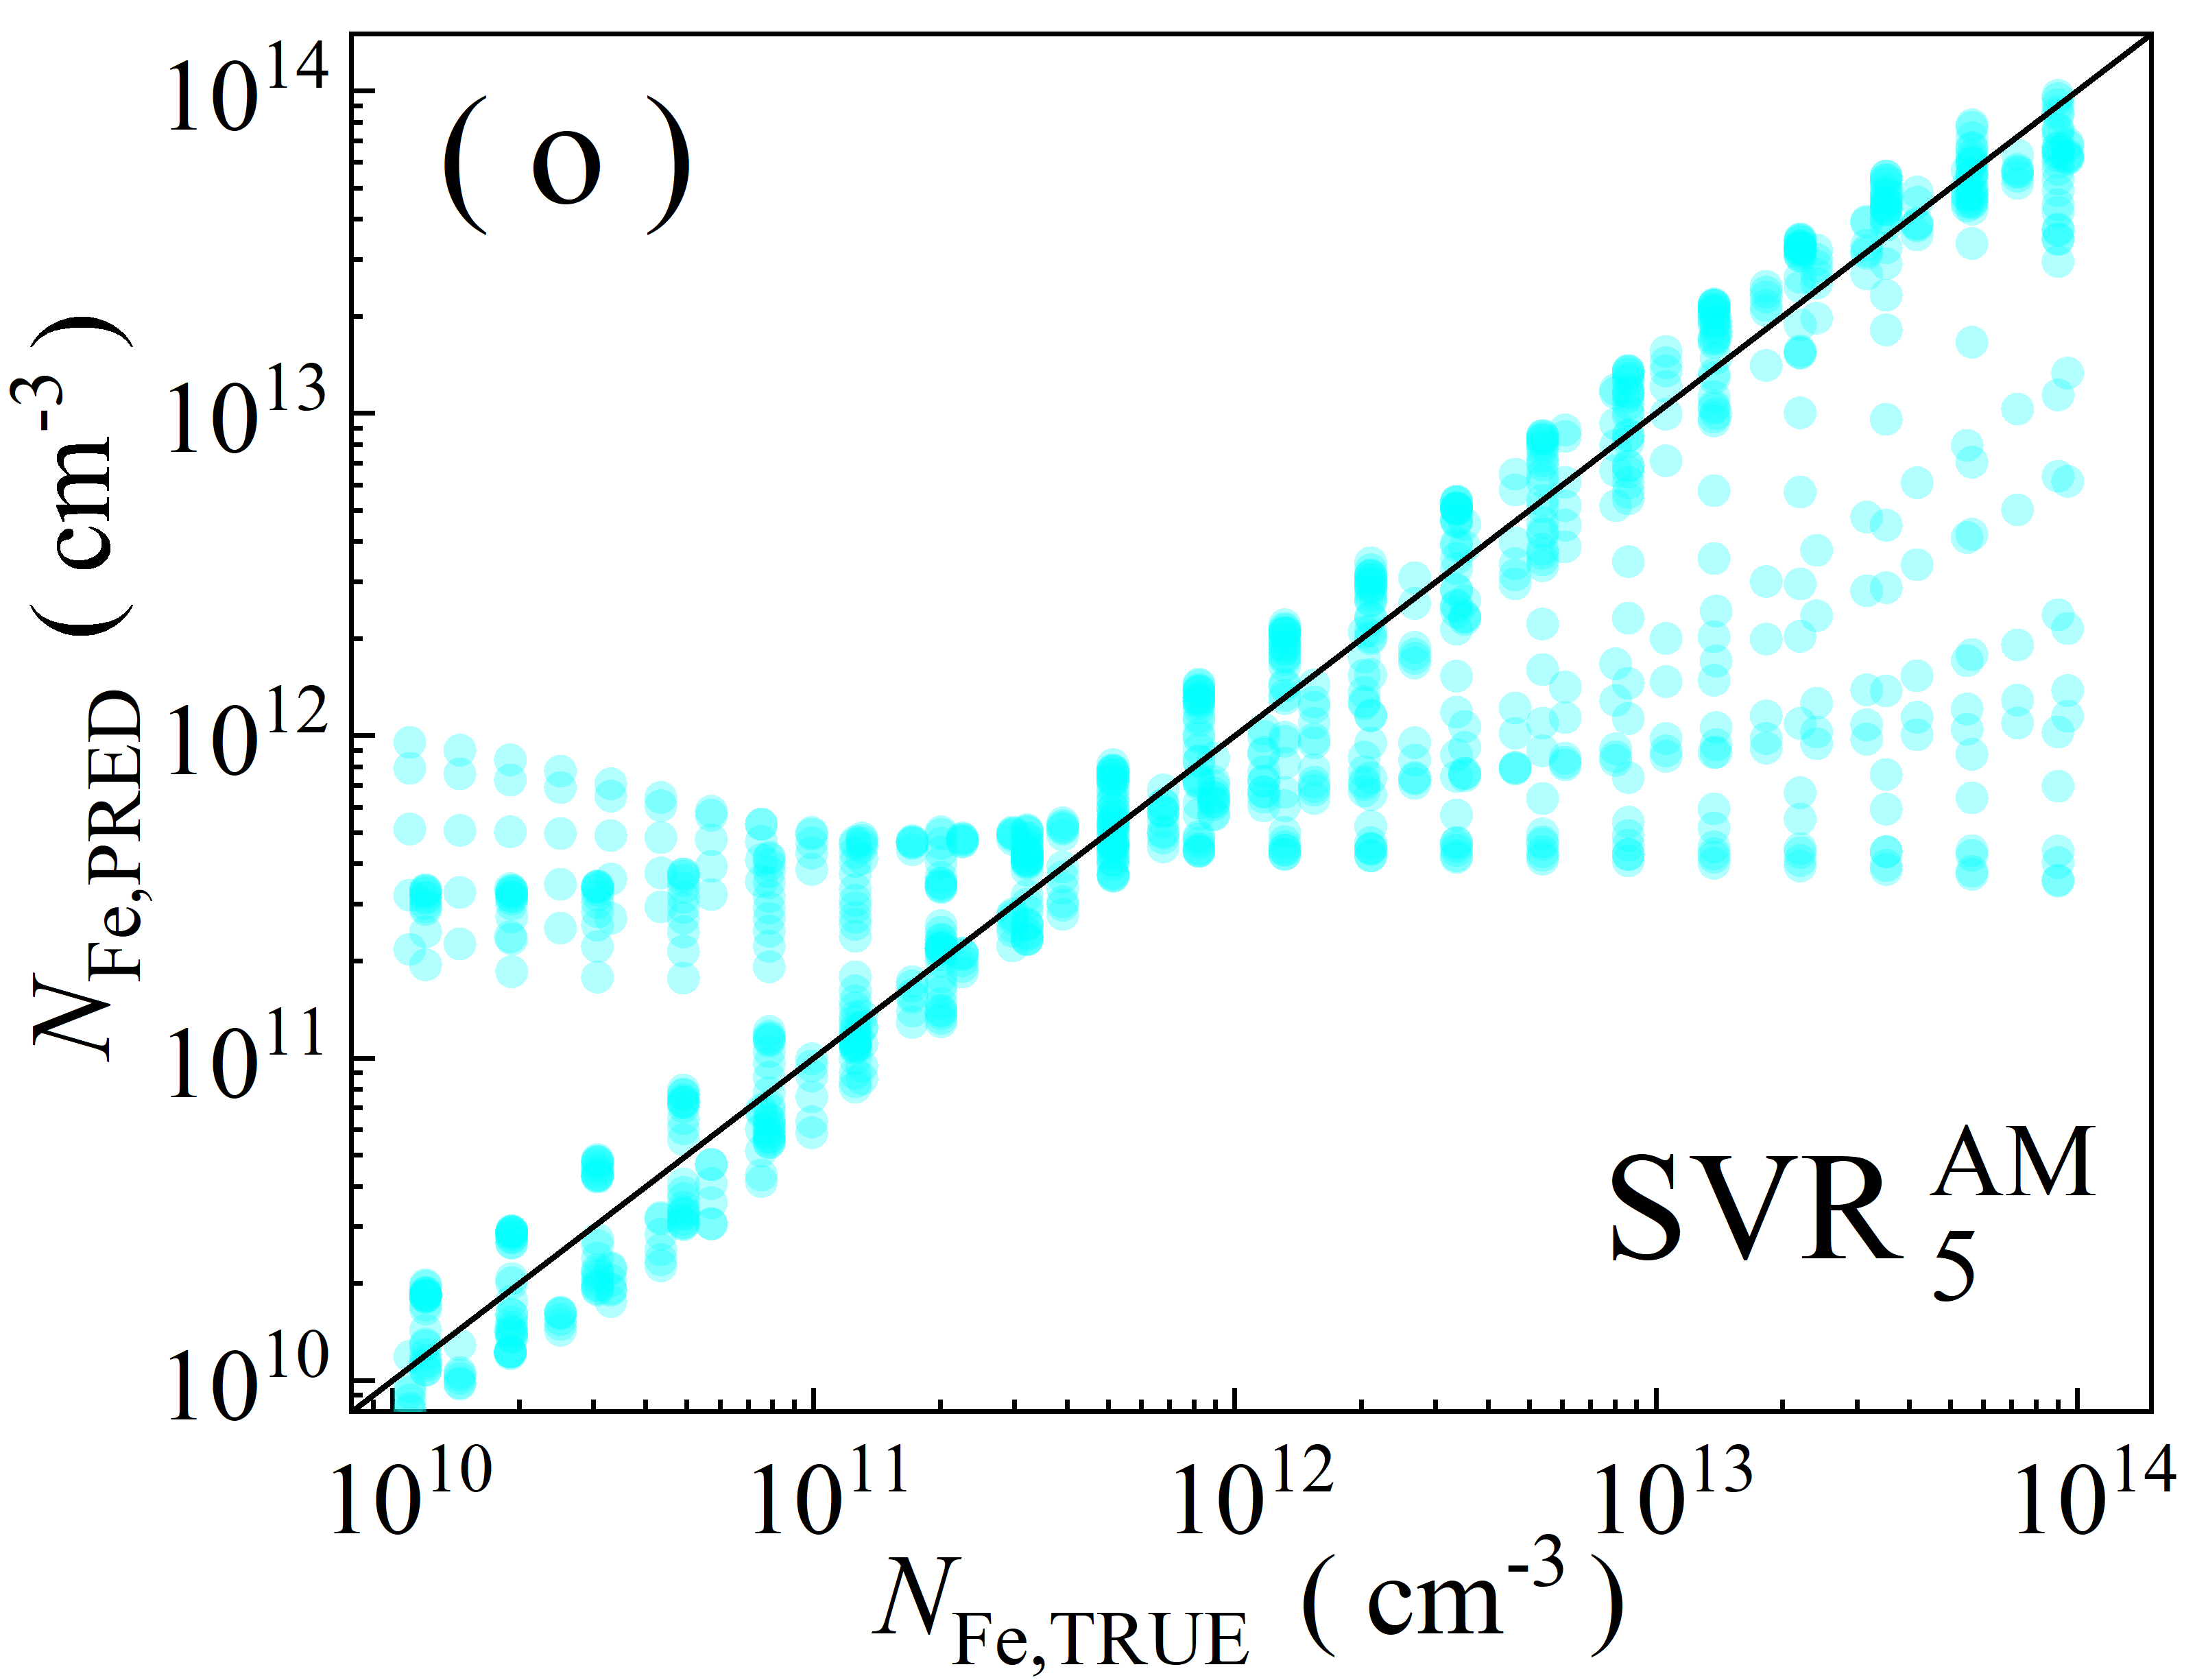
\includegraphics[width=0.24\linewidth]{Fig6o.png}
     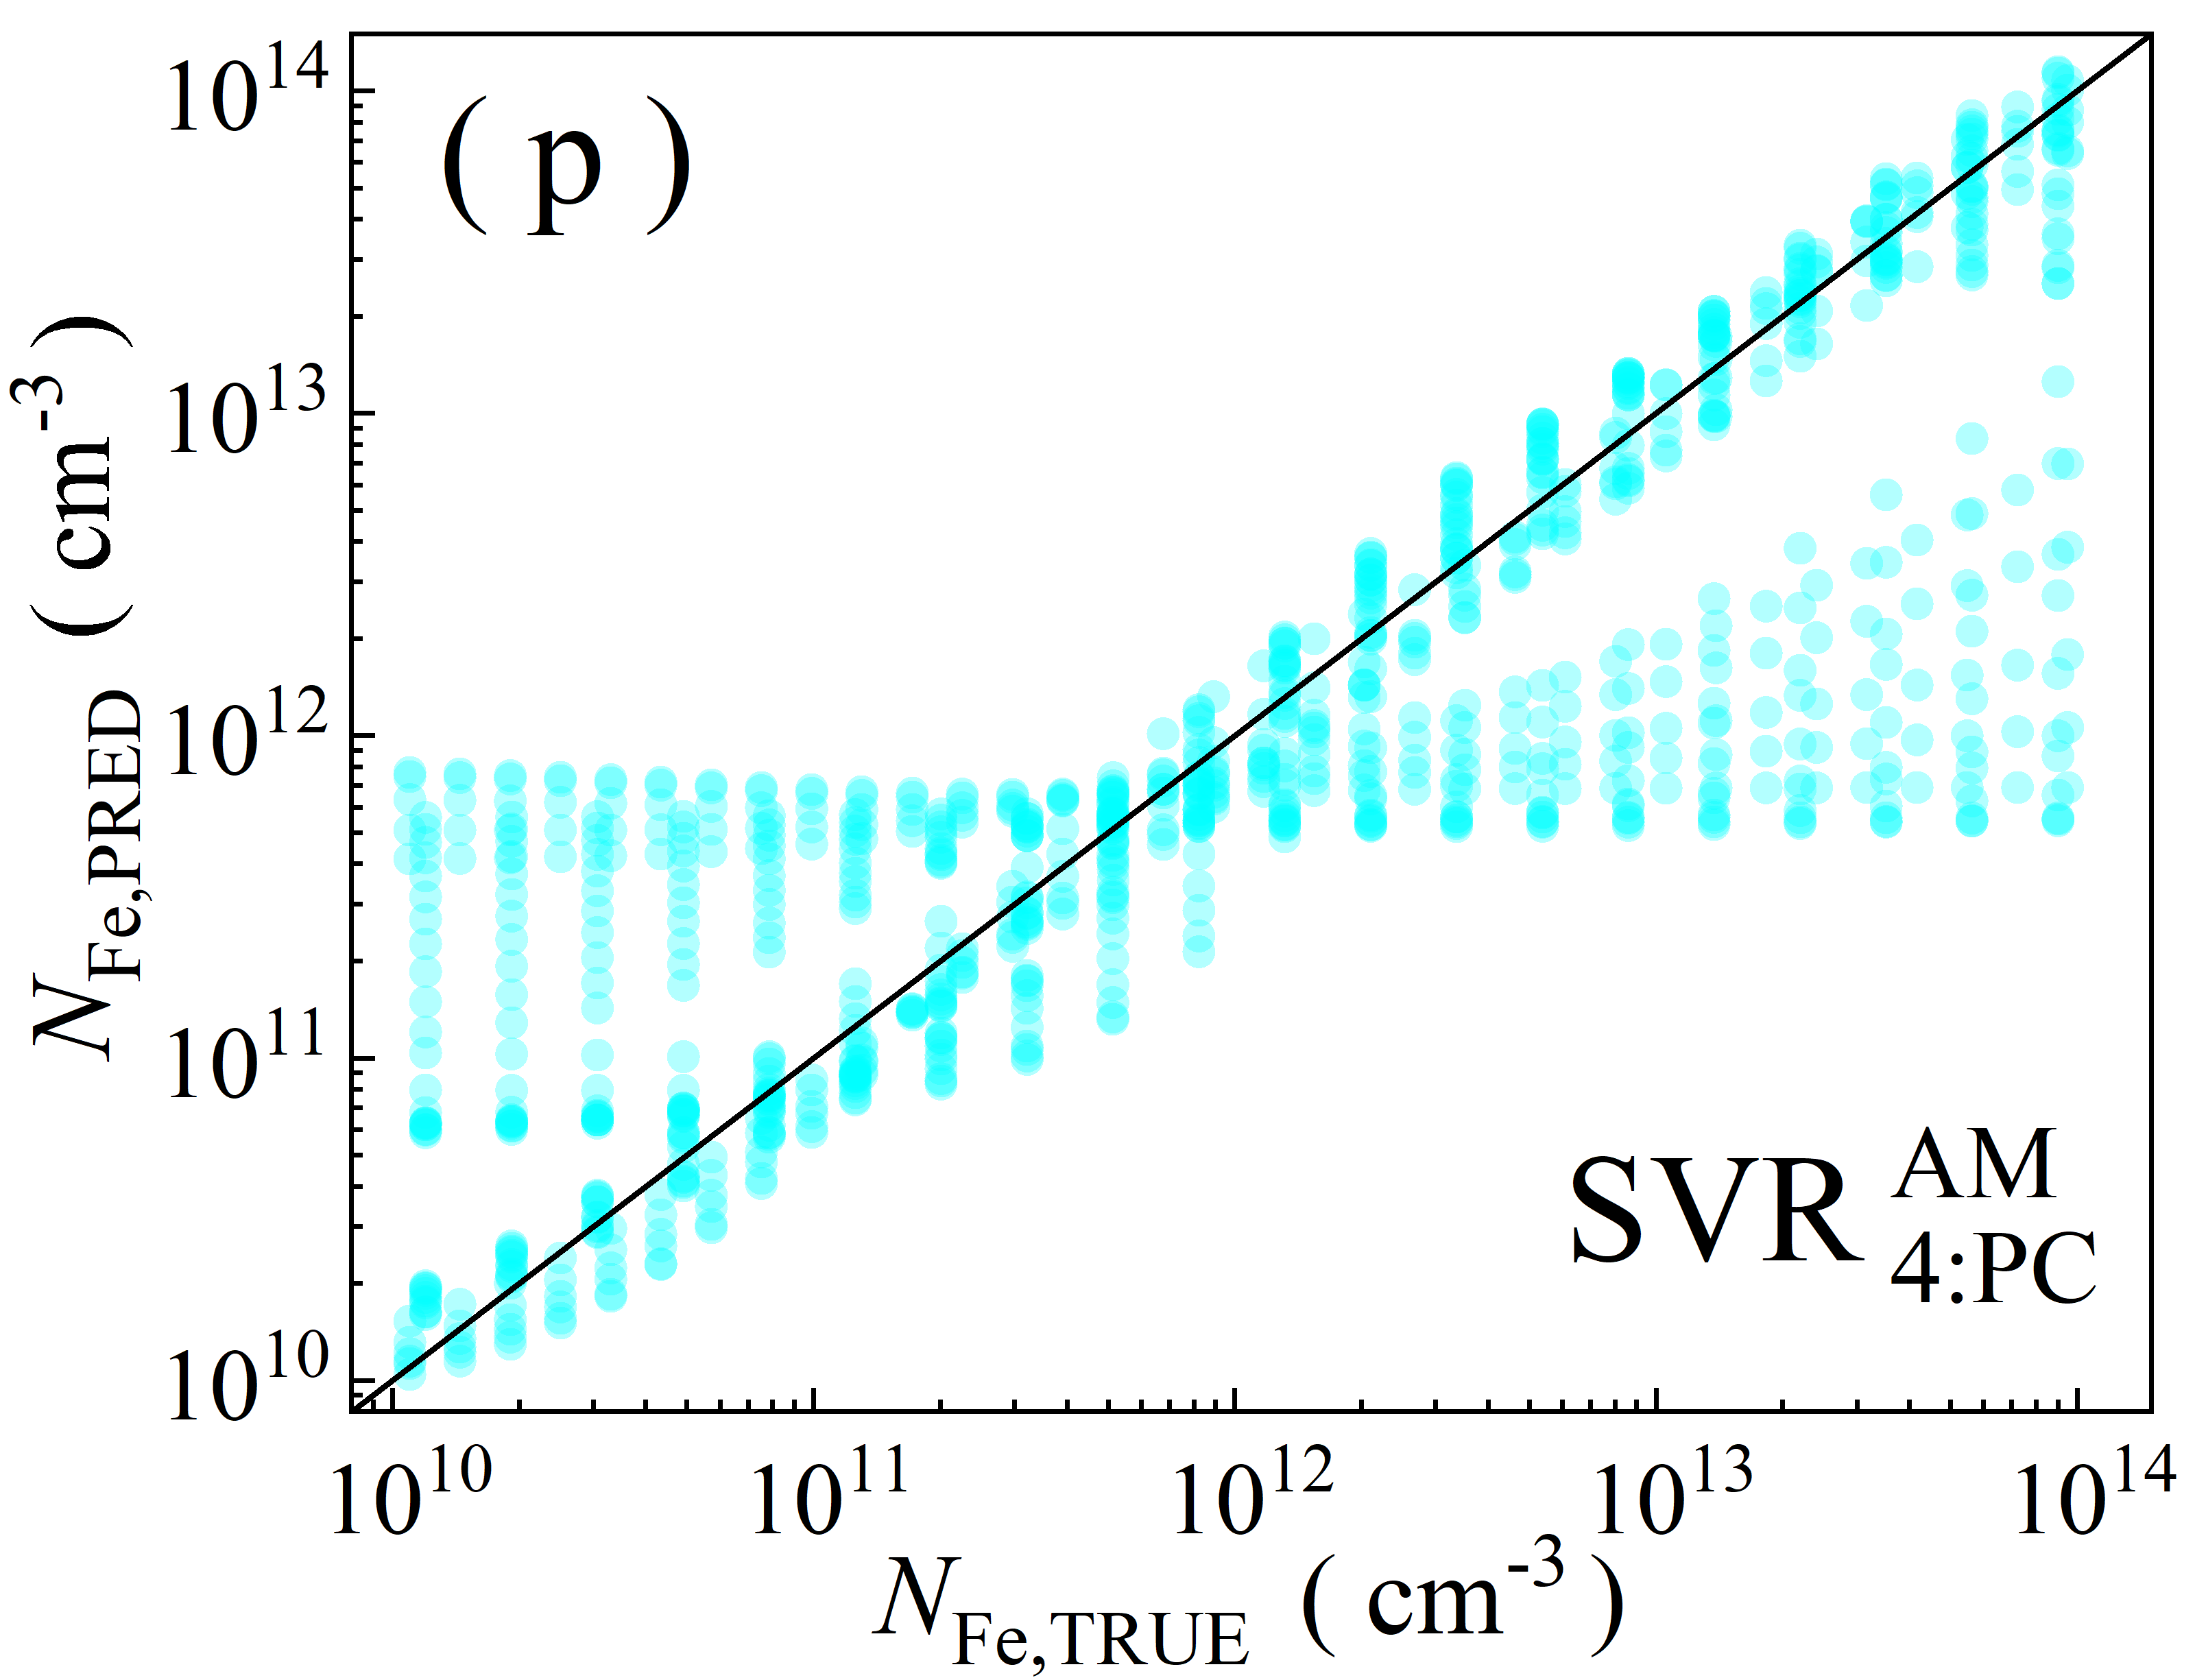
\includegraphics[width=0.24\linewidth]{Fig6p.png}
     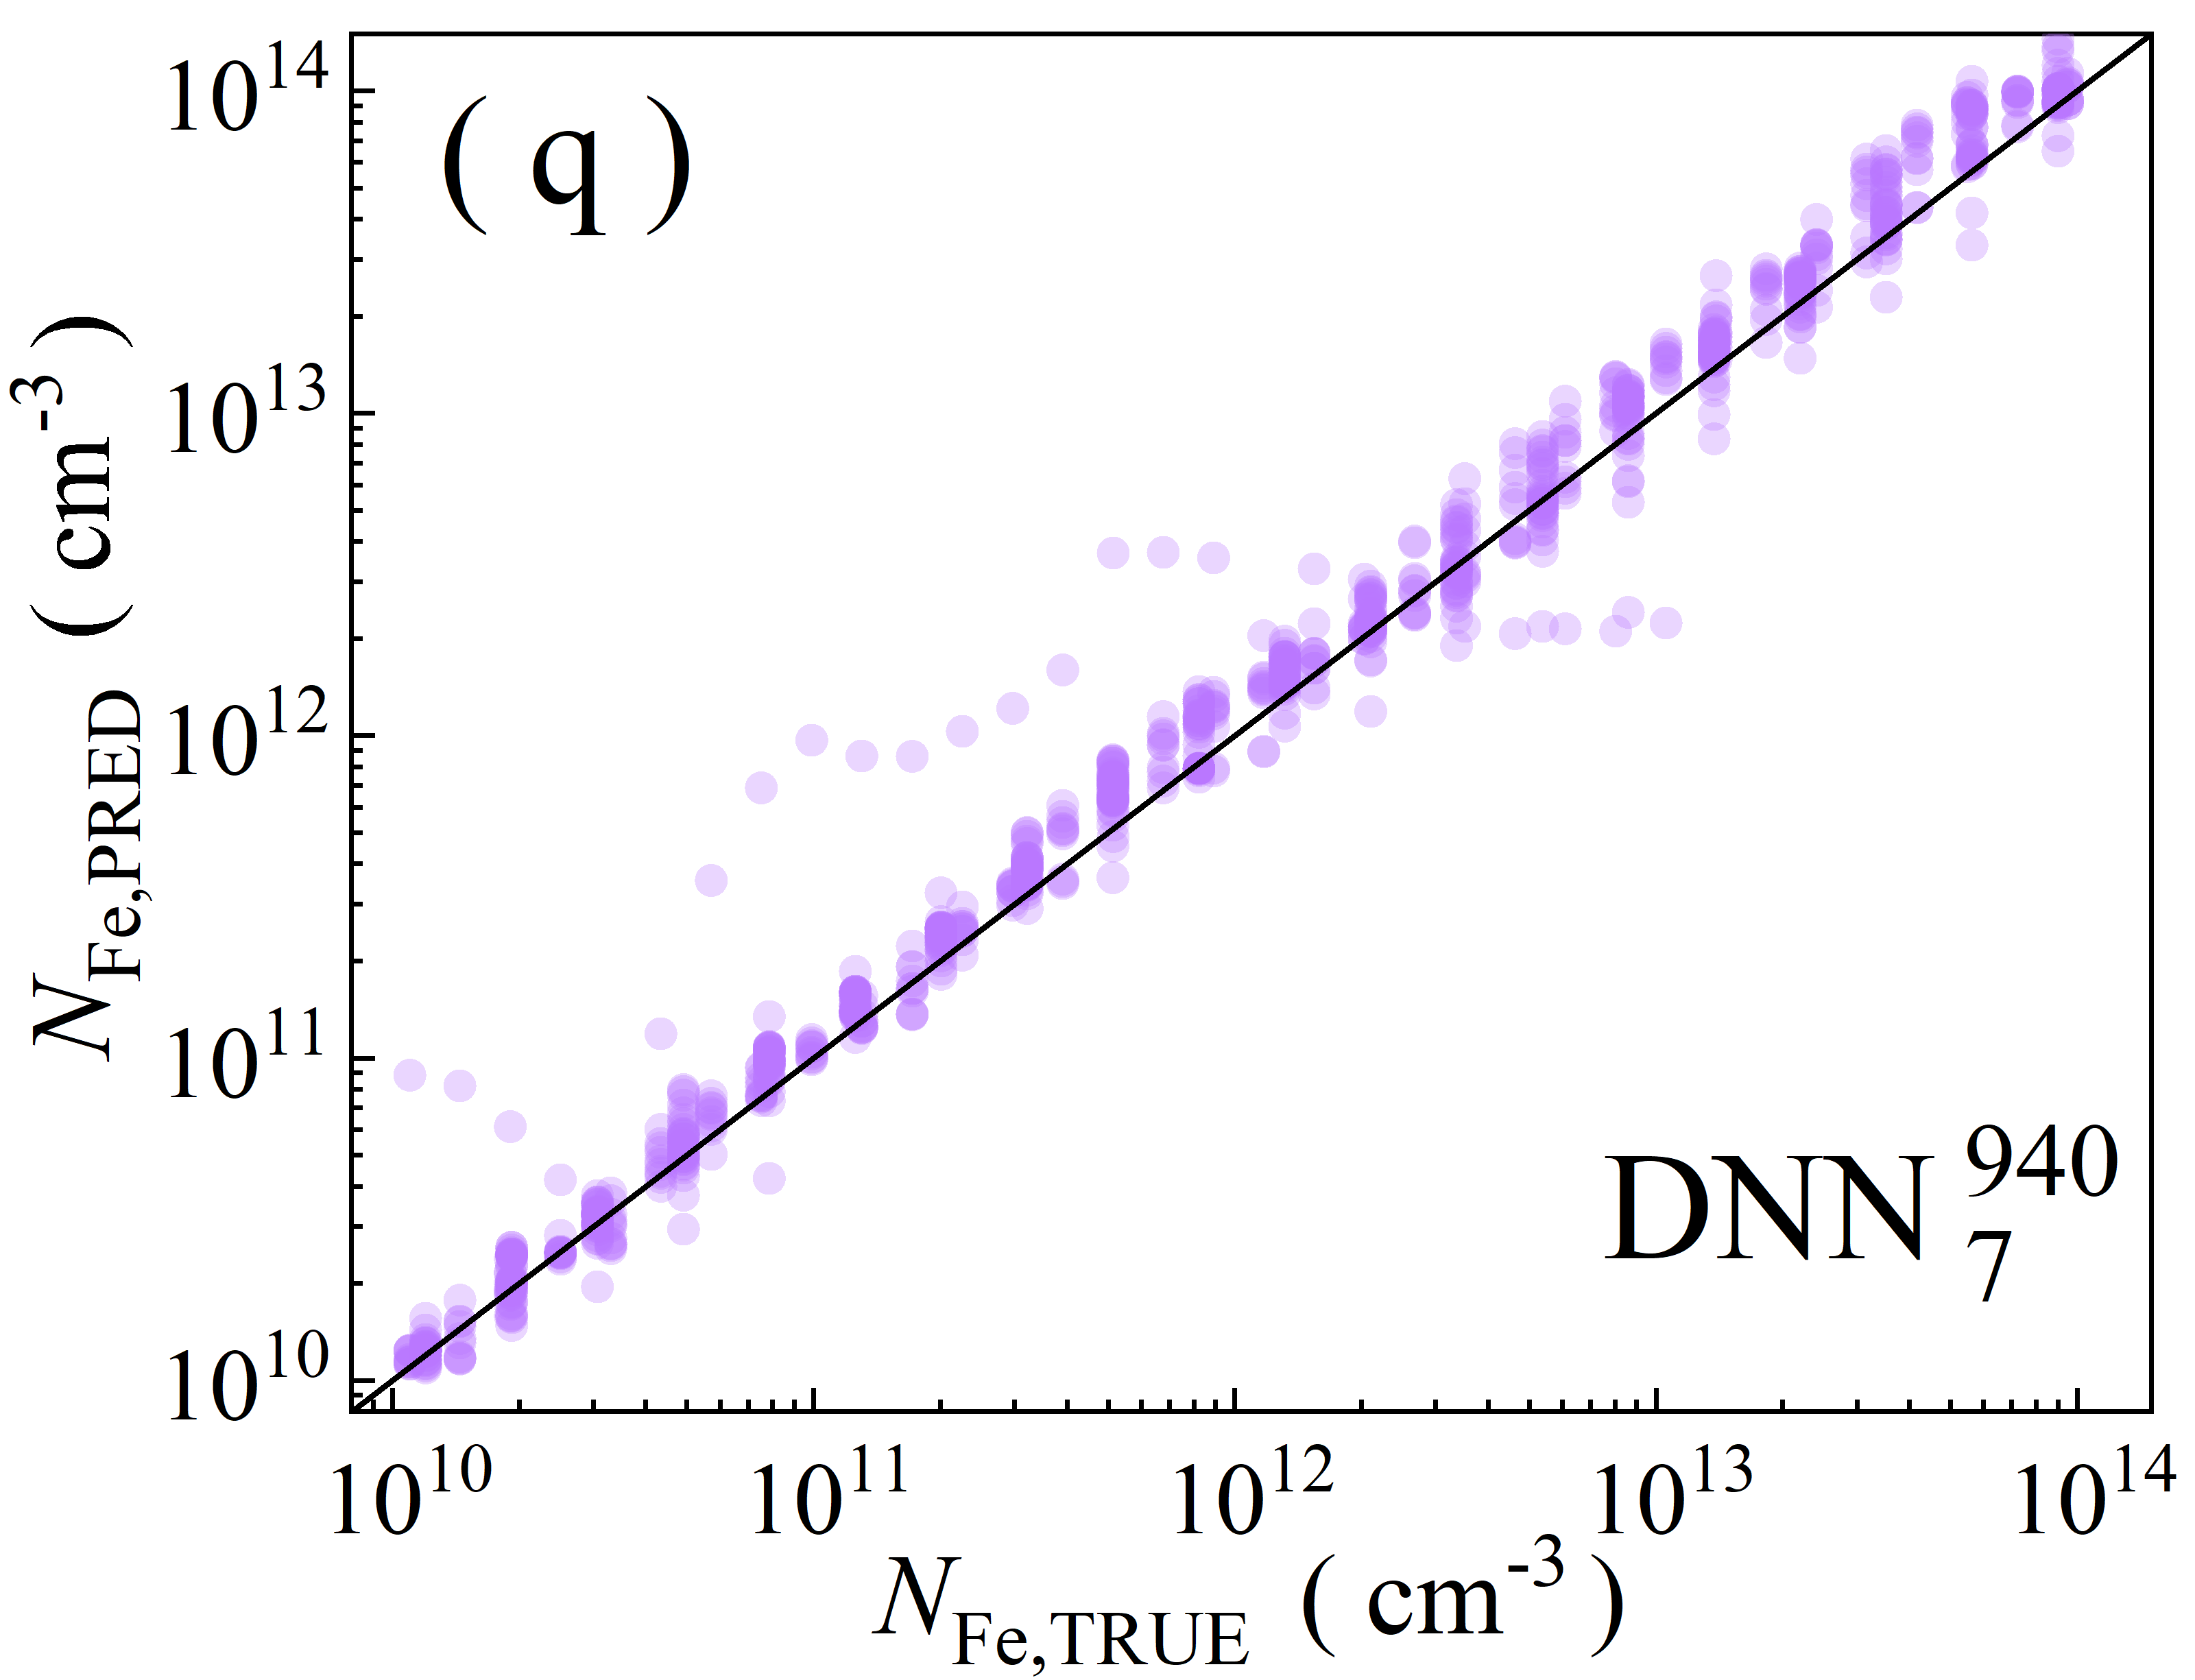
\includegraphics[width=0.24\linewidth]{Fig6q.png}
     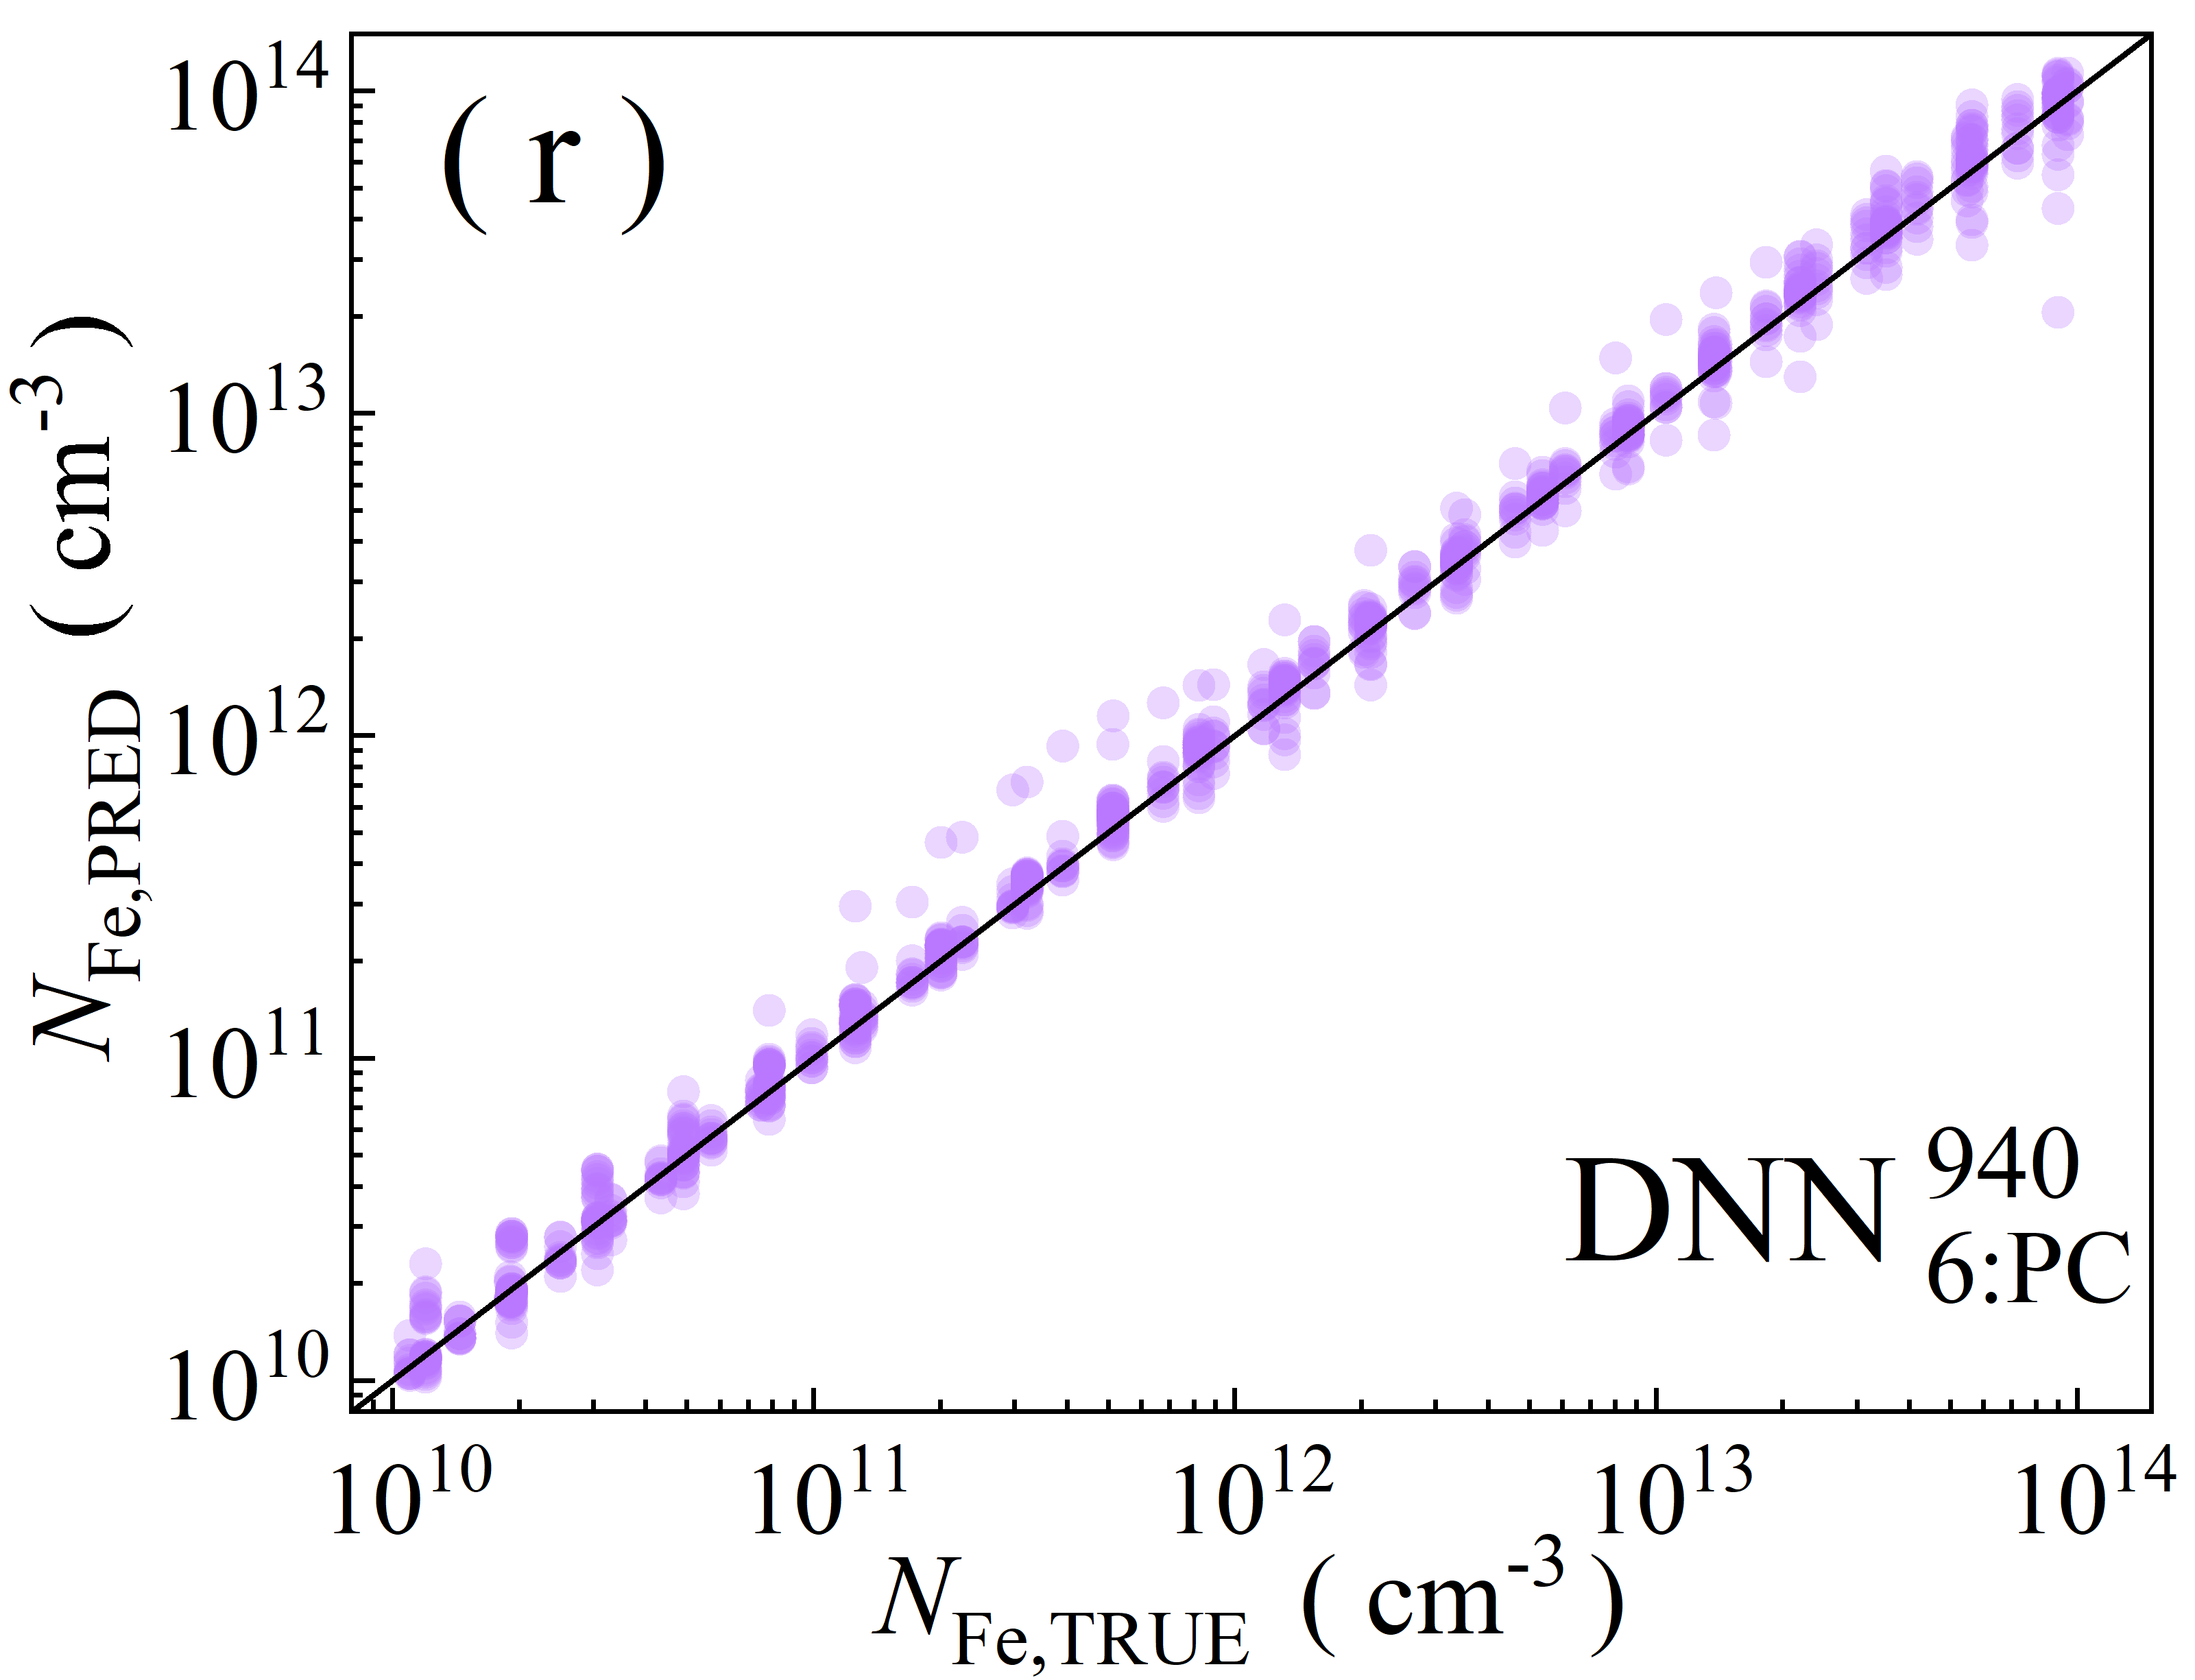
\includegraphics[width=0.24\linewidth]{Fig6r.png}
     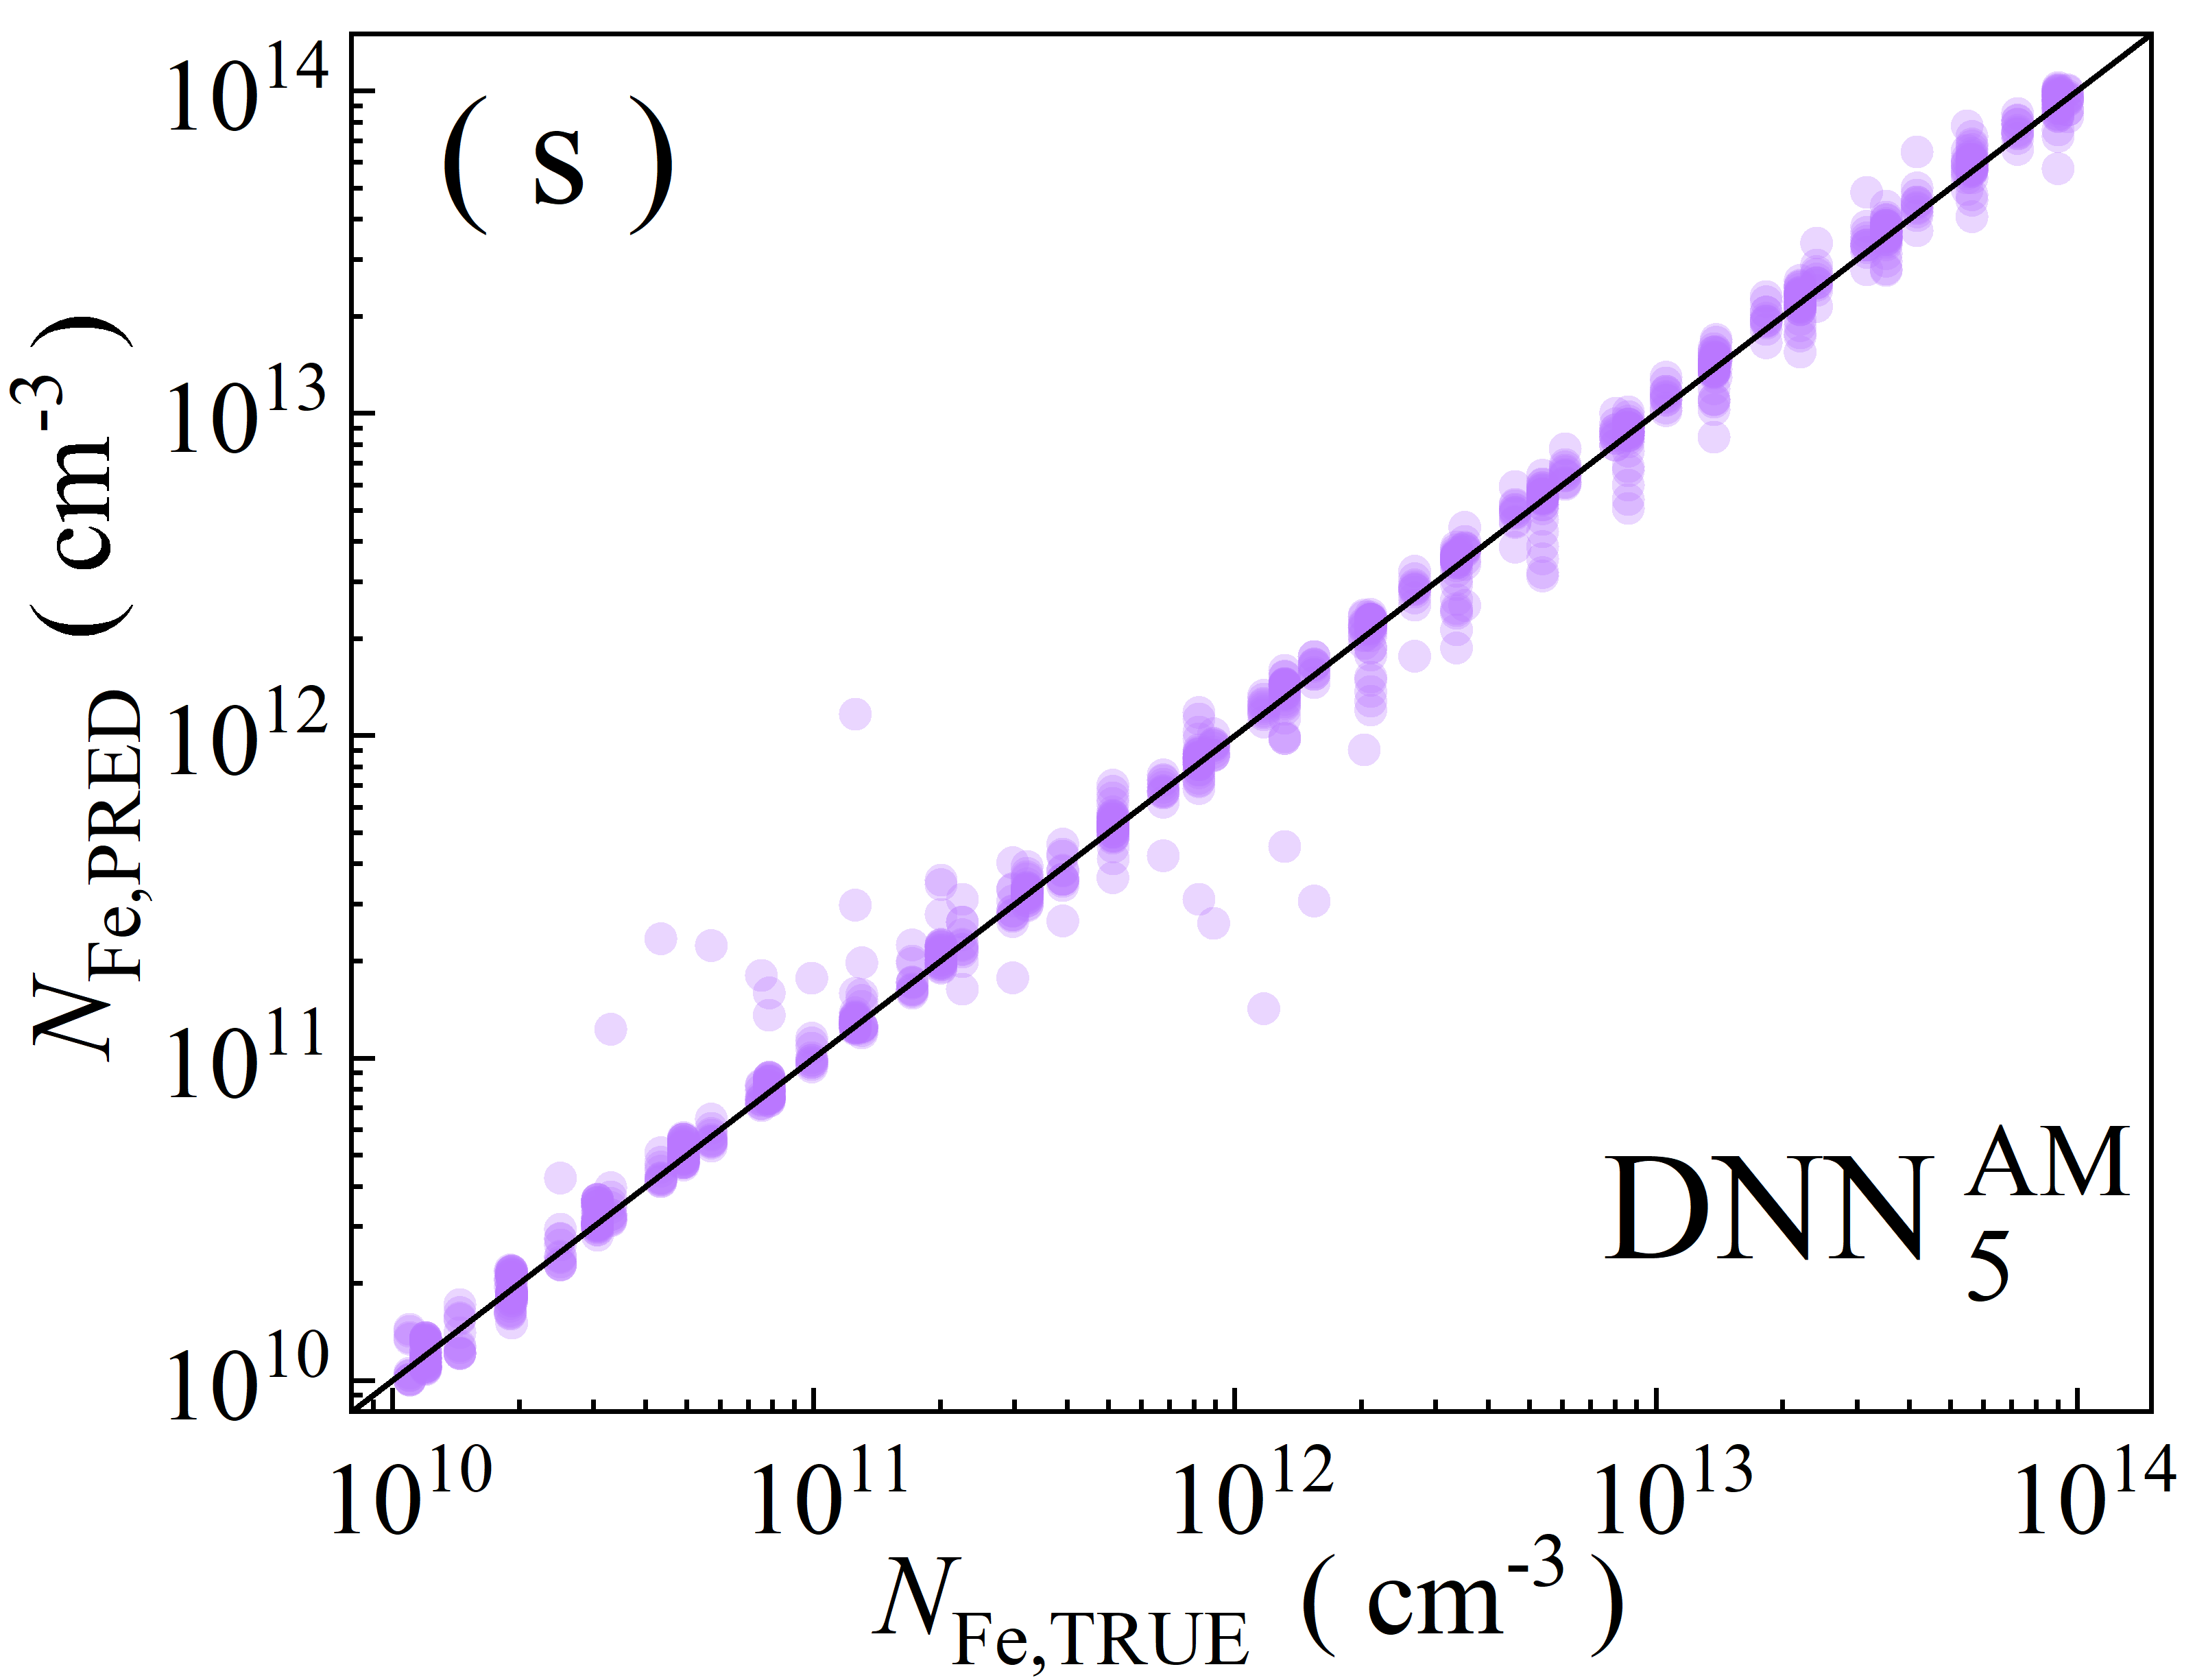
\includegraphics[width=0.24\linewidth]{Fig6s.png}
     \includegraphics[width=0.24\linewidth]{Fig6t.png}
	  \caption{Scatter plots compare reference iron concentrations with ML-predicted values during the $N_\mathrm{Fe}$--altered test phase.
The ML algorithms include RF (a-d), GB (e-h), XGB (i-l), SVR (m-p), and DNN (q-t).
The data come from simulation under monochromatic (a, b, e, f, i, j, m, n, q, r) and AM1.5 illumination (c, d, g, h, k, l, o, p, s, t).
Panels b, d, f, h, j, l, n, p, r, and t include PCA. The input feature dimensions are 7 (a, e, i, m, q), 6 (b, f, j, n, r), 5 (c, g, k, o, s), and 4 (d, h, l, p, t).
The black lines are the identified lines serving as the references.
}\label{fig6}
\end{figure}

\begin{figure}
	\centering
     \includegraphics[width=0.2\linewidth]{Fig7a.png}
     \includegraphics[width=0.2\linewidth]{Fig7b.png}
     \includegraphics[width=0.2\linewidth]{Fig7c.png}
     \includegraphics[width=0.2\linewidth]{Fig7d.png}
     \includegraphics[width=0.2\linewidth]{Fig7e.png}
     \includegraphics[width=0.2\linewidth]{Fig7f.png}
     \includegraphics[width=0.2\linewidth]{Fig7g.png}
     \includegraphics[width=0.2\linewidth]{Fig7h.png}
     \includegraphics[width=0.2\linewidth]{Fig7i.png}
     \includegraphics[width=0.2\linewidth]{Fig7j.png}
     \includegraphics[width=0.2\linewidth]{Fig7k.png}
     \includegraphics[width=0.2\linewidth]{Fig7l.png}
     \includegraphics[width=0.2\linewidth]{Fig7m.png}
     \includegraphics[width=0.2\linewidth]{Fig7n.png}
     \includegraphics[width=0.2\linewidth]{Fig7o.png}
     \includegraphics[width=0.2\linewidth]{Fig7p.png}
     \includegraphics[width=0.25\linewidth]{Fig7q.png}
     \includegraphics[width=0.25\linewidth]{Fig7r.png}
	  \caption{MSE (a--h), MAPE (i--p), and R$^{2}$ (q, r) scores for various models,
feature combinations, and illumination conditions on the $N_\mathrm{Fe}$--altered test dataset.
Illumination: 940~nm (a--d, i--l, q), AM1.5 (e--h, m--p, r).
Feature dimensions: 4 (a, e, i, m), 5 (b, f, j, n), 6 (c, g, k, o), and 7 (d, h, l, p).
Results with PCA are shown as circles (a--h) and shaded areas (i--r),
while results without PCA are represented by squares (a--h) and filled regions (i--r).
The numbers in panels (a--h) represent MSE values multiplied by 1000,
while the numbers in panels (i--p) indicate MAPE values in percentage.
}\label{fig7}
\end{figure}


\begin{table}[<options>]
\caption{Performance metrics of the ML models for $N_\mathrm{Fe}$--altered dataset}
\label{table2}
\begin{tabular*}{\tblwidth}{@{}CCCCCCCCCCCCCC@{}}
\toprule
\multirow{3}{*}{Algorithm}&\multirow{3}{*}{\makecell{Feature \\ dimension}}&\multicolumn{4}{C}{MdAPE (\%)}&\multicolumn{4}{C}{$p01$ (\%)}&\multicolumn{4}{C}{$p10$ (\%)}\\
&&\multicolumn{2}{C}{940 nm}&\multicolumn{2}{C}{AM1.5}&\multicolumn{2}{C}{940 nm}&\multicolumn{2}{C}{AM1.5}&\multicolumn{2}{C}{940 nm}&\multicolumn{2}{C}{AM1.5}\\
&&Init&PCA&Init&PCA&Init&PCA&Init&PCA&Init&PCA&Init&PCA\\
\midrule
RF& 4 & 6.47 & 6.38 & 8.29 & 8.00 & 10.1& 9.48& 7.54& 8.12& 68.0& 70.2& 57.0 & 57.9\\
& 5& 7.67& \textbf{6.00}& 6.96& 9.46& 7.06& 8.51& 10.1& 6.96& 60.5& 72.2& 64.2& 52.1\\
& 6& 8.01 & 7.34 & 5.46& 5.66& 6.58 & 7.74& 11.0& 10.9& 59.5& 60.4& 72.4& 72.9\\
& 7& 8.89& 8.74& 6.27& 4.62& 5.71& 5.42& 10.4& 13.3& 54.2& 56.4& 68.8& 82.2\\
GB&4&4.63&4.35&6.95&6.27&\textbf{13.6}&\textbf{14.1}&9.87&9.38&76.5&80.3&62.4&67.2\\
&5&4.96&4.63&6.55&8.05&\textbf{13.6}&12.5&11.2&7.25&72.7&\textbf{82.4}&66.6&57.4\\
&6&6.78&6.73&5.31&4.41&8.03&9.09&11.9&15.4&65.5&64.0&74.4&79.1\\
&7&7.87&7.41&4.97&3.73&7.16&7.64&12.2&17.4&60.7&61.8&75.3&84.3\\
XGB&4&4.82&6.91&6.43&7.75&11.0&9.77&10.1&8.32&75.6&63.5&62.7&60.2\\
&5&\textbf{4.46}&6.20&4.26&9.04&11.7&10.2&13.8&6.58&\textbf{78.6}&68.6&74.7&52.3\\
&6&6.49&7.57&4.13&4.79&9.87&8.51&14.8&11.8&68.7&59.9&83.2&77.2\\
&7&6.16&7.96&3.71&3.94&8.80&7.54&15.2&15.6&66.0&60.9&83.3&83.0\\
SVR&4&31.1&26.7&41.2&40.5&1.45&1.35&1.06&0.77&14.9&18.2&11.4&11.8\\
&5&36.3&42.7&39.7&51.9&1.64&0.87&1.74&1.35&14.4&10.8&10.9&9.77\\
&6&37.0&44.8&37.3&44.2&1.16&0.48&1.64&0.77&13.4&8.99&14.4&10.1\\
&7&39.1&38.1&36.5&32.5&1.16&1.06&0.68&1.26&9.48&13.7&13.4&15.2\\
DNN&4&8.06&7.48&11.4&13.0&7.74&7.64&3.97&4.35&58.8&60.5&44.8&41.6\\
&5&7.42&9.02&5.97&6.84&6.48&6.67&10.1&6.77&66.0&54.7&72.3&61.4\\
&6&6.98&8.15&6.30&3.18&7.06&5.80&8.80&17.8&64.8&59.3&69.9&90.2\\
&7&17.3&6.93&\textbf{1.63}&\textbf{2.40}&4.06&8.90&\textbf{32.6}&\textbf{23.5}&33.1&64.7&\textbf{98.7}&\textbf{96.7}\\
\bottomrule
\end{tabular*}
\end{table}

When estimating iron concentration based on PVP variations obtained under AM1.5 illumination,
using only four descriptors does not yield sufficiently accurate predictions with any model.
However, adding efficiency variations (increasing the feature dimension from 4 to 5)
enables DNN and XGB to predict $N_\mathrm{Fe}$ with MAPE slightly above 10\%,
though the results remain inferior to those under monochromatic illumination.
The use of PCA significantly worsens the results (see Fig.~\ref{fig7}f, Fig.~\ref{fig7}n, Table~\ref{table2}).
A further increase in feature dimensionality improves prediction accuracy and reduces the performance gap between models with and without PCA.
The best results are observed when using seven descriptors.
For RF and GB, applying PCA decreases both the mean errors (Fig.~\ref{fig7}p)
and the proportion of predictions with large deviations from the true values (Table~\ref{table2}).
For XGB and DNN --- the most efficient models across the entire $N_\mathrm{Fe}$--altered test dataset,
including data under 940~nm illumination --- PCA provides no benefit (Fig.~\ref{fig7}p, Fig.~\ref{fig8}b).
Notably, in these cases, the proportion of predictions with accuracy below 10\% does not exceed 1.3\%.

\begin{figure}
  \centering
     \includegraphics[width=0.4\linewidth]{Fig8a.png}
     \includegraphics[width=0.4\linewidth]{Fig8b.png}
    \caption{The proportion of samples in the $N_\mathrm{Fe}$--altered dataset with an absolute error below a given threshold, plotted as a function of the threshold value.
}\label{fig8}
\end{figure}

These results underscore the importance of selecting an optimal model and applying appropriate data preprocessing
to achieve accurate iron concentration predictions in silicon solar cells.


\subsection{$T$--altered test dataset}

The $T$-altered test dataset simulates a scenario in which impurity concentration estimates
are based on measurements taken under conditions different from those used for model training.
Additionally, this dataset includes temperature values (287~K, 341~K, and 342~K)
that extend beyond the training range $(290-340)$~K, enabling an assessment of the models' extrapolation capability.

Figs.~S12-S15 present the prediction results, while Fig.~\ref{fig9} and Table~\ref{table3} summarize the performance metrics.
The data show that the average metrics for all models worsen slightly compared
to the $N_\mathrm{Fe}$--altered dataset (Fig.~\ref{fig7}, Fig.~\ref{fig9}).
In most cases, PCA reduces model performance, except for AM1.5 at a feature dimensionality of 7.
For the 940~nm case, using six descriptors proves more effective than using four, as observed in the previous test dataset.

\begin{figure}
	\centering
     \includegraphics[width=0.2\linewidth]{Fig9a.png}
     \includegraphics[width=0.2\linewidth]{Fig9b.png}
     \includegraphics[width=0.2\linewidth]{Fig9c.png}
     \includegraphics[width=0.2\linewidth]{Fig9d.png}
     \includegraphics[width=0.2\linewidth]{Fig9e.png}
     \includegraphics[width=0.2\linewidth]{Fig9f.png}
     \includegraphics[width=0.2\linewidth]{Fig9g.png}
     \includegraphics[width=0.2\linewidth]{Fig9h.png}
     \includegraphics[width=0.2\linewidth]{Fig9i.png}
     \includegraphics[width=0.2\linewidth]{Fig9j.png}
     \includegraphics[width=0.2\linewidth]{Fig9k.png}
     \includegraphics[width=0.2\linewidth]{Fig9l.png}
     \includegraphics[width=0.2\linewidth]{Fig9m.png}
     \includegraphics[width=0.2\linewidth]{Fig9n.png}
     \includegraphics[width=0.2\linewidth]{Fig9o.png}
     \includegraphics[width=0.2\linewidth]{Fig9p.png}
     \includegraphics[width=0.25\linewidth]{Fig9q.png}
     \includegraphics[width=0.25\linewidth]{Fig9r.png}
	  \caption{MSE (a--h), MAPE (i--p), and R$^{2}$ (q, r) scores for various models, feature combinations,
and illumination conditions on the $T$--altered test dataset.
Illumination: 940~nm (a--d, i--l, q), AM1.5 (e--h, m--p, r).
Feature dimensions: 4 (a, e, i, m), 5 (b, f, j, n), 6 (c, g, k, o), and 7 (d, h, l, p).
Results with PCA are shown as circles (a--h) and shaded areas (i--r),
while results without PCA are represented by squares (a--h) and filled regions (i--r).
 The numbers in panels (a--h) represent MSE values multiplied by 1000, while the numbers in panels (i--p) indicate MAPE values in percentage.
}\label{fig9}
\end{figure}



\begin{table}[<options>]
\caption{Performance metrics of the ML models for $T$--altered dataset}
\label{table3}
\begin{tabular*}{\tblwidth}{@{}CCCCCCCCCCCCCC@{}}
\toprule
\multirow{3}{*}{Algorithm}&\multirow{3}{*}{\makecell{Feature \\ dimension}}&\multicolumn{4}{C}{MdAPE (\%)}&\multicolumn{4}{C}{$p01$ (\%)}&\multicolumn{4}{C}{$p10$ (\%)}\\
&&\multicolumn{2}{C}{940 nm}&\multicolumn{2}{C}{AM1.5}&\multicolumn{2}{C}{940 nm}&\multicolumn{2}{C}{AM1.5}&\multicolumn{2}{C}{940 nm}&\multicolumn{2}{C}{AM1.5}\\
&&Init&PCA&Init&PCA&Init&PCA&Init&PCA&Init&PCA&Init&PCA\\
\midrule
RF&4&6.50&13.1&\textbf{1.88}&11.6&18.2&8.92&\textbf{28.1}&11.8&60.4&40.8&\textbf{95.6}&45.2\\
&5&5.59&13.2&9.58&5.90&22.4&6.75&12.1&16.6&62.9&40.7&51.3&62.7\\
&6&4.61&13.3&14.2&2.13&20.8&8.58&9.50&35.3&68.8&43.5&42.1&77.3\\
&7&5.07&9.82&5.05&\textbf{1.94}&21.5&12&17.7&38.7&67.4&50.4&68.3&79.8\\
GB&4&5.29&12.5&3.47&10.1&20.7&6.67&21.5&5.08&62.0&42.9&80.6&49.8\\
&5&4.91&12.6&9.34&4.89&19.1&7.00&6.58&22.5&66.2&44.7&51.8&65.0\\
&6&3.41&9.12&12.8&1.81&22.3&11.2&4.67&\textbf{40.9}&73.1&52.4&43.2&78.3\\
&7&5.03&9.72&5.14&2.44&15.6&10.2&13.9&31.3&68.3&51.0&70.7&79.3\\
XGB&4&5.03&10.9&3.40&8.72&22.8&8.92&20.8&8.42&64.6&46.9&80.8&53.8\\
&5&3.64&9.01&9.88&5.14&28.4&8.75&7.00&23.7&67.3&53.0&50.3&66.3\\
&6&\textbf{2.47}&10.4&10.5&2.08&\textbf{33.6}&6.75&6.58&34.4&\textbf{73.7}&49.2&48.6&78.0\\
&7&9.93&\textbf{5.37}&5.78&3.38&9.92&\textbf{14.9}&12.3&19.3&50.3&\textbf{67.9}&69.2&78.3\\
SVR&4&30.9&27.8&5.11&36.4&1.50&1.58&13.6&0.67&15.3&18.3&72.9&12.8\\
&5&33.7&38.0&35.7&37.5&1.75&1.00&1.17&0.92&15.3&12.9&13.5&12.8\\
&6&38.3&40.9&47.6&37.1&1.50&1.50&0.67&1.25&14.3&15.0&9.83&12.8\\
&7&18.6&6.85&46.2&36.3&3.83&7.50&0.75&1.83&29.8&66.3&9.58&15.4\\
DNN&4&6.92&7.54&10.5&14.2&7.83&8.33&4.58&4.67&65.3&59.0&47.3&37.2\\
&5&6.53&8.90&5.46&7.44&9.17&5.50&10.9&7.42&68.8&53.8&71.6&58.4\\
&6&7.09&7.18&4.92&2.99&7.50&9.25&10.7&18.3&66.8&61.1&79.2&90.9\\
&7&39.3&35.9&32.2&2.53&1.25&1.50&1.00&23.2&10.7&13.3&14.7&\textbf{92.5}\\
\bottomrule
\end{tabular*}
\end{table}

A comparison of Table~\ref{table2} and Table~\ref{table3} reveals that,
unlike the mean characteristics, MdAPE, $p01$, and $p10$ are often better than those in the $N_\mathrm{Fe}$--altered dataset.
For example, for $\mathrm{XGB}^{940}_{6}$, MdAPE and $p01$ reach 2.47\% and 33.6\%,
whereas in the previous case, the best values were 4.46\% and 13.6\%.
These differences in the behavior of MSE, MAPE, and R$^2$, compared to other performance metrics,
suggest a higher proportion of accurate predictions while increasing error values in less successful forecasts.
In other words, prediction disparity increases ---
the rich get richer, and the poor get poorer.

Fig.~\ref{fig10} illustrates the dependence of the proportion of predictions with an error below 10\% on temperature for the two training datasets.
Within the $(290-340)$~K range, where the networks were trained, both datasets exhibit similar $p10$ values and overall trends,
despite the temperature values in the $T$-altered test dataset differing from those used during training.
Specifically, $p10$ remains nearly independent of temperature, consistent with the trend observed in Fig.~\ref{fig5}d.
However, a slight deviation of just a few kelvins from the training range significantly reduces prediction accuracy.
This behavior highlights the models' limited extrapolation capability compared to their interpolation performance.
The degradation of the average metrics (MSE, MAPE, R$^2$) primarily results from lower prediction accuracy at temperatures beyond the training range.

\begin{figure}
  \centering
     \includegraphics[width=0.5\linewidth]{Fig10.png}
    \caption{Typical dependencies of the fraction of predictions with an accuracy within 10\%
    as a function of temperature for the $T$--altered and $N_\mathrm{Fe}$--altered datasets.
}\label{fig10}
\end{figure}

Thus, applying the models to measurement data obtained at temperatures
that slightly deviate from the training conditions but remain within the training range is justified.


\subsection{$N_\mathrm{B}$--altered and All-altered test datasets}\label{NBaltered}

The $N_\mathrm{B}$--altered dataset represents a case where a model trained on a specific type of solar cell is used to evaluate iron impurity concentration in photovoltaic converters with slightly different parameters. The boron concentration in the base is one of the parameters that can vary during the production process of PV devices. Therefore, the model's ability to adapt to these variations enhances its applicability to real-world manufacturing conditions.

The optimal performance of 16 models utilizing RF, GB, XGB, and DNN algorithms is shown in Figs.~\ref{fig11}a--\ref{fig11}d, respectively.
The remaining panels of Fig.~\ref{fig11} illustrate the MAPE values.
The Supplementary Materials (Figs.~S16--S20, Table~S14) provide more detailed prediction results.

\begin{figure}
	\centering
     \includegraphics[width=0.2\linewidth]{Fig11a.png}
     \includegraphics[width=0.2\linewidth]{Fig11b.png}
     \includegraphics[width=0.2\linewidth]{Fig11c.png}
     \includegraphics[width=0.2\linewidth]{Fig11d.png}
     \includegraphics[width=0.2\linewidth]{Fig11e.png}
     \includegraphics[width=0.2\linewidth]{Fig11f.png}
     \includegraphics[width=0.2\linewidth]{Fig11g.png}
     \includegraphics[width=0.2\linewidth]{Fig11h.png}
     \includegraphics[width=0.2\linewidth]{Fig11i.png}
     \includegraphics[width=0.2\linewidth]{Fig11j.png}
     \includegraphics[width=0.2\linewidth]{Fig11k.png}
     \includegraphics[width=0.2\linewidth]{Fig11l.png}
	  \caption{(a)--(d) Scatter plots comparing reference iron concentrations with ML--predicted values for the $N_\mathrm{B}$--altered dataset for the best models based on RF (a), GB (b), XGB (c), and DNN (d).
(e)--(l) MAPE scores for various models, feature combinations, and illumination conditions.
Illumination: 940~nm (e--h), AM1.5 (i--l).
Feature dimension: 4 (e, i), 5 (f, j), 6 (g, k), and 7 (h, l).
The numbers represent error values as percentages.
}\label{fig11}
\end{figure}

The most striking aspect is the subpar performance of the RF, GB, and XGB models, which had previously demonstrated stable and satisfactory accuracy,
at least for certain combinations of descriptors and illumination conditions.
Notably, even SVR models do not always produce the worst results.
The application of PCA slightly improves prediction accuracy,
except under monochromatic illumination with seven descriptors.
However, the overall error metrics remain excessively bad.
Another important finding is that the best predictive performance is achieved with six features,
even though incorporating the ideality factor does not enhance model accuracy.


DNN models exhibit the highest performance for the $N_\mathrm{B}$--altered dataset,
achieving results comparable to the best outcomes obtained for the $N_\mathrm{Fe}$--altered and
\textcolor[rgb]{1.00,0.07,0.00}{
\hl{$T$--altered}} datasets.
Specifically, the most accurate predictions occur under 940~nm illumination with four or five descriptors
and under AM1.5 illumination with six or seven descriptors.
The application of PCA improves results only when the feature dimension is six or seven.



At the same time, it is important to note that in DNN model predictions, approximately 10\% of forecasts
exhibit significant errors (greater than 50\%), as shown in Fig.\ref{fig11}d.
Fig.\ref{fig12}a illustrates the distribution of prediction errors for the $N_\mathrm{Fe}$--altered, $N_\mathrm{B}$--altered, and $T$--altered datasets.
While the dependencies remain similar for APE less than 10\%, for higher errors,
the dependence $p$ for the $N_\mathrm{Fe}$--altered dataset increases more slowly,
indicating a higher proportion of less accurate predictions in this case.
Fig.\ref{fig12}b presents the dependence of $p10$ on boron concentration across different test datasets.
The observed dependencies are similar to those in the training set (Fig.~\ref{fig5}b)
and highlight the most significant challenges for the developed models in predicting solar cells
with a base doping level around $10^{16}$~cm$^{-3}$.
However, for the $N_\mathrm{Fe}$--altered set, prediction accuracy in this problematic range is significantly lower,
resulting in a higher occurrence of poor-quality forecasts.
In contrast, for $N_\mathrm{B}<3\times10^{15}$~cm$^{-3}$, DNN models demonstrate adaptability to previously unknown doping levels.

\begin{figure}
  \centering
     \includegraphics[width=0.35\linewidth]{Fig12a.png}
     \includegraphics[width=0.35\linewidth]{Fig12b.png}
    \caption{The proportion of samples in the test dataset with an absolute error below a given threshold as a function of the threshold value (a)
    and the dependencies of the fraction of predictions with an accuracy not exceeding 10\% on the doping level for various test datasets (b).
    The vertical lines in panel (b) indicate the boron concentration values used in the training dataset.
}\label{fig12}
\end{figure}

The results of this section highlight the importance of training models with $N_\mathrm{B}$ values expected
in solar cells requiring iron quantification, particularly within the range $N_\mathrm{B}=(5\times10^{15}-3\times10^{16})$~cm$^{-3}$.
If it is necessary to use models trained on boron concentrations in the base that differ from those in the analyzed sample,
the DNN algorithm should be preferred.


Given the results obtained for the $N_\mathrm{B}$--altered dataset,
testing the All-altered dataset presented a notable challenge for the developed models,
as it aimed to assess their interpolation capabilities.
Notably, this dataset does not test extrapolation capabilities: all four features (including temperature),
which are unrelated to PVP modifications, have different magnitudes from those in the train dataset b
ut still fall within the corresponding range.
The All-altered dataset encapsulates most of the challenges that may arise under practical conditions when characterizing solar cells.

As in the previous case, Figs.~\ref{fig13}a--~\ref{fig13}d presents the best results from the four algorithmic families,
while Figs.~\ref{fig13}e--~\ref{fig13}l displays the MSE values.
Figs.~S21--S25 and Table~S15 provide additional statistical details.

\begin{figure}
	\centering
     \includegraphics[width=0.2\linewidth]{Fig13a.png}
     \includegraphics[width=0.2\linewidth]{Fig13b.png}
     \includegraphics[width=0.2\linewidth]{Fig13c.png}
     \includegraphics[width=0.2\linewidth]{Fig13d.png}
     \includegraphics[width=0.2\linewidth]{Fig13e.png}
     \includegraphics[width=0.2\linewidth]{Fig13f.png}
     \includegraphics[width=0.2\linewidth]{Fig13g.png}
     \includegraphics[width=0.2\linewidth]{Fig13h.png}
     \includegraphics[width=0.2\linewidth]{Fig13i.png}
     \includegraphics[width=0.2\linewidth]{Fig13j.png}
     \includegraphics[width=0.2\linewidth]{Fig13k.png}
     \includegraphics[width=0.2\linewidth]{Fig13l.png}
	  \caption{(a)--(d) Scatter plots comparing reference iron concentrations with ML--predicted values for the All--altered test dataset for the best models based on  RF (a), GB (b), XGB (c), and DNN (d).
(e)--(l) MSE scores for various models, feature combinations, and illumination conditions.
Illumination: 940~nm (e--h), AM1.5 (i--l).
Feature dimension: 4 (e, i), 5 (f, j), 6 (g, k), and 7 (h, l).
The numbers represent MSE values multiplied by 1000.
}\label{fig13}
\end{figure}


The presented data reveal several similarities between the results for the All--altered and $N_\mathrm{B}$--altered datasets:
i)~RF, GB, XGB, and SVR models exhibit low prediction accuracy; although PCA enhances accuracy, the improvement remains insufficient;
ii)~DNN models demonstrate relatively high average predictive performance, particularlywith four and five features under 940~nm illumination
and six features under AM1.5 illumination;
iii)~PCA reduces DNN model error when applied to datasets with six and seven features;
iv)~approximately 5\% of DNN predictions have APE~>~50\%.
These similarities suggest that the primary source of increased errors in the All--altered dataset
is the deviation of boron concentration values from those used in train phase.

\begin{tcolorbox}[highlight style]
\textcolor[rgb]{1.00,0.07,0.00}{
\subsection{Comparative Analysis}
}\end{tcolorbox}

\textcolor[rgb]{1.00,0.07,0.00}{
\hl{
Before presenting the results based on experimental data, a few summarizing remarks are in order.
One can see that models trained on data obtained under AM1.5 illumination perform worse in almost all cases.
We believe this can be attributed to the following reasons.
It is well known that a regression model may  achieve high accuracy
by having the target variable be an unambiguous function of the descriptor.
Moreover, the absolute value of the function’s derivative should be as significant as possible.
As shown earlier}  \cite{Olikh2025MSEB}, the condition of uniqueness in the relationship between $N_\mathrm{Fe}$ and
the changes in PVPs under AM1.5 illumination is often not fulfilled in contrast to the case of monochromatic illumination.
In addition, the ranges of changes in $\varepsilon I_\mathrm{SC}$, $\varepsilon V_\mathrm{OC}$, and $\varepsilon \eta$
under monochromatic illumination exceed those observed under AM1.5 illumination (see Subsection~\ref{SecDataCol}).
The physical origin of the differences in the relationship between iron concentration and
parameter changes under AM1.5 and monochromatic illumination lies in the fact that,
in the former case, the generation of non-equilibrium charge carriers occurs throughout the
entire volume of the solar cell, rather than being limited to the base region.
As a result, the processes involved in photovoltaic conversion are more complex.
In our view, these differences explain why the performance of ML models trained on AM1.5 illumination data is generally poorer.
One way to address the ambiguity in the relationship between features and the target variable
is to incorporate additional features into the model.
As it is shown, for AM1.5 illumination, increasing the number of descriptors often improves prediction accuracy, supporting our hypothesis.
}

\textcolor[rgb]{1.00,0.07,0.00}{
\hl{
Increasing the number of descriptors while keeping the sample size constant leads
to higher sparsity in the data space due to increased dimensionality,
which in turn makes it more difficult for the model to generalize.
In such cases, the model may also learn spurious correlations that do not generalize to test data ---
a risk that is particularly pronounced in deep neural networks and  deep tree-based ensemble methods.
Moreover, a larger number of features results in more model parameters, increasing the risk of overfitting.
These factors can collectively lead to a reduction in prediction accuracy.
In our opinion, for A$^\mathrm{AM1.5}$ models, both the positive effects achieved by increasing the number of descriptors
(enhancing overall information variance and reducing ambiguity between the target variable and the input features) were dominant.
However, for A$^\mathrm{940}$ models where this ambiguity was already low,
the negative effects described above outweighed the benefits,
which explains why prediction accuracy did not improve when using an expanded feature set.
}}




\textcolor[rgb]{1.00,0.07,0.00}{
\hl{
Another effect that may arise when increasing the number of features is multicollinearity.
It occurs when new features are highly correlated with existing ones and can lead to instability in model estimates.
However, in our case, it is unlikely that multicollinearity among the photovoltaic parameters
(incidentally, their correlation is significantly higher in the 940 nm case than in the AM1.5 case — see Fig.~S1)
affects prediction accuracy.
First, all algorithms used are sufficiently robust to multicollinearity.
Second, a standard method for mitigating multicollinearity is PCA.
Despite previous successes in applying principal component analysis to various
photovoltaics-related machine learning tasks} \cite{Gao2020,Fadhel2019,David2021,Liu2022,AbdullahVetter2025} ---
\hl{and the presence of favorable conditions for its use in our case,
such as the high correlation between changes in photoelectric parameters caused by FeB pair dissociation ---
applying PCA as a data pre-processing step for evaluating iron impurity concentration did not improve the maximum prediction accuracy in most cases.
One likely reason is that PCA preserves the overall variance in the data
but does not account for the specific relationships between individual features and the target variable.
For instance, some photovoltaic parameters may be more informative for predicting low iron concentrations,
while others may be more relevant for high concentrations.
For instance, $\varepsilon F\!F$) are shown} \cite{Olikh2025MSEB} to be most pronounced at low iron concentrations, unlike other PVPs.
When these components are merged through PCA transformation, such distinctions may be lost, leading to reduced accuracy.
Another possible reason is that principal components ---
being linear combinations of original features --- do not support localized decision splits
(i.e., those based on individual feature thresholds), which are particularly effective in tree-based models.
}

\textcolor[rgb]{1.00,0.07,0.00}{
\hl{
Rare cases where PCA pre-processing leads to improved prediction accuracy typically
occur when the original model (without PCA) performs poorly.
In this context, one might consider using PCA as a diagnostic indicator of model quality
when evaluating iron concentration in silicon solar cells:
if PCA improves prediction accuracy, it suggests that the baseline model is weak;
if not, the model is likely to be strong.
However, this approach relies on access to the true $N_\mathrm{Fe}$ values,
significantly restricting its practical applicability.
}}

\textcolor[rgb]{1.00,0.07,0.00}{
\hl{
When comparing the effectiveness of different algorithms, several points are worth noting.
The poorest performance observed with SVR is likely due to its limited ability
to model complex nonlinear relationships ---
such as those that apparently exist between iron concentration and variations in photoelectric parameters.
In contrast, the superior performance of the XGB and DNN models is attributable to
their ability to effectively capture nonlinear patterns, which in our case become more prominent with increasing descriptor dimensionality.
Specifically, XGB performs best in relatively simpler scenarios, such as those involving 940 nm illumination
(see Figs.}~\ref{fig7}i-\ref{fig7}l, \ref{fig9}i-\ref{fig9}l).
This is because XGB requires less training data than DNN
(12,000 examples are sufficient, though this is not a particularly large amount for a neural network),
handles high-quality structured data well (simulated data are noise-free),
and is more resilient to the influence of correlated features.
At the same time, DNNs are more powerful tools for nonlinear modeling,
capable of uncovering hidden structures in the data.
This enables them to achieve better results on more complex tasks ---
such as the transition to A$^\mathrm{AM1.5}$-models with high-dimensional features
(see Figs.~\ref{fig7}m-\ref{fig7}p, \ref{fig9}m-\ref{fig9}p).
As shown by the results in Subsection~\ref{NBaltered}, successful prediction within the
$N_\mathrm{B}$--altered also requires accounting for higher-order relationships,
which explains why DNN models achieved the best performance (Figs.~\ref{fig11}e-\ref{fig11}l).
Regarding the RF and GB algorithms, as indicated in Tables~\ref{table2} and \ref{table2},
they tend to perform best only on less complex data
(i.e., small sets of descriptors), where more powerful models are at higher risk of overfitting.
}


\subsection{Experimental validation}


To demonstrate the effectiveness of the proposed method, real solar cells were used.
The base thickness (380~$\mu$m) and the measurement temperatures (300, 305, 310, 320, 330, and 340~K) match those used in $I$-$V$ curve modeling for the train dataset.
However, the base doping level, $N_\mathrm{B}=1.36\times10^{15}$~cm$^{-3}$, was not among the $N_\mathrm{B}$ values used for training.
Therefore, the experimental test dataset is, to some extent, analogous to the $N_\mathrm{B}$--altered test dataset or even the $All$--altered dataset, considering the spread of iron concentration values.

That is, even before testing began, some difficulties with prediction based on measurement data could be foreseen (not only ML models can make predictions).
Meanwhile, the $N_\mathrm{B}$--altered test dataset included some data simulated for $N_\mathrm{B}=1.36\times10^{15}$~cm$^{-3}$.
Therefore, we tested the experimental data using following models:
i)~models trained on the training dataset for 940~nm illumination; these models had been previously validated on artificial test datasets;
ii)~models trained on all simulated data in monochromatic illumination case (full dataset), incorporating train, $N_\mathrm{Fe}$--altered,
$T$--altered, $N_\mathrm{B}$--altered, and All--altered test datasets.
In the latter case, we will use the following notation
\begin{equation*}
    \mathrm{A}^\mathrm{full}_\mathrm{feat},
\end{equation*}
where the upper index specifies the completeness of the data for training
and accounts for the fact that applying models trained for the AM1.5 case
to the experimental dataset is unjustified due to differing measurement conditions.

Fig.~\ref{fig14} and Figs.~S26--S29 present the prediction results of different models.
The experimental test datasets contained between 8 and 30 samples, with the exact number depending on the number of features.
The referenced figures display predictions for these datasets.
To ensure a more precise quantitative comparison, we analyzed a case where all models used an input dataset of the same size,
derived from $I$-$V$ measurements of the same solar cells.
The resulting performance metrics are shown in Fig.~\ref{fig15}.
The Supplementary Materials (Fig.~S30) also include averaged quantitative characteristics of model performance
across datasets of different sample sizes, which align with the trends observed in Fig.~\ref{fig15}.

\begin{figure}
	\centering
     \includegraphics[width=0.24\linewidth]{Fig14a.png}
     \includegraphics[width=0.24\linewidth]{Fig14b.png}
     \includegraphics[width=0.24\linewidth]{Fig14c.png}
     \includegraphics[width=0.24\linewidth]{Fig14d.png}
     \includegraphics[width=0.24\linewidth]{Fig14e.png}
     \includegraphics[width=0.24\linewidth]{Fig14f.png}
     \includegraphics[width=0.24\linewidth]{Fig14g.png}
     \includegraphics[width=0.24\linewidth]{Fig14h.png}
     \includegraphics[width=0.24\linewidth]{Fig14i.png}
     \includegraphics[width=0.24\linewidth]{Fig14j.png}
     \includegraphics[width=0.24\linewidth]{Fig14k.png}
     \includegraphics[width=0.24\linewidth]{Fig14l.png}
     \includegraphics[width=0.24\linewidth]{Fig14m.png}
     \includegraphics[width=0.24\linewidth]{Fig14n.png}
     \includegraphics[width=0.24\linewidth]{Fig14o.png}
     \includegraphics[width=0.24\linewidth]{Fig14p.png}
     \includegraphics[width=0.24\linewidth]{Fig14q.png}
     \includegraphics[width=0.24\linewidth]{Fig14r.png}
     \includegraphics[width=0.24\linewidth]{Fig14s.png}
     \includegraphics[width=0.24\linewidth]{Fig14t.png}
	  \caption{Scatter plots compare reference iron concentrations with ML--predicted values during the experimental test phase.
The ML algorithms include RF (a--d), GB (e--h), XGB (i--l), SVR (m--p), and DNN (q--t).
Panels (b, d, f, h, j, l, n, p, r, t) incorporate PCA pre-processing.
The input feature dimensions are 4 (a, b, i, j, q, r), 5 (e, f, m, n), 6 (c, d, k, l), and 7 (g, h, o, p, s, t).
The black lines are the identified lines serving as the references.
Marks with a black point inside correspond to models trained on the complete set of synthetic data.
}\label{fig14}
\end{figure}


\begin{figure}
	\centering
     \includegraphics[width=0.2\linewidth]{Fig15a.png}
     \includegraphics[width=0.2\linewidth]{Fig15b.png}
     \includegraphics[width=0.2\linewidth]{Fig15c.png}
     \includegraphics[width=0.2\linewidth]{Fig15d.png}
     \includegraphics[width=0.2\linewidth]{Fig15e.png}
     \includegraphics[width=0.2\linewidth]{Fig15f.png}
     \includegraphics[width=0.2\linewidth]{Fig15g.png}
     \includegraphics[width=0.2\linewidth]{Fig15h.png}
     \includegraphics[width=0.2\linewidth]{Fig15i.png}
     \includegraphics[width=0.2\linewidth]{Fig15j.png}
     \includegraphics[width=0.2\linewidth]{Fig15k.png}
     \includegraphics[width=0.2\linewidth]{Fig15l.png}
     \includegraphics[width=0.2\linewidth]{Fig15m.png}
     \includegraphics[width=0.2\linewidth]{Fig15n.png}
     \includegraphics[width=0.2\linewidth]{Fig15o.png}
     \includegraphics[width=0.2\linewidth]{Fig15p.png}
     \includegraphics[width=0.25\linewidth]{Fig15q.png}
     \includegraphics[width=0.25\linewidth]{Fig15r.png}
	  \caption{MSE (a--h), MAPE (i--p), and R$^{2}$ (q, r) scores for various models and feature sets on the experimental test set.
The models used the training dataset (a--d, i--l, q) or the full synthetic dataset (e--h, m--p, r) for training.
The feature dimensions are as follows: 4 (a, e, i, m), 5 (b, f, j, n), 6 (c, g, k, o), and 7 (d, h, l, p).
Results with PCA are shown as circles (a--h) and shaded areas (i--r),
while results without PCA appear as squares (a--h) and filled regions (i--r).
Numbers in (a--h) represent MSE values multiplied by 1000, while (i--p) show MAPE as percentages.
The samples in the experimental test set were kept identical for all models.
}\label{fig15}
\end{figure}

Notably, the results for the experimental test dataset closely resemble those observed for synthetic test datasets
simulated under the assumption of monochromatic illumination.
Specifically, adding descriptors to the ($T$, $d_p$, $N_\mathrm{B}$, $\varepsilon I_\mathrm{SC}$) set
does not enhance prediction accuracy, at least.
Likewise, reducing dimensionality and simplifying the model using PCA proves ineffective:
error reduction occurs only in a few cases (all SVR models,
\textcolor[rgb]{1.00,0.07,0.00}{
\hl{$\mathrm{GB}^{940}_6$}})
and only when the initial (non-PCA) error is already substantial.
However, even in such cases, PCA does not reduce the error to acceptable levels.
Similar to the results in Fig.~\ref{fig7}, the XGB algorithm consistently delivers the best performance.
When training excluded $N_\mathrm{B}$ values corresponding to real solar cells,
the highest prediction accuracy was achieved by
\textcolor[rgb]{1.00,0.07,0.00}{
\hl{$\mathrm{DNN}^{940}_4$}}, aligning with the findings from the $N_\mathrm{B}$--altered test dataset.

Including samples in the training dataset that correspond to the base doping level of the real solar cell
improves the performance of RF, GB, and XGB models,
similar to the transition from the $N_\mathrm{B}$--altered to the $N_\mathrm{Fe}$--altered test dataset.
It is also noteworthy to highlight the high quantitative prediction metrics:
for a feature dimension of 4, the MSE is approximately  $3\times10^{-3}$, and the MAPE falls within the 10--13\% range.
These values are comparable to the best results obtained on simulated test datasets,
despite the latter representing idealized cases that do not account for real--world factors affecting PVP values,
such as series and shunt resistances.
A key distinction in predictions on the experimental dataset is a narrower error range:
while predictions with accuracy better than 1\% are nearly absent,
the proportion of predictions with an APE exceeding 50\% is also lower compared to synthetic data.


When exploring potential strategies for improving model accuracy,
it is essential to consider the efforts already undertaken towards this goal.
Specifically, data normalization was applied,
multiple descriptor sets were tested, and the impact of reducing feature correlation using PCA was evaluated.
In addition, the main model parameters were optimized (see Tables S1–S5 and Figure S2)
through bayesian optimization using the Optuna package, and cross-validation was employed.

Among the remaining justified options, the following approaches can be highlighted:

\noindent
i)~Expanding the training dataset, primarily by incorporating a greater number of boron concentration values into the database.
This strategy aligns with a fundamental principle of machine learning—the need for as much data as possible.

\noindent
ii)~Deriving new descriptors from existing ones that are more directly and simply related to iron concentration.
These descriptors should not be limited to linear combinations, such as those used in PCA; instead, t
heir development should be guided by underlying physical processes.
Alternatively, generative models, such as variational autoencoders,
can be employed to discover latent variables.
Notably, this approach may also facilitate easier dataset expansion.

\noindent
iii)~Incorporating additional features, especially those obtainable without extra measurements,
is desirable because the requirements of additional experiments would substantially reduce
the practicality of the proposed method.
For example, the minority carrier diffusion length could serve as a valuable descriptor;
however, to our knowledge, no methods exist for its determination based solely
on single or dual $I$-$V$ characteristic measurements.
A more straightforward alternative involves using the voltage ($V_\mathrm{MP}$) and current ($I_\mathrm{MP}$)
corresponding to the maximum output power as supplementary features,
although these quantities correlate with existing descriptors, such as $\varepsilon F\!F$, $I_\mathrm{SC}$,
and $\varepsilon V_\mathrm{OC}$.

Separately, a strategy for improving the quality of the training dataset,
which involves increasing the realism of the simulation model, can be distinguished.
For example, instead of employing SCAPS, three-dimensional simulators such as Synopsys Sentaurus TCAD,
Silvaco ATLAS TCAD, or Solcore can be used to generate labeled datasets
that account for the presence of additional impurities commonly found in Cz-Si,
such as oxygen and carbon.
Furthermore, incorporating experimental uncertainty into the training data by introducing noise
can enhance the model’s robustness and predictive accuracy.



\section{Conclusion}

This study presents a novel ML--based approach for addressing the challenging problem of
iron quantification in silicon solar cells.
The proposed models predict iron concentration based on variations in photovoltaic parameters caused by FeB pair dissociation,
solar cell characteristics, and measurement conditions.
The datasets were obtained under AM1.5 illumination and monochromatic illumination at 940 nm,
where photon absorption primarily occurs in the base of the photovoltaic converter.
A total of 80 models were tested using data from both simulated and experimentally measured $I$-$V$ characteristics.

The results emphasize the critical role of feature selection in achieving accurate predictions.
Under 940~nm illumination, simple features such as relative changes in short-circuit current,
base doping level, base thickness, and temperature yielded the most precise predictions.
For AM1.5 illumination, incorporating changes in open-circuit voltage, conversion efficiency, and fill factor further improved accuracy.
It was found that pre-processing the input data using Principal Component Analysis, despite simplifying the models with minimal loss of overall variance,
led to a decrease in prediction accuracy.


This study establishes key criteria for datasets used in training ML models for iron quantification.
Due to the models' limited extrapolation ability, the training data range must be carefully selected
to encompass temperature and solar cell parameter values relevant to the model’s intended application.
The constraints on base doping levels are even more stringent:
training the model with boron concentration values that align with real-world conditions is preferable, particularly for $N_\mathrm{B}$ values
around $10^{16}$~cm$^{-3}$.


The results indicate that eXtreme Gradient Boosting and Deep Neural Network models outperform other approaches,
achieving MSE, MAPE, and R$^2$ values of up to 0.003, 3\%, and 0.997 for synthetic data,
and 0.004, 9\%, and 0.987 for experimental data.
When doping levels in the test data deviate from those in the training set,
the DNN model remains the most reliable choice.
In contrast, Support Vector Regression proves ineffective in all cases.

The obtained results lay the foundation for improving the standard method of silicon solar cell characterization,
which relies on measuring $I$-$V$ curves,
by enabling the determination of iron impurity concentration.




\section*{Acknowledgments}
Oleg Olikh would like to acknowledge the financial support by
National Research Foundation of Ukraine (Project No. 2023.03/0252
‘‘Development of principles for the creation and machine-oriented
characterization of porous silicon nanostructures with optimal
heat transport properties’’)

\section*{Supplementary data}\label{SuplData}
Supplementary data to this article can be found online at
\url{https://tinyurl.com/yzn9xkdm}
%https://www.mediafire.com/file/gip0q7t1vkljptu/SupplementaryMaterial.pdf/file


\section*{Data availability}
Data will be made available on request.


% To print the credit authorship contribution details
%\printcredits

%% Loading bibliography style file
\bibliographystyle{model1-num-names}

%\bibliographystyle{cas-model2-names}

% Loading bibliography database
\bibliography{olikh}



\end{document}

